%!TEX encoding = UTF-8 Unicode
\documentclass[a4paper]{compendium}
\usepackage[swedish]{babel}
\addto\captionsswedish{%
  \renewcommand{\appendixname}{Appendix}%
}
%TODO: Glossary
%http://tex.stackexchange.com/questions/5821/creating-a-standalone-glossary/5837#5837

\setlength{\columnsep}{16mm}

\title{
{\vspace{-3.0cm}\bf\sffamily\Huge\selectfont  Introduktion till programmering med Scala och Java}
\\ \vspace{1em}%\hspace*{1.5cm}\inputgraphics[width=0.6\textwidth]{../img/gurka} \\
{\sffamily  Kompendium 1: Föreläsningar}\\\vspace{2cm}
%
\includegraphics[height=4cm]{../img/scala-logo.png}
%
\includegraphics[height=4cm]{../img/java-logo.png}

\includegraphics[height=12cm]{cover/gurka.jpg}
}

%\author{Redaktör: Björn Regnell}
\date{\raggedbottom%
\vspace{-2em}\begin{minipage}{1.0\textwidth}\centering
EDAA45, Lp1-2, HT 2016\\
Datavetenskap, LTH\\
Lunds Universitet\\
~\\
Kompileringsdatum: \today \\
\url{http://cs.lth.se/pgk}
\end{minipage}
}

\usepackage{multicol}

\usepackage{pgffor}  %% http://stackoverflow.com/questions/2561791/iteration-in-latex
                     %  allows:  \foreach \n in {1,...,4}{ do something with \n }

\usepackage{framed}  %  allows:   \begin{framed}\end{framed}
%\newenvironment{Slide}[2][]
%  {\begin{framed}\setlist{noitemsep}\section*{#2}}
%  {\end{framed}}

\newcommand{\SlideHeading}[1]{\section*{#1}}

\usepackage[most]{tcolorbox}
\newenvironment{Slide}[2][]
  {\vspace{0.5em}\begin{tcolorbox}[left=1.5em,%width=1.05\textwidth,
  grow to right by=0.03\textwidth,grow to left by=0.03\textwidth,%breakable,
                                   enhanced]\setlist{noitemsep}\SlideHeading{#2}}
  {\end{tcolorbox}\vspace{0.5em}}

\newcommand{\Subsection}[1]{} %ignore slide sections
\newcommand{\SlideOnly}[1]{} %ignore slide font size

\newif\ifkompendium  % to allow conditional text in slides only showing up in compendium
\kompendiumtrue      % in slides: \kompendiumfalse


%!TEX encoding = UTF-8 Unicode

\newcommand{\ModWeekONE}{Introduktion}
\newcommand{\ExeWeekONE}{expressions}
\newcommand{\LabWeekONE}{kojo}


\newcommand{\ModWeekTWO}{Program, kontrollstrukturer}
\newcommand{\ExeWeekTWO}{programs}
\newcommand{\LabWeekTWO}{--}


\newcommand{\ModWeekTHREE}{Funktioner, abstraktion}
\newcommand{\ExeWeekTHREE}{functions}
\newcommand{\LabWeekTHREE}{irritext}


\newcommand{\ModWeekFOUR}{Objekt, inkapsling}
\newcommand{\ExeWeekFOUR}{objects}
\newcommand{\LabWeekFOUR}{blockmole}


\newcommand{\ModWeekFIVE}{Klasser, datamodellering}
\newcommand{\ExeWeekFIVE}{classes}
\newcommand{\LabWeekFIVE}{--}


\newcommand{\ModWeekSIX}{Mönster, felhantering}
\newcommand{\ExeWeekSIX}{patterns}
\newcommand{\LabWeekSIX}{blockbattle}


\newcommand{\ModWeekSEVEN}{Sekvenser, enumerationer}
\newcommand{\ExeWeekSEVEN}{sequences}
\newcommand{\LabWeekSEVEN}{shuffle}


\newcommand{\ModWeekEIGHT}{Matriser, typparametrar}
\newcommand{\ExeWeekEIGHT}{matrices}
\newcommand{\LabWeekEIGHT}{life}


\newcommand{\ModWeekNINE}{Mängder, tabeller}
\newcommand{\ExeWeekNINE}{lookup}
\newcommand{\LabWeekNINE}{words}


\newcommand{\ModWeekTEN}{Arv, komposition}
\newcommand{\ExeWeekTEN}{inheritance}
\newcommand{\LabWeekTEN}{snake0}


\newcommand{\ModWeekELEVEN}{Kontextuella abstraktioner, api}
\newcommand{\ExeWeekELEVEN}{context}
\newcommand{\LabWeekELEVEN}{snake1}


\newcommand{\ModWeekTWELVE}{Valfri fördjupning, Projekt}
\newcommand{\ExeWeekTWELVE}{extra}
\newcommand{\LabWeekTWELVE}{Projekt0}


\newcommand{\ModWeekTHIRTEEN}{Repetition}
\newcommand{\ExeWeekTHIRTEEN}{examprep}
\newcommand{\LabWeekTHIRTEEN}{Projekt1}


\newcommand{\ModWeekFOURTEEN}{Muntligt prov}
\newcommand{\ExeWeekFOURTEEN}{Munta}
\newcommand{\LabWeekFOURTEEN}{Munta}


\begin{document}

\pagenumbering{roman}

\frontmatter
\maketitle
%!TEX encoding = UTF-8 Unicode
%!TEX root = ../compendium.tex

\clearpage\null\thispagestyle{empty}
\vfill

{
\setlength{\parindent}{0pt}
\emph{Editor}: Björn Regnell \\

%  LIST OF CONTRIBUTORS to https://github.com/lunduniversity/introprog
%    Please contact bjorn.regnell@cs.lth.se if you think you should be
%    on this list, or make a pull request with an update of file briefly
%    describing your contribtion in the commit text.
%    This work is licenced under CC-BY-SA-4.0.
%!TEX encoding = UTF-8 Unicode
%!TEX root = compendium/compendium.tex
\hyphenation{Borg-lund Da-ne-bjer Grampp Palm-qvist Ravn-borg Ro-sen-qvist Schrei-ter Wih-lan-der}
\emph{Contributors} in alphabetical order:
Anders Buhl,
André Philipsson Eriksson,
Anna Axelsson,
Anna Palmqvist Sjövall,
Anton Andersson,
Benjamin Lindberg,
Björn Regnell,
Casper Schreiter,
Cecilia Lindskog,
Dag Hemberg,
Elliot Bräck,
Elsa Cervetti Ogestad,
Emelie Engström,
Emil Wihlander,
Erik Bjäreholt,
Erik Grampp,
Evelyn Beck,
Fredrik Danebjer,
Gustav Cedersjö,
Henrik Olsson,
Hussein Taher,
Jakob Hök,
Jakob Sinclair,
Johan Ravnborg,
Jonas Danebjer,
Jos Rosenqvist,
Maj Stenmark,
Maria Kulesh,
Måns Magnusson,
Nicholas Boyd Isacsson,
Niklas Sandén,
Oliver Persson,
Oscar Sigurdsson,
Oskar Berg,
Oskar Widmark,
Patrik Persson,
Per Holm,
Philip Sadrian,
Sandra Nilsson,
Sebastian Hegardt,
Simon Persson,
Stefan Jonsson,
Theodor Lundqvist,
Tim Borglund,
Tom Postema,
Valthor Halldorsson,
Viktor Claesson,
Wilhelm Wanecek,
William Karlsson.

\\ \newline

\emph{Home}: \url{https://cs.lth.se/pgk} \newline

\emph{Repo}: \url{https://github.com/lunduniversity/introprog} \\ \newline

This compendium is on-going work. \\ \textbf{Contributions are welcome!} \\
\emph{Contact}: \url{bjorn.regnell@cs.lth.se}
\\ \newline

%\emph{Cover art}: Björn Regnell (inspired by Poul Ströyer's illustration of Lennart Hellsing's lyrics to  the childrens song ''Herr Gurka'' with music by Knut Brodin)\\ \newline

~\\ \newline

You can use this work if you respect this \emph{LICENCE}: CC BY-SA 4.0 \\
\url{http://creativecommons.org/licenses/by-sa/4.0/} \\
Please do \emph{not} distribute your solutions to lab assignments and projects.
\\ \newline
Copyright \copyright~ 2015-2017. \\
Dept. of Computer Science, LTH, Lund University. Lund. Sweden.\\
}

%!TEX encoding = UTF-8 Unicode
%!TEX root = ../compendium.tex

\ChapterUnnum{Framstegsprotokoll} 


\subsubsection*{Genomförda övningar}

\vspace{1em}\noindent 
{Till varje laboration hör en övning med uppgifter som utgör förberedelse inför labben. Du behöver minst behärska grundövningarna för att klara labben inom rimlig tid. Om du känner att du behöver öva mer på grunderna, gör då även extrauppgifterna. Om du vill fördjupa dig, gör fördjupningsuppgifterna som är på mer avancerad nivå. Kryssa för nedan vilka övningar du har gjort, så blir lätt för din handledare att se vilka kunskaper du förvärvat hittills.}

\newcommand{\TickBox}{\raisebox{-.50ex}{\Large$\square$}}
\newcommand{\ExeRow}[1]{\texttt{#1} & \TickBox  &  \TickBox &  \TickBox  \\ \addlinespace }

\begin{table}[h]
\centering
\vspace{2em}
\begin{tabular}{lccc}
\toprule \addlinespace 
{\sffamily\small Övning} & 
{\sffamily\small Grund} &	
{\sffamily\small Extra} &
{\sffamily\small Fördjupning}\\ \addlinespace \midrule \\[-0.7em]
\ExeRow{expressions}
\ExeRow{statements}
\ExeRow{functions}
\ExeRow{data}
\ExeRow{vectors}
\ExeRow{classes}
\ExeRow{traits}
\ExeRow{matching}
\ExeRow{matrices}
\ExeRow{sorting}
\ExeRow{scalajava}
\ExeRow{threads}
\bottomrule
\end{tabular}
\end{table}

\newpage

\subsubsection*{Godkända obligatoriska moment}

\vspace{1em}\noindent 
För att bli godkänd på laborationsuppgifterna och projektuppgiften måste du lösa deluppgifterna och diskutera dina lösningar med en handledare. Denna diskussion är din möjlighet att få feedback på dina lösningar. Ta vara på den!
Se till att handledaren noterar nedan när du blivit godkänd på respektive labb. Spara detta blad tills du fått slutbetyg i kursen. 


\vspace{2.5em}\noindent Namn: \dotfill\\

\vspace{1em}\noindent Namnteckning: \dotfill\\

\newcommand{\LabRow}[1]{\\[-1.1em] \texttt{#1} & \dotfill &  \dotfill  \\ \addlinespace }

\begin{table}[h]
\centering
\vspace{1em}
\begin{tabular}{lcc}
\toprule \addlinespace 
{\sffamily\bfseries\small Lab} & {\sffamily\small Datum gk} &	{\sffamily\small Handledares namnteckning}\\ \addlinespace \midrule \\[-0.5em]
%!TEX encoding = UTF-8 Unicode
%!TEX root = ../compendium2.tex
\LabRow{kojo}
\LabRow{irritext}
\LabRow{blockmole}
\LabRow{blockbattle}
\LabRow{shuffle}
\LabRow{words}
\LabRow{life}
\LabRow{snake}
\LabRow{music}
\LabRow{javatext}
\LabRow{survey}
%\toprule 
\addlinespace \midrule \addlinespace
 \\
{\sffamily\small {\bfseries Projektuppgift} (välj en)	} & \dotfill&\dotfill \\ \addlinespace\addlinespace %\midrule
\texttt{( ) bank}  &  &  \\
\texttt{( ) imageprocessing}  \\
\texttt{( ) tictactoe} \\  
\texttt{( ) }\textit{egendefinerad}  \\
\textit{\small Om egen, ge kort beskrivning:}\\
%\dotfill  \\
\bottomrule
\end{tabular}
\end{table}
%!TEX root = ../compendium.tex


\ChapterUnnum{Förord} 

Programmering är inte bara ett sätt att ta makten över systemen som styr vårt samhälle. Det är också ett kraftfullt verktyg för tanken. Att lära sig programmering och systemutveckling är första steget på en livslång resa av kontinuerligt lärande. Programmeringsspråk och utvecklingsverktyg kommer och går, men de grundläggande koncepten sekvens, alternativ, repetition och abstraktion som ligger bakom all mjukvara består. 

Detta kompendium utgör kursmaterial för studier i grundläggande programmering, med syfte att ge en solid bas för ingenjörsstudenter och andra som utvecklar system som innehåller mjukvara. 

Kompendiet är framtaget av, med och för studenter och lärare på universitetsnivå, och distribueras som öppen källkod. Det får användas fritt så länge erkännande ges och eventuella ändringar också publiceras som öppen källkod under samma licens som ursprungsmaterialet. På kursens hemsida \href{http://cs.lth.se/pgk}{cs.lth.se/pgk} och repo \href{http://github.com/lunduniversity/introprog}{github.com/lunduniversity/introprog} finns instruktioner om hur du kan bidra till kursmaterialet.

Läromaterialet fokuserar på lärande genom eget arbete och innehåller övningar och laborationer som är organiserade i moduler. Varje modul har ett tema och tillhörande föreläsningsanteckningar.

I kursen används språken Scala och Java för att illustrera grunderna i imperativ och objektorienterad programmering, tillsammans med elementär funktionsprogrammering. Mer avancerad objektorientering och funktionsprogrammering och  lämnas till fortsättningskurser. 



Den kanske viktigaste framgångsfaktorn vid studier i programmering är att bejaka din egen upptäckarglädje och experimentlusta. Det fantastiska med programmering är att dina egna intellektuella konstruktioner faktiskt \emph{gör} något som just \emph{du} har bestämt! Ta vara på det och prova dig fram genom att koda egna idéer -- det är kul när det funkar men minst lika lärorikt är felsökning, buggrättande och alla misslyckade försök som efter hårt arbete vänds till lyckade lösningar och bestående lärdomar. 

Välkommen i programmeringens fascinerande värld och hjärtligt lycka till med dina studier!




\setcounter{tocdepth}{2} % set headings level in table of contents
\tableofcontents
\mainmatter

\pagenumbering{arabic}

\part{Om kursen}
%!TEX root = ../compendium.tex

\ChapterUnnum{Kursens arkitektur}
\begin{framed}
%\noindent\resizebox{\columnwidth}{!}{%
%!TEX encoding = UTF-8 Unicode
\begin{tabular}{l|l|l|l}
\textit{W} & \textit{Modul} & \textit{Övn} & \textit{Lab} \\ \hline \hline
W01 & Introduktion            & expressions & kojo            \\
W02 & Kodstrukturer           & programs    & --              \\
W03 & Funktioner, Objekt      & functions   & bugs            \\
W04 & Datastrukturer          & data        & pirates         \\
W05 & Sekvensalgoritmer       & sequences   & cards           \\
W06 & Klasser, Likhet         & classes     & turtlegraphics  \\
W07 & Arv, Gränssnitt         & traits      & turtlerace-team \\
KS  & KONTROLLSKRIVN.         & --          & --              \\
W08 & Mönster, Undantag       & matching    & chords-team     \\
W09 & Matriser, Typparametrar & matrices    & maze            \\
W10 & Sökning, Sortering      & sorting     & surveydata-team \\
W11 & Scala och Java          & scalajava   & lthopoly-team   \\
W12 & Trådar                  & threads     & life            \\
W13 & Design                  & Uppsamling  & Projekt         \\
W14 & Tentaträning            & Extenta     & --              \\
T   & TENTAMEN                & --          & --              \\
\end{tabular}

%}
\end{framed}

Kursen består av ett antal moduler med tillhörande teori, övningar och laborationer. Genom att göra övningarna bearbetar du teorin och förebereder dig inför laborationerna. När du klarar laborationen i varje modul är du redo att gå vidare till efterkommande modul.  

\newcommand{\Subsection}[1]{} %ignore slide sections

\newenvironment{Slide}[2][]
  {\begin{framed}\setlist{noitemsep}\section*{#2}}
  {\end{framed}}

\newif\ifkompendium
\kompendiumtrue

%!TEX root = ../lect-week01.tex

%%%%%%%%%%%%%%%%%%%%%%%%%%%%%%%%%%%%%%
\Subsection{Om denna kurs}

%%%
\begin{Slide}{Vad och hur?}
\begin{itemize}
\item \emph{Vad} ska du lära dig?
\begin{itemize}
\item Grundläggande principer för programmering\\ $\implies$Inga förkunskaper i programmering krävs!
\item Konstruktion av algoritmer
\item Tänka i abstraktioner
\item Flera olika angreppsätt: imperativ programmering, objektorientering, funktionsprogrammering
\item Programspråken Scala och Java
\item Utvecklingsverktyg (editor, kompilator, utvecklingsmiljö)
\item Implementera, testa, felsöka
\end{itemize}

\item \emph{Hur} ska du lära dig?
\begin{itemize}
\item Genom praktiskt eget arbete: \Emph{Lära genom att göra!}
\item Genom studier av kursens teori: \Emph{Skapa förståelse!}
\item Genom samarbete med dina kurskamrater: \Emph{Gå djupare!}
\end{itemize}
\end{itemize}
\end{Slide}


\ifkompendium
\subsection{hej}
Denna text hamnar bara i kompediet

Hejsan svejsan

\begin{itemize}
\item some item
\end{itemize}


\begin{Code}
hej kod
\end{Code}
\fi


\ifkompendium\else
\begin{Slide}{TESTSLAJD EJ I KOMPENDIUM}
\begin{itemize}
\item \emph{Hej} på dig
\item blablab
\item blabla
\end{itemize}
\begin{Code}
hej kod
\end{Code}
\end{Slide}
\fi


%%%%%%%%%%%%%%%%%%%%%%%%%%%%%%%%%%%%%%
\ifkompendium\else
\Subsection{Meddelande från \href{http://lth.se/code}{Code@LTH}} 
\fi

\begin{itemize}
\item item
\item item
\item item
\item item
\end{itemize}


%!TEX encoding = UTF-8 Unicode
%!TEX root = ../compendium.tex

\ChapterUnnum{Anvisningar}

\SectionUnnum{Samarbetsgrupper}
\subsection*{Samarbetskontrakt}
\subsection*{Grupplaborationer}
\subsection*{Samarbetsbonus}
\SectionUnnum{Föreläsningar}
\SectionUnnum{Övningar}
\SectionUnnum{Laborationer}
 
\begin{itemize}
\item TODO!!! Skriv om pennan och ögat och bocken
\item TODO!!! Skriv att om man inte gör föreberedelserna hinner man inte labben på 2h
\end{itemize}
\SectionUnnum{Resurstider}
\SectionUnnum{Kontrollskrivning}
\SectionUnnum{Tentamen}

%\renewcommand{\SlideHeading}[1]{\subsection{#1}}  %numbering sections in compendium slides

\part{Moduler}

%!TEX encoding = UTF-8 Unicode
%!TEX root = ../compendium1.tex

\renewcommand{\vecka}{1}

\chapter{Introduktion}\label{chapter:W01}
\begin{itemize}[nosep]
\item sekvens
\item alternativ
\item repetition
\item abstraktion
\item programmeringsspråk
\item programmeringsparadigmer
\item editera-kompilera-exekvera
\item datorns delar
\item virtuell maskin
\item värde
\item uttryck
\item variabel
\item typ
\item tilldelning
\item namn
\item val
\item var
\item def
\item if
\item else
\item true
\item false
\item MinValue
\item MaxValue
\item aritmetik
\item slumptal
\item math.random
\item logiska uttryck
\item de Morgans lagar
\item while-sats
\item for-sats
\end{itemize}
\clearpage

%!TEX encoding = UTF-8 Unicode
%!TEX root = ../lect-w01.tex

%%%%%%%%%%%%%%%%%%%%%%%%%%%%%%%%%%%%%%

\Subsection{Att lära denna läsvecka \texttt{w01}}

\ifkompendium\else  %%%%%%%%%%%%%%%%%%%%%%%%%%%%%%%%%%%%%%%%%%%%%%%%%
\begin{SlideExtra}{Att lära denna läsvecka \texttt{w01}}
%!TEX encoding = UTF-8 Unicode

    Modul \Emph{Introduktion}: Övn \Alert{\texttt{expressions}} $\rightarrow$ Labb \Alert{\texttt{kojo}}
    \begin{multicols}{3}\SlideFontTiny
    $\square$ sekvens \\
$\square$ alternativ \\
$\square$ repetition \\
$\square$ abstraktion \\
$\square$ editera \\
$\square$ kompilera \\
$\square$ exekvera \\
$\square$ datorns delar \\
$\square$ virtuell maskin \\
$\square$ litteral \\
$\square$ värde \\
$\square$ uttryck \\
$\square$ identifierare \\
$\square$ variabel \\
$\square$ typ \\
$\square$ tilldelning \\
$\square$ namn \\
$\square$ val \\
$\square$ var \\
$\square$ def \\
$\square$ definera och anropa funktion \\
$\square$ funktionshuvud \\
$\square$ funktionskropp \\
$\square$ procedur \\
$\square$ inbyggda grundtyper \\
$\square$ Int \\
$\square$ Long \\
$\square$ Short \\
$\square$ Double \\
$\square$ Float \\
$\square$ Byte \\
$\square$ Char \\
$\square$ String \\
$\square$ println \\
$\square$ typen Unit \\
$\square$ enhetsvärdet () \\
$\square$ stränginterpolatorn s \\
$\square$ if \\
$\square$ else \\
$\square$ true \\
$\square$ false \\
$\square$ MinValue \\
$\square$ MaxValue \\
$\square$ aritmetik \\
$\square$ slumptal \\
$\square$ math.random \\
$\square$ logiska uttryck \\
$\square$ de Morgans lagar \\
$\square$ while-sats \\
$\square$ for-sats \\
    \end{multicols}
    
\end{SlideExtra}
\fi

\Subsection{Om programmering}

\ifkompendium\else  %%%%%%%%%%%%%%%%%%%%%%%%%%%%%%%%%%%%%%%%%%%%%%%%%

\begin{SlideExtra}{Att skapa koden som styr världen}
\begin{multicols}{2}\footnotesize
I stort sett \Alert{alla} delar av samhället är beroende av programkod:
\begin{itemize}\scriptsize
\item kommunikation
\item transport
\item byggsektorn
\item statsförvaltning
\item finanssektorn
\item media \& underhållning
\item sjukvård
\item övervakning
\item integritet
\item upphovsrätt
\item miljö \& energi
\item sociala relationer
\item utbildning
\item ...
\end{itemize}
\columnbreak %---------
Hur blir ditt framtida yrkesliv som systemutvecklare?
\begin{itemize}
\item  Det är sedan lång tid en \Alert{skriande brist} på utvecklare och det blir bara värre... \\
\href{https://cio.idg.se/2.1782/1.710012/kompetenslarm-jobb-om-fem-ar?queryText=kompetensbrist}{CIO 2018-11-09} %\\
%\href{http://computersweden.idg.se/2.2683/1.663879/oppen-kallkod-brist-kompetens}{CS 2016-08-23} 

\item Störst brist är det på \Emph{kvinnliga} utvecklare: \\
\href{https://www.svt.se/nyheter/inrikes/stor-brist-pa-programmerare-kvinnor-lockas-till-yrket}{SVT 2016-12-03}

\item Global kompetensmarknad \\
  \href{https://cio.idg.se/2.1782/1.648294/hitta-it-kompetens/sida/2/global-rekrytering-aktivt-hr-arbete}{CIO 2016-02-01}\\
  \href{http://computersweden.idg.se/2.2683/1.630901/det-finns-programmerare-och-sa-finns-det-programmerare}{CS 2015-06-14} \\
  \href{http://computersweden.idg.se/2.2683/1.662186/25-miljoner-utvecklare?queryText=miljoner\%20utvecklare}{CS 2016-07-14 }
\end{itemize}
\end{multicols}

\end{SlideExtra}

\begin{SlideExtra}{Utveckling av mjukvara i praktiken}
\begin{itemize}
\item \Emph{Inte bara kodning:} kravbeslut, releaseplanering, design, test, versionshantering, kontinuerlig integration, driftsättning, återkoppling från dagens användare, ekonomi \& investering, gissa om morgondagens användare, ...
\item \Emph{Teamwork:} Inte ensamma hjältar utan autonoma team i decentraliserade organisationer med innovationsuppdrag
\item \Emph{Snabbhet:} Att koda innebär att hela tiden uppfinna nya ''byggstenar'' som ökar organisationens förmåga att snabbt skapa värde med hjälp av mjukvara. \Alert{Öppen källkod}. Skapa kraftfulla API:er.
\item \Emph{Livslångt lärande:} Lär nytt och dela med dig hela tiden. Exempel på pedagogisk utmaning: hjälp andra förstå och använda ditt API $\implies$ \Alert{Samarbetskultur}
\end{itemize}
\end{SlideExtra}


\fi %%%%%%%%%%%%%%%%%%%%%%%%%%%%%%%%%%%%%%%%%%%%%%%%%%%%


% \ifkompendium\else
% \SlideImg{Programming unplugged: Två frivilliga?}{../img/unplugged}
% \SlideImg{Editera och exekvera ett program}{../img/kojo}
% \fi

%%%

\ifkompendium\else
\SlideImg{Vad är en dator?}{../img/eniac}
\fi

\begin{Slide}{Hur fungerar en dator?}
\begin{tikzpicture}[node distance=2.0cm]
\node (input)  [startstop]               {Indata-enhet};
\node (cpu)    [process, below of=input] {CPU};
\node (output) [startstop,below of=cpu]  {Utdata-enhet};

\node (mem) [right of=cpu, xshift=0.4\textwidth, draw = black, thick] {
\begin{minipage}{0.5\textwidth}\centering
\textbf{Minne} med minnesceller
\vspace{1em}

\begin{tabular}{|l | l|}
address & innehåll \\ \hline
0   & 42 \\ \hline
1   & 13 \\ \hline
2   & 18 \\ \hline
3   & 21 \\ \hline
4   & 55 \\ \hline
5   & 64 \\ \hline
6   & 48 \\ \hline
... & ...
\end{tabular}
\end{minipage}
};

\draw [arrow] (input) -- (cpu);
\draw [arrow] (cpu) -- (output);
\draw [arrow] (cpu) -- (mem);
\draw [arrow] (mem) -- (cpu);

\end{tikzpicture}

{\hfill
\begin{minipage}{0.65\textwidth}\vspace{1em}
Minnet innehåller endast \Alert{heltal} som \newline representerar \Emph{data} \Alert{och} \Emph{instruktioner}.
\end{minipage}
}
\end{Slide}

\begin{Slide}{Vad är programmering?}
\begin{itemize}
\item Programmering innebär att ge instruktioner till en maskin.
\item Ett \Emph{programmeringsspråk} används av människor för att skriva \Emph{källkod} som kan översättas av en \Emph{kompilator} till \Emph{maskinspråk} som i sin tur \Emph{exekveras} av en dator.
\end{itemize}


\begin{minipage}{.8\textwidth}
\begin{itemize}
\item Ada Lovelace publicerade det första programmet redan på 1800-talet ämnat för en kugghjulsdator.
\end{itemize}
\end{minipage}%
\begin{minipage}{.2\textwidth}
\centering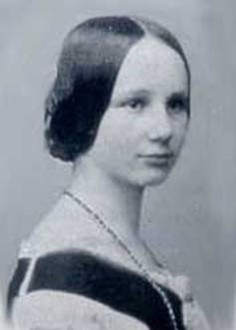
\includegraphics[width=0.6\columnwidth]{../img/ada}
\end{minipage}%
\begin{itemize}
\item \href{https://sv.wikipedia.org/wiki/Programmering}{sv.wikipedia.org/wiki/Programmering}
\item \href{https://en.wikipedia.org/wiki/Computer\_programming}{en.wikipedia.org/wiki/Computer\_programming}
\item Ha picknick i \href{http://kartor.lund.se/wiki/lundanamn/index.php/Ada_Lovelace-parken}{Ada Lovelace-parken} på Brunnshög!
\end{itemize}
\end{Slide}


\begin{Slide}{Vad är en kompilator?}
\begin{minipage}{.35\textwidth}
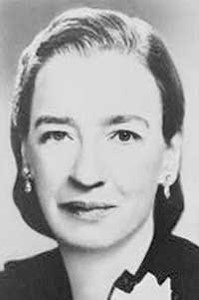
\includegraphics[width=0.6\textwidth]{../img/grace}
\end{minipage}%
\begin{minipage}{.67\textwidth}
%https://www.sharelatex.com/blog/2013/08/29/tikz-series-pt3.html
\begin{tikzpicture}[node distance=1.4cm,scale=0.8]
  \node (input) [startstop] {Källkod};
  \node(inptext) [right of=input, text width=2cm, scale=0.8,xshift=1.5cm]{För\\människor};
  \node (compile) [process, below of=input] {Kompilator};
  \node (output) [startstop, below of=compile] {Maskinkod};
  \node(outtext) [right of=output, text width=2cm, scale=0.8,xshift=1.5cm]{För\\maskiner};
  \draw [arrow] (input) -- (compile);
  \draw [arrow] (compile) -- (output);
  \end{tikzpicture}%

\vspace{1em}\noindent Grace Hopper uppfann kompilatorn 1952. \\ \href{https://en.wikipedia.org/wiki/Grace\_Hopper}{\SlideFontTiny en.wikipedia.org/wiki/Grace\_Hopper}
\end{minipage}%
\end{Slide}


\begin{Slide}{Virtuell maskin (VM) == abstrakt hårdvara}
\begin{multicols}{2}
\begin{itemize}
\item En VM är en ''dator'' implementerad i mjukvara som kan tolka en generell ''maskinkod'' som \Emph{översätts under körning} till den \Alert{verkliga} maskinens specifika maskinkod.

\item Med en VM blir källkoden \Emph{plattformsoberoende} och fungerar på många olika maskiner.

\item Exempel JVM: \\ \Emph{Java Virtual Machine}


\end{itemize}

\columnbreak %---------

%https://www.sharelatex.com/blog/2013/08/29/tikz-series-pt3.html
\begin{tikzpicture}[node distance=1.4cm]
\node (input) [startstop] {Källkod};
\node (compile) [process, below of=input] {Kompilator};
\node (output) [startstop, below of=compile] {Generell ''maskinkod''};
\node (interp) [process, below of=output] {VM interpreterar};
\node (output2) [startstop, below of=interp] {Specifik maskinkod};
\draw [arrow] (input) -- (compile);
\draw [arrow] (compile) -- (output);
\draw [arrow] (output) -- (interp);
\draw [arrow] (interp) -- (output2);
\end{tikzpicture}
\end{multicols}
\end{Slide}

\begin{Slide}{Vad består ett program av?}
\begin{itemize}
\item Text som följer entydiga språkregler (grammatik):
\begin{itemize}
\item \Emph{Syntax}: textens konkreta utseende
\item \Emph{Semantik}: textens betydelse (vad maskinen gör/beräknar)
\end{itemize}
\item \Emph{Nyckelord}: ord med speciell betydelse, t.ex. \code{if}, \code{else}
\item \Emph{Deklarationer}: definitioner av nya ord: \code{def gurka = 42}
\item \Emph{Satser} är instruktioner som \Alert{gör} något: \code{print("hej")}
\item \Emph{Uttryck} är instruktioner som beräknar ett \Alert{resultat}: \code{1 + 1}
\item \Emph{Data} är information som behandlas: t.ex. heltalet \code{42}
\item Instruktioner ordnas i kodstrukturer: \Alert{SARA}
\begin{itemize}
  \item \Emph{Sekvens}: ordningen spelar roll för vad som händer
  \item \Emph{Alternativ}: olika resultat beroende på uttrycks värde
  \item \Emph{Repetition}: instruktioner upprepas många gånger
  \item \Emph{Abstraktion}: nya byggblock skapas för att återanvändas
\end{itemize}
\end{itemize}
\end{Slide}

\begin{Slide}{Exempel på programmeringsspråk}
Det finns massor med olika språk och det kommer ständigt nya.
\vspace{1em}
\begin{multicols}{2}
Exempel:
\begin{itemize}
\item Java
\item C
\item C++
\item C\#
\item Python
\item JavaScript
\item Scala
\end{itemize}

\columnbreak %---------

Topplistor:
\begin{itemize}
\item \href{https://redmonk.com/sogrady/2020/07/27/language-rankings-6-20/}{Redmonk language rankings}   
%\item \href{https://redmonk.com/sogrady/2019/07/18/language-rankings-6-19/}{Redmonk language rankings}   
%\item \href{https://redmonk.com/sogrady/2018/08/10/language-rankings-6-18/}{Redmonk language rankings}   
\item \href{http://pypl.github.io/PYPL.html}{PYPL Index}
\item \href{http://www.tiobe.com/index.php/content/paperinfo/tpci/index.html}{TIOBE Index}
\end{itemize}
% \vspace{1em}
% 
\includegraphics[width=0.8\columnwidth]{../img/pypl}\\\SlideFontSmall{[PYPL (2016)]}
\end{multicols}

\end{Slide}

\ifkompendium\else
\begin{SlideExtra}{Redmonk Language Rankings: Github, Stackoverflow}
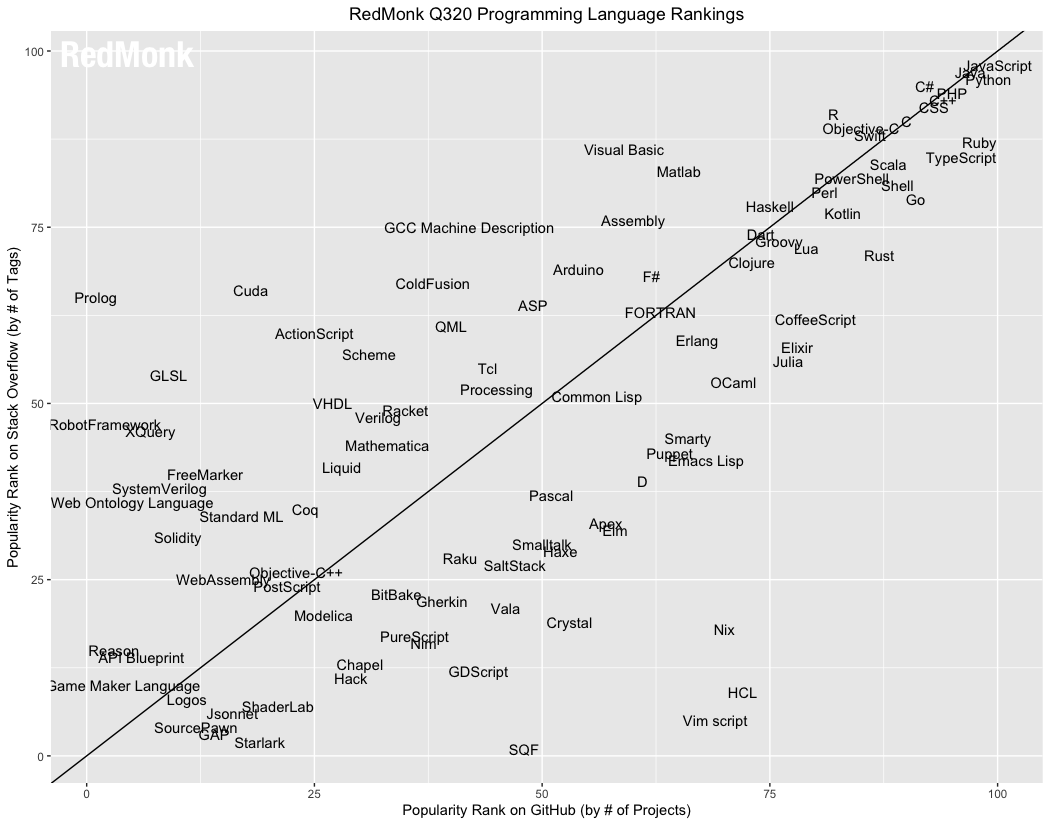
\includegraphics[width=0.95\columnwidth]{../img/redmonk-Q320}
\end{SlideExtra}
\begin{SlideExtra}{Några språks utveckling över tid enl. PYPL}
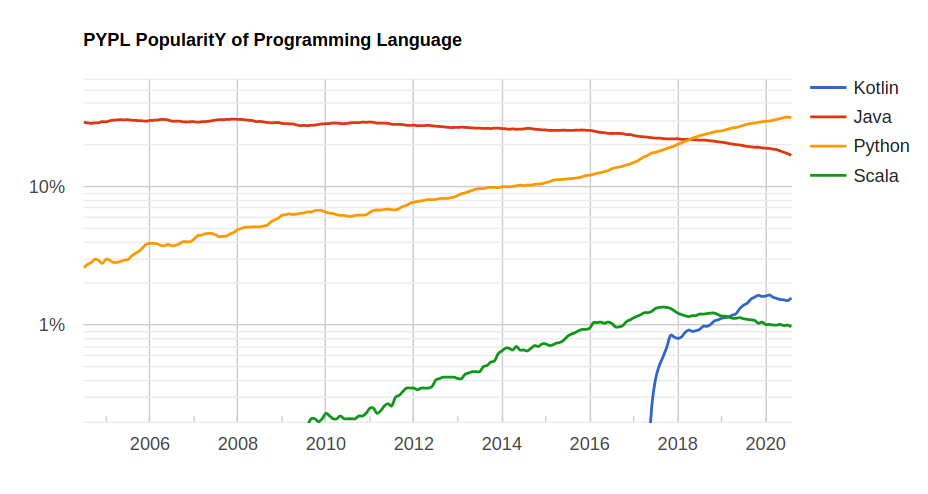
\includegraphics[width=0.95\columnwidth]{../img/pypl-06-20}
\end{SlideExtra}

\fi

\begin{Slide}{Olika programmeringsparadigm}
\begin{itemize}
\item Det finns många olika \href{https://en.wikipedia.org/wiki/Programming_paradigm}{programmeringsparadigm} (sätt att programmera på), till exempel:
\begin{itemize}\SlideFontSmall
\item \Emph{imperativ programmering:} programmet är uppbyggt av sekvenser av olika satser som påverkar systemets tillstånd
\item \Emph{objektorienterad programmering:} en sorts imperativ programmering där programmet består av objekt som sammanför data och operationer på dessa data
\item \Emph{funktionsprogrammering:} programmet är uppbyggt av samverkande (matematiska) funktioner som undviker föränderlig data och tillståndsändringar
\item \Emph{deklarativ programmering, logikprogrammering:} programmet är uppbyggt av logiska uttryck som beskriver olika fakta eller villkor och exekveringen utgörs av en bevisprocedur som söker efter värden som uppfyller fakta och villkor
\end{itemize}
\end{itemize}
\end{Slide}


\begin{Slide}{Hello world}

Scala-skript:
\begin{REPLnonum}
scala> println("Hello World!")
Hello World!
\end{REPLnonum}

Scala-applikation:
\begin{Code}
object Hello {
  def main(args: Array[String]): Unit = println("Hello world!")
}
\end{Code}

Java-applikation:
\begin{Code}[language=Java]
public class Hello {
    public static void main(String[] args) {
        System.out.println("Hello world!");
    }
}
\end{Code}

\end{Slide}

\begin{Slide}{Utvecklingscykeln}
editera; kompilera; hitta fel och förbättringar; editera; kompilera; hitta fel och förbättringar; editera; kompilera; hitta fel och förbättringar; editera; kompilera; hitta fel och förbättringar; editera; kompilera; hitta fel och förbättringar; editera; kompilera; hitta fel och förbättringar; ...

\begin{Code}
upprepa(1000){
  editera
  kompilera
  testa
}
\end{Code}
\end{Slide}

\begin{Slide}{Utvecklingsverktyg}
\begin{itemize}
\item Din verktygskunskap är mycket viktig för din produktivitet.
\item Lär dig kortkommandon för vanliga handgrep.
\item Verktyg vi använder i kursen:
\begin{itemize}
\item Scala \Emph{REPL}: från övn 1
\item \Emph{Texteditor} för kod, t.ex VS \code{code}: från övn 2
\item Kompilera med \Emph{\code{scalac}} och \Emph{\code{javac}}: från övn 2
\item Integrerad utvecklingsmiljö (IDE)
\begin{itemize}
\item \Emph{Kojo}: från lab 1
\item \Emph{IntelliJ IDEA} (alt. ScalaIDE/Eclipse): från läsperiod 2
\end{itemize}
\item \Emph{jar} för att packa ihop och distribuera klassfiler
\item \Emph{javadoc} och \Emph{scaladoc} för dokumentation av kodbibliotek
\end{itemize}
\item Andra verktyg som är bra att lära sig:
\begin{itemize}
\item git för versionshantering
\item GitHub för kodlagring -- men \Alert{inte} av lösningar till labbar!
\end{itemize}
\end{itemize}
\end{Slide}





\Subsection{De enklaste beståndsdelarna: litteraler, uttryck, variabler}


\begin{Slide}{Litteraler}
\begin{itemize}
\item En literal representerar ett fixt \Emph{värde} i koden och används för att skapa \Alert{data} som programmet ska bearbeta.
\item Exempel: \\
\begin{tabular}{l l}
\code|42| & heltalslitteral\\
\code|42.0| & decimaltalslitteral\\
\code|'!'| & teckenlitteral, omgärdas med 'enkelfnuttar' \\
\code|"hej"| & stränglitteral, omgärdas med ''dubbelfnuttar'' \\
\code|true| & litteral för sanningsvärdet ''sant''\\
\end{tabular}
\item Literaler har en \Emph{typ} som avgör vad man kan göra med dem.
\end{itemize}
\end{Slide}

\begin{Slide}{Exempel på inbyggda datatyper i Scala}\SlideFontSmall
\begin{itemize}
\item Alla värden, uttryck och variabler har en \href{https://sv.wikipedia.org/wiki/Datatyp}{\Emph{datatyp}}, t.ex.:
\begin{itemize}\footnotesize
\item \code{Int} för heltal
\item \code{Long} för \textit{extra} stora heltal (tar mer minne)
\item \code{Double} för decimaltal, så kallade flyttal med flytande decimalpunkt
\item \code{String} för strängar
\end{itemize}

\item Kompilatorn håller reda på att uttryck kombineras på ett \Emph{typsäkert} sätt. Annars blir det \Alert{kompileringsfel}.

\item Scala och Java är s.k. \href{https://sv.wikipedia.org/wiki/Typsystem}{\Emph{statiskt typade}} språk, vilket innebär att kontroll av typinformation sker vid kompilering \Eng{compile time}\footnote{Andra språk, t.ex. Python och Javascript är \Emph{dynamiskt typade} och där skjuts typkontrollen upp till körningsdags \Eng{run time} \\ Vilka är för- och nackdelarna med statisk vs. dynamisk typning?}.

\item Scala-kompilatorn gör \href{https://en.wikipedia.org/wiki/Type_inference}{\Emph{typhärledning}}: man \Alert{slipper skriva typerna} om kompilatorn kan lista ut dem med hjälp av typerna hos deluttrycken.

\end{itemize}
\end{Slide}


\begin{Slide}{Grundtyper i Scala}\SlideFontSmall
Dessa \Emph{grundtyper} \Eng{basic types} finns inbyggda i Scala:

\begin{table}[H]
\renewcommand{\arraystretch}{1.4}
\begin{tabular}{p{0.24\textwidth}|p{0.21\textwidth}|l}
\textit{Svenskt namn} & \textit{Engelskt namn} & \Emph{Grundtyper} \\ \hline
heltalstyp & integral type & \texttt{Byte}, \texttt{Short}, \texttt{Int}, \texttt{Long}, \texttt{Char} \\
flyttalstyp  &  floating point \newline number types & \texttt{Float}, \texttt{Double} \\
numeriska typer & numeric types & heltalstyper och flyttalstyper \\
strängtyp \newline (teckensekvens) & string type & \texttt{String}  \\
sanningsvärdestyp  \newline (boolesk typ)& truth value type & \texttt{Boolean} \\
\end{tabular}
\end{table}

\end{Slide}

\begin{Slide}{Grundtypernas implementation i JVM}\SlideFontSmall
\begin{table}[H]
\renewcommand{\arraystretch}{1.4}
\begin{tabular}{l|l|l|l}
\Alert{Grundtyp} i &  Antal                &      Omfång&\Alert{primitiv typ} i\\
 \Emph{Scala} & bitar & minsta/största värde &\Emph{Java} \& \Emph{JVM}\\ \hline
\texttt{Byte}   &  8  & $-2^7$ ... $2^7-1$   & \texttt{byte} \\
\texttt{Short}  &  16 & $-2^{15}$ ... $2^{15}-1$ & \texttt{short} \\
\texttt{Char}   &  16 & $0$ ... $2^{16}-1$ & \texttt{char} \\
\texttt{Int}    &  32 & $-2^{31}$ ... $2^{31}-1$ & \texttt{int} \\
\texttt{Long}   &  64 & $-2^{63}$ ... $2^{63}-1$ & \texttt{long} \\
\texttt{Float}  &  32 & ± $3.4028235 \cdot 10^{38}$  & \texttt{float} \\
\texttt{Double} &  64 & ± $1.7976931348623157 \cdot 10^{308}$ & \texttt{double} \\
\end{tabular}
\end{table}

Grundtypen \texttt{String} lagras som en \emph{sekvens} av 16-bitars tecken av typen \texttt{Char} och kan vara av godtycklig längd (tills minnet tar slut).

\end{Slide}


\begin{Slide}{Uttryck}
\begin{itemize}
\item Ett \Emph{uttryck} består av en eller flera delar som efter \Emph{evaluering} ger ett \Alert{resultat}.
\item Delar i ett uttryck kan t.ex. vara: \\ literaler (42), operatorer (+), funktioner (sin), ...
\item Exempel:
\begin{itemize}
\item Ett enkelt uttryck: \\ \code{42.0}
\item Sammansatta uttryck: \\
\code{40 + 2} \\
\code{(20 + 1) * 2} \\
\code{sin(0.5 * Pi)} \\
\code{"hej" + " på " + "dej"}
\end{itemize}

\item När programmet tolkas sker \Emph{evaluering} av uttrycket, vilket ger ett resultat i form av ett \Emph{värde} som har en \Emph{typ}.
\end{itemize}
\end{Slide}


\begin{Slide}{Variabler}\SlideFontSmall
\begin{itemize}
\item En \Emph{variabel} kan tilldelas värdet av ett enkelt eller sammansatt uttryck.
\item En variabel har ett \Emph{variabelnamn}, vars utformning följer språkets regler för s.k. \Emph{identifierare}.
\item En ny variabel införs i en \Emph{variabeldeklaration} och då den kan ges ett värde, \Emph{initialiseras}. Namnet användas som \Emph{referens} till värdet.
\item Exempel på variabeldeklarationer i Scala, notera \Emph{nyckelordet} \code{val}:
\begin{Code}
val a = 0.5 * Pi
val length = 42 * sin(a)
val exclamationMarks = "!!!"
val greetingSwedish = "Hej på dej" + exclamationMarks
\end{Code}

\item Vid exekveringen av programmet lagras variablernas värden i minnet och deras respektive värde hämtas ur minnet när de \Emph{refereras}.

\item Variabler som deklareras med \code{val} kan endast tilldelas ett värde \Alert{en enda gång}, vid den initialisering som sker vid deklarationen.
\end{itemize}

\end{Slide}


\begin{Slide}{Regler för identifierare}
\begin{itemize}
\item \Emph{Enkel} identifierare: t.ex. \code{gurka2tomat}
\begin{itemize}
\item Börja med bokstav
\item ...följt av bokstäver eller siffror
\item Kan även innehålla understreck
\end{itemize}

\item \Emph{Operator}-identifierare, t.ex. \code{+:}
\begin{itemize}
\item Börjar med ett \Emph{operatortecken}, t.ex. \code{+ - * / : ? ~ #}
\item Kan följas av fler operatortecken
\end{itemize}


\item En identifierare får \Alert{inte} vara ett \Emph{reserverat ord}, se \href{http://cs.lth.se/pgk/quickref}{snabbreferensen} för alla reserverade ord i Scala \& Java.

\item \Emph{Bokstavlig} identifierare: \code{`kan innehålla allt`}
\begin{itemize}
\item Börjar och slutar med \Emph{backticks}  \code{` `}
\item Kan innehålla vad som helst (utom backticks)
\item Kan användas för att undvika krockar med reserverade ord: \texttt{\code{`}val\code{`}}
\end{itemize}

\end{itemize}
\end{Slide}



%\begin{Slide}{Regler för identifierare i Java}\footnotesize
%När kompilatorn ''läser''  \footnote{man säger ofta ''parsa'' i stället för ''läsa'' när kompilatorn tolkar koden} koden och och försöker hitta variabelnamn, antar den att du följer de entydiga syntaktiska reglerna för språket.  \\ \vskip1em För namn i Java gäller följande regler: %https://docs.oracle.com/javase/tutorial/java/nutsandbolts/variables.html
%\begin{itemize}
%\item Namn får inte vara \href{https://docs.oracle.com/javase/tutorial/java/nutsandbolts/_keywords.html}{reserverade ord}
%\item Stora och små bokstäver spelar roll \Eng{case sensistive} \\ \lstinline{int highScore;} och \lstinline{int highscore;} ger alltså två \textit{olika} variabler
%\item Namnet måste börja med en bokstav, ett understreck \_ eller ett dollartecken \$
%\item Namn får \textit{inte} innehålla blanktecken
%\item Namn får innehålla bokstäver, siffror, understreck \_ och dollartecken \$, men \textit{inte} andra specialtecken (alltså inte \lstinline~%&@!{(})/+-*~ etc.)
%\end{itemize}
%\end{Slide}



\begin{Slide}{Att bygga strängar: konkatenering och interpolering}
\begin{itemize}
\item Man kan \Emph{konkatenera} strängar med operatorn + \\ \code{"hej" + " på " + "dej"}
\item Efter en sträng kan man konkatenera vilka uttryck som helst; uttryck inom parentes evalueras först och värdet görs sen om till en sträng före konkateneringen:
\begin{Code}
val x = 42
val msg = "Dubbla värdet av " + x + " är " + (x * 2) + "."
\end{Code}
\item Man kan i Scala (men inte Java) få hjälp av kompilatorn att övervaka bygget av strängar med \Emph{stränginterpolatorn} \Alert{s}:
\begin{Code}
val msg = s"Dubbla värdet av $x är ${x * 2}."
\end{Code}

\end{itemize}
\end{Slide}

\begin{Slide}{Heltalsaritmetik}\SlideFontSmall
\begin{itemize}
\item De fyra räknesätten skrivs som i matematiken (vanlig \href{https://en.wikipedia.org/wiki/Order_of_operations}{precedens}):
\begin{REPL}
scala> 3 + 5 * 2 - 1
res0: Int = 12
\end{REPL}
\item \Emph{Parenteser} styr \Alert{evalueringsordningen}:
\begin{REPL}
scala> (3 + 5) * (2 - 1)
res1: Int = 8
\end{REPL}
\item \Emph{Heltalsdivision} sker med \Alert{decimaler avkortade}:
\begin{REPL}
scala> 41 / 2
res2: Int = 20
\end{REPL}
\item \href{https://en.wikipedia.org/wiki/Modulo_operation}{\Emph{Moduloräkning}} med restoperatorn \code{%}
\begin{REPL}
scala> 41 % 2
res3: Int = 1
\end{REPL}
\end{itemize}
\end{Slide}


\begin{Slide}{Flyttalsaritmetik}\SlideFontSmall
\begin{itemize}
\item Decimaltal representeras med s.k. \href{https://sv.wikipedia.org/wiki/Flyttal}{\Emph{flyttal}} av typen \code{Double}:
\begin{REPL}
scala> math.Pi
res4: Double = 3.141592653589793
\end{REPL}

\item Stora tal så som $\pi*10^{12}$ skrivs:
\begin{REPL}
scala> math.Pi * 1E12
res5: Double = 3.141592653589793E12
\end{REPL}
\item Det finns \Alert{inte} oändligt antal decimaler vilket ger problem med \Alert{avvrundingsfel}:
\begin{REPL}
scala> 0.0000000000001
res6: Double = 1.0E-13

scala> 1E10 + 0.0000000000001
res7: Double = 1.0E10
\end{REPL}
\end{itemize}
\end{Slide}

% \ifkompendium\else
% \begin{SlideExtra}{På rasten}
% En per grupp kommer fram hit och tar en grupp-skylt
% \begin{itemize}
%   \item Samlas i era samarbetsgrupper i foajen
%   \item D1.01a längst västerut (mot havet), D1.12b längst österut
%   \item Lär allas namn
%   \item Bestäm tid för första möte
%   \item Vid behov: \\ Bestäm vem som mejlar till de i gruppen som inte är här idag 
% \end{itemize}  
% \end{SlideExtra}
% \fi

\Subsection{Funktioner}

\begin{Slide}{Definiera namn på uttryck}
\begin{itemize}
\item Med nyckelordet \code{def} kan man låta ett \Emph{namn} betyda samma sak som ett \Emph{uttryck}.
\item Exempel:
\begin{Code}
def gurklängd = 42 + x
\end{Code}
\item Uttrycket till höger evalueras \Alert{varje} gång \Emph{anrop} sker,\\
d.v.s. varje gång namnet används på annat ställe i koden.
\begin{Code}
gurklängd
\end{Code}

\end{itemize}
\end{Slide}

\begin{Slide}{Funktion, argument, parameter}\SlideFontSmall
\begin{itemize}
\item En \Emph{funktion} räknar ut \Alert{resultat} baserat på indata som kallas \Emph{argument}.

\item Argument ges namn genom deklaration av \Emph{parametrar}.

\item Exempel på deklaration av en funktion med en parameter:
\begin{Code}
def dubblera(x: Int) = 2 * x
\end{Code}

\item Parametrarnas typ \Alert{måste} beskrivas efter \Emph{kolon}.
\item Kompilatorn kan härleda \Emph{returtypen}, men den kan också med fördel, för tydlighetens skull, anges \Alert{explicit}:
\begin{Code}
def dubblera(x: Int): Int = 2 * x
\end{Code}

\item Observera att namnet \code{x} blir ett ''nytt fräscht'' \Emph{lokalt namn} som \Alert{bara finns och syns  ''inuti'' funktionen} och har inget med ev. andra \code{x} utanför funktionen att göra.

\item Beräkningen sker först vid \Alert{anrop} av funktionen:
\begin{REPL}
scala> dubblera(42)
res1: Int = 84
\end{REPL}

\end{itemize}
\end{Slide}






\begin{Slide}{Färdiga matte-funktioner i paketet \texttt{scala.math}}\SlideFontSmall
\begin{itemize}
\item I paketet \texttt{\Emph{scala.math}} finns många användbara funktioner: t.ex.\\
\code{math.random()} ger slumptal mellan \code{0.0} och \code{0.99999999999999999}
\begin{REPLnonum}
scala> val x = math.random()
x: Double = 0.27749191749889635

scala> val length = 42.0 * math.sin(math.Pi / 3.0)
length: Double = 36.373066958946424
\end{REPLnonum}

\item Studera dokumentationen här: \\{\SlideFontTiny
\url{http://www.scala-lang.org/api/current/scala/math/}}

\item Paketet \code{scala.math} delegerar ofta till Java-klassen \texttt{\Emph{java.lang.Math}} som är dokumenterad här: \\{\SlideFontTiny
\url{https://docs.oracle.com/javase/8/docs/api/java/lang/Math.html}}

\end{itemize}
\end{Slide}



\Subsection{Logik}

\begin{Slide}{Logiska uttryck}\SlideFontSmall
\begin{minipage}{.8\textwidth}
\begin{itemize}
\item Datorn kan ''räkna'' med sanning och falskhet: \\
s.k. \href{https://en.wikipedia.org/wiki/Boolean_algebra}{booelsk algebra} efter \href{https://en.wikipedia.org/wiki/George_Boole}{George Boole}

\item Enkla logiska uttryck: (finns bara två stycken)
\begin{itemize}
\item[] \code{true}
\item[] \code{false}
\end{itemize}
\end{itemize}
\end{minipage}%
\begin{minipage}{.2\textwidth}
\centering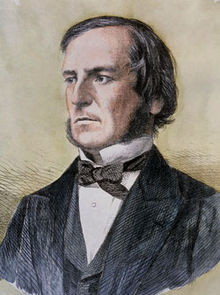
\includegraphics[width=0.9\columnwidth]{../img/boole}
\end{minipage}%
\begin{itemize}


\item Sammansatta logiska uttryck med logiska operatorer:\\
\code{&&} och, \texttt{||} eller, \texttt{!} icke, \code{==} likhet, \code{!=} olikhet,
relationer: \code{> < >= <=}

\item Exempel:
\begin{itemize}
\item[] \code{true && true}
\item[] \code{false || true}
\item[] \code{!false}
\item[] \code{42 == 43}
\item[] \code{42 != 43}
\item[] \code{(42 >= 43) || (1 + 1 == 2)}
\end{itemize}

\end{itemize}
\end{Slide}

\begin{Slide}{De Morgans lagar}

\href{https://en.wikipedia.org/wiki/Augustus_De_Morgan}{\Emph{De Morgans lagar}} beskriver vad som händer om man \Alert{negerar} ett logiskt uttryck. Kan användas för att göra \Emph{förenklingar}.

%$p$ och $q$ är logiska uttryck, $\neg$ står för ''icke'', $\wedge$ för ''och'', $\vee$ för ''eller'':
%\begin{eqnarray*}
%\neg (p \wedge q) & \Longleftrightarrow & (\neg p) \vee (\neg q)\\
%\neg (p \vee q) & \Longleftrightarrow & (\neg p) \wedge (\neg q)\\
%\end{eqnarray*}

\begin{itemize}
\item I all deluttryck sammanbundna med \code{&&} eller \code{||}, \\ ändra alla \code{&&} till \code{||} och omvänt.
\item Negera alla ingående deluttryck. En relation negeras genom att man byter \texttt{==} mot \texttt{!=}, \texttt{<} mot \texttt{>=}, etc.
\end{itemize}

Exempel på förenkling där de Morgans lagar används upprepat:

\begin{Code}[escapechar=X,backgroundcolor=,frame=none,basicstyle=\ttfamily\fontsize{10}{12}\selectfont]
! (a < b || (a == 1 && b == 1))             X$\iff$X
! (a < b) && ! (a == 1 && b == 1)           X$\iff$X
! (a < b) && (! (a == 1) || ! (b == 1))     X$\iff$X
a >= b && (a != 1 || b != 1)
\end{Code}
\end{Slide}

\begin{Slide}{Alternativ med if-uttryck}
\begin{itemize}
\item Ett if-uttryck börjar med nyckelordet \code{if}, följt av ett logiskt uttryck inom parentes och två grenar.
\begin{Code}
def slumpgrönsak = if (math.random() < 0.8) "gurka" else "tomat"
\end{Code}
\item Den ena grenen evalueras om uttrycket är \code{true}
\item Den andra \code{else}-grenen evalueras om uttrycket är \code{false}
\begin{REPLnonum}
scala> slumpgrönsak
res13: String = gurka

scala> slumpgrönsak
res14: String = gurka

scala> slumpgrönsak
res15: String = tomat

\end{REPLnonum}
\end{itemize}
\end{Slide}

\Subsection{Satser}


%%%%%%%%%%%%%%%%%%%%%%%%
\begin{Slide}{Variabeldeklaration och tilldelningssats}\SlideFontTiny

\begin{itemize}
\item En \Emph{variabeldeklaration} medför att \Alert{plats i datorns minne} reserveras så att värden av den typ som variabeln kan referera till får plats där.

\item Vid deklaration ska variabeln \Emph{initialiseras} med ett startvärde.

\item En \code{val}-deklaration ger en variabel som efter initialisering inte kan ändras.


\begin{multicols}{2}
Dessa deklarationer...
\begin{lstlisting}
var x = 42
val y = x + 1
\end{lstlisting}
... ger detta innehåll någonstans i minnet:

%http://tex.stackexchange.com/questions/18521/tikz-matrix-as-a-replacement-for-tabular
\begin{tikzpicture}[]
\matrix [matrix of nodes, row sep=0, column 2/.style={nodes={rectangle,draw,minimum width=3em}}]
{
x   & 42 \\
y   & 43 \\
};
\end{tikzpicture}
%\end{column}

%\end{columns}

\end{multicols}


\item Med en \Emph{tilldelningssats} ges en tidigare \code{var}-deklarerad variabel ett nytt värde:
\begin{lstlisting}
x = 13
\end{lstlisting}

\item Det gamla värdet försvinner för alltid och det nya värdet lagras istället: \\
\begin{tikzpicture}[]
\matrix [matrix of nodes, row sep=0, column 2/.style={nodes={rectangle,draw,minimum width=3em}}]
{
x   & 13 \\
y   & 43 \\
};
\end{tikzpicture}

Observera att \code{y} här inte påverkas av att x ändrade värde.
\end{itemize}
\end{Slide}

\begin{Slide}{Tilldelningssatser är \emph{inte} matematisk likhet}\SlideFontSmall

\begin{itemize}

\item Likhetstecknet används alltså för att \Emph{tilldela} variabler nya värden och det är \Alert{inte} samma sak som matematisk likhet. Vad händer här?
\begin{lstlisting}
x = x + 1
\end{lstlisting}

\item Denna syntax är ett arv från de gamla språken C, Fortran mfl.

\item I \href{https://en.wikipedia.org/wiki/Assignment_(computer_science)}{andra språk} används  t.ex.  \\\vspace{1em}
\texttt{x := x + 1}  \hspace{2em} eller  \hspace{2em} \texttt{x <- x + 1} \\\vspace{0.5em}

\item Denna syntax visar kanske bättre att tilldelning är en \Emph{stegvis process}:

\begin{enumerate}\SlideFontTiny
\item Först beräknas \Emph{uttrycket till höger} om tilldelningstecknet.
\item Sedan \Emph{ersätts värdet} som variabelnamnet refererar till av det beräknade uttrycket. Det gamla värdet \Alert{försvinner för alltid}.
\end{enumerate}

\end{itemize}

\end{Slide}


\begin{Slide}{Förkortade tilldelningssatser}
\begin{itemize}
\item Det är vanligt att man vill tilldela en variabel ett nytt värde som beror av det gamla, så som i \\\code{x = x + 1}

\item Därför finns \Emph{förkortade tilldelningssatser} som gör så att man sparar några tecken och det blir tydligare (?) vad som sker (när man vant sig vid detta skrivsätt):
\begin{Code}
x += 1
\end{Code}

\item Uttrycket ovan expanderas av kompilatorn till \code{x = x + 1}
\end{itemize}


\end{Slide}


\begin{Slide}{Exempel på förkortade tilldelningssatser}
\begin{REPLnonum}
scala> var x = 42
x: Int = 42

scala> x *= 2

scala> x
res0: Int = 84


scala> x /= 3

scala> x
res2: Int = 28
\end{REPLnonum}
\end{Slide}


\ifkompendium\else
\begin{Slide}{Övning: Tilldelningar i sekvens}\footnotesize

%\begin{columns}
%\begin{column}{0.32\textwidth}
\begin{minipage}{0.32\textwidth}

Rita hur minnet ser ut efter varje rad nedan:
\vskip1em
\begin{lstlisting}[ numbers=left,]
var u = 42
var x = 10
var y = 2 * x + 1
x = 20
var z = y + x + y - x
x += 1; y *= 2
\end{lstlisting}
%\end{column}
\end{minipage}\hspace{2em}%
%\begin{column}{0.6\textwidth}
\begin{minipage}{0.6\textwidth}


\scriptsize En variabel som ännu inte \Emph{initierats} har ett \Alert{odefinierat} värde, anges nedan med frågetecken.
\begin{table}[]
\centering\scriptsize
%http://tex.stackexchange.com/questions/83930/what-are-the-different-kinds-of-boxes-in-latex
\newcommand{\mybox}[1]{\raisebox{-0.5mm}{\framebox(21,14){#1}}\vspace{0.5mm}}
\begin{tabular}{@{}ccccccc}
 & rad 1 & rad 2 & rad 3 & rad 4  & rad 5 & rad 6\\
u& \mybox{42 } &  \mybox{}   &   \mybox{}   & \mybox{} & \mybox{} & \mybox{} \\
x& \mybox{? } &  \mybox{}   &   \mybox{}   & \mybox{} & \mybox{}  & \mybox{} \\
y& \mybox{? } &  \mybox{}   &   \mybox{}   & \mybox{} & \mybox{}  & \mybox{} \\
z& \mybox{? } &  \mybox{}   &   \mybox{}   & \mybox{} & \mybox{}  & \mybox{} \\
\end{tabular}
\end{table}

%\end{column}
%\end{columns}
\end{minipage}%
\end{Slide}
\fi



\begin{Slide}{Variabler som ändrar värden kan vara knepiga}
\begin{itemize}
\item Kod som innehåller variabler som \Alert{förändras} över tid är ofta svårare att läsa och begripa.

\item Många buggar beror på att variabler av misstag förändras på felaktiga och oanade sätt.

\item Föränderliga värden blir speciellt svåra i kod som körs jämlöpande (parallellt).

\item I kod som körs i skarpt läge med många användare (s.k. produktionskod) är därför \code{val} att föredra, medan \code{var} endast används om det \Alert{verkligen} behövs.
\item Alltså: räkna hellre ut nya värden än förändra befintliga.
\end{itemize}
\end{Slide}
%%%%%%%%%%



\begin{Slide}{Kontrollstrukturer: alternativ och repetition}\SlideFontSmall
Används för att kontrollera (förändra) sekvensen och skapa \Emph{alternativa} vägar genom koden. Vägen  bestäms vid körtid.
\begin{itemize}
\item if-sats:
\begin{Code}
if (math.random() < 0.8) println("gurka") else println("tomat")
\end{Code}
\end{itemize}

Olika sorters \Emph{loopar} för att repetera satser. Antalet repetitioner ges vid körtid.
\begin{itemize}
\item \code{while}-sats: bra när man \Alert{inte vet hur många gånger} det kan bli.
\begin{Code}
while (math.random() < 0.8) println("gurka")
\end{Code}

\item \code{for}-sats: bra när man \Alert{vill ange antalet repetitioner}:
\begin{Code}
for (i <- 1 to 10) println(s"gurka nr $i")
\end{Code}

\end{itemize}
\end{Slide}

%%%% GE mer detaljer eller överlåta till övning???
%\begin{Slide}{if-sats}
%\begin{itemize}
%\item
%\end{itemize}
%\end{Slide}
%
%\begin{Slide}{while-sats}
%\begin{itemize}
%\item
%\end{itemize}
%\end{Slide}
%
%\begin{Slide}{for-sats}
%\begin{itemize}
%\item
%\end{itemize}
%\end{Slide}

\begin{Slide}{Procedurer}\SlideFontSmall
\begin{itemize}
\item En \Emph{procedur} är en funktion som \Alert{gör} något intressant, men som \Alert{inte} lämnar något intressant returvärde.
\item Exempel på procedur i standardbiblioteket: \code{println("hej")}
\item Du \Emph{deklarerar egna procedurer} genom att ange \texttt{\Alert{Unit}} som returvärdestyp. Då returneras värdet \texttt{\Alert{()}} som betyder ''inget''.
\end{itemize}
\begin{REPLnonum}
scala> def hej(x: String): Unit = println(s"Hej på dej $x!")
hej: (x: String)Unit

scala> hej("Herr Gurka")
Hej på dej Herr Gurka!

scala> val x = hej("Fru Tomat")
Hej på dej Fru Tomat!
x: Unit = ()
\end{REPLnonum}
\begin{itemize}
\item Det som \Alert{görs} kallas (sido)\Emph{effekt}. Ovan är utskriften själva effekten.
\item Även funktioner kan ha sidoeffekter. De kallas då \Alert{oäkta} funktioner.
\end{itemize}
\end{Slide}

\begin{Slide}{Problemlösning: nedbrytning i abstraktioner som sen kombineras}\SlideFontSmall
\begin{itemize}
\item En av de allra viktigaste principerna inom programmering är \Emph{funktionell nedbrytning} där  \Emph{underprogram} i form av funktioner och procedurer skapas för att bli byggstenar som kombineras till mer avancerade funktioner och procedurer.

\item Genom de namn som definieras skapas \Emph{återanvändbara abstraktioner} som kapslar in det funktionen gör till ett ''byggblock''.

\item Bra ''byggblock'' gör det lättare att lösa svåra programmeringsproblem.

\item Abstraktioner som beräknar eller gör \Emph{en enda, väldefinierad sak} är enklare att använda, jämfört med de som gör många, helt olika saker.

\item Abstraktioner med \Emph{välgenomtänkta namn} är enklare att använda, jämfört med kryptiska eller missvisande namn.
\end{itemize}

\end{Slide}

\ifkompendium\else

\begin{SlideExtra}{Om veckans övning: \code{expressions}}\SlideFontSmall

\begin{itemize}
%!TEX encoding = UTF-8 Unicode

\item Förstå vad som händer när satser exekveras och uttryck evalueras.
\item Förstå sekvens, alternativ och repetition.
\item Känna till literalerna för enkla värden, deras typer och omfång.
\item Kunna deklarera och använda variabler och tilldelning, samt kunna rita bilder av minnessituationen då variablers värden förändras.
\item Förstå skillnaden mellan olika numeriska typer, kunna omvandla mellan dessa och vara medveten om noggrannhetsproblem som kan uppstå.
\item Förstå booleska uttryck och värdena \code{true} och \code{false}, samt kunna förenkla booleska uttryck.
\item Förstå skillnaden mellan heltalsdivision och flyttalsdivision, samt användning av rest vid heltalsdivision.
\item Förstå precedensregler och användning av parenteser i uttryck.
\item Kunna använda \code{if}-satser och \code{if}-uttryck.
\item Kunna använda \code{for}-satser och \code{while}-satser.
\item Kunna använda \code{math.random()} för att generera slumptal i olika intervaller.
\item Kunna beskriva skillnader och likheter mellan en procedur och en funktion.

\end{itemize}

\end{SlideExtra}

\begin{SlideExtra}{Om veckans labb: \code{kojo}}
\begin{itemize}
%!TEX encoding = UTF-8 Unicode

\item Kunna kombinera principerna sekvens, alternativ, repetition, och abstraktion i skapandet av egna program om minst 20 rader kod.
\item Kunna förklara vad ett program gör i termer av sekvens, alternativ, repetition, och abstraktion.
\item Kunna tillämpa principerna sekvens, alternativ, repetition, och abstraktion i enkla algoritmer.
\item Kunna formatera egna program så att de blir lätta att läsa och förstå.
\item Kunna förklara vad en variabel är och kunna skriva deklarationer och göra tilldelningar.
\item Kunna genomföra upprepade varv i cykeln \emph{editera-exekvera-felsöka/förbättra} för att successivt bygga upp allt mer utvecklade program.

\end{itemize}
\end{SlideExtra}

\fi

%%%%%%%%%%%%%%%%%%%%%%%%%%%%%%%%%%%%%% nedan redan meddelat i introveckan
%\ifkompendium\else
%\Subsection{Meddelande från \href{http://lth.se/code}{Code@LTH}}
%\fi









%!TEX encoding = UTF-8 Unicode
%!TEX root = ../compendium1.tex

\renewcommand{\vecka}{2}

\chapter{Kodstrukturer}\label{chapter:W02}
\begin{itemize}[nosep]
\item samling: Range
\item for-uttryck
\item map
\item foreach
\item flatMap
\item algoritm vs implementation
\item pseudokod
\item algoritm: swap
\item algoritm: summering
\item algoritm: min/max
\item paket
\item import
\item filstruktur
\item jar
\item dokumentation
\item programlayout
\item JDK
\item konstanter vs föränderlighet
\item objektorientering
\item klasser
\item objekt
\item punktnotation
\item referensvariabler
\item referenstilldelning
\item anropa metoder
\item block
\item namnsynlighet
\item namnöverskuggning
\item SimpleWindow
\end{itemize}

%!TEX encoding = UTF-8 Unicode
%!TEX root = ../lect-week02.tex

%\Subsection{Samlingar och loopar}
\Subsection{Datastrukturer och kontrollstrukturer}


\begin{Slide}{Vad är en datastruktur?}\SlideFontSmall
\begin{itemize}
\item En \href{https://sv.wikipedia.org/wiki/Datastruktur}{datastruktur} är en struktur för organisering av data som...
\begin{itemize}\SlideFontTiny
\item kan innehålla \Alert{många} element,
\item kan refereras till med \Alert{ett} enda namn, och
\item ger möjlighet att komma åt de enskilda elementen.
\end{itemize}

\item En \Emph{samling} \Eng{collection} är en datastruktur som kan innehålla många element av \Alert{samma typ}.

\item Exempel på olika samlingar där elementen är organiserade på olika vis: \\ 
\vspace{0.5em}
\begin{tabular}{l c}
\Emph{Lista} & 
\includegraphics[width=5cm]{../img/list.pdf} \\
\Emph{Träd}  & 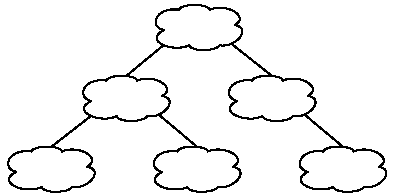
\includegraphics[width=2.2cm]{../img/tree.pdf} \\
\Emph{Graf}  & 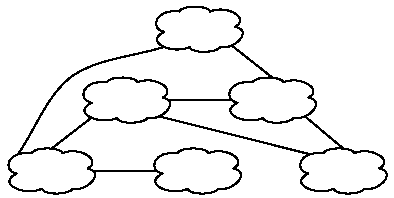
\includegraphics[width=2.2cm]{../img/graph.pdf} \\
\end{tabular}
\end{itemize}
{
\SlideFontTiny \vspace{1em }\hskip2em
Mer om listor \& träd \href{http://cs.lth.se/edaa01vt}{fördjupningskursen}. 
Mer om träd, grafer i \href{http://cs.lth.se/edaa40}{Diskreta strukturer.}
}

\end{Slide} 


\begin{Slide}{Vad är en vektor?}\SlideFontSmall
En \Emph{vektor}\footnote{Vektor kallas ibland på svenska även \href{https://sv.wikipedia.org/wiki/F\%C3\%A4lt_\%28datastruktur\%29}{fält}, men det skapar stor förvirring eftersom det engelska ordet \emph{field} ofta används för \emph{attribut} (förklaras senare).} 
\Eng{vector, \href{https://en.wikipedia.org/wiki/Array_data_structure}{array}} är en \Emph{samling} som är \Alert{snabb} att \Emph{indexera} i. 
Åtkomst av element sker med \code{apply(platsnummer)}: 

\begin{REPL}
scala> val heltal = Vector(42, 13, -1, 0 , 1)
heltal: scala.collection.immutable.Vector[Int] = Vector(42, 13, -1, 0, 1)

scala> heltal.apply(0)
res0: Int = 42

scala> heltal(1)    // man kan skippa .apply
res1: Int = 13

scala> heltal(5)
java.lang.IndexOutOfBoundsException: 5
  at scala.collection.immutable.Vector.checkRangeConvert(Vector.scala:132)
\end{REPL}
Utelämnar du \code{.apply} så gör kompilatorn anrop av \code{apply} ändå om det går.
\end{Slide}

\begin{Slide}{En konceptuell bild av en vektor}

\begin{REPLnonum}
scala> val heltal = Vector(42, 13, -1, 0 , 1)

scala> heltal(0)
res0: Int = 42
\end{REPLnonum}

\begin{tikzpicture}[font=\ttfamily]
\matrix [matrix of nodes, row sep=0, column 2/.style={nodes={rectangle,draw,minimum width=3em}}] (var) at (0cm, 2.8cm)
{
heltal   &  \makebox(16,12){ }\\
};
\matrix [matrix of nodes, draw=black,row sep=0, column 2/.style={nodes={rectangle,draw,minimum width=4em}}] (vec) at (4cm, 1cm)
{
\textit{plats} &  \\
0   &  \makebox(16,12){42}\\
1   &  \makebox(16,12){13}\\
2   &  \makebox(16,12){-1}\\
3   &  \makebox(16,12){0}\\
4   &  \makebox(16,12){1}\\
};
\filldraw[black] (0.7cm,2.8cm) circle (3pt) node[] (ref) {};
 \draw [arrow] (ref) -- (vec);
\end{tikzpicture}

%\vspace{1em} Elementen ligger på rad någonstans i minnet.
\end{Slide}



\begin{Slide}{En samling strängar}

\begin{itemize}
\item En vektor kan lagra många värden av samma typ. 
\item Elementen kan vara till exempel heltal eller strängar. 
\item Eller faktiskt vad som helst. 
\end{itemize}

\begin{REPL}
scala> val grönsaker = Vector("gurka","tomat","paprika","selleri")
grönsaker: scala.collection.immutable.Vector[String] = Vector(gurka, tomat, paprika, selleri)

scala> val g = grönsaker(1)
g: String = tomat

scala> val xs = Vector(42, "gurka", true, 42.0)
xs: scala.collection.immutable.Vector[Any] = Vector(42, gurka, true, 42.0)


\end{REPL}

\end{Slide}

\begin{Slide}{Vad är en kontrollstruktur?}
\begin{itemize}
\item En \Emph{kontrollstruktur} påverkar \Alert{sekvensen}.
\begin{itemize}
\item[] Exempel på inbyggda kontrollstrukturer: 
\\\vspace{0.5em}\code{for}-sats, \code{while}-sats
\end{itemize}

\item[]

\item I Scala kan man definiera \Emph{egna} kontrollstrukturer.
\begin{itemize}
\item[] Exempel: \code{upprepa} som du använt i Kojo
\\\vspace{0.5em}\code|upprepa(4){fram; höger}|
\end{itemize}
\end{itemize}
\end{Slide}


\begin{Slide}{Mitt första program: en oändlig loop på ABC80}
\begin{columns}
\begin{column}{0.8\textwidth}
\begin{verbatim}
10 print "hej"
20 goto 10
\end{verbatim}
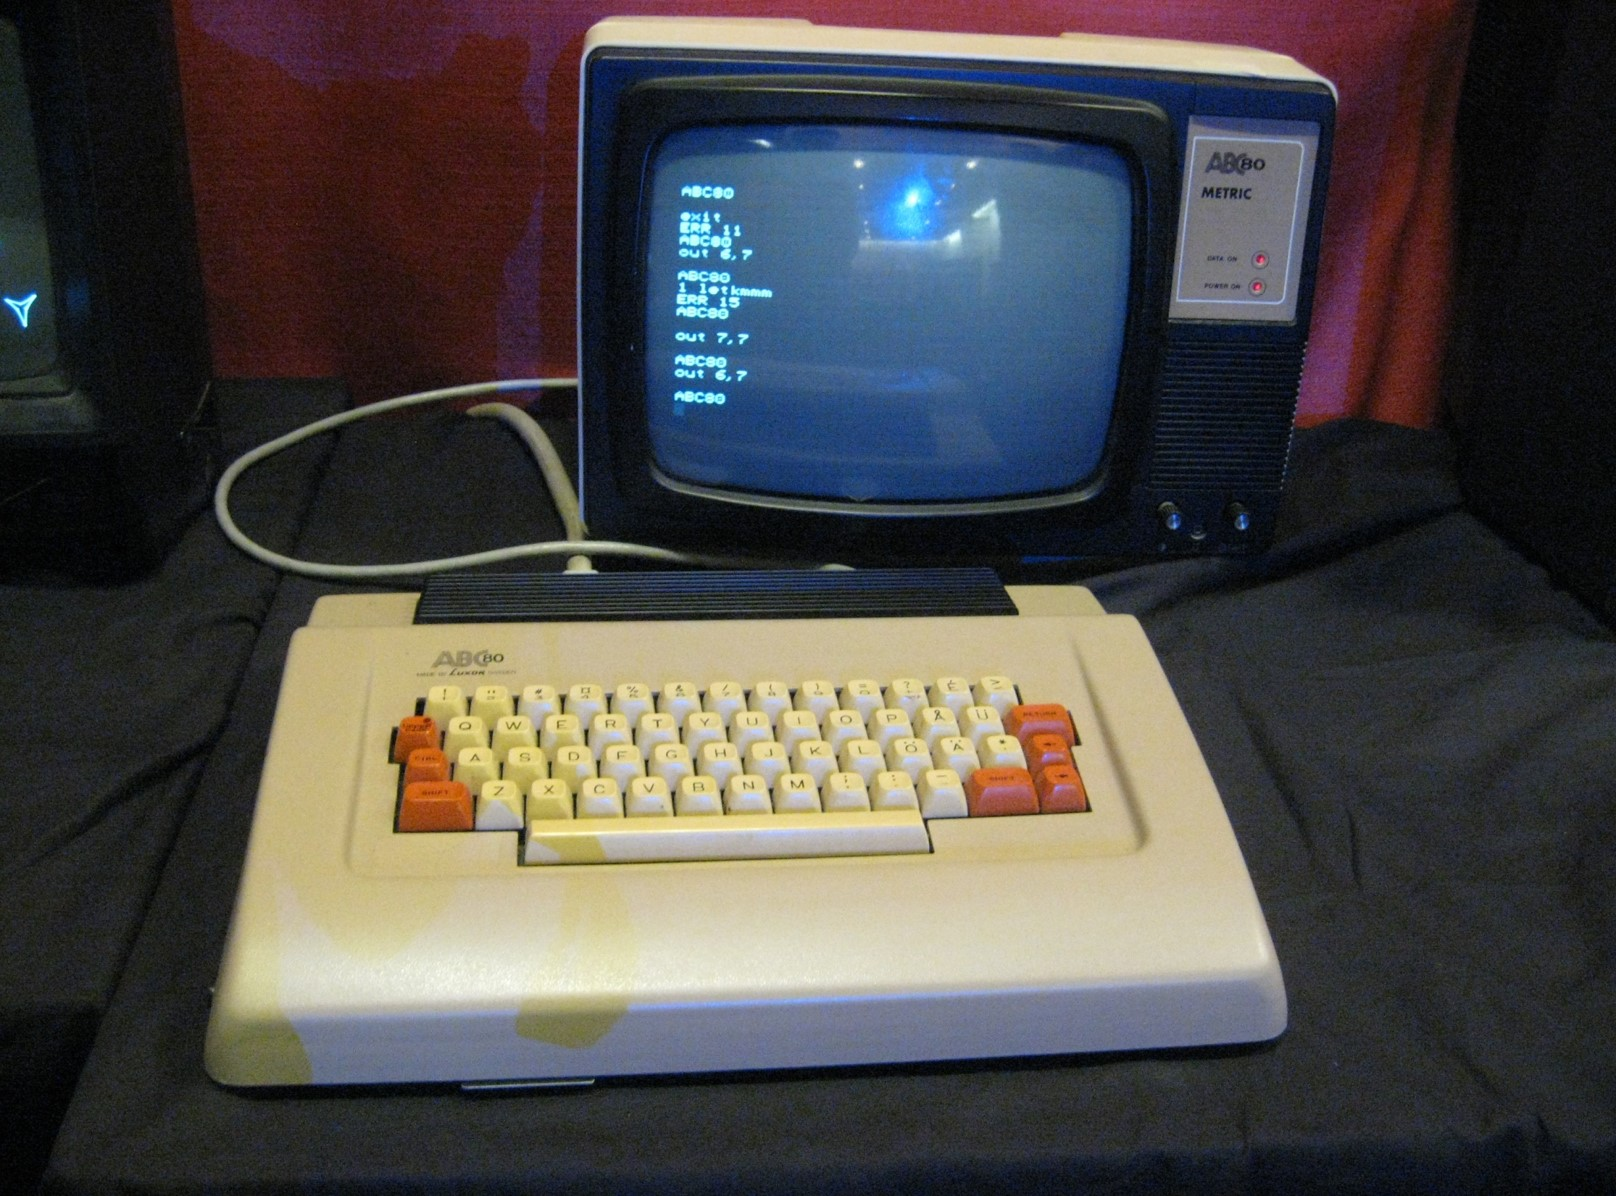
\includegraphics[width=0.8\textwidth]{../img/abc80.jpg}
\end{column}
\begin{column}{0.3\textwidth}
\pause
\begin{verbatim}
hej
hej
hej
hej
hej
hej
hej
hej
hej
hej
hej
hej
<Ctrl+C>
\end{verbatim}

\end{column}
\end{columns}
\end{Slide}


\begin{Slide}{Loopa genom elementen i en vektor}
En \code{for}-\Emph{sats} som skriver ut alla element i en vektor:
\begin{REPL}
scala> val grönsaker = Vector("gurka","tomat","paprika","selleri")

scala> for (g <- grönsaker) println(g)
gurka
tomat
paprika
selleri

\end{REPL}

\end{Slide}


\begin{Slide}{Bygga en ny samling från en befintlig med for-uttryck}
Ett \code{for}-\code{yield}-\Emph{uttryck} som \Emph{skapar en \Alert{ny} samling}.

\begin{Code}[basicstyle=\ttfamily\fontsize{12}{14}\selectfont]
for (g <- grönsaker) yield "god " + g
\end{Code}

\begin{REPL}
scala> val grönsaker = Vector("gurka","tomat","paprika","selleri")

scala> for (g <- grönsaker) yield "god " + g
res0: scala.collection.immutable.Vector[String] = 
  Vector(god gurka, god tomat, god paprika, god selleri)

scala> val åsikter = for (g <- grönsaker) yield s"god $g"
åsikter: scala.collection.immutable.Vector[String] = 
  Vector(god gurka, god tomat, god paprika, god selleri)
\end{REPL}

\end{Slide}


\begin{Slide}{Samlingen \code{Range} håller reda på intervall}
\begin{itemize}
\item Med en \code{Range(start, slut)} kan du skapa ett intervall: \\ från och med \code{start} till (men inte med) \code{slut}
\end{itemize}

\begin{REPLnonum}
scala> Range(0, 42)
res0: scala.collection.immutable.Range = 
  Range(0, 1, 2, 3, 4, 5, 6, 7, 8, 9, 10, 11, 12, 13, 14, 
    15, 16, 17, 18, 19, 20, 21, 22, 23, 24, 25, 26, 27, 28, 
    29, 30, 31, 32, 33, 34, 35, 36, 37, 38, 39, 40, 41)
\end{REPLnonum}

\begin{itemize}
\item Men alla värden däremellan skapas inte förrän de behövs:
\end{itemize}

\begin{REPL}
scala> val jättestortIntervall = Range(0, Int.MaxValue)
jättestortIntervall: scala.collection.immutable.Range = Range(0, 1, 2, 3, 4, 5, ...

scala> jättestortIntervall.end
res1: Int = 2147483647

scala> jättestortIntervall.toVector
java.lang.OutOfMemoryError: GC overhead limit exceeded
\end{REPL}

\end{Slide}

\begin{Slide}{Loopa med Range}
\code{Range} används i for-lopar för att hålla reda på antalet rundor.
\begin{REPLnonum}
scala> for (i <- Range(0, 6)) print(" gurka " + i)
 gurka 0 gurka 1 gurka 2 gurka 3 gurka 4 gurka 5 
\end{REPLnonum}
Du kan skapa en \code{Range} med \code{until} efter ett heltal:
\begin{REPLnonum}
scala> 1 until 7
res1: scala.collection.immutable.Range = 
  Range(1, 2, 3, 4, 5, 6)

scala> for (i <- 1 until 7) print(" tomat " + i) 
 tomat 1 tomat 2 tomat 3 tomat 4 tomat 5 tomat 6

\end{REPLnonum}
\end{Slide}

\begin{Slide}{Loopa med Range skapad med \texttt{to}}

Med \code{to} efter ett heltal får du en \code{Range} till och \Emph{med} sista:
\begin{REPLnonum}
scala> 1 to 6
res2: scala.collection.immutable.Range.Inclusive = 
  Range(1, 2, 3, 4, 5, 6)

scala> for (i <- 1 to 6) print(" gurka " + i) 
 gurka 1 gurka 2 gurka 3 gurka 4 gurka 5 gurka 6
 
\end{REPLnonum}


\end{Slide}



\begin{Slide}{Vad är en \code{Array} i JVM?}


\begin{itemize}
\item En \code{Array} liknar en \code{Vector} men har en särställning i JVM:
\begin{itemize}
\item Lagras som en sekvens i minnet på efterföljande adresser.
\item \Emph{Fördel}: snabbaste samlingen för element-access i JVM.
\item Men det finns en hel del \Alert{nackdelar} som vi ska se senare.
\end{itemize}

\end{itemize}

\begin{REPLnonum}
scala> val heltal = Array(42, 13, -1, 0 , 1)
\end{REPLnonum}

\begin{tikzpicture}[font=\ttfamily,scale=0.75, every node/.style={scale=0.75}]
\matrix [matrix of nodes, row sep=0, column 2/.style={nodes={rectangle,draw,minimum width=3em}}] (var) at (0cm, 2.8cm)
{
heltal   &  \makebox(16,12){ }\\
};
\matrix [matrix of nodes, draw=black,row sep=0, column 2/.style={nodes={rectangle,draw,minimum width=4em}}] (vec) at (4cm, 1cm)
{
\textit{plats} &  \\
0   &  \makebox(16,12){42}\\
1   &  \makebox(16,12){13}\\
2   &  \makebox(16,12){-1}\\
3   &  \makebox(16,12){0}\\
4   &  \makebox(16,12){1}\\
};
\filldraw[black] (0.7cm,2.8cm) circle (3pt) node[] (ref) {};
 \draw [arrow] (ref) -- (vec);
\end{tikzpicture}
\end{Slide}

\begin{Slide}{Några likheter \& skillnader mellan \texttt{Vector} och \texttt{Array}}\SlideFontSmall
\begin{multicols}{2}
\begin{REPL}[numbers=none]
scala> val xs = Vector(1,2,3)
\end{REPL}

\columnbreak

\begin{REPL}[numbers=none]
scala> val xs = Array(1,2,3)
\end{REPL}
\end{multicols}


Några likheter mellan \texttt{Vector} och \texttt{Array}
\begin{itemize}
\item Båda är samlingar som kan innehålla många element.

\item Med båda kan man snabbt accessa vilket element som helst: \code{xs(2)}

\item Båda har en fix storlek efter allokering.
\end{itemize}

Några viktiga skillnader:
\begin{multicols}{2}
\Emph{Vector}
\begin{itemize}
\item Är \Emph{oföränderlig}: du kan lita på att elementreferenserna aldrig någonsin kommer att ändras.

\item Är \Emph{snabb på att skapa en delvis förändrad kopia}, t.ex. tillägg/borttagning/uppdatering mitt i sekvensen.

\end{itemize}


\columnbreak

\Alert{Array}
\begin{itemize}
\item Är \Alert{föränderlig}: \code{xs(2) = 42}

\item Är \Alert{snabb} om man bara vill läsa eller skriva på befintliga platser.

\item Är \Alert{långsam} om man vill lägga till eller ta bort element mitt i sekvensen.

\end{itemize}
\end{multicols}
\end{Slide}



\Subsection{Huvudprogram med \texttt{main} i Scala och Java}

\begin{Slide}{Ett minimalt fristående program i Scala och Java}
Nedan Scala-kod skrivs i en editor, spara med valfritt filnamn:
\begin{Code}
// this is Scala 

object Hello {
  def main(args: Array[String]): Unit = {
    println("Hejsan scala-appen!")
  }
}
\end{Code}

\pause
\vspace{1em}
Nedan Java-kod skrivs i en editor, filen \Alert{måste} heta \texttt{Hi.java}

\begin{Code}[language=Java]
// this is Java 

public class Hi {
    public static void main(String[] args) {
        System.out.println("Hejsan Java-appen!");
    }
}
\end{Code}

\end{Slide}


\begin{Slide}{Loopa genom en samling med en \texttt{while}-sats}
\begin{REPLnonum}
scala> val xs = Vector("Hej","på","dej","!!!")
xs: scala.collection.immutable.Vector[String] = 
  Vector(Hej, på, dej, !!!)

scala> xs.size
res0: Int = 4

scala> var i = 0
i: Int = 0

scala> while (i < xs.size) { println(xs(i)); i = i + 1 }
Hej
på
dej
!!!
\end{REPLnonum}
\end{Slide}


\begin{Slide}{Loopa genom argumenten i ett Scala-huvudprogram}
Skriv denna kod och spara i filen \texttt{helloargs.scala}
\begin{REPL}[numbers=none]
$ gedit helloargs.scala
\end{REPL}
\begin{Code}
object HelloScalaArgs {
  def main(args: Array[String]): Unit = {
    var i = 0
    while (i < args.size) { 
      println(args(i))
      i = i + 1
    }
  }
}
\end{Code}
Kompilera och kör:
\begin{REPL}
$ scalac helloargs.scala
$ scala HelloScalaArgs hej gurka tomat 
hej
gurka
tomat
\end{REPL}
\end{Slide}


\begin{Slide}{Loopa genom argumenten i ett Java-huvudprogram}
\begin{REPL}[numbers=none]
$ gedit HelloJavaArgs.java
\end{REPL}
\begin{Code}[language=Java]
// this is Java 

public class HelloJavaArgs {
    public static void main(String[] args) {
    int i = 0;
    while (i < args.length) { 
      System.out.println(args[i]);
      i = i + 1;
    }
  }
}
\end{Code}
Kompilera och kör:
\begin{REPL}
$ javac HelloJavaArgs.scala
$ java HelloJavaArgs hej gurka tomat 
hej
gurka
tomat
\end{REPL}

\end{Slide}


\begin{Slide}{Scala-skript}
\begin{itemize}
\item Skala-kod kan köras som ett \Emph{skript}.\footnote{\SlideFontTiny Du får prova detta på övningen. Vi kommer mest att köra kompilerat i kursen, då Scala-skript saknar mekanism för inkludering av andra skript. Men det finns ett öppenkällkodsprojekt som löser det: \url{http://www.lihaoyi.com/Ammonite/}
}
\item Ett skript kompileras varje gång innan det körs och maskinkoden sparas inte som vid vanlig kompilering.
\item Då behövs ingen \code{main} och inget \code{object}
\end{itemize}

\begin{Code}[basicstyle=\ttfamily\fontsize{10}{12}\selectfont]
// spara nedan i filen 'myscript.scala'

println("Hejsan argumnet!")
for (arg <- args) println(arg)
\end{Code}

\begin{REPLnonum}
$ scala myscript.scala
\end{REPLnonum}


\end{Slide}



\Subsection{Algoritmer: stegvisa lösningar}

\begin{Slide}{Vad är en algoritm?}
En \href{https://sv.wikipedia.org/wiki/Algoritm}{algoritm} är en sekvens av instruktioner som beskriver \\hur man löser ett problem.\\
\vspace{1em}
\Emph{Exempel}: 
\begin{itemize}
\item	 baka en kaka 
\pause\item räkna ut din pensionsprognos 
\pause\item köra bil 
\pause\item kolla om highscore i ett spel 
\item ...
\end{itemize}

\begin{tikzpicture}[overlay]
\node[xshift=0.85\textwidth, scale=2.0] at (0,1.3) { 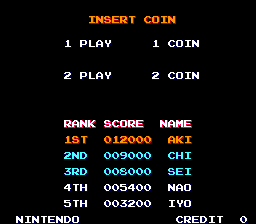
\includegraphics[width=0.25\textwidth]{../img/highscore}};
\end{tikzpicture}
\end{Slide}



\begin{Slide}{Algoritm-exempel: HIGHSCORE}
\Emph{Problem}: Kolla om high-score i ett spel \\ \vspace{1em}

\Emph{Varför?} \pause Så att de som spelar uppmuntras att spela mer :) \\ \vspace{1em}

\Emph{Algoritm:}\pause
\begin{enumerate}
\item $points$ $\leftarrow$ poängen efter senaste spelet
\item $highscore$ $\leftarrow$ bästa resultatet innan senaste spelet
\item \Key{om} $points$ är större än $highscore$ 
\begin{enumerate}[ ~~]
\item  Skriv ''Försök igen!''
\end{enumerate}
\Key{annars}
\begin{enumerate}[ ~~]
\item  Skriv ''Grattis!''
\end{enumerate}
\end{enumerate}
\pause
\scriptsize \Alert{Hittar du buggen?}
\end{Slide}


\begin{Slide}{HIGHSCORE implementerad i Scala}
\begin{Code}
import scala.io.StdIn.readLine

object HighScore {
  def main(args: Array[String]): Unit = {
    val points = readLine("Hur mång poäng fick du?").toInt
    val highscore = readLine("Vad var highscore före senaste spelet?").toInt
    val msg = if (points > highscore) "GRATTIS!" else "Försök igen!"
    println(msg) 
  }
}
\end{Code}
\pause
Är det en bugg eller en feature att det står\\ \texttt{points > highscore} \\ och inte \\ \texttt{points >= highscore} \\ ?
% Buggen är att man inte får GRATTIS om poäng == highscore vilket är tråkigt :)
\end{Slide}


\begin{Slide}{HIGHSCORE implementerad i Java}
\begin{Code}[language=Java]
import java.util.Scanner;

public class HighScore {
    public static void main(String[] args){
        Scanner scan = new Scanner(System.in);
        System.out.println("Hur många poäng fick du?");
        int points =  scan.nextInt();
        System.out.println("Vad var higscore före senaste spelet?");
        int highscore = scan.nextInt();
        if (points > highscore) {
            System.out.println("GRATTIS!");
        } else {
            System.out.println("Försök igen!");
        }
    }
}
\end{Code}
\end{Slide}


\begin{Slide}{Algoritmexempel: N-FAKULTET}
\begin{algorithm}[H]
 \SetKwInOut{Input}{Indata}\SetKwInOut{Output}{Resultat}

 \Input{heltalet $n$}
 \Output{utskrift av produkten av de första $n$ heltalen }
 ~\\
 $prod \leftarrow 1$ \\
 $i \leftarrow 2$  \\
 \While{$i \leq n$}{
  $prod \leftarrow prod * i$\\
  $i \leftarrow i + 1$
 }
 skriv ut $prod$
\end{algorithm}
\pause\vspace{1em}
\begin{itemize}\SlideFontSmall
\item Vad händer om $n$ är noll?
\item Vad händer om $n$ är ett?
\item Vad händer om $n$ är två?
\item Vad händer om $n$ är tre?
\end{itemize}
\end{Slide}

\begin{Slide}{Algoritmexempel: MIN}
\begin{algorithm}[H]
 \SetKwInOut{Input}{Indata}\SetKwInOut{Output}{Resultat}

 \Input{Array $args$ med strängar som alla innehåller heltal}
 \Output{utskrift av minsta heltalet }
 ~\\
 $min \leftarrow$ det största heltalet som kan uppkomma  \\
 $n \leftarrow $ antalet heltal \\
 $i \leftarrow 0$ \\
 \While{$i < n$}{
   $x \leftarrow args(i).toInt$ \\
   \If{( x < $min$)}{$min \leftarrow x$}
   $i \leftarrow i + 1$
 }
 skriv ut $min$
\end{algorithm}
\pause{\hfill \SlideFontTiny \Emph{Test med indata}: \code{args = Array("2", "42", "1", "2")}}
\end{Slide}


\Subsection{Funktioner skapar struktur}

\begin{Slide}{Mall för funktionsdefinitioner}

\code{def} funktionsnamn(parameterdeklarationer): returtyp = block

\pause\vspace{0.5em}\Emph{Exempel}:

\begin{Code}[basicstyle=\ttfamily\fontsize{9}{11}\selectfont]
def öka(i: Int): Int = { i + 1 }
\end{Code}
\pause Om ett enda uttryck: behövs inga \code|{}|. Returtypen kan härledas.
\begin{Code}[basicstyle=\ttfamily\fontsize{9}{11}\selectfont]
def öka(i: Int) = i + 1  
\end{Code}
\pause Om flera parametrar, separera dem med kommatecken: 
\begin{Code}[basicstyle=\ttfamily\fontsize{9}{11}\selectfont]
def isHighscore(points: Int, high: Int): Boolean = {
  val highscore: Boolean = points > high
  if (highscore) println(":)") else print(":(")
  highscore
}
\end{Code}
\pause Ovan funktion har \Alert{sidoeffekten} att skriva ut en smiley.
\end{Slide}

\begin{Slide}{Bättre många små abstraktioner som gör en sak var}

\begin{Code}[basicstyle=\ttfamily\fontsize{8}{11}\selectfont]
def isHighscore(points: Int, high: Int): Boolean = points > high

def printSmiley(isHappy: Boolean): Unit = 
  if (isHappy) println(":)") else print(":(")
\end{Code}

\pause\vspace{2em}
\begin{REPLnonum}
  printSmiley(isHighscore(113,99))
\end{REPLnonum}

\pause\vspace{2em} \code{isHigscore} är en \Emph{äkta funktion} som alltid ger samma svar för samma inparametrar och saknar \Alert{sidoeffekter}.

\end{Slide}



\begin{Slide}{Vad är ett block?}

\begin{itemize}
\item Ett block \Emph{kapslar in} flera satser/uttryck och ser ''utifrån'' ut som en enda sats/uttryck.

\item Ett block skapas med hjälp av klammerparenteser (''krullparenteser'')

\item [] {\fontsize{14}{18}\selectfont \code|{ uttryck1; uttryck2; ... uttryckN }|}\\~

\pause

\item I Scala (till skillnad från många andra språk) har ett block ett \Emph{värde} och är alltså ett \Emph{uttryck}. 

\item Värdet ges av \Emph{sista uttrycket}.

\begin{REPLnonum}
scala> val x = { println(1 + 1); println(2 + 2); 3 + 3 } 
2
4
x: Int = 6
\end{REPLnonum}


\end{itemize}

\end{Slide}

\begin{Slide}{Namn i block blir \textbf{lokala}}
Synlighetsregler: 
\begin{enumerate}
\item Identifierare deklarerade inuti ett block blir \Emph{lokala}.

\item Lokala namn \Alert{överskuggar} namn i yttre block om samma.


\item Namn syns i nästlade underblock.

\end{enumerate}

\begin{REPL}
scala> { val lokaltNamn = 42; println(lokaltNamn) }
42

scala> println(lokaltNamn)
<console>:12: error: not found: value lokaltNamn
       println(lokaltNamn)

scala> { val x = 42; { val x = 76; println(x) }; println(x) }
76
42

scala> { val x = 42; { val y = x + 1; println(y) } }
43
\end{REPL}

\end{Slide}


\begin{Slide}{Parameter och argument}

Skilj på parameter och argument!
\begin{itemize}
\item En \Alert{parameter} är det deklarerade namnet som används \Alert{lokalt} i en funktion för att referera till...

\item \Emph{argumentet} som är värdet som skickas med \Emph{vid anrop} och binds till det lokala parameternamnet.

\end{itemize}


\begin{REPLnonum}
scala> val ettArgument = 42

scala> def öka(minParameter: Int) = minParameter + 1

scala> öka(ettArgument)
\end{REPLnonum}


Speciell syntax: anrop med s.k. \Emph{namngiven parameter}
\begin{REPLnonum}
scala> öka(minParameter = ettArgument) 
\end{REPLnonum}

\end{Slide}

\begin{Slide}{Procedurer}\SlideFontSmall
\begin{itemize}
\item En \Emph{procedur} är en funktion som \Alert{gör} något intressant, men som \Alert{inte} lämnar något intressant returvärde.
\item Exempel på befintlig procedur: \code{println("hej")}
\item Du \Emph{deklarerar egna procedurer} genom att ange \texttt{\Alert{Unit}} som returvärdestyp. Då ges värdet \texttt{\Alert{()}} som betyder ''inget''.
\end{itemize}
\begin{REPL}
scala> def hej(x: String): Unit = println(s"Hej på dej $x!")
hej: (x: String)Unit

scala> hej("Herr Gurka")
Hej på dej Herr Gurka!

scala> val x = hej("Fru Tomat")
Hej på dej Fru Tomat!
x: Unit = ()
\end{REPL}
\begin{itemize}
\item Det som \Alert{görs} kallas (sido)\Emph{effekt}. Ovan är utskriften själva effekten.
\item Funktioner kan också ha sidoeffekter. De kallas då \Alert{oäkta} funktioner.
\end{itemize}
\end{Slide}

\begin{Slide}{''Ingenting'' \emph{är} faktiskt någonting i Scala}
\begin{itemize}
\item I många språk (Java, C, C++, ...) är funktioner som saknar värden speciella.
 Java m.fl. har speciell syntax för procedurer med nyckelordet \jcode{void}, men \Alert{inte} Scala. 

\item I Scala är procedurer inte specialfall; de är vanliga funktioner som returnerar ett värde som \Emph{representerar} ingenting, nämligen () som är av typen Unit. 

\item På så sätt blir procedurer inget undantag utan följer vanlig syntax och semantik precis som för alla andra funktioner.

\item Detta är typiskt för Scala: generalisera koncepten och vi slipper besvärliga undantag! \\(Men vi måste förstå generaliseringen...)


\item [] {\SlideFontSmall 
\url{https://en.wikipedia.org/wiki/Void_type}
\url{https://en.wikipedia.org/wiki/Unit_type}
}

\end{itemize}

\end{Slide}

\begin{Slide}{Abstraktion: Problemlösning genom nedbrytning i enkla funktioner och procedurer som kombineras}\SlideFontSmall
\begin{itemize}
\item En av de allra viktigaste principerna inom programmering är \Emph{funktionell nedbrytning} där  \Emph{underprogram} i form av funktioner och procedurer skapas för att bli byggstenar som kombineras till mer avancerade funktioner och procedurer.

\item Genom de namn som definieras skapas \Emph{återanvändbara abstraktioner} som kapslar in det funktionen gör. 

\item Problemet blir med bra byggblock lättare att lösa.

\item Abstraktioner som beräknar eller gör \Emph{en enda, väldefinierad sak} är enklare att använda, jämfört med de som gör många, helt olika saker.

\item Abstraktioner med \Emph{välgenomtänkta namn} är enklare att använda, jämfört med kryptiska eller missvisande namn.
\end{itemize}

\end{Slide}



\begin{Slide}{Exempel på \textbf{funktionell nedbrytning}}

Kojo-labben gav exempel på \Emph{funktionell nedbrytning} där ett antal abstraktioner skapas och återanvänds.

\begin{Code}
// skapa abstraktioner som bygger på varandra

def kvadrat = upprepa(4){fram; höger}

def stapel = {
  upprepa(10){kvadrat; hoppa}
  hoppa(-10*25)
}

def rutnät = upprepa(10){stapel; höger; fram; vänster}

// huvudprogram 

sudda; sakta(200)
rutnät
\end{Code}
\end{Slide}


\begin{Slide}{Varför abstraktion?}
\begin{itemize}
\item Stora program behöver delas upp annars blir det mycket svårt att förstå och bygga vidare på programmet.
\item Vi behöver kunna välja namn på saker i koden \textit{lokalt}, utan att det krockar med samma namn i andra delar av koden.
\item Abstraktioner hjälper till att hantera och kapsla in komplexa delar så att de blir enklare att använda om och om igen. 

\item Exempel på \Emph{abstraktionsmekanismer} i Scala och Java:
\begin{itemize}

\item \href{https://sv.wikipedia.org/wiki/Klass_\%28programmering\%29}{Klasser} är ''byggblock'' med kod som används för att skapa \href{https://sv.wikipedia.org/wiki/Objektorienterad_programmering\#Objekt}{objekt}, innehållande delar som hör ihop. \\ Nyckelord: \code{class} och \code{object} 

\item \href{https://en.wikipedia.org/wiki/Method_\%28computer_programming\%29}{Metoder} är funktioner som finns i klasser/objekt och används för att lösa specifika uppgifter.  Nyckelord: \code{def}

\item \href{https://en.wikipedia.org/wiki/Java_package}{Paket} används för att organisera kodfiler i en hierarkisk katalogstruktur och skapa namnrymder. \\Nyckelord: \Key{package}

\end{itemize}

\end{itemize}
\end{Slide}


\Subsection{Katalogstruktur för kodfiler med paket}



\begin{Slide}{Källkodsfiler och klassfiler}
\begin{tikzpicture}[node distance=1.5cm]
\node (input) [startstop] {\texttt{Hello.scala}};
\node(inptext) [right of=input, text width=5cm, scale=1.2,xshift=3.5cm]{Källkodsfil};
\node (compile) [process, below of=input] {\texttt{scalac}};
\node (output) [startstop, below of=compile] {\texttt{Hello.class}};
\node(outtext) [right of=output, text width=5cm, scale=1.2,xshift=3.5cm]{\texttt{.class}-fil med byte-kod};
\node (jvm) [process, below of=output] {JVM};
\node(jvmtext) [right of=jvm, text width=5.5cm, scale=0.8,xshift=4.5cm]{\textit{Java Virtual Machine}\\Översätter till maskinkod\\ som passar din specifika CPU\\medan programmet kör};
\draw [arrow] (input) -- (compile);
\draw [arrow] (compile) -- (output);
\draw [arrow] (output) -- (jvm);
\end{tikzpicture}
\end{Slide}




\begin{Slide}{Paket}\SlideFontSmall
\begin{itemize}
\item Paket ger struktur åt kodfilerna. Bra om man har många kodfiler.

\item Byte-koden placeras av kompilatorn i kataloger enligt paketstrukturen.


\end{itemize}

\vspace{1em}
\begin{tikzpicture}[node distance=1.5cm,scale=0.8, every node/.style={transform shape}]
\node (input) [startstop] {\texttt{greeting/Hello.scala}};
\node(inptext) [right of=input, text width=4cm, scale=1.2,xshift=4.5cm]{\lstinline{package greeting}\\\lstinline{object Hello { ... }};
\node (compile) [process, below of=input] {\texttt{scalac  greeting/Hello.java}};
\node (output) [startstop, below of=compile] {\texttt{greeting/Hello.class}};
\node(outtext) [right of=output, text width=4cm, scale=1.2,xshift=4.5cm]{Paketens bytekod hamnar i katalog med samma namn som paketnamnet};
\node (jvm) [process, below of=output] {\texttt{scala greeting.Hello}};
\draw [arrow] (input) -- (compile);
\draw [arrow] (compile) -- (output);
\draw [arrow] (output) -- (jvm);
\end{tikzpicture}

{\SlideFontTiny\vspace{1em} Katalogstrukturen för källkoden måste i Java motsvara paketstrukturen, \\men inte i Scala. Dock kräver många IDE att så görs även för Scala.}
\end{Slide}

\begin{Slide}{Import}
Med hjälp av punktnotation kommer man åt innehåll i ett paket.\\
\begin{Code}
val age = scala.io.StdIn.readLine("Ange din ålder:")
\end{Code}

En \code{import}-sats...
 
\begin{Code}
import scala.io.StdIn.readLine
\end{Code}

...gör så att kompilatorn ''ser'' namnet, och man slipper skriva hela sökvägen till namnet:
\begin{Code}
val age = readLine("Ange din ålder:")
\end{Code}

Man säger att det importerade namnet hamnar \Emph{\textit{in scope}}.
\end{Slide}





\begin{Slide}{Jar-filer}
\texttt{jar}-filer liknar \texttt{zip}-filer och används för att packa ihop bytekod i en enda fil för enkel distribution och körning. 

\vspace{2em}
\begin{tikzpicture}[node distance=1.5cm,scale=0.8, every node/.style={transform shape}]
\node (input) [startstop] {\texttt{greeting/}};
\node(inptext) [right of=input, text width=4cm, scale=1.2,xshift=4.5cm]{en katalog med filer};
\node (jar) [process, below of=input] 
{\texttt{jar cvf minjarfil.jar greeting}};

\node (output) [startstop, below of=compile] {\texttt{minjarfil.jar}};

\node(outtext) [right of=output, text width=4cm, scale=1.2,xshift=4.5cm]{En jar-fil med alla filer inpackade};

\node (jvm) [process, below of=output] {\texttt{scala -cp minjarfil.jar}};

\node(outtextjvm) [right of=jvm, text width=4cm, scale=1.2,xshift=4.5cm]{Lägg jar-filen till \\ ''classpath''};
\draw [arrow] (input) -- (jar);
\draw [arrow] (jar) -- (output);
\draw [arrow] (output) -- (jvm);
\end{tikzpicture}
\end{Slide}

\Subsection{Dokumentation}

\begin{Slide}{Dokumentation}\footnotesize
För att kod ska bli begriplig för människor är det bra att dokumentera vad den gör. Det finns \Emph{tre olika sorters kommentarer} som man kan skriva direkt i Scala/Java-koden, \Alert{som kompilatorn struntar fullständigt i}:
\begin{lstlisting}
// Enradskommentarer börjar med dubbla snedstreck
//       men de gäller bara till radslut

/* Flerradskommentarer börjar med 
   snedstreck-asterisk
   och slutar med asterisk-snedstreck.  */ 

/** Dokumentationskommentarer placeras före 
 *   t.ex. en funktion och berättar vad den gör
 *   och vad eventuella parametrar används till.
 *   Börjar med snedstreck-asterisk-asterisk.
 *   Varje ny kommentarsrad börjar med asterisk.
 *   Avslutas med asterisk-stjärna.
 */
\end{lstlisting}
\end{Slide}

\begin{Slide}{scaladoc}
Programmet \texttt{scaladoc}-filer läser källkod och skapar en webbsajt med dokumentation. 

\vspace{2em}
\begin{tikzpicture}[node distance=1.5cm,scale=0.8, every node/.style={transform shape}]

\node (input) [startstop] {\texttt{greeting/}};

\node(inptext) [right of=input, text width=4cm, scale=1.2,xshift=4.5cm]{en katalog med \texttt{.scala}-filer};

\node (scaladoc) [process, below of=input] 
{\texttt{scaladoc greeting/*.scala}};

\node (output) [startstop, below of=compile] {\texttt{index.html} ~~med mera...};

\node(outtext) [right of=output, text width=4cm, scale=1.2,xshift=4.5cm]{En webbsajt};


\draw [arrow] (input) -- (scaladoc);
\draw [arrow] (scaladoc) -- (output);
\end{tikzpicture}
\end{Slide}



\subsection{Att göra denna vecka}


%%%
\begin{Slide}{Att göra i Vecka \vecka: Förstå grundläggande kodstrukturer}

\begin{enumerate}
\item Laborationer är \Alert{obligatoriska}.\\ Ev. sjukdom måste anmälas \Alert{före} via mejl till kursansvarig!
\item Gör övning \texttt{programs}
\item OBS! Ingen lab denna vecka w02. Använd tiden att komma ikapp om du ligger efter!
\item Träffas i samarbetsgrupper och hjälp varandra att förstå.
\item Vi har nosat på flera koncept som vi kommer tillbaka till senare: du måste inte fatta alla detaljer redan nu.
\item Om ni inte redan gjort det: \\Visa \href{https://github.com/bjornregnell/lth-eda016-2015/tree/master/assignments}{samarbetskontrakt} för handledare på resurstid.
\item \Alert{Koda på resurstiderna} och få hjälp och tips! 
\end{enumerate}
\end{Slide}

\begin{Slide}{Veckans övning: \code{w02-programs}}\SlideFontTiny
\vspace{-0.5em}
\setlength{\leftmargini}{0pt}
\begin{itemize}
%!TEX encoding = UTF-8 Unicode
%!TEX root = ../compendium2.tex

\item Kunna skapa samlingarna Range, Array och Vector med heltals- och strängvärden.
\item Kunna indexera i en indexerbar samling, t.ex. Array och Vector.
\item Kunna anropa operationerna size, mkString, sum, min, max på samlingar som innehåller heltal.
\item Känna till grundläggande skillnader och likheter mellan samlingarna Range, Array och Vector.
\item Förstå skillnaden mellan en for-sats och ett for-uttryck.
\item Kunna skapa samlingar med heltalsvärden som resultat av enkla for-uttryck.
\item Förstå skillnaden mellan en algoritm i pseudo-kod och dess implementation.
\item Kunna implementera algoritmerna SUM, MIN/MAX på en indexerbar samling med en \code{while}-sats.
\item Kunna köra igång enkel Scala-kod i REPL, som skript och som applikation.
\item Kunna skriva och köra igång ett enkelt Java-program.
\item Känna till några grundläggande syntaxskillnader mellan Scala och Java, speciellt variabeldeklarationer och indexering i Array.
\item Förstå vad ett block och en lokal variabel är.
\item Förstå hur nästlade block påverkar namnsynlighet och namnöverskuggning.
\item Förstå kopplingen mellan paketstruktur och kodfilstruktur.
\item Kunna skapa en jar-fil.
\item Kunna skapa dokumentation med scaladoc.

\end{itemize}
\end{Slide}














%!TEX encoding = UTF-8 Unicode
%!TEX root = ../compendium1.tex

\chapter{Funktioner, Objekt}\label{chapter:W03}
Koncept du ska lära dig denna vecka:
\begin{multicols}{2}\begin{itemize}[nosep,label={$\square$},leftmargin=*]
\item definera funktion
\item anropa funktion
\item parameter
\item returtyp
\item värdeandrop
\item namnanrop
\item default-argument
\item namngivna argument
\item applicera funktion på alla element i en samling
\item procedur
\item värdeanrop vs namnanrop
\item uppdelad parameterlista
\item skapa egen kontrollstruktur
\item objekt
\item modul
\item punktnotation
\item tillstånd
\item metod
\item medlem
\item funktionsvärde
\item funktionstyp
\item äkta funktion
\item stegad funktion
\item apply
\item lazy val
\item lokala funktioner
\item aktiveringspost
\item rekursion
\item basfall
\item anropsstacken
\item objektheapen
\item cslib.window.SimpleWindow\end{itemize}\end{multicols}


%!TEX encoding = UTF-8 Unicode
%!TEX root = ../lect-w03.tex


% \ifkompendium\else
% \Subsection{Scala 2.12.10}

% \begin{SlideExtra}{Scala 2.12.10}
%   Den 10:e September släpptes Scala 2.12.10 med viktigaste förbättringen att filtrering i Scaladoc nu fungerar igen. 
%   \\~\\
%   \url{https://www.scala-lang.org/news/2.12.10}
%   \\~\\ Du kan gärna installera 2.12.10 om du vill, men inte nödvändigt.
%   \\~\\ När du kollar api-dokumentationen för Scalas standardbibliotek så använd denna länk:\\ 
%   \url{https://www.scala-lang.org/api/2.12.10}

% \end{SlideExtra}
% \fi

\Subsection{Vad är en funktion?}


\ifkompendium\else
\begin{SlideExtra}{Om veckans tema: Funktioner}
\begin{itemize}
  \item Funktioner är en av de viktigaste abstraktionsmekanismerna inom datavetenskapen
  \item Du kan redan massor om funktioner, bl.a. från matematiken.
  \item Denna vecka ska vi fördjupa förståelsen:
  \begin{itemize}\SlideFontSize{6}{8}
    \item överlagring
    \item enhetlig access
    \item defaultargument
    \item namngivna argument
    \item lokala funktioner
    \item funktioner som äkta värden
    \item anonyma funktioner
    \item klammerparentes vid ensam paramenter
    \item multipla parameterlistor
    \item egendefinierade kontrollstrukturer
    \item fördröjd evaluering (''call-by-name'')
    \item stegade funktioner (''Curry-funktioner'')
    \item fångad variablelrymd (''closure'')
    \end{itemize}
\end{itemize}  
\end{SlideExtra}

\begin{SlideExtra}{Om veckans tema: Funktioner}
  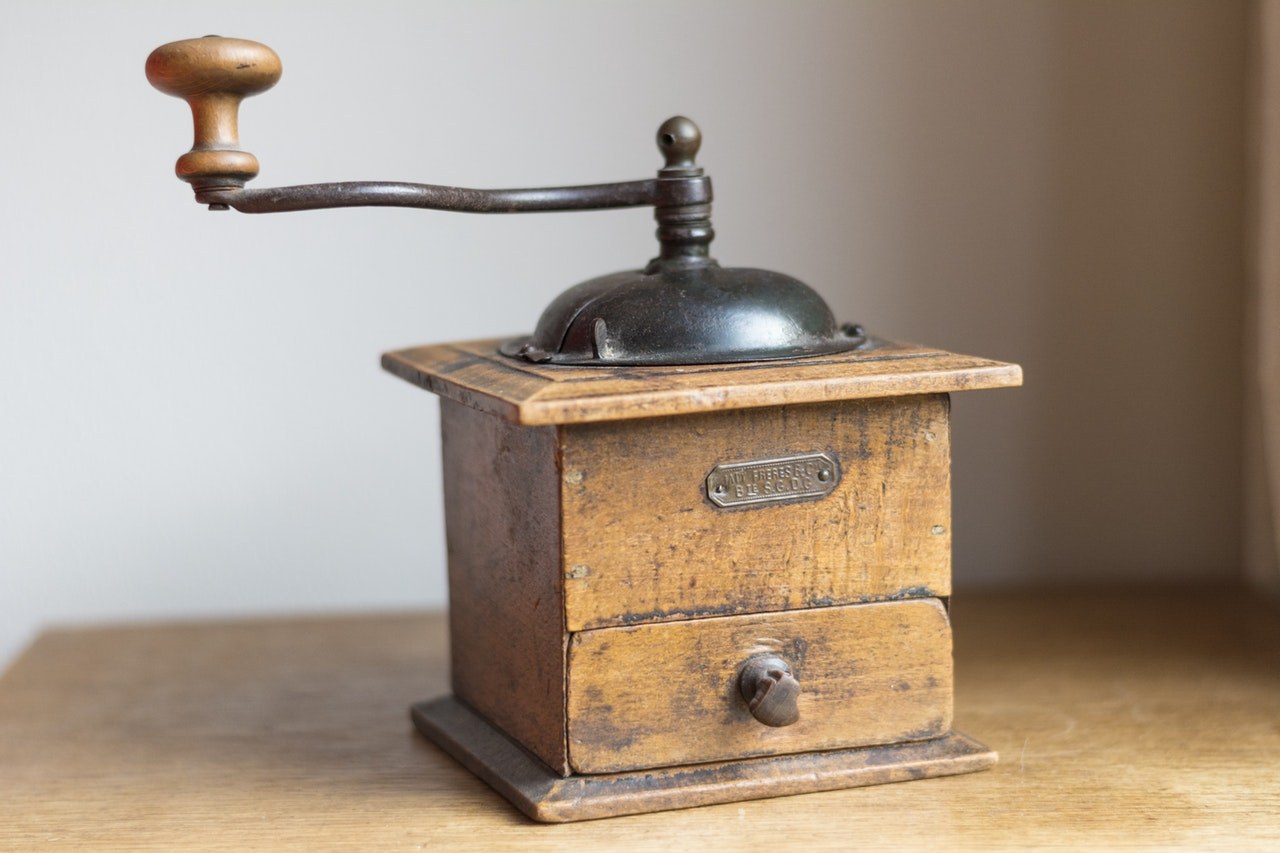
\includegraphics[width=1.0\textwidth]{../img/coffee-grinder}
\end{SlideExtra}
\fi


\begin{Slide}{Funktion: deklaration och anrop}
\SlideOnly{\setlength{\leftmargini}{0pt}}

\code{def} funktionsnamn(parameterdeklarationer): returtyp = uttryck
\vspace{0.5em}

% \begin{Code}
% def namn(param1: Typ1, param2: Typ2): Returtyp = uttryck
% \end{Code}

\begin{itemize}\SlideFontSmall
  \item En funktion har ett \Emph{huvud} och efter \code{=} kommer dess \Emph{kropp}.
  \item En \Alert{namngiven} funktion \Emph{deklareras} med nyckelordet \code{def}
  \item En funktion kan ha \Emph{parametrar} som deklareras i huvudet. 
  \item Kroppen ska vara ett uttryck (ev. ett block med flera uttryck).
  \item Parametrar binds till argument vid anrop.
  \item Uttrycket i funktionens kropp \Emph{evalueras} vid \Alert{varje anrop}. 
  \item Värdet av uttrycket blir funktionen \Emph{returvärde}. 
\end{itemize}

\pause
Exempel:
\begin{Code}
def öka(a: Int, b: Int): Int = a + b
\end{Code}
\pause
\begin{REPLnonum}
scala> öka(42, 1)
val res0: Int = 43
\end{REPLnonum}

\end{Slide}


\begin{Slide}{Deklarera funktioner, överlagring}
\begin{itemize}
\item En parameter, och sedan två parametrar:
\begin{REPL}
scala> def öka(a: Int): Int = a + 1

scala> def öka(a: Int, b: Int): Int = a + b

scala> öka(1)
val res0: Int = 2

scala> öka(1,1)
val res1: Int = 2

\end{REPL}
\item Båda funktionerna ovan kan finnas samtidigt! Trots att de har \Emph{samma namn} är de \Alert{olika funktioner}; kompilatorn kan skilja dem åt med hjälp av de \Alert{olika parameterlistorna}.

\item Detta kallas \Emph{överlagring} \Eng{overloading} av funktioner.
\item Överlagring ger flexibilitet i användningen; vi slipper hitta på nytt namn så som \code{öka2} vid 2 parametrar.
\end{itemize}
\end{Slide}



\begin{Slide}{Funktioner med defaultargument}\SlideFontSmall

\begin{itemize}
\item Vi kan ofta åstadkomma samma flexibilitet som vid överlagring, men med \Alert{en enda} funktion, om vi i stället använder \Emph{defaultargument}:
\begin{REPLnonum}
scala> def inc(a: Int, b: Int = 1) = a + b

scala> inc(42, 2)
val res0: Int = 44

scala> inc(42, 1)
val res1: Int = 43

scala> inc(42)
val res2: Int = 43

\end{REPLnonum}
\item Om ett argument utelämnas och parametern deklarerats med defaultargument så appliceras detta. Kompilatorn fyller alltså i argumentet åt oss, om det är entydigt vilken parameter som avses.
\end{itemize}
\end{Slide}


\begin{Slide}{Funktioner med namngivna argument}
\begin{itemize}
\item Genom att använda \Emph{namngivna argument} behöver man inte hålla reda på ordningen på parametrarna, bara man känner till parameternamnen.
\item Namngivna argument går fint att \Alert{kombinera} med defaultargument.
\begin{REPLnonum}[basicstyle=\SlideFontSize{7}{9}\ttfamily\color{white}]
scala> def namn(förnamn: String,
                efternamn: String,
                förnamnFörst: Boolean = true,
                ledtext: String = "Namn:"): String =
         if förnamnFörst then s"$ledtext $förnamn $efternamn"
         else s"$ledtext $efternamn, $förnamn"

scala> namn(ledtext = "Name:", efternamn = "Coder", förnamn = "Kim")
val res0: String = Name: Kim Coder
\end{REPLnonum}
\end{itemize}
\end{Slide}


\begin{Slide}{Enhetlig access}\SlideFontSmall
\begin{itemize}
\item Om en funktion \Emph{deklareras} \Alert{med} tom parameterlista \code{()} så ska den \Emph{anropas} \Alert{med} tom parameterlista.
\begin{REPLsmall}
scala> def tomParameterlista() = 42

scala> tomParameterlista()
val res1: Int = 42

scala> tomParameterlista                                                                                                                    
1 |tomParameterlista
  |^^^^^^^^^^^^^^^^^
  |method tomParameterlista must be called with () argument
\end{REPLsmall}

\item En parameterlös funktion deklarerad \Alert{utan} \code{()} ska anropas \Alert{utan} \code{()}. 
\begin{REPLsmall}
scala> def ingenParameterlista = 42
scala> ingenParameterlista()
1 |ingenParameterlista()
  |^^^^^^^^^^^^^^^^^^^
  |method ingenParameterlista does not take parameters
\end{REPLsmall}

\item Deklaration utan \code{()} möjliggör \Emph{enhetlig access}: implementationen kan ändras från \code{val} till \code{def} eller tvärtom, \Emph{utan} att \Alert{användandet} påverkas.
\pause
%\item Om parameterlista saknas får man alltså \Alert{inte} använda \code{()} vid anrop:

\end{itemize}
\end{Slide}

\Subsection{Hur ser det ut i minnet när funktioner anropas?}

\begin{Slide}{Anropsstacken och objektheapen}\SlideFontSmall
Minnet som innehåller ett programs data är uppdelat i två delar:
\begin{itemize}
\item \Emph{Anropsstacken}: 
\begin{itemize}\SlideFontSmall
\item På stackminnet läggs en \Emph{aktiveringspost} \Eng{stack frame\footnote{\href{https://en.wikipedia.org/wiki/Call_stack}{en.wikipedia.org/wiki/Call\_stack}}, activation record} för varje funktionsanrop med plats för \Alert{parametrar} och \Alert{lokala variabler}.
\item Aktiveringsposten \Alert{raderas} när \Emph{returvärdet} har levererats.
\item Stacken \Alert{växer} vid \Emph{nästlade funktionsanrop}, då en funktion i sin tur anropar en annan funktion.
\end{itemize}
\item \Emph{Objektheapen}: I heapminnet\footnote{\href{https://en.wikipedia.org/wiki/Memory_management}{en.wikipedia.org/wiki/Memory\_management}}$^{,}$\footnote{Ej att förväxlas med datastrukturen heap  \href{https://sv.wikipedia.org/wiki/Heap}{sv.wikipedia.org/wiki/Heap}} sparas alla objekt (data) som allokeras under körning. Heapen städas då och då av \Emph{skräpsamlaren} \Eng{garbage collector}, och minne som inte används längre frigörs. \\\vspace{0.5em}
%\href{http://stackoverflow.com/questions/1565388/increase-heap-size-in-java}{stackoverflow.com/questions/1565388/increase-heap-size-in-java}
% \href{https://stackoverflow.com/questions/1441373/increase-jvm-heap-size-for-scala}{stackoverflow.com/questions/1441373/increase-jvm-heap-size-for-scala}
% \begin{REPLnonum}
% scala -J-Xmx16g -J-XX:-UseGCOverheadLimit Main
% \end{REPLnonum}
\end{itemize}
\end{Slide}

% \begin{Slide}{Aktiveringspost}\SlideFontSmall
% Nästlade anrop ger växande anropsstack.
% \begin{REPL}
% scala> def f(x: Int, y: Int): Int = { val z = x + y; println(z); z}
% scala> def g(a: Int, b: Int): Int = { val c = a + b; println(c); f(c, 2 * c) }
% scala> def h(i: Int): Int = { val n = 5; g(i, i * n) }
% scala> h(2)
% \end{REPL}
%
% \pause
% \Alert{Stacken}
%
% \begin{tabular}{|r | l | l |} \hline
%
% variabel & värde & Aktiveringspost för anrop av... \\ \hline \hline
% \pause
%  i & 2 & h \\
%  n & 5 & \\ \hline
%  \pause
%  a & 2 & g \\
%  b & 10 &  \\
%  c & 12  &  \\  \hline
%  \pause
%  x & 12  & f \\
%  y & 24 &  \\
%  z & 36 & \\ \hline
% \end{tabular}
% \end{Slide}

\begin{Slide}{Aktiveringspost}\SlideFontSmall
Nästlade anrop ger växande anropsstack.
\begin{REPLsmall}
scala> def h(x: Int, y: Int) = { val z = x + y; println(z) }

scala> def g(a: Int, b: Int) = { val x = 1; h(x + 1, a + b) }

scala> def f() = { val n = 5; g(n, 2 * n) }

scala> f()

\end{REPLsmall}

\pause
\Alert{Stacken}

\begin{tabular}{|r | l | l |} \hline

variabel & värde & Aktiveringspost för anrop av... \\ \hline \hline
\pause
 n & 5 & f \\ \hline
 \pause
 a & 5 & g \\
 b & 10 &  \\
 x & 1  &  \\  \hline
 \pause
 x & 2  & h \\
 y & 15 &  \\
 z & 17 & \\ \hline
\end{tabular}
\end{Slide}

\begin{Slide}{Anropsstacken i Kojo Desktop}
Tryck på orange playknapp i Kojo och se anropsstacken.\vspace{0.5em}

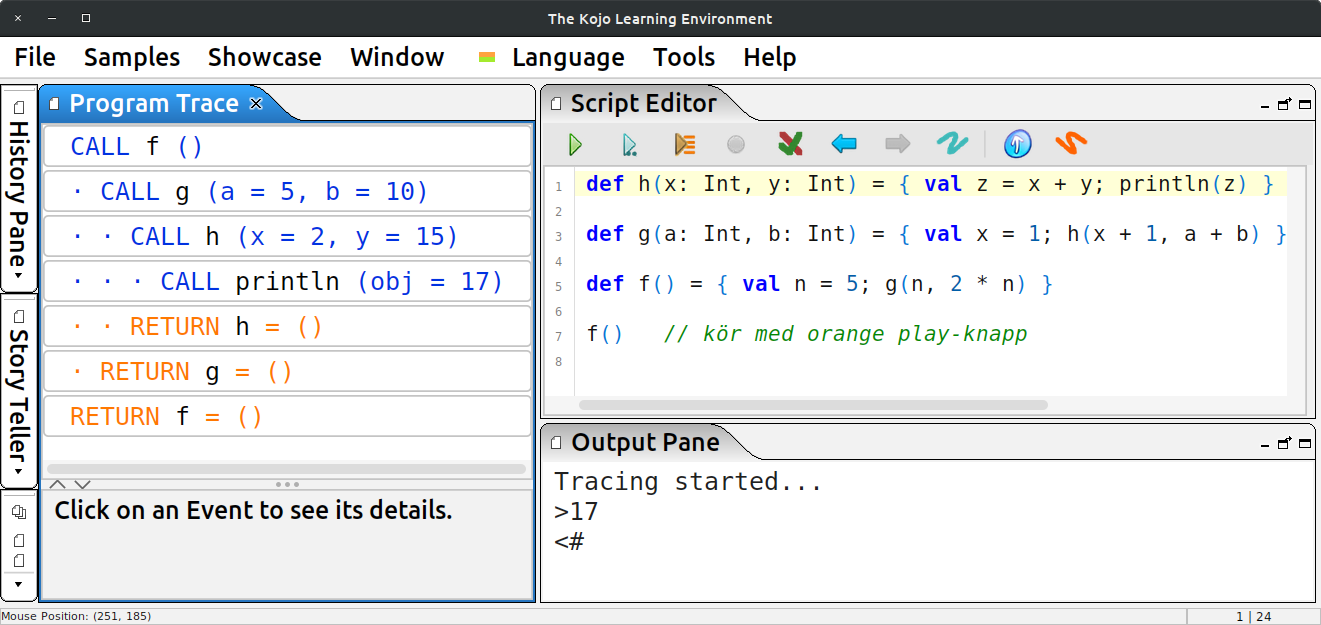
\includegraphics[width=1.0\textwidth]{../img/kojo-trace.png}  
\end{Slide}

\begin{Slide}{Anropsstacken i VS Code}
Lägg till en brytpunkt på rad 4 nedan och klicka på debug över \code{@main} i VS Code och se anropsstacken.\vspace{0.5em}

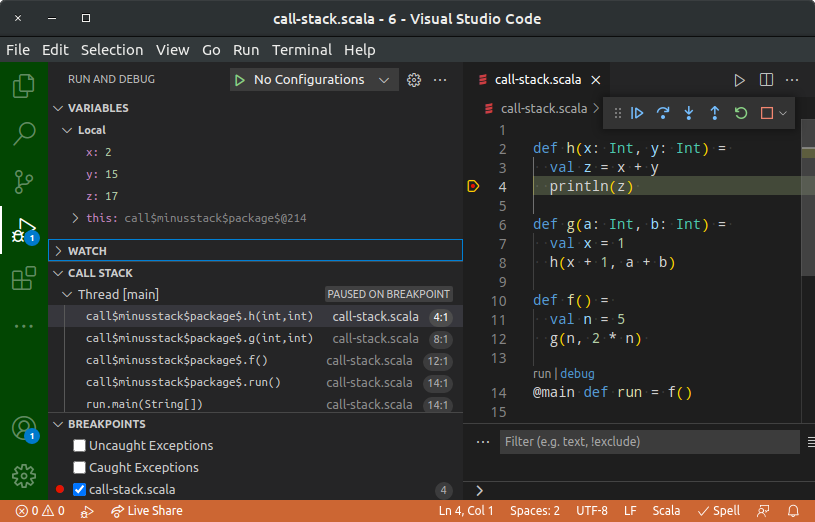
\includegraphics[width=0.85\textwidth]{../img/vscode-trace.png}  
\end{Slide}


\begin{Slide}{Vad är en stack trace?}\SlideFontSmall
När du letar buggar vid körtidsfel har du nytta av att \Alert{noga studera} \Emph{utskriften av anropsstacken} \Eng{stack trace}:
% \begin{CodeSmall}
% // Program i filen BMI.scala
% object BMI: 
%   def main(args: Array[String]): Unit = 
%     println(bmi(args(0).toInt, args(1).toInt))

%   def bmi(heightCm: Int, weightKg: Int) = 
%     safeDiv(weightKg, heightCm * heightCm) 

%   def safeDiv(numerator: Int, denominator: Int): (Int, String) = 
%     if (denominator == 0) (numerator / denominator, "ok")  // ser du buggen?
%     else (0, "division by zero") 
% \end{CodeSmall}
  
\begin{Code}[numbers=left]
// Program i filen bmi.scala

@main 
def bmi(heightCm: Int, weightKg: Int) = 
  safeDiv(weightKg, heightCm * heightCm) 

def safeDiv(numerator: Int, denominator: Int): (Int, String) = 
  if denominator == 0 then (numerator / denominator, "")  // ser du buggen?
  else (0, "division by zero")

\end{Code}
\begin{REPL}
> scalac bmi.scala 
> scala bmi 0 42
Exception in thread "main" java.lang.ArithmeticException: / by zero
        // HÄR KOMMER STACK TRACE pga körtidsfel - se nästa bild
\end{REPL}
\end{Slide}

\begin{Slide}{Hur läsa en stack trace?}
\begin{REPL}
Exception in thread "main" java.lang.ArithmeticException: / by zero
        at bmi$package$.safeDiv(bmi.scala:8)
        at bmi$package$.bmi(bmi.scala:5)
        at bmi.main(bmi.scala:3)

\end{REPL}
\begin{itemize}\SlideFontSmall
  \item En \Emph{stack trace} skrivs ut efter en krasch p.g.a. körtidsfel.
  \item Körtidsfel känns igen med ordet \Alert{Exception}.
  \item Först kommer en beskrivning av felet som orsakat kraschen, här: \\\code{java.lang.ArithmeticException: \ by zero} 
  \item Därefter visas anropsstacken.
  \item För varje funktionsanrop anges: \Emph{\texttt{klass.metod(kodfil:radnummer)}}
  \item Main-funktioner läggs i ett singelobjekt i ett speciellt paket
  \item Singelobjekt i Scala kodas som en Java-klass med dollar-tecken efter namnet, eftersom det inte finns singelobjekt i JVM.
  %\item Efter anropet av din \code{main}-procedur ligger JVM-interna anrop (\code{java.base} etc.) som du inte behöver bry dig om. %% syns inte längre i Scala 3 stack trace
\end{itemize}
\end{Slide}
  

\begin{Slide}{Lokala funktioner}\SlideFontSmall
Med lokala funktioner kan delproblem lösas med nästlade abstraktioner.

\begin{CodeSmall}
def gissaTalet(max: Int, min: Int = 1): Unit = 
  def gissat = io.StdIn.readLine(s"Gissa talet mellan $min och $max: ").toInt

  val hemlis = (math.random() * (max - min) + min).toInt

  def skrivLedtrådOmEjRätt(gissning: Int): Unit =
    if gissning > hemlis then println(s"$gissning är för stort :(")
    else if gissning < hemlis then println(s"$gissning är för litet :(")

  def inteRätt(gissning: Int): Boolean = 
    skrivLedtrådOmEjRätt(gissning)
    gissning != hemlis
  

  def loop: Int = { var i = 1; while inteRätt(gissat) do i += 1; i }

  println(s"Du hittade talet $hemlis på $loop gissningar :)")
\end{CodeSmall}

Lokala, nästlade funktionsdeklarationer är tyvärr inte tillåtna i många andra språk, t.ex. Java.\footnote{\href{http://stackoverflow.com/questions/5388584/does-java-support-inner-local-sub-methods}{\SlideFontSize{8}{9}stackoverflow.com/questions/5388584/does-java-support-inner-local-sub-methods}}

\end{Slide}

\Subsection{En funktion är ett värde}

\begin{Slide}{Funktioner är äkta värden i Scala}\SlideFontSmall
\begin{itemize}
\item En funktion är ett \Alert{äkta värde}.
\item Vi kan till exempel tilldela en variabel ett funktionsvärde.
\pause
\item Med hjälp av blank+understreck efter funktionsnamnet får vi funktionen som ett \Alert{värde} (inga argument appliceras än):
\begin{REPLnonum}
scala> def add(a: Int, b: Int) = a + b

scala> val f = add _ 
val f: (Int, Int) => Int = Lambda7210/0x0000000841e4e040@1ce2db23

scala> f(21, 21)
val res0: Int = 42
\end{REPLnonum}
\item Ett funktionsvärde har en \Alert{typ} precis som alla värden: \\
\code{f: (Int, Int) => Int}
\pause
\item Ett funktionsvärde har till skillnad från en funktionsdeklaration inget namn (variabeln \code{f} har ett namn men inte själva funktionen). Den kallas därför en \Emph{anonym} funktion eller \Alert{lambda} (mer om detta snart).
\end{itemize}
\end{Slide}

\begin{Slide}{Du kan vanligtvis skippa understreck}\SlideFontSmall
\begin{itemize}\SlideFontSmall

\item Nytt i Scala 3: Om det är otvetydigt att du vill skapa ett funktionsvärde så kan du skippa understreck:
\begin{REPLnonum}
scala> def add(a: Int, b: Int) = a + b

scala> val f = add     // inget understreck behövs 
val f: (Int, Int) => Int = Lambda7210/0x0000000841e4e040@1ce2db23
\end{REPLnonum}

\item Specialfall då understreck behövs: (se speciellt typen \code{() => Int})
\begin{REPLsmall}
scala> def a() = 42
def a(): Int

scala> val b = a
1 |val b = a
  |        ^
  |        method a must be called with () argument

scala> val b = a _
val b: () => Int = Lambda7214/0x0000000841e50440@565d794
\end{REPLsmall}
\item Börja utan understreck och se om det funkar utan kompileringsfel...
\end{itemize}
\end{Slide}

\begin{Slide}{Funktionsvärden kan vara argument}
En funktion kan ha en annan funktion som parameter:
\begin{REPL}
scala> def tvåGånger(x: Int, f: Int => Int) = f(f(x))

scala> def öka(x: Int) = x + 1

scala> def minska(x: Int) = x - 1

scala> tvåGånger(42, öka)
val res1: Int = 44

scala> tvåGånger(42, minska)
val res1: Int = 40
\end{REPL}
\end{Slide}



\begin{Slide}{Applicera funktioner på element i samlingar med \texttt{map}}\SlideFontSmall
\begin{Code}
def öka(x: Int) = x + 1

def minska(x: Int) = x - 1

val xs = Vector(1, 2, 3)
\end{Code}
\pause
Metoden \Emph{\texttt{map}} fungerar på alla Scala-samlingar och tar \Emph{en funktion som argument} och applicerar denna funktion på alla element och \Alert{skapar en ny samling} med resultaten:
\begin{REPL}
scala> xs.map(öka)
val res0: ???   // vad blir resultatet?

scala> xs.map(minska)
val res1: ???   // vad blir resultatet?
\end{REPL}
En funktion som har funktionsvärden som indata (eller utdata) kallas en\\ \Emph{högre ordningens funktion}  \Eng{higher-order function}.
\end{Slide}


\begin{Slide}{Applicera funktioner på element i samlingar med \texttt{map}}\SlideFontSmall
\begin{Code}
def öka(x: Int) = x + 1

def minska(x: Int) = x - 1

val xs = Vector(1, 2, 3)
\end{Code}
Metoden \Emph{\texttt{map}} fungerar på alla Scala-samlingar och tar \Emph{en funktion som argument} och applicerar denna funktion på alla element och \Alert{skapar en ny samling} med resultaten:
\begin{REPL}
scala> xs.map(öka)
val res0: scala.collection.immutable.Vector[Int] = Vector(2, 3, 4)

scala> xs.map(minska)
val res1: scala.collection.immutable.Vector[Int] = Vector(0, 1, 2)
\end{REPL}
En funktion som har funktionsvärden som indata kallas en\\ \Emph{högre ordningens funktion}  \Eng{higher-order function}.
\end{Slide}

\Subsection{Äkta funktioner}

\begin{Slide}{Äkta funktioner}
\begin{itemize}\SlideFontSmall
\item En \Emph{äkta} \Eng{pure} funktion är en funktion som ger ett resultat som \Alert{enbart} beror av dess argument. Alltså som funktioner i matematiken.
\item En äkta (matematisk) funktion är \Emph{referentiellt transparent} \Eng{referentially transparent}, vilket innebär att varje anrop kan bytas ut mot funktionskroppen där parametrarna ersatts med motsvarande argument.
\item En äkta funktion har \Alert{inga sidoeffekter}, t.ex. utskrift, skriva/läsa filer,  eller uppdateringar av variabler \Alert{synliga utanför} funktionen.
\item Exempel:
\begin{Code}
def add(x: Int, y: Int): Int = x + y              // äkta funktion
def rnd(n: Int): Int = (math.random() * n).toInt  // oäkta funktion
\end{Code} 
\begin{itemize}\SlideFontTiny

\item Uttrycket \code{add(41, 1)} kan ersättas med 41 +1 som i sin tur kan ersättas med 42 utan att det påverkar resultatet. Resultatet av \code{add(41, 1)} blir \Emph{samma varje gång} funktionen appliceras med dessa argument
\item Uttrycket \code{rnd(42)} kan \Alert{inte} bytas ut mot ett specifikt uttryck som säkert ger samma resultat varje gång. Alltså: \emph{ej referentiell transparens}.
\end{itemize}  
\end{itemize}  
\end{Slide}

\begin{Slide}{Exempel på oäkta funktioner: slumptal}

  \begin{itemize}
    \item Funktioner vars värden på något sätt beror av slumpen är \Alert{inte} äkta funktioner.
    \item Även om samma argument ges vid upprepad applicering, så kan ju resultatet bli olika.
    \item Studera dokumentationen för \code{scala.util.Random} här:\\ \href{https://www.scala-lang.org/api/current/scala/util/Random.html}{\SlideFontSmall https://www.scala-lang.org/api/current/scala/util/Random.html}
    \item Du har nytta av funktionen \code{Random.nextInt} och slumptalsfrö \Eng{random seed} i veckans uppgifter.
  \end{itemize}

\end{Slide}

\begin{Slide}{Slumptalsfrö: få samma slumptal varje gång}\SlideFontTiny
\begin{itemize}
\item Om man använder slumptal kan det vara svårt att leta buggar, efter som det blir \Alert{olika varje gång} man kör programmet och buggen kanske bara uppstår ibland.

\item Med klassen \code{scala.util.Random} kan man skapa \Emph{pseudo}-slumptalssekvenser.
\pause
\item Om man ger ett s.k. \Emph{frö} \Eng{seed}, av heltalstyp, som argument till konstruktorn när man skapar en instans av klassen \code{scala.util.Random}, får man samma ''slumpmässiga'' sekvens \Alert{varje gång} man kör programmet.

\begin{Code}
  val seed = 42
  val rnd = util.Random(seed) // skapa ny slumpgenerator med frö 42
  val r = rnd.nextInt(6) // ger slumptal mellan 0 till och med 5
\end{Code}
\pause
\item Om man \Alert{inte} ger ett \Emph{frö} så sätts fröet till ''\emph{a value very likely to be distinct from any other invocation of this constructor}''. Då vet vi inte vilket fröet blir och det blir olika varje gång man kör programmet.
\begin{Code}
  val rnd = util.Random() // OLIKA frö varje körning
  val r = rnd.nextInt(6) // ger slumptal mellan 0 till och med 5
\end{Code}
\pause
\end{itemize}
\end{Slide}

%\begin{Slide}{Syresättning av hjärnan vid sövande föreläsning}
%Prova nedan kod som finns här:\\
%%\href{https://github.com/lunduniversity/introprog/blob/master/compendium/examples/workspace/w05-seqalg/src/NanananananananaNanananananananaBatman.scala}{\SlideFontTiny github.com/lunduniversity/introprog/.../NanananananananaNanananananananaBatman.scala} \\
%
%
%
%\vspace{0.65em}\scalainputlisting[numbers=left,numberstyle=,basicstyle=\fontsize{6.5}{8}\ttfamily\selectfont]{../compendium/examples/workspace/w05-seqalg/src/FixSleepyBrain.scala}
%
%\pause
%Medan du lyssnar till: \href{https://www.youtube.com/watch?v=zUwEIt9ez7M}{\SlideFontSmall www.youtube.com/watch?v=zUwEIt9ez7M}\\
%Eller: \href{https://www.youtube.com/watch?v=rvXxlXg_V-k}{\SlideFontSmall www.youtube.com/watch?v=rvXxlXg\_V-k}
%\end{Slide}

\Subsection{Anonyma funktioner}


\begin{Slide}{Anonyma funktioner}
\begin{itemize}
\item  Man behöver inte ge funktioner namn. De kan i stället skapas med hjälp av \Emph{funktionsliteraler}.\footnote{Även kallat ''lambda-värde'' eller bara ''lambda'' efter den s.k. lambdakalkylen. \href{https://en.wikipedia.org/wiki/Anonymous_function}{en.wikipedia.org/wiki/Anonymous\_function}}

\item En funktionsliteral har ...
\begin{enumerate}
\item en parameterlista (utan funktionsnamn, utan returtyp),
\item sedan den reserverade teckenkombinationen \code{=>}
\item och sedan ett uttryck (eller ett block).
\end{enumerate}
\pause
\item Exempel:
\begin{Code}[basicstyle=\ttfamily\SlideFontSize{9}{11}]
(x: Int, y: Int) => x + y             // vilken typ?
\end{Code}
\pause
\item Om kompilatorn kan gissa typerna från sammanhanget så behöver typerna inte anges i själva  funktionsliteralen:
\begin{Code}[basicstyle=\ttfamily\SlideFontSize{9}{11}]
val f: (Int, Int) => Int = (x, y) => x + y
\end{Code}
\end{itemize}
\end{Slide}


\begin{Slide}{Applicera anonyma funktioner på element i samlingar}\SlideFontSmall
Anonym funktion skapad med funktionsliteral direkt i anropet:
\begin{REPL}
scala> val xs = Vector(1, 2, 3)

scala> xs.map((x: Int) => x + 1)
res0: scala.collection.immutable.Vector[Int] = Vector(2, 3, 4)
\end{REPL}
\pause
Eftersom kompilatorn här kan härleda typerna så behövs de inte:
\begin{REPL}
scala> xs.map(x => x + 1)
res1: scala.collection.immutable.Vector[Int] = Vector(2, 3, 4)
\end{REPL}
\pause
Om man bara använder parametern en enda gång i funktionen så kan man byta ut parameternamnet mot ett understreck.
\begin{REPL}
scala> xs.map(_ + 1)
res2: scala.collection.immutable.Vector[Int] = Vector(2, 3, 4)
\end{REPL}
\end{Slide}



\begin{Slide}{Platshållarsyntax för anonyma funktioner}\SlideFontSmall
Understreck i funktionsliteraler kallas \Emph{platshållare} \Eng{placeholder} och medger ett förkortat skrivsätt \Alert{om} den parameter som understrecket representerar används \Alert{endast en gång}.
\begin{Code}[basicstyle=\ttfamily\fontsize{10}{12}\selectfont]
_ + 1
\end{Code}
Ovan expanderas av kompilatorn till följande funktionsliteral \\(där namnet på parametern är godtyckligt):
\begin{Code}[basicstyle=\ttfamily\fontsize{10}{12}\selectfont]
x => x + 1
\end{Code}
\pause
Det kan förekomma flera understreck; det första avser första parametern, det andra avser andra parametern etc.
\begin{Code}[basicstyle=\ttfamily\fontsize{10}{12}\selectfont]
_ + _
\end{Code}
\pause
... expanderas till:
\begin{Code}[basicstyle=\ttfamily\fontsize{10}{12}\selectfont]
(x, y) => x + y
\end{Code}
\end{Slide}


\begin{Slide}{Exempel på platshållarsyntax med \texttt{reduceLeft}}\SlideFontSmall
Metoden \code{reduceLeft} applicerar en funktion på de två första elementen i en sekvens och tar sedan resultatet som första argument och nästa element som andra argument och upprepar detta genom hela samlingen.
\begin{REPL}
scala> def summa(x: Int, y: Int) = x + y

scala> val xs = Vector(1, 2, 3, 4, 5)

scala> xs.reduceLeft(summa)
res20: Int = 15

scala> xs.reduceLeft((x, y) => x + y)
res21: Int = 15

scala> xs.reduceLeft(_ + _)
res22: Int = 15

scala> xs.reduceLeft(_ * _)
res23: Int = 120
\end{REPL}
\end{Slide}


\begin{Slide}{Predikat, med och utan namn}
\begin{itemize}\SlideFontSmall
\item En funktion som har \code{Boolean} som returtyp kallas för ett \Emph{predikat}. 
\item Exempel:
\begin{Code}
def isTooLong(name: String): Boolean = name.length > 10

def isTall(heightInMeters: Double, limit: Double = 1.78): Boolean = 
  heightInMeters > limit
\end{Code}
\item Predikat ges ofta ett namn som börjar på \code{is} eller \code{has} så att man lätt kan se att det är ett predikat när man läser kod som anropar funktionen.
\item Många av samlingsmetoderna i Scalas standardbibliotek tar predikat som funktionsargument. Exempel med predikat som anonym funktion: 
\begin{REPLnonum}
scala> val parts = Vector(3, 1, 0, 5).partition(_ > 1)
val parts: (Vector[Int], Vector[Int]) = 
  (Vector(3, 5),Vector(1, 0))
\end{REPLnonum} 
\item Studera snabbreferensen och försök hitta samlingsmetoder som tar predikat som funktionsargument. \url{http://cs.lth.se/pgk/quickref} \\I anropsexempel med predikat-argument används bokstaven \code{p}.
\end{itemize}  
\end{Slide}


\Subsection{Skapa din egen kontrollstruktur}  

\begin{Slide}{Hur fungerar egentligen \code{upprepa} i Kojo?}
\begin{Code}[basicstyle=\ttfamily\SlideFontSize{14}{16}]
upprepa(10) {
  println("hej")
}
\end{Code}

\pause
Vi ska nu se hur vi, genom att kombinera ett antal koncept, kan skapa egna kontrollstrukturer likt upprepa ovan:
\begin{itemize}
\item klammerparentes vid ensam paramenter
\item multipla parameterlistor
\item namnanrop (fördröjd evaluering)
\end{itemize}
\end{Slide}



\begin{Slide}{Multipla parameterlistor}
Vi har tidigare sett att man kan ha mer än en parameter:
\begin{REPLnonum}
scala> def add(a: Int, b: Int) = a + b

scala> add(21, 21)
res0: Int = 42
\end{REPLnonum}
Man kan även ha \Alert{mer än en} \Emph{parameterlista}:
\begin{REPLnonum}
scala> def add(a: Int)(b: Int) = a + b

scala> add(21)(21)
res1: Int = 42
\end{REPLnonum}
\Eng{multiple parameter lists}

\href{http://docs.scala-lang.org/style/declarations.html#multiple-parameter-lists}{\SlideFontTiny docs.scala-lang.org/style/declarations.html\#multiple-parameter-lists}
\end{Slide}



\begin{Slide}{Värdeanrop och namnanrop}\SlideFontSmall
Det vi sett hittills är \Emph{värdeanrop}: argumentet evalueras \Alert{först} innan dess \Alert{värde} \emph{sedan} appliceras:
\begin{REPL}
scala> def byValue(n: Int): Unit = for i <- 1 to n do print(" " + n)

scala> byValue(21 + 21)
 42 42 42 42 42 42 42 42 42 42 42 42 42 42 42 42 42 42 42 42 42 42 42 42 42 42 42 42 42 42 42 42 42 42 42 42 42 42 42 42 42 42

scala> byValue({print(" hej"); 21 + 21})
 hej 42 42 42 42 42 42 42 42 42 42 42 42 42 42 42 42 42 42 42 42 42 42 42 42 42 42 42 42 42 42 42 42 42 42 42 42 42 42 42 42 42 42
\end{REPL}
\pause
Men man kan med \code{=>} före parametertypen åstadkomma \Emph{namnanrop}: argumentet \Alert{''klistras in''} i stället för \Alert{namnet} och evalueras \Alert{varje gång} (kallas även \Emph{fördröjd evaluering}):
\begin{REPL}
scala> def byName(n: => Int): Unit = for i <- 1 to n do print(" " + n)

scala> byName({print(" hej"); 21 + 21})
 hej hej 42 hej 42 hej 42 hej 42 hej 42 hej 42 hej 42 hej 42 hej 42 hej 42 hej 42 hej 42 hej 42 hej 42 hej 42 hej 42 hej 42 hej 42 hej 42 hej 42 hej 42 hej 42 hej 42 hej 42 hej 42 hej 42 hej 42 hej 42 hej 42 hej 42 hej 42 hej 42 hej 42 hej 42 hej 42 hej 42 hej 42 hej 42 hej 42 hej 42 hej 42 hej 42
\end{REPL}
\Alert{Kluring}: Varför skrivs ''hej'' ut en extra gång i början? \pause ledtråd: \texttt{1 to \Alert{n}}
%evalueringen av n i 1 to n ger ett extra hej
\end{Slide}

\begin{Slide}{Klammerparenteser vid ensam parameter}
Så här har vi sett nyss att man man göra:
\begin{REPL}
scala> def twice(action: => Unit): Unit = { action; action }

scala> twice( { print("hej"); print("san ") } )
hejsan hejsan
\end{REPL}

Det ser rätt klyddigt ut med \code+{(+  och \code+)}+ eller vad tycker du? \pause Men...
För alla funktioner \code{f} gäller att: \\ det är helt ok att byta ut vanliga parenteser: \hfill\code{f(uttryck)} \\ mot krullparenteser: \hfill\code|f{uttryck}| \\ \Alert{om} parameterlistan har \Alert{exakt en} parameter.

\vspace{0.5em}Man kan alltså skippa det yttre parentesparet för bättre läsbarhet:
\begin{REPLnonum}
scala> twice { print("hej"); print("san ") }
\end{REPLnonum}
\end{Slide}



\begin{Slide}{Skapa din egen kontrollstruktur}
\begin{itemize}
\item Genom att \Alert{kombinera} \Emph{multipla parameterlistor} med \Emph{namnanrop} med \Emph{klammerparentes vid ensam parameter} kan vi skapa vår egen kontrollstruktur: \code{upprepa} \pause
\begin{Code}
upprepa(42){
  if math.random() < 0.5 then print(" gurka")
  else print(" tomat")
}
\end{Code}
Hur då?
\pause
 Till exempel så här:
\begin{Code}
def upprepa(n: Int)(block: => Unit) = 
  for i <- 0 until n do block
\end{Code}

\pause

\begin{REPLnonum}
gurka gurka gurka tomat tomat gurka gurka gurka gurka tomat tomat tomat tomat tomat
\end{REPLnonum}
\end{itemize}
\end{Slide}


\begin{Slide}{Stegade funktioner, ''Curry-funktioner''}
Om en funktion har multipla parameterlistor kan man skapa \Emph{stegade funktioner}, även kallat \Emph{partiellt applicerade} funktioner \Eng{partially applied functions} eller \Emph{''Curry''-funktioner}.
\begin{REPLnonum}
scala> def add(x: Int)(y: Int) = x + y

scala> val öka = add(1)
val öka: Int => Int = Lambda7339/0x0000000841eb7040@19c8add7

scala> Vector(1,2,3).map(öka)
val res0: Vector[Int] = Vector(2, 3, 4)

scala> Vector(1,2,3).map(add(2))
val res1: Vector[Int] = Vector(3, 4, 5)
\end{REPLnonum}
\end{Slide}


\begin{Slide}{Funktion med fångad variabelrymd: \textit{closure}}
\begin{Code}
def f(x: Int): Int => Int = 
  val a = 42 + x
  def g(y: Int): Int = y + a
  g
\end{Code}
Funktionen \code{g} \Alert{fångar} den lokala variabeln \code{a} i ett \Emph{funktionsobjekt}.
\pause
\begin{REPLnonum}
scala> val funkis = f(1)
val funkis: Int => Int = Lambda7356/0x0000000841ed2840@1bda26bc

scala> funkis(2)
val res0: Int = 45
\end{REPLnonum}
\pause
Ett funktionsobjekt med ''fångade'' variabler kallas \Alert{closure}. \\
(Mer om funktioner som objekt senare.)
\end{Slide}

\ifkompendium\else
\begin{SlideExtra}{Översikt av begrepp vi gått igenom hittills}
\begin{enumerate}
\item överlagring
\item utelämna tom parameterlista (enhetlig access)
\item defaultargument
\item namngivna argument
\item lokala funktioner
\item funktioner som äkta värden
\item anonyma funktioner
\item klammerparentes vid ensam paramenter
\item multipla parameterlistor
\item namnanrop (fördröjd evaluering)
\item egendefinierade kontrollstrukturer
\item stegade funktioner (''Curry-funktioner'')
\item fångad variablelrymd i funktionsobjekt (''closure'')
\end{enumerate}
\end{SlideExtra}
\fi



\Subsection{Kort om rekursion}

\begin{Slide}{Rekursiva funktioner}
\begin{itemize}
\item Funktioner som \Alert{anropar sig själv} kallas \Emph{rekursiva}.


\begin{REPLnonum}
scala> def fakultet(n: Int): Int =
         if n < 2 then 1 else n * fakultet(n - 1)

scala> fakultet(5)
val res0: Int = 120
\end{REPLnonum}

\item För varje nytt anrop läggs en ny aktiveringspost på stacken.

\item I aktiveringsposten sparas varje returvärde som gör att \code{5 * (4 * (3 * (2 * 1)))} kan beräknas.

\item Rekrusionen avbryts när man når \Emph{basfallet}, här \code{n < 2}

\item En rekursiv funktion \Alert{måste} ha en returtyp.

\end{itemize}

\end{Slide}

\begin{Slide}{Loopa med rekursion}
\begin{Code}
def gissaTalet(max: Int, min: Int = 1): Unit =
  def gissat = 
    io.StdIn.readLine(s"Gissa talet mellan [$min, $max]: ").toInt

  val hemlis = (math.random() * (max - min) + min).toInt

  def skrivLedtrådOmEjRätt(gissning: Int): Unit =
    if gissning > hemlis then println(s"$gissning är för stort :(")
    else if (gissning < hemlis) println(s"$gissning är för litet :(")

  def ärRätt(gissning: Int): Boolean = 
    skrivLedtrådOmEjRätt(gissning)
    gissning == hemlis

  def loop(n: Int = 1): Int = if ärRätt(gissat) then n else loop(n + 1)

  println(s"Du hittade talet $hemlis på ${loop()} gissningar :)")
\end{Code}
\end{Slide}


\begin{Slide}{Rekursiva datastrukturer}
\begin{itemize}
\item Datastrukturena Lista och Träd är exempel på datastrukturer som passar bra ihop med rekursion.
\item Båda dessa datastrukturer kan beskrivas rekursivt:
\begin{itemize}
\item En lista består av ett huvud och en lista, som i sin tur består av ett huvud och en lista, som i sin tur...
\item Ett träd består av grenar till träd som i sin tur består av grenar till träd som i sin tur, ...
\end{itemize}
\item Dessa datastrukturer bearbetas med fördel med rekursiva algoritmer.
\item I denna kursen ingår rekursion endast ''för kännedom'': \\ du ska veta vad det är och kunna skapa en enkel rekursiv funktion, t.ex. fakultets-beräkning. Du kommer jobba mer med rekursion och rekursiva datastrukturer i fortsättningskursen.
\end{itemize}
\end{Slide}

\Subsection{Automatisera kompilering: byggverktyg}

\begin{Slide}{Bygga applikationer}
\begin{itemize}
  \item Den kreativa programmeringsprocessen innehåller många korta cykler av koda, ändra, testa.
  \item Det blir många omkompileringar och då vill man gärna slippa skriva samma kommando om och om igen. En lösning är att skapa ett skript, t.ex. i språket \Emph{bash}, som kör kompileringen.
  \item  Om man bara gör en liten ändring vill man bara kompilera om det som ändrats och inte kompilera om rubbet varje gång. En lösning på detta problem är att använda ett \Emph{byggverktyg}, t.ex. Scala Build Tool (\code{sbt}), se Appendix F.

\end{itemize}
\end{Slide}

\begin{Slide}{Bash-skript för kompilering}\SlideFontSmall
\begin{itemize}
  \item Det gamla skriptspråket \Emph{bash} funkar i Linux och MacOS.
  \item Bash är smidigt för enkla program som använder terminalkommando, men syntaxen är knepig och det finns många fallgropar.
  \item I ett bash-skript kan du t.ex. kompilera och köra ett program. Exempel i filen \code{build.sh} nedan:
\begin{Code}
scalac mitt-program.scala && scala MinMain
\end{Code}
Med pil-upp kan du enkelt kompilera om efter varje ändring:
\begin{REPLnonum}
> sh build.sh
\end{REPLnonum}
  \item Det går att få \Emph{bash} och ubuntu-terminalen att funka i Windows 10 med WSL (Windows Linux Subsystem) där du kan välja Ubuntu 18.04 LTS: \\
  {\SlideFontTiny\url{https://docs.microsoft.com/en-us/windows/wsl/install-win10}}
\end{itemize}
{\noindent   Det finns dock stora begränsningar med WSL och om du vill ha Linux ''på riktigt'' rekommenderas att du installera Ubuntu med dual-boot: \SlideFontTiny\url{https://linoxide.com/distros/install-ubuntu-18-04-dual-boot-windows-10/}}
\end{Slide}

\begin{Slide}{Scala Build Tool: \texttt{sbt}}
\begin{itemize}
  \item Ett byggverktyg, t.ex. \code{sbt}, kan användas för att kompilera, testköra, ladda ner, paketer, distribuera programbibliotek och applikationer.
  \item Det är mycket enkelt att använda \code{sbt} för att kompilera och köra om ditt program varje gång du sparar din fil, tex. med \code{Ctrl+S} så här:
\begin{REPLnonum}
> sbt
sbt> ~run   // tecknet ~ ger omkörning vid ändring
\end{REPLnonum}
Tecknet \code{~} kallas \emph{tilde} och skrivs med högra Alt-tangenten nere och två tryck på tangenten bredvid Enter.
  \item LTH:s datorer har \code{sbt} förinstallerat. Ladda ner till din dator: \\
  \url{https://www.scala-sbt.org/download.html}
  \item Läs mer om byggverktyg i Appendix F.

\end{itemize}

\end{Slide}




\ifkompendium\else
\Subsection{Veckans uppgifter}

\begin{SlideExtra}{Mål med övning \ExeWeekTHREE}
\begin{itemize}\SlideFontSmall
  %!TEX encoding = UTF-8 Unicode
%!TEX root = ../exercises.tex

\item Kunna skapa och använda funktioner med en eller flera parametrar, default-argument, och namngivna argument.
\item Kunna förklara nästlade funktionsanrop med aktiveringsposter på stacken.
\item Kunna förklara skillnaden mellan äkta och ''oäkta'' funktioner.
\item Kunna applicera en funktion på alla element i en samling.

\item Kunna använda funktioner som äkta värden.
\item Kunna skapa och använda anonyma funktioner (ä.k. lambda-funktioner).

\item Känna till att funktioner kan ha uppdelad parameterlista.
\item Känna till att det går att partiellt applicera argument på funktioner med uppdelad parameterlista för att skapa s.k. stegade funktioner (ä.k. curry-funktioner).

\item Känna till rekursion och kunna beskriva vad som kännetecknar en rekursiv funktion.
%\item Känna till att man kan loopa med rekursion och att svansrekursiva funktioner kan optimeras till while-loopar.

\item Känna till att det går att skapa egna kontrollstrukturer med hjälp av namnanrop.
\item Känna till skillnaden mellan värdeanrop och namnanrop.
\item Kunna tolka en stack trace.

\end{itemize}
\end{SlideExtra}

\begin{SlideExtra}{Mål med laboration \LabWeekTHREE}
\begin{itemize}
  %!TEX encoding = UTF-8 Unicode
%!TEX root = ../compendium2.tex

%\item Kunna kompilera Scalaprogram med \texttt{scalac}.
%\item Kunna köra Scalaprogram med \texttt{scala}.
%\item Kunna definiera och anropa funktioner.
%\item Kunna använda och förstå default-argument.
%\item Kunna ange argument med parameternamn.
\item Kunna skapa ett större program med din egen kod efter dina egna idéer.
\item Kunna använda en editor och terminalen för att iterativt editera, kompilera, och testa din kod.
\item Kunna använda variabler i kombination med alternativ och repetetition i flera nivåer.
\item Kunna stegvis förbättra din kod för att underlätta förändring och öka läsbarhet.
\item Kunna skapa och använda abstraktioner för att generalisera och möjliggöra återanvändning av kod.

\end{itemize}
Ni ska spela \Emph{varandras} textspel i din \Alert{samarbetsgrupp}.\\
Läs labbinstruktioner:\url{http://cs.lth.se/pgk/compendium/}
\end{SlideExtra}


\begin{SlideExtra}{Tips till ditt textspel.}
\begin{CodeSmall}
"Yes".toLowerCase.startsWith("y")    // true
"hejsan".contains("ejsa")            // true
"42".toInt                           // 42
"?".toIntOption.getOrElse(42)        // 42
Thread.sleep(1000)                   // ger lagom irriterande fördröjning (1 sekund)

val i = 42
s"Livets mening är $i!" // dollar $ före namn vid stränginterpolering med s""
s"Livets mening är inte ${i-1}!"  // klamrar ${} vid evaluering av uttryck

"""|en sträng som spänner över
   |flera rader där marginalen fram till vertikalstreck
   |är bortplockad med stripMargin (kan kombineras med s-interpolatorn)
""".stripMargin

math.random() < 0.8                  // true i 80% av fallen
scala.util.Random.nextInt(42)      // ger slumptal mellan 0 och 41
scala.io.StdIn.readLine("prompt>") // ger sträng som användaren skriver

val x = try { "?".toInt } catch { case e: Exception => 42 }  // förhindrar krasch
Thread.sleep(1000)    // sova i 1000 milliskeunder
\end{CodeSmall}
Kolla \Emph{snabbreferensen} vad mer du kan göra med strängar!
\end{SlideExtra}

\begin{SlideExtra}{Exempel på en början till ett textspel}
  Här finns en exempel på en enkel \emph{början} på ett textspel som du stegvis kan ändra och bygga ut till något du själv vill göra:
  \url{https://github.com/lunduniversity/introprog/tree/master/workspace/w03_irritext}

\begin{itemize}
  \item Vilka begrepp och principer ger koden träning i?
\end{itemize}

\end{SlideExtra}

\begin{SlideExtra}{Jobba så här}
\begin{itemize}
  \item Skriv koden i en editor.
  \item Ha ett terminalfönster med \code{sbt} där du kör \code{~compile} eller \code{~run} så att din kod kompileras eller körs om varje gång du sparar.
  \item Ha ett terminalfönster med en fristående scala REPL där du kan göra mindre undersökningar rad för rad.
  \item Börja enkelt och bygg vidare steg för steg.
  \item Bygg om koden allteftersom den växer genom att införa nya abstraktioner med väl valda namn (s.k. ''refaktorisering'') .
  \item Fixa \Alert{alla} kompileringsfel \code{||} körtidsfel \Emph{innan} du går vidare.
  \item Fokusera på kodens \Alert{läsbarhet}.
\end{itemize}

\end{SlideExtra}

\fi


%!TEX encoding = UTF-8 Unicode
%!TEX root = ../compendium1.tex

\chapter{Datastrukturer}\label{chapter:W04}
Koncept du ska lära dig denna vecka:
\begin{multicols}{2}\begin{itemize}[nosep,label={$\square$},leftmargin=*]
\item objektorientering
\item attribut (fält)
\item medlem
\item metod
\item tupel
\item klass
\item case-klass
\item case-object
\item isInstanceOf
\item Complex
\item Rational
\item föränderlighet vs oföränderlighet
\item referensvariabler vs enkla värden
\item referenstilldelning
\item Any vs AnyVal vs AnyRef
\item Any vs java.lang.Object
\item java.util.Random
\item cslib.window.SimpleWindow
\item List
\item Vector
\item Set
\item Map
\item typparameter
\item generisk samling som parameter
\item översikt samlingsmetoder
\item översikt strängmetoder
\item läsa/skriva textfiler
\item Source.fromFile
\item java.nio.file\end{itemize}\end{multicols}


%!TEX encoding = UTF-8 Unicode

%!TEX root = ../compendium1.tex

%!TEX encoding = UTF-8 Unicode
\chapter{Klasser}\label{chapter:W05}
Begrepp som ingår i denna veckas studier:
\begin{itemize}[noitemsep,label={$\square$},leftmargin=*]
\item objektorientering
\item klass
\item instans
\item Point
\item Square
\item Complex
\item Any
\item isInstanceOf
\item toString
\item new
\item null
\item this
\item accessregler
\item private
\item private[this]
\item klassparameter
\item primär konstruktor
\item fabriksmetod
\item alternativ konstruktor
\item förändringsbar
\item oföränderlig
\item case-klass
\item kompanjonsobjekt
\item referenslikhet
\item innehållslikhet
\item eq
\item ==\end{itemize}

\clearpage
%!TEX encoding = UTF-8 Unicode
%!TEX root = ../lect-w05.tex

%%%

%TODO:
%  \begin{itemize}
%  \item Bygg upp \code{case class Complex(re: Double, im: Double)} steg för steg inspirerat av Pins3ed kap 6 i likhet med hur de gör med Rational
%  \item Illustrera följande begrepp: this (behövs i max(that)), method overloading behövs för att plussa med både Complex och Double
%  \item Till fördjupningsövning: dekorera Double med metoderna im och re samt (Double, Double) med metoden ir (för irrational) med implicit klass
%  \item Till extrauppgift: implementera klassen Polar(r, fi) med polära koordinater \url{https://sv.wikipedia.org/wiki/Pol%C3%A4ra_koordinater}
%  \end{itemize}

\Subsection{Vad är en klass?}

\ifkompendium
Begreppet \Emph{klass} är en viktig abstraktionsmekanism inom \Emph{objekt-orienterad programmering} (OOP). Klasser används för att samla funktioner och data. En klass har ett namn och kan ha parametrar. En klass deklareras med nyckelordet \code{class} och är en beskrivning hur en viss typ av objekt ska utformas när de så småningom skapas. Det går att skapa \Alert{många} objekt ur en och samma klass. 
\fi


\begin{Slide}{En metafor för klass: Stämpel}\SlideFontSmall
\begin{multicols}{2}

En klass liknar en \Emph{stämpel}.

\vspace{1em}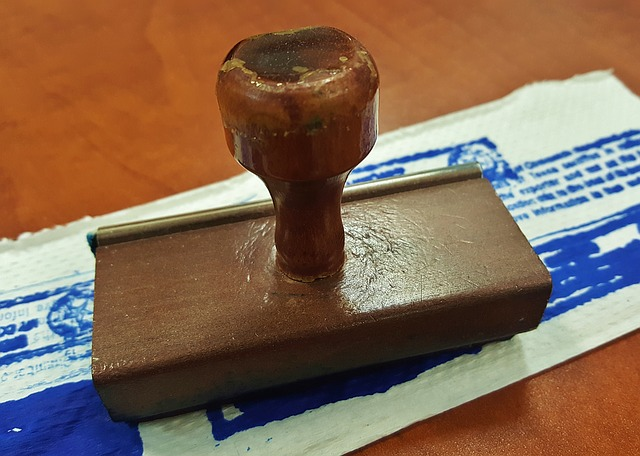
\includegraphics[width=0.5\textwidth]{../img/stamp}

\columnbreak

\pause

\begin{itemize}
\item En stämpel kan \Alert{tillverkas} -- motsvarar \Emph{deklaration} av klassen.
 \item Det händer inget förrän man \Alert{stämplar} -- motsvarar \Emph{instansiering}.
\item Då skapas \Alert{avbildningar} av stämpeln -- motsvarar \Emph{allokering av ett objekt} som är en \Emph{instans} av klassen.
\item Allokering kallas också \Emph{konstruktion} och funktionen/koden som gör själva allokeringen kallas \Emph{konstruktor}.
\end{itemize}

\end{multicols}
\end{Slide}


\begin{Slide}{Vad är en klass?}
\begin{itemize}
\item En klass är en mall \Eng{template} för att skapa objekt.
\item Objekt kan skapas med \code{new Klassnamn}, vilket kallas \Emph{instansiering}. 
\item I Scala 3 är \code{new} valfritt, det räcker med \code{Klassnamn()}. 
\item Ett objekt som skapats med en klassen \code{Klassnamn} som mall kallas för en \Emph{instans} av klassen \code{Klassnamn}.
\item En klass innehåller \Emph{medlemmar} \Eng{members}, som bl.a. kan vara:
  \begin{itemize}
  \item \Emph{attribut}, kallas även fält \Eng{field}: \code{val}, \code{lazy val}, \code{var}
  \item \Emph{metoder}, kallas även operationer: \code{def}
  \end{itemize}
\item Varje instans har sin uppsättning värden på attributen
vilka tillsammans utgör instansens \Emph{tillstånd}.
\end{itemize}

\end{Slide}
  


% \begin{Slide}[t]{Klass och instans}
% \vspace{-0.65em}
% \begin{REPLnonum}
% scala> class C { var attr = 42 }
%
% scala> val objRef1 = new C
% \end{REPLnonum}
% \vspace{3.7em}
% \begin{tikzpicture}[font=\SlideFontSmall\sffamily]
% \matrix [matrix of nodes, row sep=0, column 2/.style={nodes={rectangle,draw,minimum width=0.8cm}}] (mat)
% {
% \texttt{objRef1}   &  \makebox(10,10){ }\\
% };
%
% \node[cloud, cloud puffs=15.0, cloud ignores aspect, minimum width=2cm, minimum height=2cm,
%  align=center, draw] (instance1) at (3.8cm, 0.0cm) {
%  \begin{tabular}{r l}
%  \texttt{attr} & \fbox{42} \\
%  \end{tabular}
%  };
%
%
% \filldraw[black] ($ (mat-1-2) + (0.0cm,0.0cm) $) circle (3pt) node[] (ref1)  {};
% \draw [arrow, line width=0.7mm] (ref1) -- (instance1);
% \end{tikzpicture}
% \end{Slide}
%
%
%
% \begin{Slide}[t]{Klass och instans}
% \vspace{-0.5em}
% \begin{REPLnonum}
% scala> class C { var attr = 42 }
%
% scala> val objRef1 = new C
%
% scala> val objRef2 = new C
% \end{REPLnonum}
% \vspace{2em}
% \begin{tikzpicture}[font=\SlideFontSmall\sffamily]
% \matrix [matrix of nodes, row sep=0, column 2/.style={nodes={rectangle,draw,minimum width=0.8cm}}] (mat)
% {
% \texttt{objRef1}   &  \makebox(10,10){ }\\
% \texttt{objRef2}   &  \makebox(10,10){ }\\
% };
%
% \node[cloud, cloud puffs=15.0, cloud ignores aspect, minimum width=2cm, minimum height=2cm,
%  align=center, draw] (instance1) at (3.8cm, 0.35cm) {
%  \begin{tabular}{r l}
%  \texttt{attr} & \fbox{42} \\
%  \end{tabular}
%  };
%
% \node[cloud, cloud puffs=15.0, cloud ignores aspect, minimum width=2cm, minimum height=2cm,
%  align=center, draw] (instance2) at (5.8cm, -1.5cm) {
%  \begin{tabular}{r l}
%  \texttt{attr} & \fbox{42} \\
%  \end{tabular}
%  };
%
% \filldraw[black] ($ (mat-1-2) + (0.0cm,0.0cm) $) circle (3pt) node[] (ref1)  {};
% \draw [arrow, line width=0.7mm] (ref1) -- (instance1);
%
% \filldraw[black] ($ (mat-2-2) + (0.0cm,0.0cm) $) circle (3pt) node[] (ref2)  {};
% \draw [arrow, line width=0.7mm] (ref2) -- (instance2);
% \end{tikzpicture}
% \end{Slide}
%
%
%
% \begin{Slide}[t]{Klass och instans}
% \vspace{-0.5em}
% \begin{REPLnonum}
% scala> class C { var attr = 42 }
%
% scala> val objRef1 = new C
%
% scala> val objRef2 = new C
%
% scala> objRef2.attr = 43
% \end{REPLnonum}
% \begin{tikzpicture}[font=\SlideFontSmall\sffamily]
% \matrix [matrix of nodes, row sep=0, column 2/.style={nodes={rectangle,draw,minimum width=0.8cm}}] (mat)
% {
% \texttt{objRef1}   &  \makebox(10,10){ }\\
% \texttt{objRef2}   &  \makebox(10,10){ }\\
% };
%
% \node[cloud, cloud puffs=15.0, cloud ignores aspect, minimum width=2cm, minimum height=2cm,
%  align=center, draw] (instance1) at (3.8cm, 0.35cm) {
%  \begin{tabular}{r l}
%  \texttt{attr} & \fbox{42} \\
%  \end{tabular}
%  };
%
% \node[cloud, cloud puffs=15.0, cloud ignores aspect, minimum width=2cm, minimum height=2cm,
%  align=center, draw] (instance2) at (5.8cm, -1.5cm) {
%  \begin{tabular}{r l}
%  \texttt{attr} & \fbox{43} \\
%  \end{tabular}
%  };
%
%
% \filldraw[black] ($ (mat-1-2) + (0.0cm,0.0cm) $) circle (3pt) node[] (ref1)  {};
% \draw [arrow, line width=0.7mm] (ref1) -- (instance1);
%
% \filldraw[black] ($ (mat-2-2) + (0.0cm,0.0cm) $) circle (3pt) node[] (ref2)  {};
% \draw [arrow, line width=0.7mm] (ref2) -- (instance2);
% \end{tikzpicture}
% \end{Slide}



\begin{Slide}{Singelobjekt jämfört med klass}\SlideFontSmall
Vi har tidigare deklarerat \Emph{singelobjekt} som bara finns i \Alert{en} enda upplaga:
\begin{REPLnonum}
scala> object Björn { var ålder = 53; val längd = 178 }
\end{REPLnonum}

Med en \Emph{klass} kan man skapa \Alert{godtyckligt många} \Emph{instanser av klassen} med hjälp av nyckelordet \code{new} följt av klassens namn:

\begin{REPLnonum}
scala> class Person { var ålder = 0; var längd = 0 }

scala> val björn = new Person   // allokera plats i minnet
björn: Person = Person@7ae75ba6  // unikt id för instansen
\end{REPLnonum}
\begin{tikzpicture}[font=\small\sffamily]
\matrix [matrix of nodes, row sep=0, column 2/.style={nodes={rectangle,draw,minimum width=0.8cm}}] (mat)
{
\texttt{björn}   &  \makebox(10,10){ }\\
};
\node[cloud, cloud puffs=12.0, cloud ignores aspect, minimum width=2cm, minimum height=3.8cm,
 align=center, scale=0.8, draw] (x) at (3.8cm, -1.0cm) {
 \begin{tabular}{r l}
 \multicolumn{2}{c}{\ttfamily\itshape Person@7ae75ba6}\\ \\
 \texttt{ålder} & \fbox{~0~} \\
 \texttt{längd} & \fbox{~0~}\\
 \end{tabular}
 };
\filldraw[black] (0.6cm,0.0cm) circle (3pt) node[] (ref) {};
\draw [arrow, line width=0.7mm] (ref) -- (x);
\end{tikzpicture}
\end{Slide}


\begin{Slide}{Förändring av objektets tillstånd}
\begin{REPLnonum}
scala> björn.ålder = 53

scala> björn.längd = 178
björn: Person = Person@7ae75ba6
\end{REPLnonum}

\begin{tikzpicture}[font=\large\sffamily]
\matrix [matrix of nodes, row sep=0, column 2/.style={nodes={rectangle,draw,minimum width=0.8cm}}] (mat)
{
\texttt{björn}   &  \makebox(10,10){ }\\
};
\node[cloud, cloud puffs=13.0, cloud ignores aspect, minimum width=2cm, minimum height=3.8cm,
 align=center, draw] (x) at (5.8cm, -1.2cm) {
 \begin{tabular}{r l}
 \multicolumn{2}{c}{\ttfamily\itshape Person@7ae75ba6}\\ \\
 \texttt{ålder} & \fbox{~53~} \\
 \texttt{längd} & \fbox{~178~}\\
 \end{tabular}
 };
\filldraw[black] (0.75cm,0.0cm) circle (3pt) node[] (ref) {};
\draw [arrow, line width=0.7mm] (ref) -- (x);
\end{tikzpicture}
%{\SlideFontTiny{\ttfamily\itshape Person@7ae75ba6} är en unik idenfierare för instansen, så att JVM hittar den i heapen.}
\end{Slide}


\begin{Slide}{Bättre att initialisera med hjälp av klassparametrar}
\begin{REPLnonum}
scala> class Person(var ålder: Int, var längd: Int)

scala> val sandra = new Person(42, 166)
sandra: Person = Person@7878bbdb
\end{REPLnonum}

\begin{tikzpicture}[font=\large\sffamily]
\matrix [matrix of nodes, row sep=0, column 2/.style={nodes={rectangle,draw,minimum width=0.8cm}}] (mat)
{
\texttt{sandra}   &  \makebox(10,10){ }\\
};
\node[cloud, cloud puffs=13.0, cloud ignores aspect, minimum width=2cm, minimum height=3.8cm,
 align=center, draw] (x) at (5.8cm, -1.2cm) {
 \begin{tabular}{r l}
 \multicolumn{2}{c}{\ttfamily\itshape Person@7878bbdb}\\ \\
 \texttt{ålder} & \fbox{~42~} \\
 \texttt{längd} & \fbox{~166~}\\
 \end{tabular}
 };
\filldraw[black] (0.75cm,0.0cm) circle (3pt) node[] (ref) {};
\draw [arrow, line width=0.7mm] (ref) -- (x);
\end{tikzpicture}
%{\SlideFontTiny{\ttfamily\itshape Person@7ae75ba6} är en unik idenfierare för instansen, så att JVM hittar den i heapen.}
\end{Slide}


\begin{Slide}{Klassdeklarationer och instansiering}\SlideFontSmall
\setlength{\leftmargini}{0pt}
\begin{itemize}
\item Syntax för deklaration av klass: \\ \vspace{0.5em}{\SlideFontSize{13}{16}\code|class Klassnamn(parametrar){ medlemmar }|}\vspace{0.5em}
\item Exempel: \Emph{deklaration}
\begin{Code}
class Klassnamn(val attribut1: Int, attribut2: String){
  val attribut3: Double = 42.0              //publikt oföränderligt attribut
  private var attribut4: Boolean = false    //privat medlem syns inte utåt
  def metod(parameter: Int) = parameter + 1 //funktion i klass kallas metod
  lazy val attr5 = Vector.fill(100000)(42.0)     //fördröjd initialisering
}
\end{Code}

\item Parametrar initialiseras med de argument som ges vid \code{new}.
\item Exempel: \Emph{instansiering} med argument för initialisering av klassparametrar
\begin{Code}
val instansReferens = new Klassnamn(42, "hej")  // new är valfritt här 
\end{Code}

\item Parametrar som inte föregås av modifierare (t.ex. private val, val, var) blir \Emph{attribut} som är \code{ private[this] val } och bara är synliga i \Alert{denna} instans.
\item Attribut i klasskroppen är \Emph{publika} (alltså synliga utåt) om inte \code{private} anges.
\end{itemize}
\end{Slide}




\begin{Slide}{Övning: en klass som representerar en person}
\begin{enumerate}
  \item Deklarera en klass \code{Person} med dessa publika attribut:
  \begin{itemize}
    \item oföränderligt förnamn
    \item oföränderligt efternamn
    \item förändringsbar ålder med defaultargument \code{0}
  \end{itemize}
  \item lägg till en metod i klasskroppen med explicit returtyp som ger en 2-tupel med förnamn och efternamn
  \item skriv en deklaration som deklarerar en variabel \code{p} som initialiseras med värdet av ett uttryck som instansierar klassen \code{Person} med ditt namn och din ålder som nyfödd.
  \item skriv en sats som skriver ut ditt förnamn genom att referera attribut med punktnotation
  \item skriv en tilldelningssats som ändrar tillståndet för den instans som referensen \code{p} refererar till så att åldersattributets värde blir din nuvarande ålder
\end{enumerate}
\end{Slide}



\begin{Slide}{Lösning: klassen Person}
\begin{Code}[basicstyle=\SlideFontSize{6.9}{9}\ttfamily]
class Person(val givenName: String, val familyName: String, var age: Int = 0){
  def name: (String, String) = (givenName, familyName)
}
\end{Code}
\begin{REPLnonum}[basicstyle=\SlideFontSize{7}{9}\ttfamily\color{white}]
val p = Person("Björn", "Regnell")
println(p.name._1)
p.age = 50
\end{REPLnonum}
\end{Slide}


\begin{Slide}{Instansprivata klassparametrar}\SlideFontSmall
\setlength{\leftmargini}{0pt}

\begin{itemize}
\item Parametrar som inte föregås av modifierare (t.ex. private val, val, var) blir \Emph{attribut} som är \code{ private[this] val } och bara är synliga i \Alert{denna} instans.
\item Exempel på konsekvensen av \code{private[this]}:
\begin{REPL}[basicstyle=\SlideFontSize{6.7}{9}\ttfamily\color{white}]
scala> class C(a: Int){ def add(other: C): Int = a + other.a }
error: value a is not a member of C

// betyder samma sak som:

scala> class C(private[this] val a: Int){ def add(other: C): Int = a + other.a }
error: value a is not a member of C
\end{REPL}
\item Men detta fungerar fint:
\begin{REPL}
scala> class D(val a: Int){ def add(other: D): Int = a + other.a }

scala> D(42).add(D(43))
res0: Int = 85
\end{REPL}
...eftersom modifieraren \code{val} framför klassparameter ger publik synlighet.
\item Vad händer om du skriver \code{private val} framför klassparametern \code{a} ovan?
\end{itemize}
\end{Slide}


\begin{Slide}{\texttt{private} jämfört med \texttt{private[this]}}\SlideFontSmall
\code{private[this]} är \Alert{ännu} mer privat än \code{private}
\begin{Code}
class Hemlis(private val hemlis: Int) {
  def ärSammaSom(annan: Hemlis) = hemlis == annan.hemlis   // Funkar!
}

class Hemligare(private[this] val hemlis: Int) {
  def ärSammaSom(annan: Hemligare) = hemlis == annan.hemlis //KOMPILERINGSFEL
}
\end{Code}
\pause Vad händer om man inte skriver ens \code{val}? \pause Olika för klass och s.k. case-klass:
\begin{Code}
class Hemligare(hemlis: Int) { // motsvarar private[this] val
  def ärSammaSom(annan: Hemligare) = hemlis == annan.hemlis //KOMPILERINGSFEL
}

case class InteHemlig(seMenInteRöra: Int) { // blir automatiskt val
  def ärSammaSom(annan: InteHemlig): Boolean =
    seMenInteRöra == annan.seMenInteRöra
}

\end{Code}
{\SlideFontTiny Vi ska lära mer om det godis man får på köpet med \code{case}-klasser om ett litet tag.}
\end{Slide}



%%%%%%%%%%%% ÄR EXEMPEL KOMPLEXA TAL ÄR FÖR SVÅR MATEMATIK för lp1???? %%%%%%%%%
%% Nej komplexa tal som vektor med polära koordinater ingår i matte 4 som är krav för LTH: %%%


\begin{Slide}{Övning: Klassen Complex i Scala}\SlideFontSmall
Implementera klassen \code{Complex} nedan som representerar komplexa tal:
\begin{Code}
  class Complex(val re: Double, val im: Double):
    def r  = ???  // absolutbeloppet
    def fi = ???  // vinkeln i radianer
    def +(other: Complex): Complex = ???  // resultatet av addition
    var imSymbol = 'i'  // symbol för imaginärdel, används i toString
    override def toString = ???  // en strängrepresentation av talet
\end{Code}

\begin{minipage}{0.3\textwidth}
  Exempel: \\$z = 3 + 4i$
\end{minipage}
\begin{minipage}{0.5\textwidth}
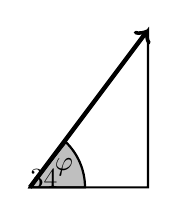
\begin{tikzpicture}[thick]
\coordinate (O) at (0,0);
\coordinate (A) at (1.5,0);
\coordinate (B) at (1.5,2.0);

%\tkzMarkAngle[fill=orange,size=0.5cm, opacity=.4](A,O,B) 
%\tkzLabelAngle[pos=0.8](A,O,B){\texttt{$\varphi$}}
 %%% AAAARGH ovan slutade funka så gjorde nedan HACK i stället
\draw[fill=lightgray, thick] (0,0) -- (0:0.7cm) arc (0:46:0.8cm) node at (30:0.5cm) {$\varphi$} -- cycle;
%\draw[fill=lightgray, thick] (0,0) -- (0:0.7cm) arc (0:45:0.8cm) node at (30:0.5cm) {$\varphi$} -- cycle;
%https://tex.stackexchange.com/questions/96459/automatically-draw-and-labels-angles-of-a-triangle-in-tikz

\draw (O)--(A)--(B)--cycle;
\draw [->, ultra thick] (O)--(B);

\tkzLabelSegment[below=5pt](O,A){\textit{real-delen} är $3$}
\tkzLabelSegment[above left=5pt](O,B){\textit{r}}
\tkzLabelSegment[right=5pt](A,B){\textit{imaginär-delen} är $4$}


\end{tikzpicture}
\end{minipage}

\end{Slide}


\begin{Slide}{Exempel: Klassen Complex i Scala}\SlideFontSmall
\scalainputlisting[basicstyle=\ttfamily\SlideFontSize{7}{9}]{../compendium/examples/complex1.scala}
%Klassparametrarna är parametrar till den s.k. \Emph{primärkonstruktorn}.
\begin{REPL}
scala> val z = new Complex(3, 4)  // konstruktion av instans av Complex
z: Complex = 3.0 + 4.0i

scala> val polärForm = (c1.r, c1.fi)
polärForm: (Double, Double) = (5.0,0.6435011087932844)

scala> val z2 = new Complex(1, 2)
z2: Complex = 1.0 + 2.0i

scala> z1 + z2
res0: Complex = 4.0 + 6.0i
\end{REPL}
\end{Slide}



\begin{Slide}{Exempel: Principen om enhetlig access}\SlideFontSmall
\scalainputlisting[basicstyle=\ttfamily\SlideFontSize{7}{9}]{../compendium/examples/complex2.scala}
\pause
\begin{itemize}
\item Efter som attributen \code{re} och \code{im} är oföränderliga, kan vi lika gärna ändra i klass-implementationen och göra om metoderna \code{r} och \code{fi} till \code{val}-variabler utan att klientkoden påverkas.

\item Då anropas \code{math.hypot} och \code{math.atan2} bara en gång vid initialisering (och inte varje gång som med \code{def}).

\item Vi skulle även kunna använda \code{lazy val} och då bara räkna ut \code{r} och \code{fi} om och när de verkligen refereras av klientkoden, annars inte.

\item Eftersom klientkoden inte ser skillnad på metoder och variabler, kallas detta \Emph{principen om enhetlig access}. (Många andra språk har \Alert{inte} denna möjlighet, tex Java där metoder \emph{måste} ha parenteser.)
\end{itemize}
\end{Slide}



\Subsection{Olika sätt att skapa instanser}

\begin{Slide}{Instansiering med direkt användning av \texttt{new}}

Instansiering genom \Emph{direkt användning} av \code{new}\\
{\SlideFontSmall (här första varianten av Complex med \code{r} och \code{fi} som metoder)}
\begin{REPLnonum}
scala> val c1 = new Complex(3, 4)
\end{REPLnonum}
\begin{tikzpicture}[font=\SlideFontSmall\sffamily]
\matrix [matrix of nodes, row sep=0, column 2/.style={nodes={rectangle,draw,minimum width=0.8cm}}] (mat)
{
\texttt{c1}   &  \makebox(10,10){ }\\
};

\node[cloud, cloud puffs=15.0, cloud ignores aspect, minimum width=2cm, minimum height=3.8cm,
 align=center, draw] (instance1) at (5.8cm, -1.5cm) {
 \begin{tabular}{r l l}
 \texttt{re:} & \texttt{Double} & \fbox{3.0} \\
 \texttt{im:} & \texttt{Double} & \fbox{4.0}\\
 \texttt{imSymbol:} & \texttt{Char} & \fbox{i}\\
 \end{tabular}
 };

\filldraw[black] ($ (mat-1-2) + (0.0cm,0.0cm) $) circle (3pt) node[] (ref1)  {};

\draw [arrow, line width=0.7mm] (ref1) -- (instance1);
\end{tikzpicture}
\pause
Ofta vill man göra \Alert{indirekt} instansiering så att vi senare har friheten att ändra hur instansiering sker.
\end{Slide}



\begin{Slide}{Indirekt instansiering med fabriksmetoder}\SlideFontSmall
En \Emph{fabriksmetod} är en metod som används för att instansiera objekt.
\begin{Code}[basicstyle=\SlideFontSize{8}{12}\ttfamily\selectfont]
object MyFactory {
  def createComplex(re: Double, im: Double) = new Complex(re, im)
  def createReal(re: Double)                = new Complex(re, 0)
  def createImaginary(im: Double)           = new Complex(0, im)
}
\end{Code}
\pause
Instansiera \Alert{inte direkt}, utan \Emph{indirekt} genom användning av \Emph{fabriksmetoder}:
\begin{REPL}
scala> import MyFactory._

scala> createComplex(3, 4)
res0: Complex = 3.0 + 4.0i

scala> createReal(42)
res1: Complex = 42.0 + 0.0i

scala> createImaginary(-1)
res2: Complex = 0.0 + -1.0i
\end{REPL}
\end{Slide}



\begin{Slide}{Hur förhindra direkt instansiering?}
Om vi vill \Emph{förhindra direkt instansiering} kan vi göra primärkonstruktorn \Alert{privat}:
\scalainputlisting[basicstyle=\ttfamily\SlideFontSize{7}{9}]{../compendium/examples/complex3.scala}
MEN... då går det ju \Alert{inte} längre att instansiera något alls!  \code{   :(}
\begin{REPLnonum}
scala> new Complex(3,4)
error:
 constructor Complex in class Complex cannot be accessed
\end{REPLnonum}
\end{Slide}



\begin{Slide}{Kompanjonsobjekt med indirekt instansiering}\SlideFontSmall
\setlength{\leftmargini}{0pt}
\begin{itemize}
\item Ett \Emph{kompanjonsobjekt} \Eng{companion object} är ett singelobjekt som ligger i \Alert{samma kodfil} som en klass, och som har \Alert{samma namn} som klassen.

\item Medlemmar i ett kompanjonsobjekt \Alert{får accessa privata} medlemmar i kompanjonsklassen (och vice versa) och kompanjonsobjektet får därför accessa privat konstruktor och kan göra \code{new}.
\scalainputlisting[basicstyle=\ttfamily\SlideFontSize{7}{9}]{../compendium/examples/complex4.scala}

\item Fabriksmetoder i kompanjonsobjektet ovan och privat konstruktor gör att vi \Alert{enbart} tillåter \Emph{indirekt instansiering}.
\end{itemize}
\end{Slide}

\begin{Slide}{Användning av kompanjonsobjekt med fabriksmetoder}
Nu kan vi \Alert{bara} instansiera \Emph{indirekt}!  \code{   :)}
\begin{REPLnonum}
scala> Complex.real(42.0)
res0: Complex = 42.0 + 0.0i

scala> Complex.imag(-1)
res1: Complex = 0.0 + -1.0i

scala> Complex.apply(3,4)
res2: Complex = 3.0 + 4.0i

scala> Complex(3,4)
res3: Complex = 3.0 + 4.0i

scala> new Complex(3, 4)
error:
     constructor Complex in class Complex cannot be accessed
\end{REPLnonum}
\end{Slide}


\begin{Slide}{Alternativa direktinstansieringar med default-argument}\SlideFontSmall
Med \Emph{default-argument} kan vi erbjuda \Emph{alternativa} sätt att direktinstansiera.
\scalainputlisting[basicstyle=\ttfamily\SlideFontSize{7}{9}]{../compendium/examples/complex5.scala}
\begin{REPL}
scala> new Complex()
res0: Complex = 0.0 + 0.0i

scala> new Complex(re = 42)  //anrop med namngivet argument
res1: Complex = 42.0 + 0.0i

scala> new Complex(im = -1)
res2: Complex = 0.0 + -1.0i

scala> new Complex(1)
res3: Complex = 1.0 + 0.0i
\end{REPL}
\end{Slide} 

\begin{Slide}{Alternativa sätt att instansiera med fabriksmetod}
Vi kan också erbjuda \Emph{alternativa} sätt att instansiera \Emph{indirekt} med fabriksmetoden \code{apply} i ett kompanjonsobjekt genom default-argument:
\scalainputlisting[basicstyle=\ttfamily\SlideFontSize{7}{9}]{../compendium/examples/complex6.scala}

\end{Slide}

\begin{Slide}{Medlemmar som bara behövs i en enda upplaga}
Attributet \code{imSymbol} passar bättre att ha i \Emph{kompanjonsobjektet}, eftersom det räcker att ha \Alert{en enda upplaga}, som kan vara gemensam för alla objekt:
\scalainputlisting[basicstyle=\ttfamily\SlideFontSize{7}{9}]{../compendium/examples/complex7.scala}

\end{Slide}



\begin{Slide}{Medlemmar i singelobjekt är statiskt allokerade}\SlideFontTiny

Minnesplatsen för \Emph{attribut i singelobjekt} allokeras automatiskt en gång för alla, och kallas därför \Emph{statiskt} allokerad. Singelobjektets namn \code{Complex} utgör en statisk referens till den enda instansen och är av typen \texttt{Complex.type}.

\begin{tikzpicture}[font=\SlideFontSmall\sffamily]
\matrix [matrix of nodes, row sep=0, column 2/.style={nodes={rectangle,draw,minimum width=0.8cm}}] (mat)
{
\texttt{Complex}   &  \makebox(10,10){ }\\
};

\node[cloud, cloud puffs=15.0, cloud ignores aspect, minimum width=1cm, minimum height=2cm,
 align=center, draw] (instance1) at (5.8cm, 0.0cm) {
 \begin{tabular}{r l l}
 \texttt{imSymbol:} & \texttt{Char} & \fbox{i}\\
 \end{tabular}
 };

\filldraw[black] ($ (mat-1-2) + (0.0cm,0.0cm) $) circle (3pt) node[] (ref1)  {};

\draw [arrow, line width=0.7mm] (ref1) -- (instance1);
\end{tikzpicture}

Nu bereder vi inte plats för \code{imSymbol} i varenda \Emph{dynamiskt} allokerade instans:
\begin{REPLnonum}
scala> val c1 = Complex(3, 4)
\end{REPLnonum}

\begin{tikzpicture}[font=\SlideFontSmall\sffamily]
\matrix [matrix of nodes, row sep=0, column 2/.style={nodes={rectangle,draw,minimum width=0.8cm}}] (mat)
{
\texttt{c1}   &  \makebox(10,10){ }\\
};

\node[cloud, cloud puffs=15.0, cloud ignores aspect, minimum width=2cm, minimum height=2cm,
 align=center, draw] (instance1) at (5.8cm, -0.0cm) {
 \begin{tabular}{r l l}
 \texttt{re:} & \texttt{Double} & \fbox{3.0} \\
 \texttt{im:} & \texttt{Double} & \fbox{4.0}\\
 \end{tabular}
 };

\filldraw[black] ($ (mat-1-2) + (0.0cm,0.0cm) $) circle (3pt) node[] (ref1)  {};

\draw [arrow, line width=0.7mm] (ref1) -- (instance1);
\end{tikzpicture}


\end{Slide}




\begin{Slide}{Attribut i kompanjonsobjekt användas för sådant som är gemensamt för alla instanser}

Om vi ändrar på statiska \code{imSymbol} så ändras \code{toString} för \Alert{alla} dynamiskt allokerade instanser.
\begin{REPLnonum}
scala> val c1 = Complex(3, 4)
c1: Complex = 3.0 + 4.0i

scala> Complex.imSymbol = 'j'
Complex.imSymbol: Char = j

scala> val c2 = Complex(5, 6)
c2: Complex = 5.0 + 6.0j

scala> c1
res0: Complex = 3.0 + 4.0j
\end{REPLnonum}
\end{Slide}


\Subsection{Case-klasser och fördelen med oföränderlighet}

\ifkompendium\else
\begin{frame}[plain]
  
\includegraphics[width=1.0\textwidth]{../img/mutant.png}
\end{frame}
\fi

\begin{Slide}{Övning: en läskig mutant}\SlideFontSmall
\begin{enumerate}
\item Skapa en klass med namnet \code{Mutant} som har ett förändringsbart attribut som klassparameter med namnet \code{i} av typen \code{Int} med default-argumentet \code{5}.
\vspace{0.5em}

\item \begin{minipage}{0.5\textwidth}
Deklarera två \code{val}-variabler som kallas \code{fem1} och \code{fem2} och som båda refererar till \Alert{samma} \code{Mutant}-instans.
\end{minipage}
\hfill\begin{minipage}{0.32\textwidth}
\hfill
\includegraphics[width=3.4cm]{../img/mutant.png}

En \code{Mutant}-instans där \code{i} kanske är fem.
\vspace{1em}
\end{minipage}

\item Skriv kod som ändrar tillstånd via den ena mutantreferensen.

\item Syns ändringen via den andra mutantreferensen?
\end{enumerate}
\end{Slide}




\begin{Slide}{Case-klasser}
Case-klasser är ett smidigt sätt att skapa \Emph{oföränderliga} datastrukturer. Med nyckelordet \code{case} framför \code{class} får du mycket ''godis på köpet'':

\begin{itemize}
\item Klassparametrar blir automatiskt publika oföränderliga attribut\footnote{alltså \Alert{inte} \texttt{private[this] val } som i vanliga klasser.} och du slipper alltså skriva \code{val}
\item Du får en automatisk \Emph{toString} med klassens namn och värdet av alla \code{val}-attribut som ges av klassparametrarna och du slipper alltså skriva en egen toString
\item Du får ett automatiskt kompanjonsobjekt med en fabriksmetod \code{apply} för indirekt instansiering där alla klassparametrarnas \code{val}-attribut initialiseras.
\pause
\item ... och mer därtill men mer om det senare...
\end{itemize}
\end{Slide}




\begin{Slide}{Exempel: oföränderliga case-klassen \code{Point}}

\begin{Code}[basicstyle=\SlideFontSize{10}{12}\ttfamily]
case class Point(x: Double, y: Double)
\end{Code}

\begin{REPLnonum}
scala> val p1 = Point(3, 4)
p1: Point = Point(3.0,4.0)

scala> val p2 = p1
p2: Point = Point(3.0,4.0)

scala> p1.x = 42
error: reassignment to val
\end{REPLnonum}
Vi kan utan risk dela med oss av en referens till en oföränderlig klass -- ingen kan ändra dess innehåll. (Jämför läskiga mutanten i tidigare exempel.)

\end{Slide}






\Subsection{Konstruktor}



\begin{Slide}{Vad är en konstruktor?}
\begin{itemize}
\item En \Emph{konstruktor} är den maskinkod som exekveras när klasser instansieras med \code{new}.

\item Konstruktorn skapar ett nytt objekt i minnet vid varje anrop.

\item I Scala \Alert{genererar kompilatorn} en \Emph{primärkonstruktor} åt dig med maskinkod som initialiserar alla attribut baserat på klassparametrarna som du deklarerat.

\pause

%\item I Java och många andra språk får man \Alert{explicit} skriva kod för konstruktorer med speciell syntax och göra alla initialiseringar av attribut själv, och det behövs många olika konstruktorer för att motsvara defaultargument.

\item I Scala \Emph{kan} man också skriva egna alternativa s.k. \Emph{hjälpkonstruktorer}, men det är \Alert{ovanligt}, eftersom man har möjligheten med fabriksmetoder i kompanjonsobjekt och default-argument.
\end{itemize}
\end{Slide}


\begin{Slide}{Hjälpkonstruktorer i Scala (ovanliga)}%\SlideFontSmall
Fördjupning för kännedom:
\begin{itemize}
\item I Scala kan man skapa ett alternativ till primärkonstruktorn, en så kallad \Emph{hjälpkonstruktor} \Eng{auxilliary constructor} genom att deklarera en metod med det speciella namnet \code{this}.


\item Hjälpkonstruktorer \Alert{måste} börja med att anropa en \Alert{annan} konstruktor som står \Alert{före} i koden, till exempel primärkonstruktorn.
\end{itemize}

\begin{Code}
class Point(val x: Int, val y: Int, val z: Int): // primärkonstruktor
  def this(x: Int, y: Int) = this(x, y, 0) // anropa primärkonstruktorn
  def this(x: Int) = this(x, 0) // anropa hjälpkonstruktor
\end{Code}

%{\SlideFontSmall Överlagrade hjälpkonstruktorer i Scala liknar användning av konstruktorer i Java, där man inte har default-argument och apply i kompanjonsobj. etc.}

\end{Slide}

\begin{Slide}{Användning av hjälpkonstruktor}
\begin{REPL}
scala> val p1 = Point(1)
p1: Point = Point@21312342

scala> val p2 = Point(1, 2)
p2: Point = Point@43254325

scala> val p3 = Point(1, 2, 3)
p3: Point = Point@346654
\end{REPL}
\pause
Men man gör \Alert{mycket oftare} så här i Scala:
\begin{Code}[basicstyle=\ttfamily\SlideFontSize{8.5}{12}]
case class Point(x: Int, y: Int = 0, z: Int = 0)
\end{Code}
Använd alltså defaultargument hellre än hjälpkonstruktor.\\
(Eller överlagrad fabriksmetod i kompanjonsobjekt.)
\end{Slide}



% \begin{Slide}{Vad gör skräpsamlaren?}\SlideFontSmall
% \begin{itemize}
% \item Scala och Java är båda programmeringsspråk som förutsätter en körmiljö med \Alert{automatisk}  \Emph{skräpsamling} \Eng{garbage collection}.
%
% \item \Emph{Skräpsamlaren} \Eng{the garbage collector} är ett program som automatiskt körs i bakgrunden då och då och \Emph{städar minnet} genom att frigöra den plats som upptas av \Alert{objekt som inte längre används}.
%
% \item JVM:en bestämmer själv när skräpsamlaren ska jobba och programmeraren har ingen kontroll över detta.
%
% \item Den stora \Emph{fördelen} med automatisk skärpsamling är att man slipper bry sig om det svåra och felbenägna arbetet att \Alert{avallokera} minne.
%
% \item \Alert{Nackdelen} är att man inte kan styra exakt hur och när skräpsamlingen ska ske och man kan därmed inte bestämma när processorn ska belastas med minneshanteringen. Detta är normalt inget problem, utom i vissa tidskritiska realtidssystem med hårda minnesbegränsningar och svarstidskrav.
%
% \item I språk utan automatisk skräpsamling, t.ex. C++, måste man ta hand om destruktion av objekt och skriva egna s.k. \Emph{destruktorer}.
% \end{itemize}
% \end{Slide}


\Subsection{Referens saknas: \texttt{null}}

\begin{Slide}{Referens saknas: \texttt{null}}
\begin{itemize}
\item I Java och många andra språk använder man ofta literalen \code{null} för att representera att ett \Alert{värde saknas}.

\item En referens som är \code{null} refererar inte till någon instans.

\item Om du försöker referera till instansmedlemmar med punktnotation genom en referens som är \code{null} kastas ett \Alert{undantag} \code{NullPointerException}.

\item Oförsiktig användning av \code{null} är en vanlig källa till \Alert{buggar}, som kan vara svåra att hitta och fixa.

\end{itemize}
\end{Slide}


\begin{Slide}{Exempel: \texttt{null}}
\begin{REPL}
scala> class Gurka(val vikt: Int)

scala> var g: Gurka = null        // ingen instans allokerad än
val g: Gurka = null

scala> g.vikt
java.lang.NullPointerException

scala> g = Gurka(42)          // instansen allokeras
val g: Gurka = Gurka@1ec7d8b3

scala> g.vikt
val res0: Int = 42

scala> g = null         // instansen kommer att destrueras av skräpsamlaren
\end{REPL}

\begin{itemize} \SlideFontSmall
\item Scala har \code{null} av kompabilitetsskäl, men det är brukligt att \Alert{endast} använda \code{null} om man anropar Java-kod.

\item Scala erbjuder smidiga \code{Option}, \code{Some} och \code{None} för säker hantering av saknade värden; mer om detta kommande vecka.



\end{itemize}
\end{Slide}


\Subsection{Referensen \texttt{this}}
\begin{Slide}{Referensen \texttt{this}}\SlideFontSmall
\begin{itemize}
\item Nyckelordet \code{this} ger en referens till den aktuella instansen.
\begin{REPLnonum}
scala> class Gurka(var vikt: Int){def jagSjälv = this}

scala> val g = Gurka(42)
val g: Gurka = Gurka@5ae9a829

scala> g.jagSjälv
val res0: Gurka = Gurka@5ae9a829

scala> g.jagSjälv.vikt
val res1: Int = 42

scala> g.jagSjälv.jagSjälv.vikt
val res2: Int = 42
\end{REPLnonum}
\item Referensen \code{this} används ofta för att komma runt ''namnkrockar'' där variabler med samma namn gör så att den ena variabeln inte syns.
\end{itemize}
\end{Slide}



\Subsection{Getters och setters}

\begin{Slide}{Getters och setters}\SlideFontSmall
\begin{itemize}
\item I många språk (t.ex. Java, Python) finns inget motsvarande nyckelord \code{val} som garanterar oföränderliga attributreferenser.
\footnote{Java har visserligen \jcode{final} men det är annorlunda som vi ska se senare.}

\item Därför gör man i dessa språk nästan alltid alla attribut \Alert{privata} för att förhindra att de ändras på ett okontrollerat sätt.

% \item Många språk följer \Alert{inte} principen om enhetlig access: åtkomst av metoder och variabler sker med olika syntax.

\item Därför är det normalt att införa metoder som kallas \Emph{getters} och \Emph{setters}, som används för att \Alert{indirekt} läsa och uppdatera \Emph{attribut}.

\item Dessa metoder känns i många språk igen genom konventionen att de heter något som börjar med \Emph{get} respektive \Emph{set}. (Men \Alert{ej} vanligt i Scala.)

\item Med \Emph{indirekt access} av attribut kan man åstadkomma \Emph{flexibilitet}, så att implementationen kan ändras utan att ändra i klientkoden:
\begin{itemize}\SlideFontSmall
\item[--] man kan t.ex. i efterhand ändra representation av de privata attributen eftersom all access sker genom getters och setters.
\end{itemize}

\item Man kan åstadkomma \Emph{oföränderliga} datastrukturer där attributreferenserna inte förändras efter allokering om klassen \Alert{inte} erbjuder en \Alert{setter} för privata attribut.
\end{itemize}
\end{Slide}



\begin{Slide}{Java-exempel: Klassen JPerson}\SlideFontSmall
\Emph{Indirekt} access av \Alert{privata} attribut:
\vspace{-1em}\begin{multicols}{2}
\javainputlisting[basicstyle=\SlideFontSize{7}{8}\ttfamily\selectfont]{../compendium/examples/JPerson.java}

\columnbreak

\begin{REPLnonum}[basicstyle=\SlideFontSize{7}{9}\ttfamily\color{white}]
$ javac JPerson.java
$ scala
Welcome to Scala 2.11.8 (Java HotSpot(TM) 64-Bit Server VM, Java 1.8.0_66).
Type in expressions for evaluation. Or try :help.

scala> val p = new JPerson("Björn")
p: JPerson = JPerson@7e774085

scala> p.getAge
res0: Int = 0

scala> p.setAge(42)

scala> p.getAge
res1: Int = 42

scala> p.age
error:
value age is not a member of JPerson
\end{REPLnonum}
\end{multicols}
\end{Slide}


\begin{Slide}{Motsvarande JPerson men i Scala}
Så här brukar man åstadkomma ungefär motsvarande i Scala: \\~
\begin{Code}[basicstyle=\SlideFontSize{12}{15}\ttfamily\selectfont]
class Person(val name: String):
  var age = 0
\end{Code}
~\\
Notera att alla attribut här är \Emph{publika}.
\end{Slide}


\begin{Slide}{Förhindra felaktiga attributvärden med setters}\SlideFontSmall
Med hjälp av \Emph{setters} kan vi förhindra \Alert{felaktig} uppdatering av attributvärden, till exempel \Alert{negativ ålder} i klassen \code{JPerson} i Java:
\begin{Code}[language=Java]
    public void setAge(int age){
        if (age >= 0) {
            this.age = age;
        } else {
            this.age = 0;
        }
    }
\end{Code}
Hur kan vi åstadkomma \Emph{motsvarande i Scala}? \\
\pause
Antag att vi började med nedan variant, men \Alert{ångrar} oss och sedan vill införa funktionalitet som förhindrat negativ ålder \Emph{utan att ändra i klientkod}:
\begin{Code}
class Person(val name: String):
  var age = 0
\end{Code}
Om vi inför en ny metod \code{setAge} och gör attributet \code{age} privat så funkar det \Alert{inte} längre att skriva  \code{ p.age = 42 } och vi ''kvaddar'' klientkoden! \code{  :(}
\end{Slide}



\begin{Slide}{Getters och setters i Scala}\SlideFontSmall
\setlength{\leftmargini}{0pt}
\begin{itemize}
\item Principen om \Emph{enhetlig access} tillsammans med \Alert{specialsyntax} för \Emph{setters} kommer till vår räddning!

\item
En \Emph{setter} kan i Scala skapas med \textbf{procedur vars namn slutar med} \texttt{\_=}
\pause
\item I Scala kan man utan att kvadda klientkod införa getter+setter så här:
\end{itemize}
\begin{Code}
class Person(val name: String): // ändrad implementation men samma access
  private var myPrivateAge = 0
  def age = myPrivateAge         // getter
  def age_=(a: Int): Unit =      // setter
    if (a >= 0) myPrivateAge = a else myPrivateAge = 0
\end{Code}
\pause\vspace{-0.5em}
\begin{REPL}
scala> val p = Person("Björn")
val p: Person = Person@28ac3dc3

scala> p.age = 42      // najs syntax om getter parad med setter enl ovan
val p.age: Int = 42

scala> p.age = -1      // nu förhindras negativ ålder
val p.age: Int = 0
\end{REPL}
\end{Slide}

%%%%%%%%%%%%%% TODO BORTPRIORITERADE SLIDES NEDAN MEN KANSKE BRA EXEMPEL SOM SKA IN IGEN??? %%%%%%%%%%%%%%%%%%%%

% \begin{Slide}{Med punktnotation kan förändringsbara variabler tilldelas nya värden och objektets tillstånd uppdateras.}
% \begin{REPLnonum}
% scala> björn.ålder = 49
% scala> björn.längd = 178
% \end{REPLnonum}
%
% \begin{tikzpicture}[font=\large\sffamily]
% \matrix [matrix of nodes, row sep=0, column 2/.style={nodes={rectangle,draw,minimum width=0.8cm}}] (mat)
% {
% \texttt{björn}   &  \makebox(10,10){ }\\
% };
% \node[cloud, cloud puffs=13.0, cloud ignores aspect, minimum width=2cm, minimum height=3.8cm,
%  align=center, draw] (x) at (5.8cm, -1.5cm) {
%  \begin{tabular}{r l}
%  \multicolumn{2}{c}{\ttfamily\itshape Person@7ae75ba6}\\ \\
%  \texttt{ålder} & \fbox{~49~~} \\
%  \texttt{längd} & \fbox{~178}\\
%  \end{tabular}
%  };
% \filldraw[black] (0.75cm,0.0cm) circle (3pt) node[] (ref) {};
% \draw [arrow, line width=0.7mm] (ref) -- (x);
% % \node[cloud, cloud puffs=15.7, cloud ignores aspect, %minimum width=5cm, minimum height=2cm,
% % align=center, draw] (g2) at (5cm, -2cm) {Gurka-\\objekt};
% % \filldraw[black] (0.4cm,-0.4cm) circle (3pt) node[] (g2ref) {};
% % \draw [arrow] (g2ref) -- (g2);
% \end{tikzpicture}
% \end{Slide}
%
%
%
%
%
% \begin{Slide}{En klass kan ha parametrar som initialiserar attribut}
% \begin{itemize}
% \item Med en parameterlista efter klassnamnet får man en så kallad \Emph{primärkonstruktor} för initialisering av attribut.
% \item Argumenten för initialiseringen ges vid \code{new}.
% \begin{REPLnonum}
% scala> class Person(var ålder: Int, var längd: Int)
%
% scala> val björn = new Person(49, 178)
% björn: Person = Person@354baab2
%
% scala> println(s"Björn är ${björn.ålder} år gammal.")
% Björn är 49 år gammal.
%
% scala> björn.ålder = 18
%
% scala> println(s"Björn är ${björn.ålder} år gammal.")
% Björn är 18 år gammal.
% \end{REPLnonum}
% \end{itemize}
% \end{Slide}
%
%
%
%
% \begin{Slide}{En klass kan ha privata medlemmar}
% Med \code{private} blir en medlem \Emph{privat}: access utifrån \Alert{medges ej}.
%
% \vspace{0.1em}
% \begin{REPL}
% scala> class Person(private var minÅlder: Int, private var minLängd: Int){
%          def ålder = minÅlder
%        }
%
% scala> val björn = new Person(42, 178)
% björn: Person = Person@4b682e71
%
% scala> println(s"Björn är ${björn.ålder} år gammal.")
% Björn är 42 år gammal.
%
% scala> björn.minÅlder = 18
% error: variable minÅlder in class Person cannot be accessed in Person
%
% scala> björn.längd
% error: value längd is not a member of Person
% \end{REPL}
% Med \code{private} kan man förhindra tokiga förändringar.
% \end{Slide}
%
%
% \begin{Slide}{Privata förändringsbara attribut och publika metoder}
% \begin{Code}
% class Människa(val födelseLängd: Double, val födelseVikt: Double){
%   private var minLängd = födelseLängd
%   private var minVikt  = födelseVikt
%   private var ålder    = 0
%
%   def längd = minLängd  // en sådan här metod kallas "getter"
%   def vikt  = minVikt   // vi förhindrar attributändring "utanför" klassen
%
%   val slutaVäxaÅlder      = 18
%   val tillväxtfaktorLängd = 0.00001
%   val tillväxtfaktorVikt  = 0.0002
%
%   def ät(mat: Double): Unit = {
%     if (ålder < slutaVäxaÅlder) minLängd += tillväxtfaktorLängd * mat
%     minVikt += tillväxtfaktorVikt * mat
%   }
%
%   def fyllÅr: Unit = ålder += 1
%
%   def tillstånd: String = s"Tillstånd: $minVikt kg, $minLängd cm, $ålder år"
% }
% \end{Code}
% \end{Slide}
%
% \begin{Slide}{Tillstånd kan förändras indirekt genom metodanrop}
% \begin{REPL}
% scala> val björn = new Människa(födelseVikt=3.5, födelseLängd=52.1)
% björn: Människa = Människa3e52
%
% scala> björn.tillstånd
% res0: String = Tillstånd: 3.5 kg, 52.1 cm, 0 år
%
% scala> for (i <- 1 to 42) björn.fyllÅr
%
% scala> björn.tillstånd
% res2: String = Tillstånd: 3.5 kg, 52.1 cm, 42 år
%
% scala> björn.ät(mat=5000)
%
% scala> björn.tillstånd
% res3: String = Tillstånd: 4.5 kg, 52.1 cm, 42 år
% \end{REPL}
% \end{Slide}
%
%
%
% \begin{Slide}{Metoden \texttt{isInstanceOf} och rot-typen \texttt{Any}}
% \SlideFontSmall\vspace{-0.5em}
% \begin{multicols}{2}
%
% \begin{REPL}
% scala> class X(val i: Int)
%
% scala> val a = new X(42)
% a: X = X@117b2cc6
%
% scala> a.isInstanceOf[X]
% res0: Boolean = true
%
% scala> val b = new X(42)
% b: X = X@61ab6521
%
% scala> b.isInstanceOf[X]
% res1: Boolean = true
%
% scala> a == b
% res2: Boolean = false
%
% scala> a.i == b.i
% res3: Boolean = true
%
% \end{REPL}
%
% \columnbreak
%
%
% \begin{itemize}\SlideFontTiny
%
% \item Ett objekt skapat med \code{new X} är en instans av \Emph{typen} \code{X}.
%
% \item Detta kan testas med metoden \code{isInstanceOf[X]: Boolean}
%
% \pause
%
% \item Typen \Emph{\texttt{Any}} är sypertyp till \Alert{alla} typer och kallas för \Emph{rot-typ} i Scalas  typhierarki.
%
% \begin{REPL}
% scala> a.isInstanceOf[Any]
% res4: Boolean = true
%
% scala> b.isInstanceOf[Any]
% res5: Boolean = true
%
% scala> 42.isInstanceOf[Any]
% res6: Boolean = true
%
% \end{REPL}
% \item Se quickref sid 4. (Mer i w10.)
% \item I klassen \href{http://www.scala-lang.org/api/current/scala/Any.html}{\code{Any}} finns bl.a. \code{toString}
% \end{itemize}
% \end{multicols}
% \end{Slide}
%
%
%
% \begin{Slide}{Överskugga \texttt{toString}}
% Alla objekt får automatiskt en metod \code{toString} som ger en sträng med objektets unika identifierare, här \texttt{Gurka@3830f1c0}:
% \begin{REPL}
% scala> class Gurka(val vikt: Int)
%
% scala> val g = new Gurka(42)
% g: Gurka = Gurka@3830f1c0
%
% scala> g.toString
% res0: String = Gurka@3830f1c0
% \end{REPL}
% Man kan \Emph{överskugga} den automatiska \code{toString}  med en \Alert{egen implementation}. Observera nyckerordet \code{override}.
% \begin{REPL}
% scala> class Tomat(val vikt: Int){override def toString = s"Tomat($vikt g)"}
%
% scala> val t = new Tomat(142)
% t: Tomat = Tomat(142 g)
%
% scala> t.toString
% res1: String = Tomat(142 g)
%
% \end{REPL}
% \end{Slide}
%
%
%
%
%
% \begin{Slide}{Objektfabrik i kompanjonsobjekt}%\SlideFontSmall
% \begin{itemize}
% \item Om det finns ett objekt i samma kodfil med samma namn som klassen blir det objektet ett s.k.  \Emph{kompanjonsobjekt} \Eng{companion object}.
%
% \item Ett kompanjonsobjekt får \Alert{accessa privata medlemmar} i den klass till vilken objektet är kompanjon.
%
% \item Kompanjonsobjekt är en bra plats för s.k. \Emph{fabriksmetoder} som skapar instanser. Då slipper vi skriva \code{new}.
% \begin{REPL}
% scala> :paste   // måste skrivas tillsammans annars ingen kompanjon
%
% class Broccoli(var vikt: Int)
%
% object Broccoli {
%   def apply(vikt: Int) = new Broccoli(vikt)
% }
%
% scala> val b = Broccoli(420)
% b: Broccoli = Broccoli@32e8d5a4
% \end{REPL}
%
% \end{itemize}
% \end{Slide}
%
%
% \begin{Slide}{Kompanjonsobjekt kan accessa privata medlemmar}%\SlideFontSmall
% \begin{Code}
% class Gurka(startVikt: Double) {
%   private var vikt = startVikt
%   def ät(tugga: Int): Unit = if (vikt > tugga) vikt -= tugga else vikt = 0
%   override def toString = s"Gurka($vikt)"
% }
% object Gurka {
%   private var totalVikt = 0.0
%   def apply(): Gurka = {
%     val g = new Gurka(math.random() * 0.42 + 0.1)
%     totalVikt += g.vikt  // hade blivit kompileringsfel om ej vore kompanjon
%     g
%   }
%   def rapport: String = s"Du har skapat ${totalVikt.toInt} kg gurka."
% }
% \end{Code}
% \pause
% \begin{REPL}
% scala> val gs = Vector.fill(1000)(Gurka())
% gs: scala.collection.immutable.Vector[Gurka] =
%   Vector(Gurka(0.49018400799506734), Gurka(0.2462822679714138), Gurka(0.17391397513818804), Gurka(0.5146514905924656), Gurka(0.47077333689159606)
%
% scala> println(Gurka.rapport)
% Du har skapat 305 kg gurka.
%
% \end{REPL}
%
% \end{Slide}
%
%
%
% \begin{Slide}{Förändringsbara och oföränderliga objekt}
% Ett \Emph{oföränderligt objekt} där nya instanser skapas i stället för tillståndsändring ''på plats''.
% \begin{Code}
% class Point(val x: Int, val y: Int) {
%   def moved(dx: Int, dy: Int): Point = new Point(x + dx, y + dy)
%
%   override def toString: String = s"Point($x, $y)"
% }
% \end{Code}
%
% Ett \Alert{förändringsbart} objekt där \Alert{tillståndet uppdateras}.
% \begin{Code}
% class MutablePoint(private var x: Int, private var y: Int) {
%   def move(dx: Int, dy: Int): Unit = {x += dx; y += dy}  // Mutation!!!
%
%   override def toString: String = s"MutablePoint($x, $y)"
% }
% \end{Code}
% \end{Slide}
%
%
% \begin{Slide}{Oföränderliga objekt}
%
% \begin{minipage}{0.5\textwidth}
% \begin{REPL}
% scala> var p1 = new Point(3, 4)
% p1: Point = Point(3, 4)
%
% scala> val p2 = p1.moved(2, 3)
% p2: Point = Point(5, 7)
%
% scala> println(p1)
% Point(3, 4)
%
% scala> p1 = new Point(0, 0)
% p1: Point = Point(0, 0)
% \end{REPL}
% \end{minipage}
% \pause\begin{minipage}{0.49\textwidth}
% {\SlideFontSmall \hfill Minnessituationen efter rad 7:}
%
% \vspace{1em}
% \begin{tikzpicture}[font=\SlideFontSmall\sffamily,scale=0.75, every node/.style={scale=0.75}]
% \matrix [matrix of nodes, row sep=0, column 2/.style={nodes={rectangle,draw,minimum width=0.6cm}}] (mat)
% {
% \texttt{p1}   &  \makebox(7,7){ }\\
% };
% \node[cloud, cloud puffs=13.0, cloud ignores aspect, minimum width=2cm, minimum height=1cm,
%  align=center, draw] (x) at (3cm, -0.0cm) {
%  \begin{tabular}{r l}
%  \texttt{x} & \fbox{~3~} \\
%  \texttt{y} & \fbox{~4~}\\
%  \end{tabular}
%  };
% \filldraw[black] (0.25cm,0.0cm) circle (3pt) node[] (ref) {};
% \draw [arrow, line width=0.5mm] (ref) -- (x);
% \end{tikzpicture}
%
% \begin{tikzpicture}[font=\SlideFontSmall\sffamily,scale=0.75, every node/.style={scale=0.75}]
% \matrix [matrix of nodes, row sep=0, column 2/.style={nodes={rectangle,draw,minimum width=0.6cm}}] (mat)
% {
% \texttt{p2}   &  \makebox(7,7){ }\\
% };
% \node[cloud, cloud puffs=13.0, cloud ignores aspect, minimum width=2cm, minimum height=1cm,
%  align=center, draw] (x) at (3cm, -0.0cm) {
%  \begin{tabular}{r l}
%  \texttt{x} & \fbox{~5~} \\
%  \texttt{y} & \fbox{~7~}\\
%  \end{tabular}
%  };
% \filldraw[black] (0.25cm,0.0cm) circle (3pt) node[] (ref) {};
% \draw [arrow, line width=0.5mm] (ref) -- (x);
% \end{tikzpicture}
%
% \end{minipage}
%
% \end{Slide}
%
%
%
% \begin{Slide}{Oföränderliga objekt}
%
% \begin{minipage}{0.5\textwidth}
% \begin{REPL}
% scala> var p1 = new Point(3, 4)
% p1: Point = Point(3, 4)
%
% scala> val p2 = p1.moved(2, 3)
% p2: Point = Point(5, 7)
%
% scala> println(p1)
% Point(3, 4)
%
% scala> p1 = new Point(0, 0)
% p1: Point = Point(0, 0)
% \end{REPL}
% \end{minipage}
% \begin{minipage}{0.49\textwidth}
% {\SlideFontSmall \hfill Minnessituationen efter rad 10:}
%
% \vspace{1em}
% \begin{tikzpicture}[font=\SlideFontSmall\sffamily,scale=0.75, every node/.style={scale=0.75}]
% \node[cloud, cloud puffs=13.0, cloud ignores aspect, minimum width=2cm, minimum height=1cm,
%  align=center, draw] (x) at (3cm, 2.0cm) {
%  \begin{tabular}{r l}
%  \texttt{x} & \fbox{~3~} \\
%  \texttt{y} & \fbox{~4~}\\
%  \end{tabular}
%  };
%
%  \node[left of=x, text width=2.5cm,align=right] (text) at (1,2) {kommer att raderas av skräpsamlaren:};
% \end{tikzpicture}
%
% \begin{tikzpicture}[font=\SlideFontSmall\sffamily,scale=0.75, every node/.style={scale=0.75}]
% \matrix [matrix of nodes, row sep=0, column 2/.style={nodes={rectangle,draw,minimum width=0.6cm}}] (mat)
% {
% \texttt{p2}   &  \makebox(7,7){ }\\
% };
% \node[cloud, cloud puffs=13.0, cloud ignores aspect, minimum width=2cm, minimum height=1cm,
%  align=center, draw] (x) at (3cm, -0.0cm) {
%  \begin{tabular}{r l}
%  \texttt{x} & \fbox{~5~} \\
%  \texttt{y} & \fbox{~7~}\\
%  \end{tabular}
%  };
% \filldraw[black] (0.25cm,0.0cm) circle (3pt) node[] (ref) {};
% \draw [arrow, line width=0.5mm] (ref) -- (x);
% \end{tikzpicture}
%
% \begin{tikzpicture}[font=\SlideFontSmall\sffamily,scale=0.75, every node/.style={scale=0.75}]
% \matrix [matrix of nodes, row sep=0, column 2/.style={nodes={rectangle,draw,minimum width=0.6cm}}] (mat)
% {
% \texttt{p1}   &  \makebox(7,7){ }\\
% };
% \node[cloud, cloud puffs=13.0, cloud ignores aspect, minimum width=2cm, minimum height=1cm,
%  align=center, draw] (x) at (3cm, -0.0cm) {
%  \begin{tabular}{r l}
%  \texttt{x} & \fbox{~0~} \\
%  \texttt{y} & \fbox{~0~}\\
%  \end{tabular}
%  };
% \filldraw[black] (0.25cm,0.0cm) circle (3pt) node[] (ref) {};
% \draw [arrow, line width=0.5mm] (ref) -- (x);
% \end{tikzpicture}
%
% \end{minipage}
%
% \pause\vspace{1em}Vi kan \Emph{lugnt dela referenser} till vårt oföränderliga objekt eftersom det \Emph{aldrig} kommer att ändras.
%
% \end{Slide}
%
%
% \newcommand{\MutaVarning}{\vspace{2em}\Alert{Varning!} Vem som helst som har tillgång till en referens till ditt förändringsbara objekt kan \Alert{manipulera} det, vilket ibland ger överaskande och \Alert{problematiska} konsekvenser!}
%
%
%
% \begin{Slide}{Förändringsbara objekt}
%
% \begin{minipage}{0.5\textwidth}
% \begin{REPL}
% scala> val mp1 = new MutablePoint(3, 4)
% mp1: MutablePoint = MutablePoint(3, 4)
%
% scala> val mp2 = mp1
% mp2: MutablePoint = MutablePoint(3, 4)
%
% scala> mp1.move(2,3)
%
% scala> println(mp2)
% MutablePoint(5, 7)
% \end{REPL}
% \end{minipage}
% \begin{minipage}{0.49\textwidth}
% {\SlideFontSmall \hfill Minnessituationen efter rad 4:}
%
% \vspace{1em}
% \begin{tikzpicture}[font=\SlideFontSmall\sffamily,scale=0.75, every node/.style={scale=0.75}]
% \matrix [matrix of nodes, row sep=0.5cm, column 2/.style={nodes={rectangle,draw,minimum width=0.6cm}}] (mat)
% {
% \texttt{mp1}   &  \makebox(7,7){ }\\
% \texttt{mp2}   &  \makebox(7,7){ }\\
% };
% \node[cloud, cloud puffs=13.0, cloud ignores aspect, minimum width=2cm, minimum height=1cm,
%  align=center, draw] (x) at (3cm, -0.0cm) {
%  \begin{tabular}{r l}
%  \texttt{x} & \fbox{~3~} \\
%  \texttt{y} & \fbox{~4~}\\
%  \end{tabular}
%  };
% \filldraw[black] (0.35cm,0.65cm) circle (3pt) node[] (ref1) {};
% \draw [arrow, line width=0.5mm] (ref1) -- (x);
%
% \filldraw[black] (0.35cm,-0.65cm) circle (3pt) node[] (ref2) {};
% \draw [arrow, line width=0.5mm] (ref2) -- (x);
%
%
% \end{tikzpicture}
%
% \end{minipage}
%
% \pause\MutaVarning
% \end{Slide}
%
%
%
%
% \begin{Slide}{Förändringsbara objekt}
%
% \begin{minipage}{0.5\textwidth}
% \begin{REPL}
% scala> val mp1 = new MutablePoint(3, 4)
% mp1: MutablePoint = MutablePoint(3, 4)
%
% scala> val mp2 = mp1
% mp2: MutablePoint = MutablePoint(3, 4)
%
% scala> mp1.move(2,3)
%
% scala> println(mp2)
% MutablePoint(5, 7)
% \end{REPL}
% \end{minipage}
% \begin{minipage}{0.49\textwidth}
% {\SlideFontSmall \hfill Minnessituationen efter \Alert{rad 7}:}
%
% \vspace{1em}
% \begin{tikzpicture}[font=\SlideFontSmall\sffamily,scale=0.75, every node/.style={scale=0.75}]
% \matrix [matrix of nodes, row sep=0.5cm, column 2/.style={nodes={rectangle,draw,minimum width=0.6cm}}] (mat)
% {
% \texttt{mp1}   &  \makebox(7,7){ }\\
% \texttt{mp2}   &  \makebox(7,7){ }\\
% };
% \node[cloud, cloud puffs=13.0, cloud ignores aspect, minimum width=2cm, minimum height=1cm,
%  align=center, draw] (x) at (3cm, -0.0cm) {
%  \begin{tabular}{r l}
%  \texttt{x} & \fbox{~5~} \\
%  \texttt{y} & \fbox{~7~}\\
%  \end{tabular}
%  };
% \filldraw[black] (0.35cm,0.65cm) circle (3pt) node[] (ref1) {};
% \draw [arrow, line width=0.5mm] (ref1) -- (x);
%
% \filldraw[black] (0.35cm,-0.65cm) circle (3pt) node[] (ref2) {};
% \draw [arrow, line width=0.5mm] (ref2) -- (x);
%
%
% \end{tikzpicture}
%
% \end{minipage}
%
% \MutaVarning
% \end{Slide}
%
%
%
% \Subsection{Case-klasser}
%
% \begin{Slide}{Vad är en case-klass?}\SlideFontSmall
% \setlength{\leftmargini}{0pt}
% \begin{itemize}
% \item En \code{case}-klass är ett smidigt sätt att skapa \Emph{oföränderliga objekt}.
% \item Kompilatorn ger dig \Alert{en massa ''godis''} på köpet (ca 50-100 rader kod), inkl.:
% \begin{itemize}\SlideFontTiny
% \item klassparametrar blir automatiskt \code{val}-attribut, alltså \Emph{publika} och \Emph{oföränderliga},
% \item en automatisk \Emph{\texttt{toString}} som visar klassparametrarnas värde,
% \item ett automatiskt \Emph{kompanjonsobjekt} med \Emph{fabriksmetod} så du slipper skriva \code{new},
% \item automatiska metoden \Emph{\texttt{copy}} för att skapa kopior med andra attributvärden, m.m...
% \end{itemize}
%
% \pause
% \item Det \Alert{enda} du behöver göra är att lägga till nyckelordet \code{case} före \code{class}...
% \end{itemize}
%
% \vspace{-0.5em}\begin{REPLnonum}
% scala> case class Point(x: Int, y: Int)
%
% scala> val p = Point(3, 5)
% p: Point = Point(3,5)
%
% scala> p.  // tryck TAB och se lite av allt case-klass-godis
% scala> Point.  // tryck TAB och se ännu mer godis
%
% scala> val p2 = p.copy(y= 30)
% p2: Point = Point(3,30)
% \end{REPLnonum}
%
%
% \end{Slide}
%
%
% \begin{Slide}{Exempel på case-klasser}
% \begin{Code}
% case class Person(namn: String, ålder: Int) {
%   def fyllerJämt: Boolean = ålder % 10 == 0
%   def hyllning = if (fyllerJämt) "Extra grattis!" else "Vi gratulerar!"
%   def ärLikaGammalSom(annan: Person) = ålder == annan.ålder
% }
%
% case class Point(x: Int = 0, y: Int = 0) {
%   def distanceTo(other: Point) = math.hypot(x - other.x, y - other.y)
%   def dx(d: Int): Point = copy(x + d, y)
%   def dy(d: Int): Point = copy(y= y + d)  //namngivet arg. och defaultarg.
% }
% object Point {
%   def origin = new Point()
% }
% \end{Code}
%
% \begin{REPL}
% scala> Point().dx(10).dy(10).dx(32)
% res0: Point = Point(42,10)
%
% scala> Point(3,4) distanceTo Point.origin
% res1: Double = 5.0
%
% \end{REPL}
% \end{Slide}

%!TEX encoding = UTF-8 Unicode
%!TEX root = ../lect-w05.tex

%%%


\Subsection{Likhet}
\begin{Slide}{Referenslikhet eller strukturlikhet?}\SlideFontSmall
Det finns två \Alert{principiellt olika} sorters \Emph{likhet}:
\begin{itemize}
\item \Emph{Referenslikhet} \Eng{reference equality} där två referenser anses lika om de refererar till \Emph{samma instans} i minnet.
\item \Emph{Strukturlikhet} \Eng{structural equality} där två referenser anses lika om de refererar till instanser med \Emph{samma innehåll}.

\pause

\item I Scala finns flera metoder som testar likhet:
\begin{itemize}\SlideFontSmall
\item metoden \code{eq} testar referenslikhet och \code{r1.eq(r2)} ger \code{true} om \code{r1} och \code{r2} refererar till \Emph{samma} instans.

\item metoden \code{ne} testar referens\textbf{o}likhet och \code{r1.ne(r2)} ger \code{true} om \code{r1} och \code{r2} refererar till \Alert{olika} instanser.

\item metoden \code{==} som anropar metoden \code{equals} som default testar referenslikhet men som \Alert{kan överskuggas} om man \Emph{själv vill bestämma} om det ska vara referenslikhet eller strukturlikhet.
\end{itemize}

\pause

\item Scalas \Emph{standardbibliotek} och \Emph{grundtyperna} \code{Int}, \code{String} etc. testar \Emph{strukturlikhet} genom metoden \code{==}
\pause
\item I Java är det annorlunda: symbolen \code{==} är ingen metod i Java utan specialsyntax som  testar referenslikhet mellan instanser, medan metoden \code{equals} kan överskuggas med valfri likhetstest.
\end{itemize}
\end{Slide}


\begin{Slide}{Exempel: referenslikhet och strukturlikhet}
I Scalas standardbibliotek har man överskuggat \code{equals} så att metoden \code{==} ger test av \Emph{strukturlikhet} mellan instanser:
\begin{REPL}
scala> val v1 = Vector(1,2,3)
v1: scala.collection.immutable.Vector[Int] = Vector(1, 2, 3)

scala> val v2 = Vector(1,2,3)
v2: scala.collection.immutable.Vector[Int] = Vector(1, 2, 3)

scala> v1 eq v2                //referenslikhetstest: olika instanser
res0: Boolean = false

scala> v1 ne v2
res1: Boolean = true

scala> v1 == v2                //strukturlikhetstest: samma innehåll
res2: Boolean = true

scala> v1 != v2
res3: Boolean = false
\end{REPL}
\end{Slide}


\begin{Slide}{Referenslikhet och egna klasser}
Om du inte gör något speciellt med dina egna klasser så ger metoden \code{==} test av \Emph{referenslikhet} mellan instanser:
\begin{REPLnonum}
scala> class Gurka(val vikt: Int)

scala> val g1 = new Gurka(42)
g1: Gurka = Gurka@2cc61b3b

scala> val g2 = new Gurka(42)
g2: Gurka = Gurka@163df259

scala> g1 == g2       // samma innehåll men olika instanser
res0: Boolean = false

scala> g1.vikt == g2.vikt
res1: Boolean = true
\end{REPLnonum}
\end{Slide}

\ifkompendium\else
\fi

%!TEX encoding = UTF-8 Unicode
%!TEX root = ../lect-w05.tex

%%%

\begin{Slide}{Case-klasser ger innehållslikhet}
Förutom annat ''godis på köpet'' får du med \code{case class} även detta:
\begin{itemize}
\item Metoden \code{==} ger \Emph{innehållslikhet} (och inte referenslikhet).
\end{itemize}
\end{Slide}



\begin{Slide}{Likhet och case-klasser}
Metoden \code{equals} är i case-klasser automatiskt överskuggad så att metoden \code{==} ger test av strukturlikhet.
\begin{REPL}
scala> case class Gurka(vikt: Int)

scala> val g1 = Gurka(42)
g1: Gurka = Gurka(42)

scala> val g2 = Gurka(42)
g2: Gurka = Gurka(42)

scala> g1 eq g2          // olika instanser
res0: Boolean = false

scala> g1 == g2          // samma innehåll!
res1: Boolean = true
\end{REPL}
\end{Slide}



\begin{Slide}{Sammanfattning case-klass-godis}
Kom-ihåg-lista med ''godis'' i \code{case}-klasser så här långt:
\begin{enumerate}
\item klassparametrar blir \code{val}-attribut
\item najs toString
\item automatisk fabriksmetod \code{apply} i kompanjonsobjekt
\item == ger innehållslikhet \Eng{structural equality}
\pause~\\...
\end{enumerate}

\vspace{1em}Men vi har inte sett allt godis än: \\Mönstermatchning (mer om det senare).
\end{Slide}

%!TEX encoding = UTF-8 Unicode
%!TEX root = ../lect-w05.tex

%%%


\Subsection{Implementation saknas: ???}

\begin{Slide}{Implementation saknas: ???}
\begin{itemize}
\item Ofta vill man bygga kod iterativt och steg för steg lägga till olika funktionalitet.

\item Standardfunktionen \code{???} ger vid anrop undantaget \Alert{\texttt{NotImplementedError}} och kan användas på platser i koden där man ännu inte är färdig.

\item \code{???} tillåter \Emph{kompilering av ofärdig kod}.

\pause

\item Undantag har bottentypen \code{Nothing} som är subtyp till \emph{alla} typer och kan därmed tilldelas referenser av godtycklig typ.

\begin{REPLnonum}
scala> lazy val sprängsSnart: Int = ???

scala> sprängsSnart + 42
scala.NotImplementedError: an implementation is missing
\end{REPLnonum}

\end{itemize}
\end{Slide}

\begin{Slide}{Exempel: ofärdig kod}
\begin{Code}[basicstyle=\SlideFontSize{9}{11}\ttfamily\selectfont]
case class Person(name: String, age: Int):
  def ärTonåring = age >= 13 && age <= 19
  def ärUng = !ärGammal
  def ärGammal: Boolean = ???   //def ännu ej bestämd
\end{Code}
\begin{REPLnonum}
scala> Person("Björn", 51).ärTonåring
res23: Boolean = false

scala> Person("Sandra", 39).ärUng
scala.NotImplementedError: an implementation is missing
\end{REPLnonum}
\end{Slide}


% \Subsection{Klass-specifikationer}
%
%
%
%
% \begin{Slide}{Specifikationer av klasser i Scala}\footnotesize
% \begin{itemize}
% \item Specifikationer av klasser innehåller information som \emph{den som ska implementera} klassen behöver veta.
% \item Specifikationer innehåller liknande information som dokumentationen av klassen (scaladoc), som beskriver vad \emph{användaren} av klassen behöver veta.
% \end{itemize}
% \begin{ScalaSpec}{Person}
% /** Encapsulate immutable data about a Person: name and age. */
% case class Person(name: String, age: Int = 0){
%   /** Tests whether this Person is more than 17 years old. */
%   def isAdult: Boolean = ???
% }
% \end{ScalaSpec}
% \begin{itemize}
% \item Specifikationer av Scala-klasser utgör i denna kurs ofullständig kod som kan kompileras utan fel.
% \item Saknade implementationer markeras med \code{???}
% \item \Emph{Dokumentationskommentarer} utgör \Alert{krav} på implementationen.
% \end{itemize}
%
% \end{Slide}
%
%
% \begin{Slide}{Specifikationer av klasser och objekt}
% \begin{ScalaSpec}{MutablePerson}
% /** Encapsulates mutable data about a person. */
% class MutablePerson(initName: String, initAge: Int){
%   /** The name of the person. */
%   def getName: String = ???
%
%   /** Update the name of the Person */
%   def setName(name: String): Unit = ???
%
%   /** The age of this person. */
%   def getAge: Int = ???
%
%   /** Update the age of this Person */
%   def setAge(age: Int): Unit = ???
%
%   /** Tests whether this Person is more than 17 years old. */
%   def isAdult: Boolean = ???
%
%   /** A string representation of this Person, e.g.: Person(Robin, 25) */
%   override def toString: String = ???
% }
% object MutablePerson {
%   /** Creates a new MutablePerson with default age. */
%   def apply(name: String): MutablePerson = ???
% }
% \end{ScalaSpec}
%
% \end{Slide}
%
% \ifkompendium
% Man brukar inte använda \code{get} och \code{set} i metodnamn i Scala. Mer senare om principen om enhetlig access \Eng{uniform access principle} och hur man gör ''setters'' som möjliggör tilldelningssyntax.
% \fi

% \ifkompendium
% \begin{Slide}{Specifikationer av Java-klasser på extentor}
% \begin{itemize}\small
% \item Specificerar signaturer för konstruktorer och metoder.
% \item Kommentarerna utgör krav på implementationen.
% \item Används flitigt på extentor i EDA016, EDA011, EDA017...
% \item Javaklass-specifikationerna \Alert{saknar} \Emph{implementationer} och behöver kompletteras med metodkroppar och klassrubriker innan de kan kompileras.
% \end{itemize}
% \begin{JavaSpec}{class Person}
% /** Skapar en person med namnet name och åldern age. */
% Person(String name, int age);

% /** Ger en sträng med denna persons namn. */
% String getName();

% /** Ändrar denna persons ålder. */
% void setAge(int age);

% /** Anger åldersgränsen för när man blir myndig. */
% static int adultLimit = 18;
% \end{JavaSpec}
% \end{Slide}
% \fi


%!TEX encoding = UTF-8 Unicode

%!TEX root = ../compendium1.tex

%!TEX encoding = UTF-8 Unicode
\chapter{Sekvenser}\label{chapter:W06}
Begrepp som ingår i denna veckas studier:
\begin{multicols}{2}\begin{itemize}[noitemsep,label={$\square$},leftmargin=*]
\item översikt av Scalas samlingsbibliotek och samlingsmetoder
\item klasshierarkin i scala.collection
\item Traversable
\item Iterable
\item Seq
\item List
\item ListBuffer
\item ArrayBuffer
\item WrappedArray
\item sekvensalgoritm
\item algoritm: SEQ-COPY
\item in-place vs copy
\item algoritm: SEQ-REVERSE
\item registrering
\item algoritm: SEQ-REGISTER
\item linjärsökning
\item algoritm: LINEAR-SEARCH
\item tidskomplexitet
\item minneskomplexitet
\item sekvenser i Java vs Scala
\item for-sats i Java
\item java.util.Scanner
\item översikt strängmetoder
\item StringBuilder
\item ordning
\item inbyggda sökmetoder
\item find
\item indexOf
\item indexWhere
\item inbyggda sorteringsmetoder
\item sorted
\item sortWith
\item sortBy
\item variabelt argumentantal\end{itemize}\end{multicols}

\clearpage
%!TEX encoding = UTF-8 Unicode
%!TEX root = ../lect-w06.tex

%%%




\Subsection{SEQ-COPY}

\begin{Slide}{Algoritm: SEQ-COPY}
\Emph{Pseudokod} för algoritmen SEQ-COPY som kopierar en sekvens, här en Array med heltal:\\
\noindent\hrulefill
\begin{algorithm}[H]
 \SetKwInOut{Input}{Indata}\SetKwInOut{Output}{Resultat}
 \Input{Heltalsarray $xs$}
 \Output{En ny heltalsarray som är en kopia av $xs$. \\ \vspace{1em}}
 $result \leftarrow$ en ny array med plats för $xs.length$ element\\
 $i \leftarrow 0$  \\
 \While{$i < xs.length$}{
  $result(i) \leftarrow xs(i)$\\
  $i \leftarrow i + 1$\\
 }
 \Return $result$
\end{algorithm}
\noindent\hrulefill
\end{Slide}

\begin{Slide}{Implementation av SEQ-COPY med \texttt{while}}
\lstinputlisting[numbers=left]{../compendium/examples/workspace/w05-seqalg/src/seqCopy.scala}
\end{Slide}

\begin{Slide}{Implementation av SEQ-COPY med \texttt{for}}
\lstinputlisting[numbers=left]{../compendium/examples/workspace/w05-seqalg/src/seqCopyFor.scala}
\end{Slide}

\begin{Slide}{Implementation av SEQ-COPY med \texttt{for-yield}}
\lstinputlisting[numbers=left]{../compendium/examples/workspace/w05-seqalg/src/seqCopyForYield.scala}
\end{Slide}

\Subsection{For-satser och arrayer i Java}

\begin{Slide}{For-satser och arrayer i Java}
En for-sats i Java har följande struktur:
\begin{Code}[language=Java, basicstyle=\fontsize{10}{12}\ttfamily\selectfont]
for (initialisering; slutvillkor; inkrementering) {
    sats1;
    sats2;
    ...
}
\end{Code}
En primitiv heltals-array deklareras så här i Java:
\begin{Code}[language=Java, basicstyle=\fontsize{9}{11}\ttfamily\selectfont]
int[] xs = new int[42];  // rymmer 42 st heltal, init 0:or
int[] ys = {10, 42, -1}; // initera med 3 st heltal
\end{Code}
Exempel på for-sats: fyll en array med 1:or
\begin{Code}[language=Java, basicstyle=\fontsize{9}{11}\ttfamily\selectfont]
for (int i = 0; i < xs.length; i = i + 1){ // vanligare: i++
  xs[i] = 1;                             // indexera med [i]
}
\end{Code}

\end{Slide}

\begin{Slide}{Implementation av SEQ-COPY i Java med \texttt{for}-sats}
\begin{minipage}{0.55\textwidth}
\vspace{-0.5em}
\javainputlisting[numbers=left,numberstyle=,basicstyle=\fontsize{6.5}{8}\ttfamily\selectfont]{../compendium/examples/workspace/w05-seqalg/src/SeqCopyForJava.java}
\end{minipage}
\begin{minipage}{0.44\textwidth}\SlideFontTiny\vspace{-1.5em}
~~~Lite syntax och semantik för Java:
\begin{itemize}
\item En Java-klass med enbart statiska medlemmar motsvarar ett singelobjekt i Scala.

\item Typen kommer \Alert{före} namnet.

\item Man \Alert{måste} skriva \code{return}.

\item Man \Alert{måste} ha semikolon efter varje sats.

\item Metodnamn \Alert{måste} följas av parenteser; om inga parametrar finns används \code{()}

\item En array i Java är inget vanligt objekt, men har ett ''attribut'' \code{length} som ger antal element.

\item \Emph{Övning}: skriv om med \code{while}-sats i stället; har samma syntax i Scala \& Java.

\end{itemize}
\end{minipage}

\end{Slide}


\Subsection{Exempel: PolygonWindow}

\begin{Slide}{Exempel: PolygonWindow}
\setlength{\leftmargini}{0pt}
\begin{itemize}
\item En polygon kan representeras som en sekvens av punkter, där varje punkt är en 2-tupel:  \code{Seq[(Int, Int)]}

\item \code{PolygonWindow} nedan är ett fönster som kan rita en polygon.
\end{itemize}

\vspace{-0.0em}\scalainputlisting[numbers=left,numberstyle=,basicstyle=\fontsize{6.5}{8}\ttfamily\selectfont]{../compendium/examples/workspace/w05-seqalg/src/PolygonWindow.scala}
\pause
\vspace{0em}\scalainputlisting[numbers=left,numberstyle=,basicstyle=\fontsize{6.5}{8}\ttfamily\selectfont]{../compendium/examples/workspace/w05-seqalg/src/polygonTest1.scala}
\end{Slide}

\begin{Slide}{Typ-alias för att abstrahera typnamn}\SlideFontSmall
Med hjälp av nyckelordet \code{type} kan man deklarera ett \Emph{typ-alias} för att ge ett \Alert{alternativt} namn till en viss typ. Exempel:
\begin{REPL}
scala> type Pt = (Int, Int)

scala> def distToOrigo(pt: Pt): Int = math.hypot(pt._1, pt._2)

scala> type Pts = Vector[Pt]

scala> def firstPt(pts: Pts): Pt = pts.head

scala> val xs: Pts = Vector((1,1),(2,2),(3,3))

scala> firstPt(xs)
res0: Pt = (1,1)
\end{REPL}

Detta är bra om:
\begin{itemize}
\item man har en lång och krånglig typ och vill använda ett kortare namn,

\item om man vill abstrahera en typ och öppna för möjligheten att byta implementation senare (t.ex. till en egen klass), medan man ändå kan fortsätta att använda befintligt namn.
\end{itemize}
\end{Slide}


\Subsection{SEQ-INSERT/REMOVE-COPY}

\begin{Slide}{Exempel: SEQ-INSERT/REMOVE-COPY}
Nu ska vi ''uppfinna hjulet'' och som träning implementera \Emph{insättning} och \Emph{borttagning} till en \Alert{ny} sekvens utan användning av sekvenssamlingsmetoder (förutom \code{length} och \code{apply}):
\begin{Code}
object pointSeqUtils {
  type Pt = (Int, Int)  // a type alias to make the code more concise

  def primitiveInsertCopy(pts: Array[Pt], pos: Int, pt: Pt): Array[Pt] = ???

  def primitiveRemoveCopy(pts: Array[Pt], pos: Int): Array[Pt] = ???
}
\end{Code}
\end{Slide}




\begin{Slide}{Pseudo-kod för SEQ-INSERT-COPY}\SlideFontSmall
\begin{algorithm}[H]
 \SetKwInOut{Input}{Indata}\SetKwInOut{Output}{Resultat}

 \Input{\texttt{pts: Array[Pt],}\\\texttt{pt: Pt,}\\\texttt{pos: Int}} ~\\
 \Output{En ny sekvens av typen \texttt{Array[Pt]} som är en kopia av $pts$ men där $pt$ är infogat på plats $pos$}

 \noindent\hrulefill\\
 $result \leftarrow$ en ny \texttt{Array[Pt]} med plats för $pts.length + 1$ element \\
 \For{$i \leftarrow 0$ \KwTo $pos - 1$}{
  $result(i) \leftarrow pts(i)$
 }
 $result(pos) \leftarrow pt$ \\
 \For{$i \leftarrow pos + 1$ \KwTo $xs.length$}{
  $result(i) \leftarrow xs(i - 1)$
 }

 \Return $result$

  \noindent\hrulefill\\
\end{algorithm}
\pause\vspace{0.5em}\Emph{Övning}: Skriv pseudo-kod för SEQ-REMOVE-COPY
\end{Slide}

\begin{Slide}{Insättning/borttagning i kopia av primitiv Array}
\vspace{-0.6em}\scalainputlisting[numbers=left,numberstyle=,basicstyle=\fontsize{6}{7.2}\ttfamily\selectfont]{../compendium/examples/workspace/w05-seqalg/src/pointSeqUtils.scala}

\pause
\SlideFontSmall Man gör \Alert{mycket lätt fel} på gränser/specialfall: +-1, to/until, tom sekvens etc.
\end{Slide}

\begin{Slide}{Exempel: Test av SEQ-INSERT/REMOVE-COPY}
\vspace{-0.6em}\scalainputlisting[numbers=left,numberstyle=,basicstyle=\fontsize{6.5}{8}\ttfamily\selectfont]{../compendium/examples/workspace/w05-seqalg/src/polygonTest2.scala}
\end{Slide}

\begin{Slide}{Exempel: Göra insättning med take/drop}\SlideFontSmall
Om du inte vill ''uppfinna hjulet'' och inte använda \code{patch} kan du göra så här: \\Använd \code{take} och \code{drop} tillsammans med \code{:+} och \code{++} \\Du kan också göra insättningen generiskt användbar för alla sekvenser:
\begin{REPLnonum}
scala> val xs = Vector(1,2,3)
xs: scala.collection.immutable.Vector[Int] =
  Vector(1, 2, 3)

scala> val ys = (xs.take(2) :+ 42) ++ xs.drop(2)
ys: scala.collection.immutable.Vector[Int] =
  Vector(1, 2, 42, 3)

scala> def insertCopy[T](xs: Seq[T], elem: T, pos: Int) =
        (xs.take(pos) :+ elem) ++ xs.drop(pos)

scala> insertCopy(xs, 42, 2)
res0: Seq[Int] = Vector(1, 2, 42, 3)

\end{REPLnonum}
\Emph{Övning}: Implementera \code{insertCopy[T]} med \code{patch} istället.
\end{Slide}

%!TEX encoding = UTF-8 Unicode
%!TEX root = ../lect-w06.tex

%%%

\Subsection{Variabelt antal argument, ''varargs''}

\begin{Slide}{Parameter med variabelt antal argument, ''varargs''}\SlideFontSmall
Med en asterisk efter parametertypen kan antalet argument variera:
\begin{Code}[basicstyle=\fontsize{10}{12}\selectfont\ttfamily]
def sumSizes(xs: String*): Int = xs.map(_.size).sum
\end{Code}
\begin{REPLnonum}
scala> sumSizes("Zaphod")
res0: Int = 6

scala> sumSizes("Zaphod","Beeblebrox")
res1: Int = 16

scala> sumSizes("Zaphod","Beeblebrox","Ford","Prefect")
res3: Int = 27

scala> sumSizes()
res4: Int = 0
\end{REPLnonum}
Typen på \code{xs} blir en \code{Seq[String]}, egentligen en \code{WrappedArray[String]} som kapslar in en array så den beter sig mer som en ''vanlig'' Scala-samling.
\end{Slide}

\begin{Slide}{Sekvenssamling som argument till varargs-parameter}
\begin{Code}[basicstyle=\fontsize{10}{12}\selectfont\ttfamily]
def sumSizes(xs: String*): Int = xs.map(_.size).sum

val veg = Vector("gurka","tomat")
\end{Code}
Om du \emph{redan har} en sekvenssamling så kan du applicera den på en parameter som accepterar variabelt antal argument med typannoteringen \\ {\vspace{1em}\Large\code{: _* }} \\ \vspace{1em}direkt \Alert{efter} sekvenssamlingen.
\begin{REPLnonum}
scala> sumSizes(veg: _*)
res5: Int = 10
\end{REPLnonum}

\end{Slide}









%!TEX encoding = UTF-8 Unicode
%!TEX root = ../lect-week05.tex

%%%

\ifkompendium\else

\Subsection{SEQ-APPEND/INSERT/REMOVE i förändringsbar polygon}

\begin{Slide}{Implementera Polygon}
\begin{itemize}
\item En polygon kan representeras som en sekvens av punkter.
\item Vi vill kunna lägga till punkter, samt ta bort punkter.
\item En polygon kan implementeras på många olika sätt:
\pause
\begin{itemize}
\item \Alert{Förändringsbar} \Eng{mutable}
\begin{itemize}
\item Med punkterna i en \Alert{\texttt{Array}}  
\item Med punkterna i en \Alert{\texttt{ArrayBuffer}}
\item Med punkterna i en \Alert{\texttt{ListBuffer}}
\item Med punkterna i en \Emph{\texttt{Vector}}
\item Med punkterna i en \Emph{\texttt{List}}
\end{itemize}
\item \Emph{Oföränderlig} \Eng{immutable}
\begin{itemize}
\item Som en case-klass med en oföränderlig \Emph{\texttt{Vector}} som returnerar nytt objekt vid uppdatering. Vi kan låta datastrukturen vara \Emph{publik} eftersom allt är oföränderligt. 
\item Som en ''vanlig'' klass med någon lämplig \Alert{privat} datastruktur där vi \Alert{inte} möjliggör förändring av efter initialisering och där vi returnerar nytt objekt vid uppdatering.  
\end{itemize}
\end{itemize}
\end{itemize}
\pause
Val av implementation \Alert{beror på} sammanhang \& användning!
\end{Slide}

\begin{Slide}{Exempel: PolygonArray, ändring på plats}
\vspace{-0.6em}\scalainputlisting[numbers=left,numberstyle=,basicstyle=\fontsize{6.5}{7.7}\ttfamily\selectfont]{../compendium/examples/workspace/w05-seqalg/src/PolygonArray.scala}
\end{Slide}

\begin{Slide}{Test av PolygonArray, ändring på plats}
\vspace{0em}\scalainputlisting[numbers=left,numberstyle=,basicstyle=\fontsize{6.5}{8}\ttfamily\selectfont]{../compendium/examples/workspace/w05-seqalg/src/polygonTest3.scala}
\end{Slide}


\begin{Slide}{Exempel: PolygonVector, variabel referens till oföränderlig datastruktur}
\vspace{-0.6em}\scalainputlisting[numbers=left,numberstyle=,basicstyle=\fontsize{6.5}{7.7}\ttfamily\selectfont]{../compendium/examples/workspace/w05-seqalg/src/PolygonVector.scala}
\end{Slide}

\begin{Slide}{Test av PolygonVector, variabel referens till oföränderlig datastruktur}
\vspace{0em}\scalainputlisting[numbers=left,numberstyle=,basicstyle=\fontsize{6.5}{8}\ttfamily\selectfont]{../compendium/examples/workspace/w05-seqalg/src/polygonTest4.scala}
\end{Slide}



\Subsection{SEQ-APPEND/INSERT/REMOVE med oföränderlig Polygon}

\begin{Slide}{Exempel: Polygon som oföränderlig case class}
\vspace{-0.6em}\scalainputlisting[numbers=left,numberstyle=,basicstyle=\fontsize{6.5}{7.7}\ttfamily\selectfont]{../compendium/examples/workspace/w05-seqalg/src/Polygon.scala}
\begin{itemize}\SlideFontTiny
\item Nu är attributet points en publik \code{val} som vi kan dela med oss av eftersom datastrukturen \code{Vector} är oföränderlig.

\item Vi behöver inte införa ett beroende till \code{PolygonWindow} här då vi ger tillgång till sekvensen av punkter som kan användas vid anrop av \code{PolygonWindow.draw}

\item Att ändra implementationen till något annat än \code{Vector} blir lätt om klientkoden använder typ-alias \code{Polygon.Pts} i stället för \code{Vector[(Int, Int)]}. 
\end{itemize}
\end{Slide}

\begin{Slide}{Test av Polygon som oföränderlig case class}
\vspace{0em}\scalainputlisting[numbers=left,numberstyle=,basicstyle=\fontsize{6.5}{8}\ttfamily\selectfont]{../compendium/examples/workspace/w05-seqalg/src/polygonTest5.scala}
\end{Slide}


\fi








%!TEX encoding = UTF-8 Unicode
%!TEX root = ../lect-week05.tex

%%%

\ifkompendium\else

\Subsection{Förändringsbar eller oföränderlig? String || StringBuilder?}

\begin{Slide}{Förändringsbar eller oföränderlig?}
\begin{itemize}
\item Om den underliggande \Emph{oföränderliga} datastrukturen är \Alert{smart} implementerad så att den \Emph{återanvänder redan allokerade objekt} -- vilket ju är ofarligt eftersom de aldrig kommer att ändras -- så är oföränderlighet \Emph{minst lika snabbt} som förändring på plats.

\item Det är först när man gör \Alert{väldigt många} upprepade ändringar på, för datastrukturen ogynnsam plats, som det blir långsamt. 

\item Hur många är ''väldigt många''?  \\ \pause $\rightarrow$ Det ska vi undersöka nu.

\end{itemize}
\end{Slide}

\begin{Slide}{String eller StringBuilder?}
\begin{itemize}
\item Strängar i JVM är \Emph{oföränderliga}. 

\item Implementationen av sekvensdatastrukturen \code{java.lang.String} är \Alert{mycket effektivt} implementerad, där \Emph{redan allokerade objekt ofta kan återanvänds}.

\item \Alert{MEN} väldigt många tillägg på slutet blir långsamt. Därför finns den föränderliga \code{StringBuilder} med den effektivt implementerade metoden \code{append} som \Alert{ändrar på plats}.

\pause
\item Undersök dokumentationen för \code{StringBuilder} här:
{\SlideFontTiny\url{https://docs.oracle.com/javase/8/docs/api/java/lang/StringBuilder.html}}

\pause
\item För vilka teckensekvensalgoritmer är det lönt att använda \code{StringBuilder}? \\
\pause $\rightarrow$ Det ska vi undersöka nu.

\end{itemize}
\end{Slide}

\begin{Slide}{Timer}\SlideFontSmall
\setlength{\leftmargini}{0pt}
\begin{itemize}
\item \href{https://docs.oracle.com/javase/8/docs/api/java/lang/System.html#currentTimeMillis--}{\code{System.currentTimeMillis}} ger tiden i millisekunder sedan januari 1970.

\item Med \code|Timer.measure{ xxx }| nedan kan man mäta tiden det tar för xxx.

\item Ett par \code{(elapsedMillis, result)} returneras som innehåller tiden det tar att köra blocket, samt resultatet av blocket.
\end{itemize}
\vspace{0em}\scalainputlisting[numbers=left,numberstyle=,basicstyle=\fontsize{6.5}{8}\ttfamily\selectfont]{../compendium/examples/workspace/w05-seqalg/src/Timer.scala}
\end{Slide}


\begin{Slide}{NanananananananaNanananananananaBatman}\SlideFontTiny
Prova denna kod:
\href{https://github.com/lunduniversity/introprog/blob/master/compendium/examples/workspace/w05-seqalg/src/NanananananananaNanananananananaBatman.scala}{compendium/examples/workspace/w05-seqalg/src/\\NanananananananaNanananananananaBatman.scala} \\

medan du lyssnar till: \href{https://www.youtube.com/watch?v=oDc-1zfffMw}{www.youtube.com/watch?v=oDc-1zfffMw}

\vspace{0.7em}\scalainputlisting[numbers=left,numberstyle=,basicstyle=\fontsize{6.5}{8}\ttfamily\selectfont]{../compendium/examples/workspace/w05-seqalg/src/NanananananananaNanananananananaBatman.scala}
\end{Slide}

\fi








%!TEX encoding = UTF-8 Unicode
%!TEX root = ../lect-week05.tex

%%%

\Subsection{Att välja sekvenssamling efter sekvensalgoritm}


\begin{Slide}{Oföränderlig eller förändringsbar?}
\begin{itemize}
\item \Emph{Oföränderlig}:  Kan ej ändra elementreferenserna, men effektiv på att skapa kopia som är (delvis) förändrad\\(vanliga i Scala, men inte i Java): \Emph{Vector} eller \Emph{List}

\item \Alert{Förändringsbar}: kan ändra elemententreferenserna
  \begin{itemize} 
  \item Kan \Alert{ej ändra storlek} efter allokering: \\ Scala+Java: \Emph{Array}: indexera och uppdatera varsomhelst
  \item Kan ändra storlek efter allokering: 
  \\ Scala: \Alert{ArrayBuffer} eller \Alert{ListBuffer}
  \\ Java: \Alert{ArrayList} eller \Alert{LinkedList}
  \end{itemize}
\item Ofta funkar oföränderlig sekvenssamling utmärkt, men om man efter prestandamätning upptäcker en flaskhals kan man ändra från \Emph{Vector} till t.ex. \Emph{ArrayBuffer}.  
\end{itemize}
\end{Slide}




\begin{Slide}{Egenskaper hos några sekvenssamlingar}
\vspace{-0.5em}
\begin{itemize}\SlideFontSmall

\item \code{Vector} 
  \begin{itemize}\SlideFontSmall
  \item \Emph{Oföränderlig}. Snabb på att skapa kopior med små förändringar.
  \item Allsidig prestanda: \Emph{bra till det mesta}.
  \end{itemize}

\item \code{List}   
  \begin{itemize}\SlideFontSmall
  \item \Emph{Oföränderlig}. Snabb på att skapa kopior med små förändringar.
  \item Snabb vid bearbetning \Emph{i början}. 
  \item Smidig \& snabb vid \Emph{rekursiva} algoritmer.
  \item Långsam vid upprepad \Alert{indexering} på godtyckliga ställen.
  \end{itemize}

\item \code{Array} 
  \begin{itemize}\SlideFontSmall
  \item \Alert{Föränderlig}: \Emph{snabb indexering \& uppdatering}.
  \item Kan \Alert{ej ändra storlek}; storlek anges vid allokering.
  \item Har särställning i JVM: ger snabbaste minnesaccessen.
  \end{itemize}

\item \code{ArrayBuffer}  
  \begin{itemize}\SlideFontSmall
  \item \Alert{Föränderlig}: \Emph{snabb indexering \& uppdatering}.
  \item Kan \Emph{ändra storlek} efter allokering. Snabb att indexera överallt.
  \end{itemize}

\item \code{ListBuffer}  
  \begin{itemize}\SlideFontSmall
  \item \Alert{Föränderlig}: snabb indexering \& uppdatering \Emph{i början}.
  \item Snabb om du bygger upp sekvens genom många tillägg i början.
  \end{itemize}

\end{itemize}
\end{Slide}



\begin{Slide}{Vilken sekvenssamling ska jag välja?}\SlideFontSmall
\vspace{-0.5em}
\begin{itemize}
\item \code{Vector} 
  \begin{itemize}\SlideFontTiny
  \item Om du vill ha oföränderlighet: \code{val xs = Vector[Int](1,2,3)}
  \item Om du behöver ändra (men ej prestandakritiskt):\\ \code{var xs = Vector.empty[Int]}
  \item Om du ännu inte vet vilken sekvenssamling som är bäst; du kan alltid ändra efter att du mätt prestanda och kollat flaskhalsar.
  \end{itemize}

\item \code{List} 
  \begin{itemize}\SlideFontTiny
  \item Om du har en rekursiv sekvensalgoritm och/eller bara lägger till i början.
  \end{itemize}


\item \code{Array} 
  \begin{itemize}\SlideFontTiny
  \item Om det behövs av prestandaskäl och du \Alert{vet} storlek vid allokering:\\ \code{val xs = Array.fill(initSize)(initValue)}
  \end{itemize}

\item \code{ArrayBuffer}  
  \begin{itemize}\SlideFontTiny
  \item Om det behövs av prestandaskäl och du \Alert{inte} vet storlek vid allokering:\\ \code{val xs = scala.collection.mutable.empty[Int]} 
  \end{itemize}

\item \code{ListBuffer}  
  \begin{itemize}\SlideFontTiny
  \item om det behövs av prestandaskäl och du bara behöver lägga till i början:\\ \code{val xs = scala.collection.mutable.ListBuffer.empty[Int]} 
  \end{itemize}

\end{itemize}
\end{Slide}

\ifkompendium\else
\begin{Slide}{Lämna det öppet: använd \texttt{Seq[T]}}
\begin{Code}[basicstyle=\ttfamily]
def varannanBaklänges[T](xs: Seq[T]): Seq[T] = 
  for (i <- xs.indices.reverse by -2) yield xs(i) 
\end{Code}
Fungerar med alla sekvenssamlingar:
\begin{REPLnonum}
scala> varannanBaklänges(Vector(1,2,3,4,5))
res0: Seq[Int] = Vector(5, 3, 1)

scala> varannanBaklänges(List(1,2,3,4,5))
res1: Seq[Int] = List(5, 3, 1)

scala> varannanBaklänges(collection.mutable.ListBuffer(1,2))
res2: Seq[Int] = Vector(2)
\end{REPLnonum}
Scalas standardbibliotek returnerar ofta lämpligaste specifika sekvenssamlingen som är subtyp till \texttt{Seq[T]}.
\end{Slide}
\fi








%!TEX encoding = UTF-8 Unicode
%!TEX root = ../lect-week05.tex

%%%

\ifkompendium\else

\Subsection{Scanna filer och strängar med \texttt{java.util.Scanner}}

\begin{Slide}{Scanna filer och strängar med \texttt{java.util.Scanner}}\SlideFontTiny
\setlength{\leftmargini}{0pt}
\begin{itemize}
\item I Scala kan man läsa från fil så här (se quickref sid 3 längst ner):

\begin{Code}
val names = scala.io.Source.fromFile("src/names.txt").getLines.toVector
\end{Code}

\item Klassen \code{java.util.Scanner} kan också läsa från fil (se Java Snabbref sid 4):


\begin{Code}
def readFromFile(fileName: String): Vector[String] = {
  val file = new java.io.File(fileName)
  val scan = new java.util.Scanner(file)
  val buffer = scala.collection.mutable.ArrayBuffer.empty[String]
  while (scan.hasNext) {
    buffer += scan.next
  }
  scan.close
  buffer.toVector
}
\end{Code}

\item Med \code{new java.util.Scanner(System.in)} kan man även scanna tangentbordet.

\item Med \code{new java.util.Scanner("hej 42")} kan man även scanna en sträng.

\item Scanna \code{Int} och \code{Double} med metoderna \code{nextInt} och \code{nextDouble}. Se doc: \href{https://docs.oracle.com/javase/8/docs/api/java/util/Scanner.html}{\SlideFontTiny docs.oracle.com/javase/8/docs/api/java/util/Scanner.html}
\end{itemize}
\end{Slide}


\begin{Slide}{Exempel: Scanner}
\begin{REPL}
scala> val scan = new java.util.Scanner("hej 42 42.0   42 slut")

scala> scan.hasNext
res0: Boolean = true

scala> scan.hasNextInt
res1: Boolean = false

scala> scan.next
res2: String = hej

scala> scan.hasNextInt
res3: Boolean = true

scala> scan.nextInt
res4: Int = 42

scala> while (scan.hasNext) println(scan.next)
42.0
42
slut
\end{REPL}
\end{Slide}

\fi








%!TEX encoding = UTF-8 Unicode
%!TEX root = ../lect-w06.tex

%%%

\Subsection{Slumptalssekvenser och slumptalsfrö}

\begin{Slide}{Klassen java.util.Random}\SlideFontTiny
\begin{itemize}
\item Om man använder slumptal kan det vara svårt att leta buggar, efter som det blir \Alert{olika varje gång} man kör programmet och buggen kanske bara uppstår ibland.

\item Med klassen \code{java.util.Random} kan man skapa \Emph{pseudo}-slumptalssekvenser.
\pause
\item Om man ger ett \Emph{frö} \Eng{seed} av typen \code{Long} som argument till konstruktorn när man skapar en instans av klassen \code{Random}, får man samma ''slumpmässiga'' sekvens \Alert{varje gång} man kör programmet.

\begin{Code}
  val seed = 42
  val rnd = new java.util.Random(seed)  // SAMMA sekvens varje körning
  val r = rnd.nextInt(6) // ger slumptal mellan 0 till och med 5
\end{Code}
\pause
\item Om man \Alert{inte} ger ett \Emph{frö} så sätts fröet till ''\emph{a value very likely to be distinct from any other invocation of this constructor}''. Då vet vi inte vilket fröet blir och det blir olika varje gång man kör programmet.
\begin{Code}
  val rnd = new java.util.Random  // OLIKA sekvens varje körning
  val r = rnd.nextInt(6) // ger slumptal mellan 0 till och med 5
\end{Code}
\pause
\item Studera dokumentationen för klassen \code{java.util.Random} här: \href{https://docs.oracle.com/javase/8/docs/api/java/util/Random.html}{\SlideFontSmall docs.oracle.com/javase/8/docs/api/java/util/Random.html}

\end{itemize}
\end{Slide}

%\begin{Slide}{Syresättning av hjärnan vid sövande föreläsning}
%Prova nedan kod som finns här:\\
%%\href{https://github.com/lunduniversity/introprog/blob/master/compendium/examples/workspace/w05-seqalg/src/NanananananananaNanananananananaBatman.scala}{\SlideFontTiny github.com/lunduniversity/introprog/.../NanananananananaNanananananananaBatman.scala} \\
%
%
%
%\vspace{0.65em}\scalainputlisting[numbers=left,numberstyle=,basicstyle=\fontsize{6.5}{8}\ttfamily\selectfont]{../compendium/examples/workspace/w05-seqalg/src/FixSleepyBrain.scala}
%
%\pause
%Medan du lyssnar till: \href{https://www.youtube.com/watch?v=zUwEIt9ez7M}{\SlideFontSmall www.youtube.com/watch?v=zUwEIt9ez7M}\\
%Eller: \href{https://www.youtube.com/watch?v=rvXxlXg_V-k}{\SlideFontSmall www.youtube.com/watch?v=rvXxlXg\_V-k}
%\end{Slide}

%!TEX encoding = UTF-8 Unicode
%!TEX root = ../lect-w06.tex

%%%

\Subsection{Registrering}

\begin{Slide}{Registrering}
\begin{itemize}
\item \Emph{Registrering} innefattar algoritmer för att räkna antalet förekomster av olika saker.

\item Exempel: 
\\\vspace{0.5em}Utfallsfrekvens vid kast med en tärning 1000 gånger:

\vspace{1em}\begin{tabular}{r c l}
utfall & & antal \\ \hline
1 & $\rightarrow$ & 178 \\
2 & $\rightarrow$ & 187 \\
3 & $\rightarrow$ & 167 \\
4 & $\rightarrow$ & 148 \\
5 & $\rightarrow$ & 155 \\
6 & $\rightarrow$ & 165 \\
\end{tabular}
\end{itemize}
\end{Slide}

\begin{Slide}{Registrering av tärningskast i \code{Array}}
Vi låter plats 0 representera antalet ettor, plats 1 representerar antalet tvåor etc.
\begin{REPLnonum}
scala> val rnd = new java.util.Random(42L)
rnd: java.util.Random = java.util.Random@6d946eee

scala> val reg = new Array[Int](6)
reg: Array[Int] = Array(0, 0, 0, 0, 0, 0)

scala> for (i <- 1 to 1000) reg(rnd.nextInt(6)) += 1

scala> for (i <- 1 to 6) println(i +": " + reg(i - 1))
1: 178
2: 187
3: 167
4: 148
5: 155
6: 165
\end{REPLnonum}
\end{Slide}

\begin{Slide}{Registrering av tärningskast i \code{Map}, imperativ lösning}
Vi registrerar antalet i en Map[Int, Int] där nyckeln är antalet tärningsögon och värdet är frekvensen.
\begin{REPLnonum}
scala> val rnd = new java.util.Random(42L)
rnd: java.util.Random = java.util.Random@6d946eee

scala> var reg = (1 to 6).map(i => i -> 0).toMap
reg: scala.collection.immutable.Map[Int,Int] = 
  Map(5 -> 0, 1 -> 0, 6 -> 0, 2 -> 0, 3 -> 0, 4 -> 0)

scala> for (i <- 1 to 1000) {
         val t = rnd.nextInt(6) + 1
         reg = reg + ((t, reg(t) + 1))
       }
       
scala> reg
res0:scala.collection.immutable.Map[Int,Int]= Map(5 -> 155, 
1 -> 178, 6 -> 165, 2 -> 187, 3 -> 167, 4 -> 148)
\end{REPLnonum}
\end{Slide}

\begin{Slide}{Registrering av tärningskast i \code{collection.mutable.Map}, imperativ lösning}
Om vi är bekymrade över prestanda:
\begin{REPL}
scala> val rnd = new java.util.Random(42L)
rnd: java.util.Random = java.util.Random@6d946eee

scala> val initPairs = (1 to 6).map(i => i -> 0)
initPairs: scala.collection.immutable.IndexedSeq[(Int, Int)] = 
Vector((1,0), (2,0), (3,0), (4,0), (5,0), (6,0))

scala> var reg = scala.collection.mutable.Map(initPairs: _*)

scala> for (i <- 1 to 1000) {
         val t = rnd.nextInt(6) + 1
         reg(t) = reg(t) + 1
       }
       
scala> reg
res0: scala.collection.mutable.Map[Int,Int] = 
Map(2 -> 187, 5 -> 155, 4 -> 148, 1 -> 178, 3 -> 167, 6 -> 165)

\end{REPL}
\end{Slide}

\begin{Slide}{Registrering av tärningskast i \code{Map}, funktionell lösning}
Oföränderlighet: Skapa nya samlingar utan att ändra något.
\begin{REPLnonum}
scala> val rnd = new java.util.Random(42L)
rnd: java.util.Random = java.util.Random@6d946eee

scala> val dice = (1 to 1000).map(i => rnd.nextInt(6) + 1)

scala> dice.groupBy(i => i).mapValues(_.size)
res0:scala.collection.immutable.Map[Int,Int]= Map(5 -> 155, 
1 -> 178, 6 -> 165, 2 -> 187, 3 -> 167, 4 -> 148)
\end{REPLnonum}
Övn. för den nyfikne: mät prestanda för de olika lösningarna.
\end{Slide}

\begin{Slide}{Syresättning av hjärnan med registrering av utvalda}\SlideFontTiny

\vspace{-0.65em}\scalainputlisting[numbers=left,numberstyle=,basicstyle=\fontsize{6.5}{8}\ttfamily\selectfont]{../compendium/examples/workspace/w05-seqalg/src/FixSleepyBrainRegisterChosen.scala}

\vspace{-0.65em}Medan du lyssnar till: \href{https://www.youtube.com/watch?v=ZVrgj3A0_BY}{ https://www.youtube.com/watch?v=ZVrgj3A0\_BY}
\end{Slide}









%!TEX encoding = UTF-8 Unicode

%!TEX root = ../compendium1.tex

\chapter{Arv, Gränssnitt}
\begin{itemize}[nosep]
\item klasser
\item arv
\item polymorfism
\item likhet
\item equals
\item accessregler
\item private
\item public
\item protected
\item private[this]
\item trait
\item inmixning
\item Any
\item AnyVal
\item AnyRef
\item Nothing\end{itemize}
\clearpage
%!TEX encoding = UTF-8 Unicode
%!TEX root = ../lect-w07.tex


\Subsection{Vad är en datastruktur?}
\begin{Slide}{Vad är en datastruktur?}\SlideFontSmall
\setlength{\leftmargini}{0pt}
\begin{itemize}
\item En \href{https://sv.wikipedia.org/wiki/Datastruktur}{datastruktur} är en struktur för organisering av data som...
\begin{itemize}\SlideFontTiny
\item kan innehålla många element,
\item kan refereras till som en helhet, och
\item ger möjlighet att komma åt enskilda element.
\end{itemize}

\item En \Emph{samling} \Eng{collection} är en datastruktur som kan innehålla många element av \Alert{samma typ}.

\item Exempel på \Emph{färdiga samlingar} i Scalas standardbibliotek där elementen är organiserade på olika vis så att samlingen får olika egenskaper som passar \Alert{olika användningsområden}: 
\begin{itemize}\SlideFontTiny
\item \texttt{scala.collection.immutable.\Emph{Vector}}, snabb access \Alert{överallt}.
\item \texttt{scala.collection.immutable.\Emph{List}}, snabb access \Alert{i början}.
\item \texttt{scala.collection.immutable.\Emph{Set}}, \texttt{scala.collection.\Alert{mutable}.\Emph{Set}}, unika element, snabb innehållstest.
\item \texttt{scala.collection.immutable.\Emph{Map}}, \texttt{scala.collection.\Alert{mutable}.\Emph{Map}}, nyckel-värde-par, snabb access via nyckel.
\item \texttt{scala.collection.\Alert{mutable}.\Emph{ArrayBuffer}}, kan ändra storlek.
\item \texttt{scala.\Emph{Array}}, motsvarar primitiva, föränderliga Java-arrayer, fix storlek.
\end{itemize}

\end{itemize}

\end{Slide} 



\begin{Slide}{Olika sätt att skapa datastrukturer}
\begin{itemize}
\item \Emph{Tupler}
  \begin{itemize}
  \item samla $n$ st datavärden i element \Emph{\code{_1}}, \Emph{\code{_2}}, ...  \code{_}$n$
  \item elementen kan vara av \Alert{olika} typ
  \end{itemize}
\item \Emph{Klasser}   
  \begin{itemize}
  \item samlar data i \Emph{attribut} med (väl valda!) namn
  \item attributen kan vara av \Alert{olika} typ
  \item definierar även \Emph{metoder} som använder attributen \\ (kallas även \Emph{operationer} på data)
  \end{itemize}

\item \Emph{Färdiga samlingar} 
  \begin{itemize}
  \item speciella klasser som samlar data i element av \Alert{samma} typ
  \item exempel: \code{scala.collection.immutable.Vector}
  \item har ofta \emph{många} färdiga \Emph{bra-att-ha-metoder}, \\ se snabbreferensen \url{http://cs.lth.se/pgk/quickref}
  \end{itemize}
  
\item \Emph{Egenimplementerade samlingar}
  \begin{itemize}
  \item $\rightarrow$ fördjupningskurs
  \end{itemize}
  
\end{itemize}
\end{Slide}

%%%



%!TEX encoding = UTF-8 Unicode
%!TEX root = ../lect-week04.tex

\ifkompendium\else

\Subsection{Tupler}

\begin{Slide}{Vad är en tupel?}\SlideFontSmall

\begin{itemize}
\item En tupel samlar $n$ st objekt i en enkel struktur, med koncis syntax.
  \item Elementen kan vara av \Alert{olika} typ.

\item 
\code{("hej", 42, math.Pi)} är en \Emph{3-tupel} av typen: \code{(String, Int, Double)}

\item Du kan komma åt de enskilda elementen med \Emph{\code{_1}}, \Emph{\code{_2}}, ...  \code{_}$n$

\begin{REPL}
scala> val t = ("hej", 42, math.Pi)
t: (String, Int, Double) = (hej,42,3.141592653589793)

scala> t._1
res0: String = hej

scala> t._2
res1: Int = 42
\end{REPL}

\item Tupler är praktiska när man inte vill ta det lite större arbetet att skapa en egen klass.
(Men med klasser kan man göra mycket mer än med tupler.)

\item I Scala kan du skapa tupler upp till en storlek av 22 element. 
\\ (Behöver du fler element, använd i stället en samling, t.ex. \code{Vector}.)

\end{itemize}

\end{Slide}




\begin{Slide}{Tupler som parametrar och returvärde.}\SlideFontSmall

\begin{itemize}

\item Tupler är smidiga när man på ett enkelt och typsäkert sätt vill låta en funktion \Emph{returnera mer än ett värde}.

\begin{REPL}
scala> def längd(p: (Double, Double)) = math.hypot(p._1, p._2)

scala> def vinkel(p: (Double, Double)) = math.atan2(p._1, p._2) 

scala> def polär(p: (Double, Double)) = (längd(p), vinkel(p))

scala> polär((3,4))
res2: (Double, Double) = (5.0,0.6435011087932844)

\end{REPL}
\vspace{0.5em}
\item Om typerna passar kan man skippa dubbla parenteser vid \Emph{ensamt tupel-argument}:
\begin{REPL}
scala> polär(3,4)
res3: (Double, Double) = (5.0,0.6435011087932844)
\end{REPL}
\item[] {\SlideFontTiny\href{https://sv.wikipedia.org/wiki/Pol\%C3\%A4ra_koordinater}{https://sv.wikipedia.org/wiki/Polära\_koordinater}}


\end{itemize}
\end{Slide}

\begin{Slide}{Ett smidigt sätt att skapa 2-tupler med metoden \texttt{->}}
Det finns en metod vid namn \code{->} som kan användas på objekt av \Alert{godtycklig} typ för att \Emph{skapa par}:

\vspace{0.8em}
\begin{REPL}
scala> ("Ålder", 42)
res0: (String, Int) = (Ålder,42)

scala> "Ålder".->(42)
res1: (String, Int) = (Ålder,42)

scala> "Ålder" -> 42
res2: (String, Int) = (Ålder,42)

scala> Vector("Ålder" -> 42, "Längd" -> 178, "Vikt" -> 65) 
res3: scala.collection.immutable.Vector[(String, Int)] = 
        Vector((Ålder,42), (Längd,178), (Vikt, 65))


\end{REPL}



\end{Slide}


\fi



% ??? Berätta om javafx.util.pair
% http://stackoverflow.com/questions/521171/a-java-collection-of-value-pairs-tuples




%!TEX encoding = UTF-8 Unicode
%!TEX root = ../lect-w07.tex

\Subsection{Klasser}

\begin{Slide}{Vad är en klass?}\SlideFontSmall
Vi har tidigare deklarerat \Emph{singelobjekt} som bara finns i \Alert{en} \Emph{instans}:
\begin{REPLnonum}
scala> object Björn { var ålder = 49; val längd = 178 }
\end{REPLnonum}

Med en \Emph{klass} kan man skapa \Alert{godtyckligt många} \Emph{instanser av klassen} med hjälp av nyckelordet \code{new} följt av klassens namn:

\begin{REPLnonum}
scala> class Person { var ålder = 0; var längd = 0 }

scala> val björn = new Person
björn: Person = Person@7ae75ba6

scala> björn.ålder = 49

scala> björn.längd = 178
\end{REPLnonum}

\begin{itemize}

\item En klass kan ha \Emph{medlemmar} (i likhet med singelobjekt). 

\item Funktioner som är medlemmar kallas \Emph{metoder}.

\item Variabler som är medlemmar kallas \Emph{attribut}.


\end{itemize}

\end{Slide}


\begin{Slide}{Vid \texttt{new} allokeras plats i minnet för objektet}
\begin{REPLnonum}
scala> class Person { var ålder = 0; var längd = 0 }

scala> val björn = new Person
björn: Person = Person@7ae75ba6
\end{REPLnonum}

\begin{tikzpicture}[font=\large\sffamily]
\matrix [matrix of nodes, row sep=0, column 2/.style={nodes={rectangle,draw,minimum width=0.8cm}}] (mat) 
{
\texttt{björn}   &  \makebox(10,10){ }\\
};
\node[cloud, cloud puffs=13.0, cloud ignores aspect, minimum width=2cm, minimum height=3.8cm,
 align=center, draw] (x) at (5.8cm, -1.5cm) { 
 \begin{tabular}{r l}
 \multicolumn{2}{c}{\ttfamily\itshape Person@7ae75ba6}\\ \\
 \texttt{ålder} & \fbox{~0~} \\
 \texttt{längd} & \fbox{~0~}\\
 \end{tabular}
 };
\filldraw[black] (0.75cm,0.0cm) circle (3pt) node[] (ref) {};
\draw [arrow, line width=0.7mm] (ref) -- (x);
% \node[cloud, cloud puffs=15.7, cloud ignores aspect, %minimum width=5cm, minimum height=2cm,
% align=center, draw] (g2) at (5cm, -2cm) {Gurka-\\objekt};
% \filldraw[black] (0.4cm,-0.4cm) circle (3pt) node[] (g2ref) {};
% \draw [arrow] (g2ref) -- (g2);
\end{tikzpicture}
{\SlideFontTiny{\ttfamily\itshape Person@7ae75ba6} är en unik idenfierare för instansen, så att JVM hittar den i heapen.}
\end{Slide}



\begin{Slide}{Med punktnotation kan förändringsbara variabler tilldelas nya värden och objektets tillstånd uppdateras.}
\begin{REPLnonum}
scala> björn.ålder = 49
scala> björn.längd = 178
\end{REPLnonum}

\begin{tikzpicture}[font=\large\sffamily]
\matrix [matrix of nodes, row sep=0, column 2/.style={nodes={rectangle,draw,minimum width=0.8cm}}] (mat) 
{
\texttt{björn}   &  \makebox(10,10){ }\\
};
\node[cloud, cloud puffs=13.0, cloud ignores aspect, minimum width=2cm, minimum height=3.8cm,
 align=center, draw] (x) at (5.8cm, -1.5cm) { 
 \begin{tabular}{r l}
 \multicolumn{2}{c}{\ttfamily\itshape Person@7ae75ba6}\\ \\
 \texttt{ålder} & \fbox{~49~~} \\
 \texttt{längd} & \fbox{~178}\\
 \end{tabular}
 };
\filldraw[black] (0.75cm,0.0cm) circle (3pt) node[] (ref) {};
\draw [arrow, line width=0.7mm] (ref) -- (x);
% \node[cloud, cloud puffs=15.7, cloud ignores aspect, %minimum width=5cm, minimum height=2cm,
% align=center, draw] (g2) at (5cm, -2cm) {Gurka-\\objekt};
% \filldraw[black] (0.4cm,-0.4cm) circle (3pt) node[] (g2ref) {};
% \draw [arrow] (g2ref) -- (g2);
\end{tikzpicture}
\end{Slide}





\begin{Slide}{En klass kan ha parametrar som initialiserar attribut}
\begin{itemize}
\item Med en parameterlista efter klassnamnet får man en så kallad \Emph{primärkonstruktor} för initialisering av attribut. 
\item Argumenten för initialiseringen ges vid \code{new}.
\begin{REPLnonum}
scala> class Person(var ålder: Int, var längd: Int)

scala> val björn = new Person(49, 178)
björn: Person = Person@354baab2

scala> println(s"Björn är ${björn.ålder} år gammal.")
Björn är 49 år gammal.

scala> björn.ålder = 18

scala> println(s"Björn är ${björn.ålder} år gammal.")
Björn är 18 år gammal.
\end{REPLnonum}
\end{itemize}
\end{Slide}




\begin{Slide}{En klass kan ha privata medlemmar}
Med \code{private} blir en medlem \Emph{privat}: access utifrån \Alert{medges ej}.

\vspace{0.1em}
\begin{REPL}
scala> class Person(private var minÅlder: Int, private var minLängd: Int){
         def ålder = minÅlder
       }

scala> val björn = new Person(42, 178)
björn: Person = Person@4b682e71

scala> println(s"Björn är ${björn.ålder} år gammal.")
Björn är 42 år gammal.

scala> björn.minÅlder = 18
error: variable minÅlder in class Person cannot be accessed in Person

scala> björn.längd
error: value längd is not a member of Person
\end{REPL}
Med \code{private} kan man förhindra tokiga förändringar.
\end{Slide}


\begin{Slide}{Privata förändringsbara attribut och publika metoder}
\begin{Code}
class Människa(val födelseLängd: Double, val födelseVikt: Double){
  private var minLängd = födelseLängd
  private var minVikt  = födelseVikt
  private var ålder    = 0
    
  def längd = minLängd  // en sådan här metod kallas "getter"
  def vikt  = minVikt   // vi förhindrar attributändring "utanför" klassen
    
  val slutaVäxaÅlder      = 18
  val tillväxtfaktorLängd = 0.00001
  val tillväxtfaktorVikt  = 0.0002

  def ät(mat: Double): Unit = {
    if (ålder < slutaVäxaÅlder) minLängd += tillväxtfaktorLängd * mat
    minVikt += tillväxtfaktorVikt * mat
  }
  
  def fyllÅr: Unit = ålder += 1
  
  def tillstånd: String = s"Tillstånd: $minVikt kg, $minLängd cm, $ålder år"
}
\end{Code}
\end{Slide}

\begin{Slide}{Tillstånd kan förändras indirekt genom metodanrop}
\begin{REPL}
scala> val björn = new Människa(födelseVikt=3.5, födelseLängd=52.1)
björn: Människa = Människa3e52

scala> björn.tillstånd
res0: String = Tillstånd: 3.5 kg, 52.1 cm, 0 år

scala> for (i <- 1 to 42) björn.fyllÅr

scala> björn.tillstånd
res2: String = Tillstånd: 3.5 kg, 52.1 cm, 42 år

scala> björn.ät(mat=5000)

scala> björn.tillstånd
res3: String = Tillstånd: 4.5 kg, 52.1 cm, 42 år
\end{REPL}
\end{Slide}



\begin{Slide}{Metoden \texttt{isInstanceOf} och rot-typen \texttt{Any}}
\SlideFontSmall\vspace{-0.5em}
\begin{multicols}{2}

\begin{REPL}
scala> class X(val i: Int) 

scala> val a = new X(42)
a: X = X@117b2cc6

scala> a.isInstanceOf[X]
res0: Boolean = true

scala> val b = new X(42)
b: X = X@61ab6521

scala> b.isInstanceOf[X]
res1: Boolean = true

scala> a == b
res2: Boolean = false

scala> a.i == b.i
res3: Boolean = true

\end{REPL}

\columnbreak


\begin{itemize}\SlideFontTiny

\item Ett objekt skapat med \code{new X} är en instans av \Emph{typen} \code{X}. 

\item Detta kan testas med metoden \code{isInstanceOf[X]: Boolean}

\pause

\item Typen \Emph{\texttt{Any}} är sypertyp till \Alert{alla} typer och kallas för \Emph{rot-typ} i Scalas  typhierarki. 

\begin{REPL}
scala> a.isInstanceOf[Any]
res4: Boolean = true

scala> b.isInstanceOf[Any]
res5: Boolean = true

scala> 42.isInstanceOf[Any]
res6: Boolean = true

\end{REPL}
\item Se quickref sid 4. (Mer i w07.) 
\item I klassen \href{http://www.scala-lang.org/api/current/#scala.Any}{\code{Any}} finns bl.a. \code{toString}
\end{itemize}
%{\SlideFontTiny \hfill(se quickref sid 4, mer om detta i w07)}
\end{multicols}
\end{Slide}



\begin{Slide}{Överskugga \texttt{toString}}
Alla objekt får automatiskt en metod \code{toString} som ger en sträng med objektets unika identifierare, här \texttt{Gurka@3830f1c0}:
\begin{REPL}
scala> class Gurka(val vikt: Int) 

scala> val g = new Gurka(42)
g: Gurka = Gurka@3830f1c0

scala> g.toString
res0: String = Gurka@3830f1c0
\end{REPL}
Man kan \Emph{överskugga} den automatiska \code{toString}  med en \Alert{egen implementation}. Observera nyckerordet \code{override}.
\begin{REPL}
scala> class Tomat(val vikt: Int){override def toString = s"Tomat($vikt g)"} 

scala> val t = new Tomat(142)
t: Tomat = Tomat(142 g)

scala> t.toString
res1: String = Tomat(142 g)

\end{REPL}
\end{Slide}





\begin{Slide}{Objektfabrik i kompanjonsobjekt}%\SlideFontSmall
\begin{itemize}
\item Om det finns ett objekt i samma kodfil med samma namn som klassen blir det objektet ett s.k.  \Emph{kompanjonsobjekt} \Eng{companion object}.

\item Ett kompanjonsobjekt får \Alert{accessa privata medlemmar} i den klass till vilken objektet är kompanjon.

\item Kompanjonsobjekt är en bra plats för s.k. \Emph{fabriksmetoder} som skapar instanser. Då slipper vi skriva \code{new}.
\begin{REPL}
scala> :paste   // måste skrivas tillsammans annars ingen kompanjon

class Broccoli(var vikt: Int) 

object Broccoli {
  def apply(vikt: Int) = new Broccoli(vikt)
}

scala> val b = Broccoli(420)
b: Broccoli = Broccoli@32e8d5a4
\end{REPL}

\end{itemize}
\end{Slide}


\begin{Slide}{Kompanjonsobjekt kan accessa privata medlemmar}%\SlideFontSmall
\begin{Code}
class Gurka(startVikt: Double) {
  private var vikt = startVikt
  def ät(tugga: Int): Unit = if (vikt > tugga) vikt -= tugga else vikt = 0 
  override def toString = s"Gurka($vikt)"
}
object Gurka {
  private var totalVikt = 0.0
  def apply(): Gurka = {
    val g = new Gurka(math.random * 0.42 + 0.1)
    totalVikt += g.vikt  // hade blivit kompileringsfel om ej vore kompanjon
    g
  }
  def rapport: String = s"Du har skapat ${totalVikt.toInt} kg gurka." 
}
\end{Code}
\pause
\begin{REPL}
scala> val gs = Vector.fill(1000)(Gurka())
gs: scala.collection.immutable.Vector[Gurka] = 
  Vector(Gurka(0.49018400799506734), Gurka(0.2462822679714138), Gurka(0.17391397513818804), Gurka(0.5146514905924656), Gurka(0.47077333689159606)

scala> println(Gurka.rapport)
Du har skapat 305 kg gurka.

\end{REPL}

\end{Slide}






\begin{Slide}{Förändringsbara och oföränderliga objekt}
Ett \Emph{oföränderligt objekt} där nya instanser skapas i stället för tillståndsändring ''på plats''.
\begin{Code}
class Point(val x: Int, val y: Int) {
  def moved(dx: Int, dy: Int): Point = new Point(x + dx, y + dy)

  override def toString: String = s"Point($x, $y)"
}
\end{Code}

Ett \Alert{förändringsbart} objekt där \Alert{tillståndet uppdateras}.
\begin{Code}
class MutablePoint(private var x: Int, private var y: Int) {
  def move(dx: Int, dy: Int): Unit = {x += dx; y += dy}  // Mutation!!!

  override def toString: String = s"MutablePoint($x, $y)"
}
\end{Code}
\end{Slide}


\begin{Slide}{Oföränderliga objekt}

\begin{minipage}{0.5\textwidth}
\begin{REPL}
scala> var p1 = new Point(3, 4)
p1: Point = Point(3, 4)

scala> val p2 = p1.moved(2, 3)
p2: Point = Point(5, 7)

scala> println(p1)
Point(3, 4)

scala> p1 = new Point(0, 0)
p1: Point = Point(0, 0)
\end{REPL}
\end{minipage}
\pause\begin{minipage}{0.49\textwidth}
{\SlideFontSmall \hfill Minnessituationen efter rad 7:}

\vspace{1em}
\begin{tikzpicture}[font=\SlideFontSmall\sffamily,scale=0.75, every node/.style={scale=0.75}]
\matrix [matrix of nodes, row sep=0, column 2/.style={nodes={rectangle,draw,minimum width=0.6cm}}] (mat) 
{
\texttt{p1}   &  \makebox(7,7){ }\\
};
\node[cloud, cloud puffs=13.0, cloud ignores aspect, minimum width=2cm, minimum height=1cm,
 align=center, draw] (x) at (3cm, -0.0cm) { 
 \begin{tabular}{r l}
 \texttt{x} & \fbox{~3~} \\
 \texttt{y} & \fbox{~4~}\\
 \end{tabular}
 };
\filldraw[black] (0.25cm,0.0cm) circle (3pt) node[] (ref) {};
\draw [arrow, line width=0.5mm] (ref) -- (x);
\end{tikzpicture}

\begin{tikzpicture}[font=\SlideFontSmall\sffamily,scale=0.75, every node/.style={scale=0.75}]
\matrix [matrix of nodes, row sep=0, column 2/.style={nodes={rectangle,draw,minimum width=0.6cm}}] (mat) 
{
\texttt{p2}   &  \makebox(7,7){ }\\
};
\node[cloud, cloud puffs=13.0, cloud ignores aspect, minimum width=2cm, minimum height=1cm,
 align=center, draw] (x) at (3cm, -0.0cm) { 
 \begin{tabular}{r l}
 \texttt{x} & \fbox{~5~} \\
 \texttt{y} & \fbox{~7~}\\
 \end{tabular}
 };
\filldraw[black] (0.25cm,0.0cm) circle (3pt) node[] (ref) {};
\draw [arrow, line width=0.5mm] (ref) -- (x);
\end{tikzpicture}

\end{minipage}

\end{Slide}



\begin{Slide}{Oföränderliga objekt}

\begin{minipage}{0.5\textwidth}
\begin{REPL}
scala> var p1 = new Point(3, 4)
p1: Point = Point(3, 4)

scala> val p2 = p1.moved(2, 3)
p2: Point = Point(5, 7)

scala> println(p1)
Point(3, 4)

scala> p1 = new Point(0, 0)
p1: Point = Point(0, 0)
\end{REPL}
\end{minipage}
\begin{minipage}{0.49\textwidth}
{\SlideFontSmall \hfill Minnessituationen efter rad 10:}

\vspace{1em}
\begin{tikzpicture}[font=\SlideFontSmall\sffamily,scale=0.75, every node/.style={scale=0.75}]
\node[cloud, cloud puffs=13.0, cloud ignores aspect, minimum width=2cm, minimum height=1cm,
 align=center, draw] (x) at (3cm, 2.0cm) { 
 \begin{tabular}{r l}
 \texttt{x} & \fbox{~3~} \\
 \texttt{y} & \fbox{~4~}\\
 \end{tabular}
 };
 
 \node[left of=x, text width=2.5cm,align=right] (text) at (1,2) {kommer att raderas av skräpsamlaren:};
\end{tikzpicture}

\begin{tikzpicture}[font=\SlideFontSmall\sffamily,scale=0.75, every node/.style={scale=0.75}]
\matrix [matrix of nodes, row sep=0, column 2/.style={nodes={rectangle,draw,minimum width=0.6cm}}] (mat) 
{
\texttt{p2}   &  \makebox(7,7){ }\\
};
\node[cloud, cloud puffs=13.0, cloud ignores aspect, minimum width=2cm, minimum height=1cm,
 align=center, draw] (x) at (3cm, -0.0cm) { 
 \begin{tabular}{r l}
 \texttt{x} & \fbox{~5~} \\
 \texttt{y} & \fbox{~7~}\\
 \end{tabular}
 };
\filldraw[black] (0.25cm,0.0cm) circle (3pt) node[] (ref) {};
\draw [arrow, line width=0.5mm] (ref) -- (x);
\end{tikzpicture}

\begin{tikzpicture}[font=\SlideFontSmall\sffamily,scale=0.75, every node/.style={scale=0.75}]
\matrix [matrix of nodes, row sep=0, column 2/.style={nodes={rectangle,draw,minimum width=0.6cm}}] (mat) 
{
\texttt{p1}   &  \makebox(7,7){ }\\
};
\node[cloud, cloud puffs=13.0, cloud ignores aspect, minimum width=2cm, minimum height=1cm,
 align=center, draw] (x) at (3cm, -0.0cm) { 
 \begin{tabular}{r l}
 \texttt{x} & \fbox{~0~} \\
 \texttt{y} & \fbox{~0~}\\
 \end{tabular}
 };
\filldraw[black] (0.25cm,0.0cm) circle (3pt) node[] (ref) {};
\draw [arrow, line width=0.5mm] (ref) -- (x);
\end{tikzpicture}

\end{minipage}

\pause\vspace{1em}Vi kan \Emph{lugnt dela referenser} till vårt oföränderliga objekt eftersom det \Emph{aldrig} kommer att ändras.

\end{Slide}


\newcommand{\MutaVarning}{\vspace{2em}\Alert{Varning!} Vem som helst som har tillgång till en referens till ditt förändringsbara objekt kan \Alert{manipulera} det, vilket ibland ger överaskande och \Alert{problematiska} konsekvenser!}



\begin{Slide}{Förändringsbara objekt}

\begin{minipage}{0.5\textwidth}
\begin{REPL}
scala> val mp1 = new MutablePoint(3, 4)
mp1: MutablePoint = MutablePoint(3, 4)

scala> val mp2 = mp1
mp2: MutablePoint = MutablePoint(3, 4)

scala> mp1.move(2,3)

scala> println(mp2)
MutablePoint(5, 7)
\end{REPL}
\end{minipage}
\begin{minipage}{0.49\textwidth}
{\SlideFontSmall \hfill Minnessituationen efter rad 4:}

\vspace{1em}
\begin{tikzpicture}[font=\SlideFontSmall\sffamily,scale=0.75, every node/.style={scale=0.75}]
\matrix [matrix of nodes, row sep=0.5cm, column 2/.style={nodes={rectangle,draw,minimum width=0.6cm}}] (mat) 
{
\texttt{mp1}   &  \makebox(7,7){ }\\
\texttt{mp2}   &  \makebox(7,7){ }\\
};
\node[cloud, cloud puffs=13.0, cloud ignores aspect, minimum width=2cm, minimum height=1cm,
 align=center, draw] (x) at (3cm, -0.0cm) { 
 \begin{tabular}{r l}
 \texttt{x} & \fbox{~3~} \\
 \texttt{y} & \fbox{~4~}\\
 \end{tabular}
 };
\filldraw[black] (0.35cm,0.65cm) circle (3pt) node[] (ref1) {};
\draw [arrow, line width=0.5mm] (ref1) -- (x);

\filldraw[black] (0.35cm,-0.65cm) circle (3pt) node[] (ref2) {};
\draw [arrow, line width=0.5mm] (ref2) -- (x);


\end{tikzpicture}

\end{minipage}

\pause\MutaVarning
\end{Slide}




\begin{Slide}{Förändringsbara objekt}

\begin{minipage}{0.5\textwidth}
\begin{REPL}
scala> val mp1 = new MutablePoint(3, 4)
mp1: MutablePoint = MutablePoint(3, 4)

scala> val mp2 = mp1
mp2: MutablePoint = MutablePoint(3, 4)

scala> mp1.move(2,3)

scala> println(mp2)
MutablePoint(5, 7)
\end{REPL}
\end{minipage}
\begin{minipage}{0.49\textwidth}
{\SlideFontSmall \hfill Minnessituationen efter \Alert{rad 7}:}

\vspace{1em}
\begin{tikzpicture}[font=\SlideFontSmall\sffamily,scale=0.75, every node/.style={scale=0.75}]
\matrix [matrix of nodes, row sep=0.5cm, column 2/.style={nodes={rectangle,draw,minimum width=0.6cm}}] (mat) 
{
\texttt{mp1}   &  \makebox(7,7){ }\\
\texttt{mp2}   &  \makebox(7,7){ }\\
};
\node[cloud, cloud puffs=13.0, cloud ignores aspect, minimum width=2cm, minimum height=1cm,
 align=center, draw] (x) at (3cm, -0.0cm) { 
 \begin{tabular}{r l}
 \texttt{x} & \fbox{~5~} \\
 \texttt{y} & \fbox{~7~}\\
 \end{tabular}
 };
\filldraw[black] (0.35cm,0.65cm) circle (3pt) node[] (ref1) {};
\draw [arrow, line width=0.5mm] (ref1) -- (x);

\filldraw[black] (0.35cm,-0.65cm) circle (3pt) node[] (ref2) {};
\draw [arrow, line width=0.5mm] (ref2) -- (x);


\end{tikzpicture}

\end{minipage}

\MutaVarning
\end{Slide}





\Subsection{Case-klasser}

\begin{Slide}{Vad är en case-klass?}\SlideFontSmall
\setlength{\leftmargini}{0pt}
\begin{itemize}
\item En \code{case}-klass är ett smidigt sätt att skapa \Emph{oföränderliga objekt}.
\item Kompilatorn ger dig \Alert{en massa ''godis''} på köpet (ca 50-100 rader kod), inkl.:
\begin{itemize}\SlideFontTiny
\item klassparametrar blir automatiskt \code{val}-attribut, alltså \Emph{publika} och \Emph{oföränderliga},
\item en automatisk \Emph{\texttt{toString}} som visar klassparametrarnas värde, 
\item ett automatiskt \Emph{kompanjonsobjekt} med \Emph{fabriksmetod} så du slipper skriva \code{new},
\item automatiska metoden \Emph{\texttt{copy}} för att skapa kopior med andra attributvärden, m.m...
\item[] (Mer om detta i w06 \& w11, men är du nyfiken, kolla på uppgift 2d) på sid 261.)
\end{itemize}

\pause
\item Det \Alert{enda} du behöver göra är att lägga till nyckelordet \code{case} före \code{class}...
\end{itemize}

\vspace{-0.5em}\begin{REPLnonum}
scala> case class Point(x: Int, y: Int)

scala> val p = Point(3, 5)
p: Point = Point(3,5)

scala> p.  // tryck TAB och se lite av allt case-klass-godis
scala> Point.  // tryck TAB och se ännu mer godis

scala> val p2 = p.copy(y= 30)
p2: Point = Point(3,30)
\end{REPLnonum}


\end{Slide}


\begin{Slide}{Exempel på case-klasser} 
\begin{Code}
case class Person(namn: String, ålder: Int) {
  def fyllerJämt: Boolean = ålder % 10 == 0
  def hyllning = if (fyllerJämt) "Extra grattis!" else "Vi gratulerar!"
  def ärLikaGammalSom(annan: Person) = ålder == annan.ålder
}

case class Point(x: Int = 0, y: Int = 0) {
  def distanceTo(other: Point) = math.hypot(x - other.x, y - other.y)
  def dx(d: Int): Point = copy(x + d, y)
  def dy(d: Int): Point = copy(y= y + d)  //namngivet arg. och defaultarg.
}
object Point { 
  def origin = new Point() 
}
\end{Code}

\begin{REPL}
scala> Point().dx(10).dy(10).dx(32)
res0: Point = Point(42,10)

scala> Point(3,4) distanceTo Point.origin
res1: Double = 5.0

\end{REPL}
\end{Slide}

\begin{Slide}{Synlighet av klassparametrar i klasser \& case-klasser}\SlideFontSmall
\code{private[this]} är \Alert{ännu} mer privat än \code{private} 
\begin{Code}
class Hemlis(private val hemlis: Int) {
  def ärSammaSom(annan: Hemlis) = hemlis == annan.hemlis   // Funkar!
}

class Hemligare(private[this] val hemlis: Int) {
  def ärSammaSom(annan: Hemligare) = hemlis == annan.hemlis //KOMPILERINGSFEL
}
\end{Code}
Vad händer om man inte skriver något? Olika för klass och case-klass:
\begin{Code}
class Hemligare(hemlis: Int) { // motsvarar private[this] val
  def ärSammaSom(annan: Hemligare) = hemlis == annan.hemlis //KOMPILERINGSFEL
}

case class InteHemlig(seMenInteRöra: Int) { // blir automatiskt val 
  def ärSammaSom(annan: InteHemlig): Boolean = 
    seMenInteRöra == annan.seMenInteRöra 
}

\end{Code}
\end{Slide}






%!TEX encoding = UTF-8 Unicode
%!TEX root = ../lect-w07.tex

\Subsection{Samlingar}

\begin{Slide}{Vad är en samling?}
En \Emph{samling} \Eng{collection} är en datastruktur som kan innehålla många element av \Alert{samma typ}.

\pause 
\vspace{2em}\emph{Exempel:} \\Heltalsvektor: \hfill\code{val xs = Vector(2, -1, 3, 42, 0)}

\pause 
{\SlideFontSmall\vspace{2em}Samlingar implementeras med hjälp av klasser. \\ I standardbiblioteken \code{scala.collection} och \code{java.util} finns \Alert{många} \Emph{färdiga samlingar}, så man behöver sällan implementera egna. 

\pause\vspace{0.5em}\emph{Om} man behöver en egen, speciell datastruktur är det ofta lämpligt att skapa en klass som \emph{innehåller} en \emph{färdig} samling och utgå från dess färdiga metoder.

}

\end{Slide}


\begin{Slide}{Typparameter möjliggör generiska samlingar}\SlideFontSmall
Funktioner och klasser kan, förutom vanliga parametrar, även ha \Emph{typparametrar} som skrivs i en egen parameterlista med \Alert{hakparenteser}. En typparameter gör så att funktioner och datastrukturer blir \Emph{generiska} och kan hantera element av \Alert{godtycklig} typ på ett typsäkert sätt. (Mer om detta i w09.)

\begin{REPLnonum}
scala> def strängLängd[T](x: T): Int = x.toString.length
strängLängd: [T](x: T)Int

scala> strängLängd[Double](42.0)  //Double är typargument
res0: Int = 4

scala> strängLängd(42.0) //Kompilatorn härleder T=Double
res1: Int = 4

scala> Vector.empty[Int] //Här kan den ej härleda typen...
res2: scala.collection.immutable.Vector[Int] = Vector()

scala> strängLängd[Vector[Int]](Vector.empty) //...men här
res3: Int = 8
\end{REPLnonum}
\end{Slide}

\begin{Slide}{Hierarki av samlingar i scala.collection}
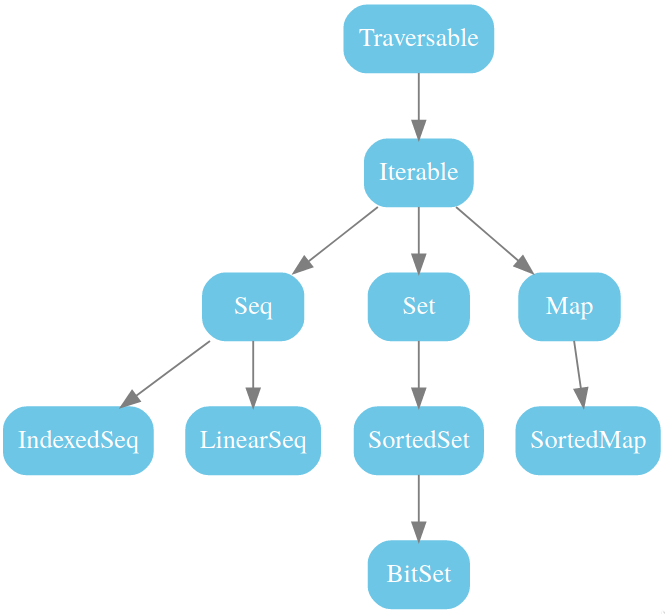
\includegraphics[width=1.0\textwidth]{../img/collection/collection-traits}
\end{Slide}
\noindent Läs mer om Scalas samlingar här: \\ 
\url{http://docs.scala-lang.org/overviews/collections/overview}


\begin{Slide}{Hierarki av samlingstyper i \texttt{scala.collection}}

\begin{multicols}{2}
\begin{tikzpicture}[sibling distance=6.1em,->,>=stealth', inner sep=3pt, %scale=0.5, 
  every node/.style = {shape=rectangle, draw, align=center,font=\small\ttfamily},
  class/.style = {fill=blue!20},
  trait/.style = {rounded corners, fill=red!20}]
  \node[trait] {Traversable}
    child { node[trait] {Iterable} 
      child { node[trait] {Seq} 
       }
      child { node[trait] {Set} 
      }
      child { node[trait] {Map} 
      }
    };
\end{tikzpicture}

\columnbreak
 
{\SlideFontTiny 

\code{Traversable} har metoder som är implementerade med hjälp av: \\
\code{def foreach[U](f: Elem => U): Unit}\\

\vspace{1em}\code{Iterable} har metoder som är implementerade med hjälp av: \\
\code{def iterator: Iterator[A] } 

}

\begin{itemize}\SlideFontTiny 
\item[] \code{Seq}: ordnade i sekvens
\item[] \code{Set}: unika element
\item[] \code{Map}: par av (nyckel, värde)
\end{itemize}


\end{multicols}

{\SlideFontSmall Samlingen \Emph{\texttt{Vector}} är en \code{Seq} som är en \code{Iterable} som är en \code{Traversable}.}
\end{Slide}

\begin{Slide}{Använda \texttt{iterator}}\SlideFontSmall
Med en \code{iterator} kan man \Emph{iterera} med \code{while} över alla element, men endast \Alert{en   gång}; sedan är iteratorn ''förbrukad''. (Men man kan be om en ny.)
\begin{REPL}
scala> val xs = Vector(1,2,3,4)
xs: scala.collection.immutable.Vector[Int] = Vector(1, 2, 3, 4)

scala> val it = xs.iterator
it: scala.collection.immutable.VectorIterator[Int] = non-empty iterator

scala> while (it.hasNext) print(it.next)
1234

scala> it.hasNext
res1: Boolean = false

scala> it.next
java.util.NoSuchElementException: reached iterator end
  at scala.collection.immutable.VectorIterator.next(Vector.scala:674)
\end{REPL}
\Emph{Normalt} behöver man \Alert{inte} använda \code{iterator}: det finns oftast färdiga metoder som gör det man vill, till exempel \code{foreach}, \code{map}, \code{sum}, \code{min} etc.
\end{Slide}

\begin{Slide}{Några användbara metoder på samlingar}\SlideFontTiny
\begin{tabular}{r r l}\hline
\texttt{\Emph{Traversable}} 
  & \code|xs.size| & antal elementet \\
  & \code|xs.head| & första elementet \\
  & \code|xs.last| & sista elementet \\
  & \code|xs.take(n)| & ny samling med de första n elementet \\
  & \code|xs.drop(n)| & ny samling utan de första n elementet \\
  & \code|xs.foreach(f)| & gör \code|f| på alla element, returtyp \code|Unit|\\
  & \code|xs.map(f)| & gör \code|f| på alla element, ger ny samling \\
  & \code|xs.filter(p)| & ny samling med bara de element där p är sant\\
  & \code|xs.groupBy(f)| & ger en \code|Map| som grupperar värdena enligt f\\ 
  & \code|xs.mkString(",")| & en kommaseparerad sträng med alla element\\ \hline
    
\texttt{\Emph{Iterable}} 
  & \code|xs.zip(ys)| & ny samling med par (x, y); ''zippa ihop'' xs och ys \\
  & \code|xs.zipWithIndex| & ger en \code|Map| med par (x, index för x) \\
  & \code|xs.sliding(n)| & ny samling av samlingar genom glidande ''fönster''\\ \hline

\texttt{\Emph{Seq}} 
  & \code|xs.length| & samma som \code|xs.size| \\
  & \code|xs :+ x| & ny samling med x sist efter xs \\
  & \code|x +: xs| & ny samling med x före xs \\ \hline
  
\end{tabular}

\pause
\vspace{0.5em}\Emph{Minnesregel} för \code{+:} och \code{:+  } \Alert{Colon on the collection side}

\pause
Prova fler samlingsmetoder ur snabbreferensen: ~~\url{http://cs.lth.se/quickref}
\end{Slide}



\begin{Slide}{Använda samlingsmetoder}
\begin{REPL}
scala> val tal = Vector(1,4,7,9,42)
tal: scala.collection.immutable.Vector[Int] = Vector(1, 4, 7, 9, 42)

scala> val jämna = tal.filter(_ % 2 == 0)
jämna: scala.collection.immutable.Vector[Int] = Vector(4, 42)

scala> val xs = Vector(("Kim","Smith"), ("Kim", "Jones"), ("Robin", "Smith"))
xs: scala.collection.immutable.Vector[(String, String)] = Vector((Kim,Smith), (Kim,Jones), (Robin,Smith))

scala> val grupperaEfterFörnamn = xs.groupBy(_._1)
grupperaEfterFörnamn: Map[String,Vector[(String, String)]] = 
Map(Kim -> Vector((Kim,Smith), (Kim,Jones)), Robin -> Vector((Robin,Smith)))

scala> val grupperaEfterEfternamn = xs.groupBy(_._2)
grupperaEfterEfternamn: Map[String,Vector[(String, String)]] = 
Map(Jones -> Vector((Kim,Jones)), Smith -> Vector((Kim,Smith), (Robin,Smith)))

\end{REPL}
\end{Slide}




\begin{Slide}{Mer specifik samlingstyper i \texttt{scala.collection}}
Det finns \Alert{mer specifika} \Emph{subtyper} av \code{Seq}, \code{Set} och \code{Map}:
\\ \vspace{1em}

\begin{tikzpicture}[sibling distance=5.8em,->,>=stealth', inner sep=3pt, %scale=0.5, 
  every node/.style = {shape=rectangle, draw, align=center,font=\small\ttfamily},
  class/.style = {fill=blue!20},
  trait/.style = {rounded corners, fill=red!20}]
  \node[trait] {Traversable}
    child { node[trait] {Iterable} 
      child { node[trait, xshift=-2.4cm] {Seq} 
        child { node[trait] {IndexedSeq} }
        child { node[trait] {LinearSeq} }
       }
      child { node[trait, yshift=-0.0cm] {Set} 
        child { node[trait] {SortedSet} }
        child { node[trait] {BitSet} }
      }
      child { node[trait, xshift=1.0cm] {Map} 
        child { node[trait] {SortedMap} }
      }
    };
\end{tikzpicture}

\vspace{0.5em}
\Emph{\texttt{Vector}} är en \Alert{\texttt{IndexedSeq}} medan
\Emph{\texttt{List}} är en \Alert{\texttt{LinearSeq}}.
\end{Slide}

\begin{Slide}{Några oföränderliga och förändringsbara sekvenssamlingar}\SlideFontSmall
\begin{tabular}{r l l}
\texttt{scala.collection.\Emph{immutable}.Seq.} & & \\
 & \code|IndexedSeq.| & \\
 & & \Emph{\texttt{Vector}} \\
 & & \Emph{\texttt{Range}} \\
 & \code|LinearSeq.| & \\
 & & \Emph{\texttt{List}} \\
   & & \Emph{\texttt{Queue}} \\

\texttt{scala.collection.\Alert{mutable}.Seq.} & & \\
 & \code|IndexedSeq.| & \\
 & & \Alert{\texttt{ArrayBuffer}} \\
 & & \Alert{\texttt{StringBuilder}} \\
 & \code|LinearSeq.| & \\
 & & \Alert{\texttt{ListBuffer}} \\
   & & \Alert{\texttt{Queue}} \\
\end{tabular}

Studera samlingars egenskaper här: \href{http://docs.scala-lang.org/overviews/collections/overview}{docs.scala-lang.org/overviews/collections/overview}
\end{Slide}


\begin{Slide}{scala.collection.immutable}
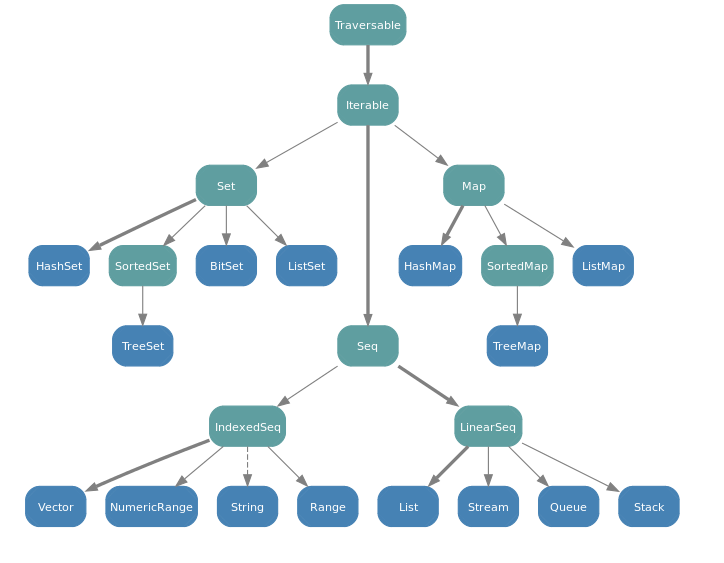
\includegraphics[width=0.82\textwidth]{../img/collection/collection-immutable}
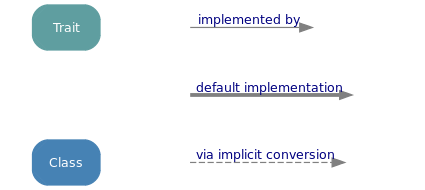
\includegraphics[width=0.33\textwidth]{../img/collection/collection-legend}
\end{Slide}


\begin{Slide}{scala.collection.mutable}
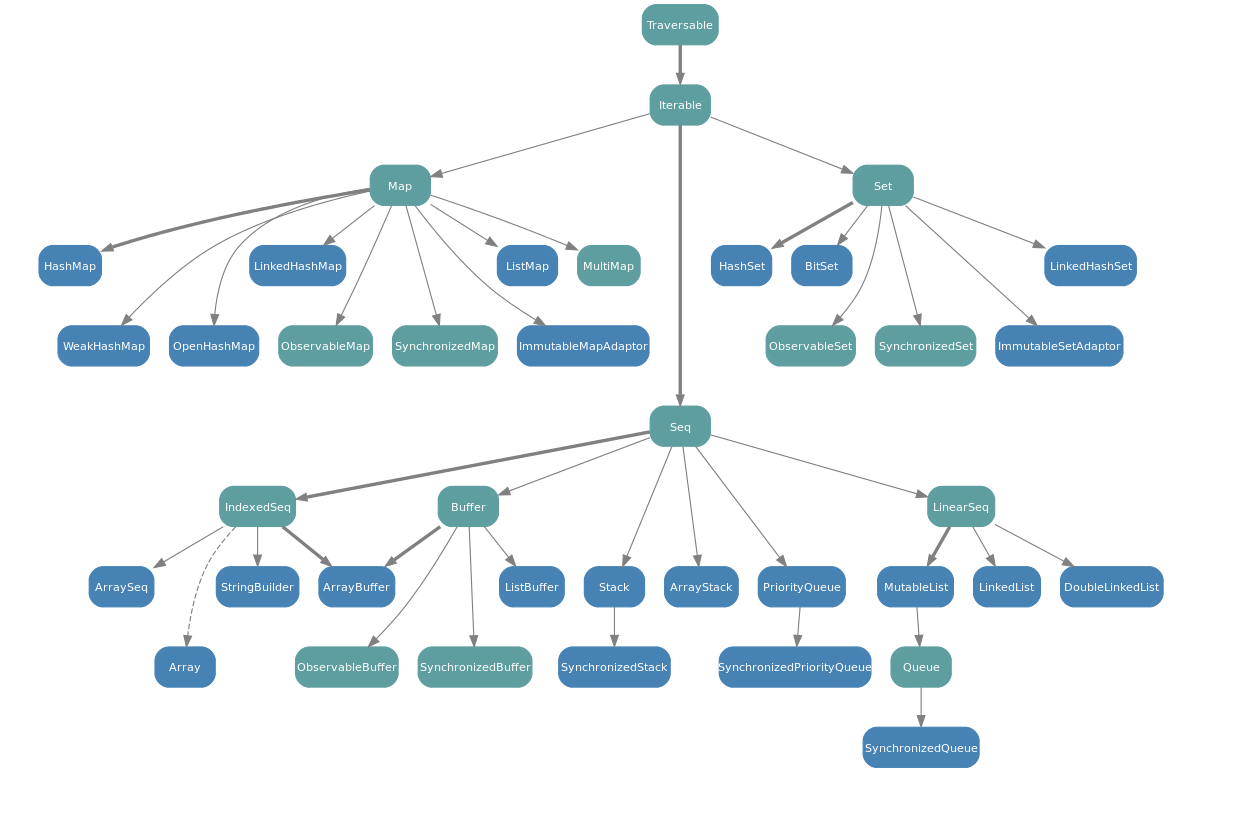
\includegraphics[width=1.05\textwidth]{../img/collection/collection-mutable}
\end{Slide}


\begin{Slide}{Strängar är implicit en \texttt{IndexedSeq[Char]}}\SlideFontSmall
Det finns en så kallad \Emph{implicit konvertering} mellan \code{String} och \code{IndexedSeq[Char]} vilket gör att \Alert{alla samlingsmetoder på \texttt{Seq} även funkar på strängar} och även flera andra smidiga strängmetoder erbjuds \Alert{utöver} de som finns i \href{http://docs.oracle.com/javase/8/docs/api/java/lang/String.html}{\code{java.lang.String}} genom klassen \href{http://www.scala-lang.org/api/current/#scala.collection.immutable.StringOps}{\code{StringOps}}.

\vspace{0.5em}
\begin{REPLnonum}
scala> "hej".  //tryck på TAB och se alla strängmetoder
\end{REPLnonum}
Detta är en stor fördel med Scala jämfört med många andra språk, som har strängar som inte kan allt som andra sekvenssamlingar kan.
\end{Slide}


\begin{Slide}{\texttt{Vector} eller \texttt{List}?}\SlideFontTiny
{\href{http://stackoverflow.com/questions/6928327/when-should-i-choose-vector-in-scala}{stackoverflow.com/questions/6928327/when-should-i-choose-vector-in-scala}}

\begin{enumerate}
\item If we only need to transform sequences by operations like map, filter, fold etc: basically it does not matter, we should program our algorithm generically and might even benefit from accepting parallel sequences. For sequential operations List is probably a bit faster. But you should benchmark it if you have to optimize.

\item If we need a lot of random access and different updates, so we should use vector, list will be prohibitively slow.

\item If we operate on lists in a classical functional way, building them by prepending and iterating by recursive decomposition: use list, vector will be slower by a factor 10-100 or more.

\item If we have an performance critical algorithm that is basically imperative and does a lot of random access on a list, something like in place quick-sort: use an imperative data structure, e.g. ArrayBuffer, locally and copy your data from and to it.
\end{enumerate}
{\href{http://stackoverflow.com/questions/20612729/how-does-scalas-vector-work}{stackoverflow.com/questions/20612729/how-does-scalas-vector-work}}\\
Mer om tids- och minneskomplexitet i fördjupningskursen och senare kurser.
\end{Slide}



\begin{Slide}{Mängd: snabb innehållstest, garanterat dubblettfri}\SlideFontSmall
En \Emph{mängd} \Eng{set} är en samling som \Alert{inte} kan innehålla \Alert{dubbletter} och som är snabb på att avgöra om ett element \Alert{finns eller inte} i mängden.

\begin{REPL}
scala> var veg = Set.empty[String]
veg: scala.collection.immutable.Set[String] = Set()

scala> veg = veg + "Gurka"
veg: scala.collection.immutable.Set[String] = Set(Gurka)

scala> veg = veg ++ Set("Broccoli", "Tomat", "Gurka")
veg: scala.collection.immutable.Set[String] = Set(Gurka, Broccoli, Tomat)

scala> veg.contains("Gurka")
res0: Boolean = true

scala> veg.apply("Gurka")   // samma som contains
res1: Boolean = true

scala> veg("Morot")
res2: Boolean = false
\end{REPL}

\end{Slide}

\begin{Slide}{Den fantastiska nyckel-värde-tabellen \texttt{Map}}\SlideFontSmall
\begin{itemize}
\item En \Emph{nyckel-värde-tabell} \Eng{key-value table} är en slags generaliserad vektor där man kan ''indexera'' med godtycklig typ. 

\item Kallas öven \href{https://sv.wikipedia.org/wiki/Hashtabell}{\Emph{hashtabell}} \Eng{hash table}, \Emph{lexikon} \Eng{dictionary} eller kort och gott \Emph{mapp} \Eng{map},

\item En hashtabell är en \Emph{samling av par}, där varje par består av en \Alert{unik} \Emph{nyckel} och ett tillhörande \Emph{värde}. 

\item Om man vet nyckeln kan man få fram värdet \Alert{snabbt}, på liknande sätt som indexering sker i en vektor om man vet heltalsindex. 

\item Denna datastruktur är \Alert{mycket användbar} och liknar en enkel databas.
\end{itemize}
\begin{REPL}
scala> val födelse = Map("C" -> 1972,  "C++" -> 1983, "C#" -> 2000, 
  "Scala" -> 2004, "Java" -> 1995, "Javascript" -> 1995, "Python" -> 1991)

födelse: scala.collection.immutable.Map[String,Int] = Map(Scala -> 2004, C# -> 2000, Python -> 1991, Javascript -> 1995, C -> 1972, C++ -> 1983, Java -> 1995)
  
scala> födelse.apply("Scala")
res0: Int = 2004

scala> födelse("Java")
res1: Int = 1995

\end{REPL}
\end{Slide}

\begin{Slide}{Exempel nyckel-värde-tabell}
\begin{REPL}
scala> val färg = Map("gurka" -> "grön", "tomat"->"röd", "aubergine"->"lila")
färg: scala.collection.immutable.Map[String,String] = 
  Map(gurka -> grön, tomat -> röd, aubergine -> lila)

scala> färg("gurka")
res0: String = grön

scala> färg.keySet
res1: scala.collection.immutable.Set[String] = Set(gurka, tomat, aubergine)

scala> val ärGrönSak = färg.map(elem => (elem._1, elem._2 == "grön"))
ärGrönSak: Map[String,Boolean] = Map(gurka -> true, tomat -> false, aubergine -> false)

scala> val baklängesFärg = färg.mapValues(s => s.reverse)
baklängesFärg: Map[String,String] = Map(gurka -> nörg, tomat -> dör, aubergine -> alil)

\end{REPL}
\begin{itemize}
\item \code{xs.keySet} ger en mängd av alla nycklar
\item \code{xs.map(f)} mappar funktionen f på alla par av (key, value)
\item \code{xs.mapValues(f)} mappar funktionen f på alla värden 
\end{itemize}

\end{Slide}

\begin{Slide}{Metoderna zipWithIndex, groupBy och mapValues}
\begin{REPL}
scala> val högaKort = Vector("Knekt", "Dam", "Kung", "Äss")

scala> val kortIndex = högaKort.zipWithIndex.toMap
kortIndex: Map[String,Int] = Map(Knekt -> 0, Dam -> 1, Kung -> 2, Äss -> 3)

scala> kortIndex("Kung") > kortIndex("Knekt") 
res0: Boolean = true

scala> val xs = Vector(("Kim","Smith"), ("Kim", "Jones"), ("Robin", "Smith"))
xs: Vector[(String, String)] = Vector((Kim,Smith), (Kim,Jones), (Robin,Smith))

scala> val grupperaEfterFörnamn = xs.groupBy(_._1)
grupperaEfterFörnamn: Map[String,Vector[(String, String)]] = 
Map(Kim -> Vector((Kim,Smith), (Kim,Jones)), Robin -> Vector((Robin,Smith)))

scala> val grupperaEfterEfternamn = xs.groupBy(_._2)
grupperaEfterEfternamn: Map[String,Vector[(String, String)]] = 
Map(Jones -> Vector((Kim,Jones)), Smith -> Vector((Kim,Smith), (Robin,Smith)))

scala> val frekvens = xs.groupBy(_._1).mapValues(_.size)
frekvens: Map[String,Int] = Map(Kim -> 2, Robin -> 1)
\end{REPL}
\end{Slide}


\begin{Slide}{Speciella metoder på förändringsbara samlingar}\SlideFontSmall
Både \code{Set} och \code{Map} finns i \Alert{förändringsbara} varianter med extra metoder för uppdatering av innehållet ''på plats'' utan att nya samlingar skapas.
\begin{REPL}
scala> import scala.collection.mutable

scala> val ms = mutable.Set.empty[Int]
ms: scala.collection.mutable.Set[Int] = Set()

scala> ms += 42
res0: ms.type = Set(42)

scala> ms += (1, 2, 3, 1, 2, 3); ms -= 1
res1: ms.type = Set(2, 42, 3)

scala> ms.mkString("Mängd: ", ", ", s" Antal: ${ms.size}")
res2: String = Mängd: 1, 2, 42, 3 Antal: 4

scala> val ordpar = mutable.Map.empty[String, String]
scala> ordpar += ("hej" -> "svejs", "abra" -> "kadabra", "ada" -> "lovelace")
scala> println(ordpar("abra"))
kadabra
\end{REPL}
\end{Slide}

\begin{Slide}{Fler exempel på samlingsmetoder}
Exempel: räkna bokstäver i ord.  \\
Undersök vad som händer i REPL:
\begin{Code}[basicstyle=\SlideFontSize{9}{13}\ttfamily]
val ord = "sex laxar i en laxask sju sjösjuka sjömän" 
val uppdelad = ord.split(' ').toVector
val ordlängd = uppdelad.map(_.length)
val ordlängdMap = uppdelad.map(s => (s, s.size)).toMap
val grupperaEfterFörstaBokstav = uppdelad.groupBy(s => s(0))
val bokstäver = ord.toVector.filter(_ != ' ')
val antalX = bokstäver.count(_ == 'x')
val grupperade = bokstäver.groupBy(ch => ch)
val antal = grupperade.map(kv => (kv._1, kv._2.size))
val sorterat = antal.toVector.sortBy(_._2)
val vanligast = antal.maxBy(_._2)
\end{Code}
\end{Slide}


\begin{Slide}{Jobba med föränderlig samling lokalt; \\ returnera oföränderlig samling när du är klar}
\SlideFontSmall
Om du vill implementera en imperativ algoritm med en föränderlig samling:\\ 
Gör gärna detta \Alert{lokalt} i en \Alert{förändringsbar} samling och returnera sedan en \Emph{oföränderlig} samling, genom att köra t.ex. \code{toSet} på en mängd, eller \code{toMap} på en hashtabell, eller \code{toVector} på en \code{ArrayBuffer} eller \code{Array}.

\begin{REPL}
scala> :paste
def kastaTärningTillsAllaUtfallUtomEtt(sidor: Int = 6) = {
  val s = scala.collection.mutable.Set.empty[Int]
  var n = 0
  while (s.size < sidor - 1) {
    s += (math.random * sidor + 1).toInt
    n += 1
  }
  (n, s.toSet)
}
scala> kastaTärningTillsAllaUtfallUtomEtt()
res0: (Int, scala.collection.immutable.Set[Int]) = (13,Set(5, 1, 6, 2, 3))

\end{REPL}

\end{Slide}






%!TEX encoding = UTF-8 Unicode
%!TEX root = ../lect-w07.tex

\Subsection{Integrerad utvecklingsmiljö (IDE)}

\begin{Slide}{Välja IDE}\SlideFontSmall
\begin{itemize}
\item En \Emph{integrerad utvecklingsmiljö} \Eng{Integrated Development Environment, IDE} innehåller \\ editor + kompilator + debugger + en massa annat\\och gör utvecklingen enklare när man lärt sig alla finesser.

\item Läs om vad en IDE kan göra i appendix D\\(ingår i labbförberedelserna för lab \texttt{pirates}).

\pause

\item På LTH:s datorer finns två populära IDE installerade:
\begin{enumerate}\SlideFontSmall
\item \Emph{Eclipse} med plugin \Emph{ScalaIDE} förinstallerad
\begin{REPL}[numbers=none]
$ scalaide
\end{REPL}
\item \Emph{IntelliJ IDEA} (välj installera Scala-plugin när du kör första gången)
\begin{REPL}[numbers=none]
$ idea
\end{REPL}

\end{enumerate}
Läs mer om dessa i appendix D innan du väljer vilken du vill lära dig. Där står även hur du installerar dem på din egen dator. \\Flest handledare har störst vana vid Eclipse.
\end{itemize}
\end{Slide}

\begin{Slide}{Eclipse med ScalaIDE}
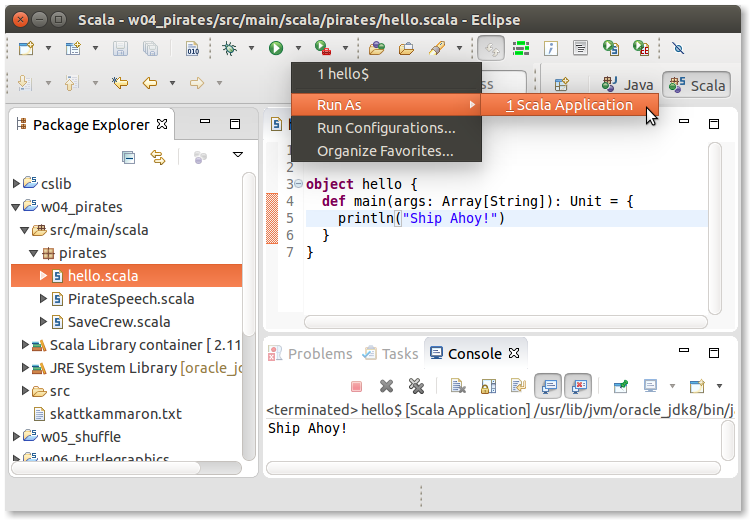
\includegraphics[width=\textwidth]{../img/eclipse/eclipse-pirates-hello.png}
\end{Slide}


\begin{Slide}{IntelliJ IDEA med Scala-plugin}
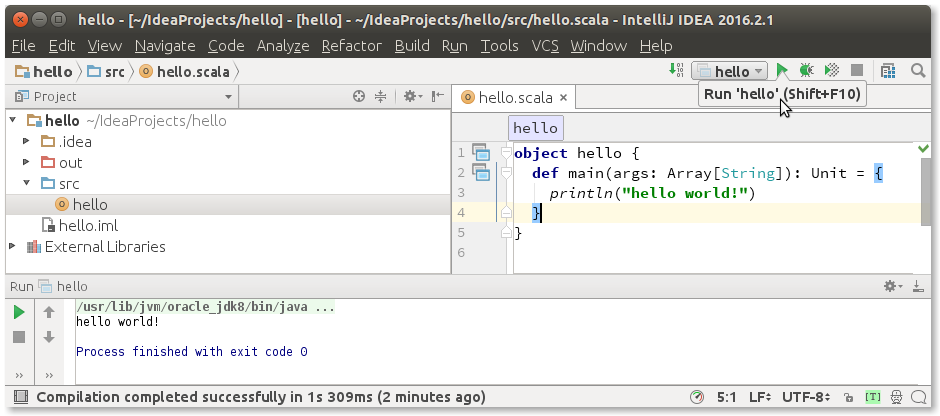
\includegraphics[width=\textwidth]{../img/intellij/idea-hello.png}
\end{Slide}

\ifkompendium\else

\begin{Slide}{Denna veckas övning: \texttt{data}}
\begin{itemize}\SlideFontTiny
%!TEX encoding = UTF-8 Unicode
%!TEX root = ../compendium2.tex

\item Kunna skapa och använda tupler, som variabelvärden, parametrar och returvärden.

\item Förstå skillnaden mellan ett objekt och en klass och kunna förklara betydelsen av begreppet instans.

\item Kunna skapa och använda attribut som medlemmar i objekt och klasser och som som klassparametrar.

\item Beskriva innebörden av och syftet med att ett attribut är privat.

\item Kunna byta ut implementationen av metoden \code{toString}.

\item Kunna skapa och använda en objektfabrik med metoden \code{apply}.

\item Kunna skapa och använda en enkel case-klass.

\item Kunna använda operatornotation och förklara relationen till punktnotation.

\item Förstå konsekvensen av uppdatering av föränderlig data i samband med multipla referenser.

\item Känna till och kunna använda några grundläggande metoder på samlingar.

\item Känna till den principiella skillnaden mellan \code{List} och \code{Vector}.

\item Kunna skapa och använda en oföränderlig mängd med klassen \code{Set}.

\item Förstå skillnaden mellan en mängd och en sekvens.

\item Kunna skapa och använda en nyckel-värde-tabell, \code{Map}.

\item Förstå likheter och skillnader mellan en \code{Map} och en \code{Vector}.

\end{itemize}
\end{Slide}

\begin{Slide}{Denna veckas laboration: \texttt{pirates}}
\begin{itemize}\SlideFontSmall
%!TEX encoding = UTF-8 Unicode
%!TEX root = ../compendium2.tex

%\item Kunna använda en integrerad utvecklingsmiljö (IDE).
%\item Kunna använda färdiga funktioner för att läsa till, och skriva från, textfil.
%\item Kunna använda enkla case-klasser.
%\item Kunna skapa och använda enkla klasser med föränderlig data.
\item Kunna skapa och använda nyckel-värde-tabeller med samlingstypen \code{Map}.
\item Kunna skapa och använda mängder med samlingstypen \code{Set}.
\item Förstå skillnaden mellan en ordnad sekvens och en mängd.
\item Förstå likheter och skillnader mellan en sekvens av par och en nyckel-värde-tabell. 
%\item Kunna skapa en ny samling från en befintlig samling.
%\item Förstå skillnaden mellan kompileringsfel och exekveringsfel.
%\item Kunna felsöka i små program med hjälp av utskrifter.
%\item Kunna felsöka i små program med hjälp av en debugger i en IDE.

\end{itemize}
\end{Slide}

\fi


%!TEX encoding = UTF-8 Unicode

%!TEX root = ../compendium1.tex

%!TEX encoding = UTF-8 Unicode
\chapter{Matriser, typparametrar}\label{chapter:W08}
Begrepp som ingår i denna veckas studier:
\begin{itemize}[noitemsep,label={$\square$},leftmargin=*]
\item matris
\item nästlad samling
\item nästlad for-sats
\item typparameter
\item generisk funktion
\item generisk klass
\item fri vs bunden typparameter
\item generiska datastrukturer
\item generiska samlingar i Scala\end{itemize}

\clearpage\section{Teori}
%!TEX encoding = UTF-8 Unicode
%!TEX root = ../lect-w08.tex

%%%

\Subsection{Veckans labb: \texttt{life}}

\begin{Slide}{Veckans labb: \texttt{life}}
\begin{minipage}{0.52\textwidth}
  \setlength{\leftmargini}{0pt}

\begin{itemize}
  \SlideFontSmall
\item Universum är en binär matris av \Emph{celler} där \Emph{levande} celler representeras med \code{true} och \Alert{döda} med \code{false}.
\item Följande regler gäller för \Emph{nästa generation} celler i universum:
\begin{itemize}\SlideFontTiny
  \item \textbf{Fortlevnad}: en levande cell med 2 eller 3 grannar \Emph{lever vidare}
  \item \textbf{Död}: en levande cell med färre än 2 eller fler än 3 grannar \Alert{dör}
  \item \textbf{Födelse}: en död cell med exakt tre grannar föds
\end{itemize}
\item Övning \code{matrices} uppgift 5: skapa en generisk \code{case class Matrix[T]}
\item På labben: använd \code{Matrix[Boolean]}
\end{itemize}

\end{minipage}%
\begin{minipage}{0.5\textwidth}
  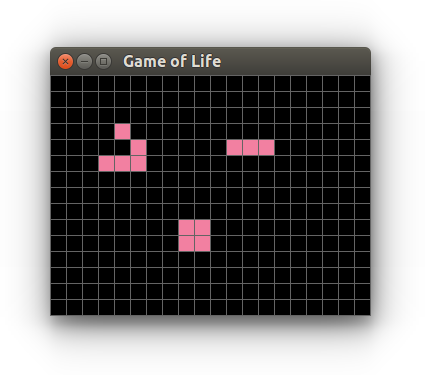
\includegraphics[width=1.0\textwidth]{../img/glider-blinker-block}

  \begin{itemize}\SlideFontTiny
  \item Du ska simulera \emph{Game of Life} i ett \code{introprog.PixelWindow}
  \item Fördjupning:\\{\SlideFontTiny\url{https://en.wikipedia.org/wiki/Conway%27s_Game_of_Life}}
  \end{itemize}
\end{minipage}%

\end{Slide}






\Subsection{Matriser}

\begin{Slide}{Vad är en matris?}\SlideFontSmall
\begin{itemize}

\item En \Emph{matris} inom \Alert{matematiken} innehåller \Emph{rader} och \Emph{kolumner}\footnote{även kallade \emph{kolonner}} med tal.

\item I en \Alert{matematisk} matris har alla rader \Emph{lika många} element och

\item även alla kolumner har \Emph{lika många} element.

\item En matris av dimension $2\times{}5$ har $2 \cdot 5 = 10$ stycken element.

\item Exempel på en matematisk matris av dimension $2\times{}5$:
\[
M_{2,5}=
  \begin{pmatrix}
    5 & 2 & 42 & 4 & 5 \\
    3 & 4 & 18 & 6 & 7
  \end{pmatrix}
\]
\end{itemize}
\end{Slide}

\begin{Slide}{Indexering i en matris}\SlideFontSmall
\begin{itemize}

  \item En matris av dimension $m\times{}n$ har $m \cdot n$ stycken element.

  \item En matris $A_{m,n}$ av dimension $m\times{}n$ ritas inom matematiken ofta så här:

  \[
  A_{m,n} =
   \begin{pmatrix}
    a_{1,1} & a_{1,2} & \cdots & a_{1,n} \\
    a_{2,1} & a_{2,2} & \cdots & a_{2,n} \\
    \vdots  & \vdots  & \ddots & \vdots  \\
    a_{m,1} & a_{m,2} & \cdots & a_{m,n}
   \end{pmatrix}
  \]


\item Matrisindexering inom matematiken sker ofta från $1$, men ofta från $0$ i datorprogram.

\item Vad har talet $42$ för index i matrisen $M_{2,5}$ nedan?
\begin{itemize}\SlideFontTiny
  \item[--] Inom matematiken?
  \item[--] I Scala och Java och många andra språk?

  \[
  M_{2,5}=
    \begin{pmatrix}
      5 & 2 & 42 & 4 & 5 \\
      3 & 4 & 18 & 6 & 7
    \end{pmatrix}
  \]
\end{itemize}
\end{itemize}
\end{Slide}

\begin{Slide}{En matris med array av arrayer}
Inom programmering används ordet \Emph{matris} ofta för att beteckna en \Alert{nästlad struktur} i två dimensioner, till exempel en instans av typen \code{Array[Array[Int]]}
\begin{REPL}
scala> val xss = Array(Array(5,2,42,4,5),Array(3,4,18,6,7))
xss: Array[Array[Int]] = Array(Array(5, 2, 42, 4, 5), Array(3, 4, 18, 6, 7))
\end{REPL}
\pause
Man indexerar i en nästlad sekvens med upprepad \code{apply}:
\begin{REPL}
scala> xss(0)(2)
res0: ???                   // Vad är typ och värde?

scala> xss.apply(0).apply(2)
res1: ???                   // Vad är typ och värde?

scala> xss(0)
res2: ???                   // Vad är typ och värde?
\end{REPL}

\end{Slide}

\begin{Slide}{En matris med array av arrayer}
Inom programmering används ordet \Emph{matris} ofta för att beteckna en \Alert{nästlad struktur} i två dimensioner, till exempel en instans av typen \code{Array[Array[Int]]}
\begin{REPL}
scala> val xss = Array(Array(5,2,42,4,5),Array(3,4,18,6,7))
xss: Array[Array[Int]] = Array(Array(5, 2, 42, 4, 5), Array(3, 4, 18, 6, 7))
\end{REPL}

Man indexerar i en nästlad sekvens med upprepad \code{apply}:
\begin{REPL}
scala> xss(0)(2)
res0: Int = 42

scala> xss.apply(0).apply(2)
res1: Int = 42

scala> xss(0)
res2: Array[Int] = Array(5, 2, 42, 4, 5)
\end{REPL}
\end{Slide}

\begin{Slide}{Uppdatering av en förändringsbar nästlad struktur}
Man kan förändra en array av arrayer ''på plats'' med tilldelning:
\begin{REPL}
scala> val xss = Array(Array(5,2,42,4,5),Array(3,4,18,6,7))

scala> xss(0)(0) = 100

scala> xss
res0: ???

scala> xss(0)(2) = xss(0)(2) - 1

scala> xss
res1: ???

scala> xss(1) = Array.fill(5)(-1)

scala> xss
res2: ???
\end{REPL}
\end{Slide}

\begin{Slide}{Uppdatering av en förändringsbar nästlad struktur}
Man kan förändra en array av arrayer ''på plats'' med tilldelning:
\begin{REPL}
scala> val xss = Array(Array(5,2,42,4,5),Array(3,4,18,6,7))

scala> xss(0)(0) = 100

scala> xss
res0: Array[Array[Int]]=Array(Array(100, 2, 42, 4, 5), Array(3, 4, 18, 6, 7))

scala> xss(0)(2) = xss(0)(2) - 1

scala> xss
res1: Array[Array[Int]]=Array(Array(100, 2, 41, 4, 5), Array(3, 4, 18, 6, 7))

scala> xss(1) = Array.fill(5)(-1)

scala> xss
res2: Array[Array[Int]]=Array(Array(100, 2, 41, 4, 5), Array(-1,-1,-1,-1,-1))
\end{REPL}
\end{Slide}

\begin{Slide}{Några olika sätt att skapa förändringsbara matriser}\SlideFontSmall
Det jobbiga, primitiva sättet:
\begin{REPL}
scala> val xs = new Array[Array[Int]](2)
xs: Array[Array[Int]] = Array(null, null)

scala> for (i <- xs.indices) {xs(i) = new Array[Int](5)}

scala> xs
res0: Array[Array[Int]] = Array(Array(0, 0, 0, 0, 0), Array(0, 0, 0, 0, 0))

scala> println(xs)
[[I@196a99d0
\end{REPL}
Enklare sätt:
\begin{REPL}
scala> val xs = Array.ofDim[Int](2,5)
xs: Array[Array[Int]] = Array(Array(0, 0, 0, 0, 0), Array(0, 0, 0, 0, 0))
\end{REPL}
Enklare och tydligare sätt, där initialvärdet anges explicit:
\begin{REPL}
scala> Array.fill(2,5)(0)
res37: Array[Array[Int]] = Array(Array(0, 0, 0, 0, 0), Array(0, 0, 0, 0, 0))
\end{REPL}

\end{Slide}

\begin{Slide}{Exempel på skapande av oföränderlig nästlad struktur}\SlideFontSmall
Om du kan beräkna initialvärde direkt, använd \code{Vector.fill}:\\
{\SlideFontTiny\code{def fill[A](n1: Int, n2: Int)(elem: => A): Vector[Vector[A]]}}
\begin{REPL}
scala> Vector.fill(2,5)(scala.util.Random.nextInt(6) + 1)
res0:
  typ???
  värde???

\end{REPL}
Om du kan beräkna initialvärde ur index, använd \code{Vector.tabulate}:\\
{\SlideFontTiny\code{def tabulate[A](n1: Int, n2: Int)(f: (Int, Int) => A): Vector[Vector[A]]}}
\begin{REPL}
scala> Vector.tabulate(5,2)((x,y) => x + y + 1)
res1:
  typ???
  värde???

\end{REPL}
\end{Slide}

\begin{Slide}{Exempel på skapande av oföränderlig nästlad struktur}\SlideFontSmall
Om du kan beräkna initialvärde direkt, använd \code{Vector.fill}:\\
{\SlideFontTiny\code{def fill[A](n1: Int, n2: Int)(elem: => A): Vector[Vector[A]]}}
\begin{REPL}
scala> Vector.fill(2,5)(scala.util.Random.nextInt(6) + 1)
res0:
  scala.collection.immutable.Vector[scala.collection.immutable.Vector[Int]] =
  Vector(Vector(1, 2, 6, 2, 1), Vector(1, 4, 3, 3, 2))

\end{REPL}
Om du kan beräkna initialvärde ur index, använd \code{Vector.tabulate}:\\
{\SlideFontTiny\code{def tabulate[A](n1: Int, n2: Int)(f: (Int, Int) => A): Vector[Vector[A]]}}
\begin{REPL}
scala> Vector.tabulate(5,2)((x,y) => x + y + 1)
res1:
  scala.collection.immutable.Vector[scala.collection.immutable.Vector[Int]] =
  Vector(Vector(1,2), Vector(2,3), Vector(3,4), Vector(4,5), Vector(5,	6))

\end{REPL}
\end{Slide}



\begin{Slide}{Uppdatering av en oföränderlig nästlad struktur}\SlideFontSmall
Uppdatering av endimensionell struktur med \code{xs.updated}:\\
{\SlideFontTiny\code{def updated[A](index: Int, elem: A): Vector[A]} }
\begin{REPL}
scala> var xs = Vector.tabulate(5)(x => x + 1)
xs: typ??? = värde???

scala> xs = xs.updated(1, 42)
xs: typ??? = värde???
\end{REPL}

Uppdatering av nästlad struktur i två dimensioner:
\begin{REPL}
scala> var xss = Vector.tabulate(2, 5)((x,y) => x + y + 1)
xss:
  typ??? =
  värde???

scala> xss = xss.updated(0, xss(0).updated(1, 42))
xss:
  typ??? =
  värde???
\end{REPL}

\end{Slide}



\begin{Slide}{Uppdatering av en oföränderlig nästlad struktur}\SlideFontSmall
Uppdatering av endimensionell struktur med \code{xs.updated}:\\
{\SlideFontTiny\code{def updated[A](index: Int, elem: A): Vector[A]} }
\begin{REPL}
scala> var xs = Vector.tabulate(5)(x => x + 1)
xs: scala.collection.immutable.Vector[Int] = Vector(1, 2, 3, 4, 5)

scala> xs = xs.updated(1, 42)
xs: scala.collection.immutable.Vector[Int] = Vector(1, 42, 3, 4, 5)
\end{REPL}

Uppdatering av nästlad struktur i två dimensioner:
\begin{REPL}
scala> var xss = Vector.tabulate(2, 5)((x,y) => x + y + 1)
xss:
  scala.collection.immutable.Vector[scala.collection.immutable.Vector[Int]] =
  Vector(Vector(1, 2, 3, 4, 5), Vector(2, 3, 4, 5, 6))

scala> xss = xss.updated(0, xss(0).updated(1, 42))
xss:
  scala.collection.immutable.Vector[scala.collection.immutable.Vector[Int]] =
  Vector(Vector(1, 42, 3, 4, 5), Vector(2, 3, 4, 5, 6))
\end{REPL}

\end{Slide}


\begin{Slide}{Iterera över nästlad struktur: for-sats}\SlideFontSmall
Iterera med nästlad for-sats:
\begin{REPL}
scala> val xss = Vector.tabulate(2,5)((x,y) => x + y + 1)

scala> for (???) {
         for (???) {
           print(xss(i)(j) + " ")
         }
         println
       }

1 2 3 4 5
2 3 4 5 6
\end{REPL}
\end{Slide}

\begin{Slide}{Iterera över nästlad struktur: for-sats}\SlideFontSmall
Iterera med nästlad for-sats:
\begin{REPL}
scala> val xss = Vector.tabulate(2,5)((x,y) => x + y + 1)

scala> for (i <- xss.indices) {
         for (j <- xss(i).indices) {
           print(xss(i)(j) + " ")
         }
         println
       }

1 2 3 4 5
2 3 4 5 6
\end{REPL}
\end{Slide}


\begin{Slide}{Övningsexempel: Yatzy}\SlideFontSmall
Skapa en funktion \code{roll} som ger utfallet av n st tärningskast:
\begin{REPL}
scala> import scala.util.Random

scala> def roll(n: Int): Vector[Int] = ???
\end{REPL}

Skapa en funktion \code{isYatzy} som ger \code{true} om alla utfall är lika:
\begin{REPL}
scala> def isYatzy(xs: Vector[Int]): Boolean = ???
\end{REPL}
Du kan anta att xs.length > 0\\
Tips: använd metoden xs.forall: \\
\code{def forall[A](p: A => Boolean): Boolean }
\end{Slide}


\begin{Slide}{Övningsexempel: Yatzy}\SlideFontSmall
Skapa en funktion \code{roll} som ger utfallet av n st tärningskast:
\begin{REPL}
scala> import scala.util.Random

scala> def roll(n: Int): Vector[Int] = Vector.fill(n)(Random.nextInt(6) + 1)
\end{REPL}

Skapa en funktion \code{isYatzy} som ger \code{true} om alla utfall är lika:
\begin{REPL}
scala> def isYatzy(xs: Vector[Int]): Boolean = xs.forall(x => x == xs(0))
\end{REPL}
Du kan anta att xs.length > 0\\
Tips: använd metoden xs.forall: \\
\code{def forall[A](p: A => Boolean): Boolean }
\end{Slide}

\begin{Slide}{Iterera över nästlad struktur: for-sats}\SlideFontSmall
Iterera med nästlad for-sats: (vad har xss för typ?)
\begin{REPL}
scala> val xss = Vector.fill(100)(roll(5))

scala> for (???) {
         for (???) {
           print(s"($i)($j) == " + xss(i)(j) + " ")
         }
         println(isYatzy(???))
       }

(0)(0) == 5 (0)(1) == 3 (0)(2) == 4 (0)(3) == 1 (0)(4) == 3 false
(1)(0) == 3 (1)(1) == 3 (1)(2) == 6 (1)(3) == 3 (1)(4) == 1 false
(2)(0) == 3 (2)(1) == 4 (2)(2) == 2 (2)(3) == 2 (2)(4) == 1 false
(3)(0) == 5 (3)(1) == 2 (3)(2) == 6 (3)(3) == 5 (3)(4) == 1 false
(4)(0) == 4 (4)(1) == 6 (4)(2) == 4 (4)(3) == 1 (4)(4) == 4 false
(5)(0) == 3 (5)(1) == 4 (5)(2) == 6 (5)(3) == 5 (5)(4) == 1 false
(6)(0) == 4 (6)(1) == 6 (6)(2) == 2 (6)(3) == 2 (6)(4) == 6 false
(7)(0) == 2 (7)(1) == 5 (7)(2) == 3 (7)(3) == 6 (7)(4) == 2 false
(8)(0) == 4 (8)(1) == 4 (8)(2) == 6 (8)(3) == 1 (8)(4) == 4 false
(9)(0) == 3 (9)(1) == 3 (9)(2) == 3 (9)(3) == 3 (9)(4) == 3 true
(10)(0) == 1 (10)(1) == 2 (10)(2) == 4 (10)(3) == 3 (10)(4) == 3 false
(11)(0) == 6 (11)(1) == 5 (11)(2) == 4 (11)(3) == 1 (11)(4) == 5 false
(12)(0) == 3 (12)(1) == 6 (12)(2) == 6 (12)(3) == 4 (12)(4) == 2 false
\end{REPL}
\end{Slide}

\begin{Slide}{Iterera över nästlad struktur: for-sats}\SlideFontSmall
Iterera med nästlad for-sats: (xss är en \code{Vector[Vector[Int]]})
\begin{REPL}
scala> val xss = Vector.fill(100)(roll(5))

scala> for (i <- xss.indices) {
         for (j <- xss(i).indices) {
           print(s"($i)($j) == " + xss(i)(j) + " ")
         }
         println(isYatzy(xss(i)))
       }

(0)(0) == 5 (0)(1) == 3 (0)(2) == 4 (0)(3) == 1 (0)(4) == 3 false
(1)(0) == 3 (1)(1) == 3 (1)(2) == 6 (1)(3) == 3 (1)(4) == 1 false
(2)(0) == 3 (2)(1) == 4 (2)(2) == 2 (2)(3) == 2 (2)(4) == 1 false
(3)(0) == 5 (3)(1) == 2 (3)(2) == 6 (3)(3) == 5 (3)(4) == 1 false
(4)(0) == 4 (4)(1) == 6 (4)(2) == 4 (4)(3) == 1 (4)(4) == 4 false
(5)(0) == 3 (5)(1) == 4 (5)(2) == 6 (5)(3) == 5 (5)(4) == 1 false
(6)(0) == 4 (6)(1) == 6 (6)(2) == 2 (6)(3) == 2 (6)(4) == 6 false
(7)(0) == 2 (7)(1) == 5 (7)(2) == 3 (7)(3) == 6 (7)(4) == 2 false
(8)(0) == 4 (8)(1) == 4 (8)(2) == 6 (8)(3) == 1 (8)(4) == 4 false
(9)(0) == 3 (9)(1) == 3 (9)(2) == 3 (9)(3) == 3 (9)(4) == 3 true
(10)(0) == 1 (10)(1) == 2 (10)(2) == 4 (10)(3) == 3 (10)(4) == 3 false
(11)(0) == 6 (11)(1) == 5 (11)(2) == 4 (11)(3) == 1 (11)(4) == 5 false
(12)(0) == 3 (12)(1) == 6 (12)(2) == 6 (12)(3) == 4 (12)(4) == 2 false
\end{REPL}
\end{Slide}


\begin{Slide}{Iterera över nästlad struktur med nästlad foreach}\SlideFontSmall
Iterera med nästlad foreach-sats:
\begin{REPL}
scala> val xss = Vector.tabulate(2,5)((x,y) => x + y + 1)

xss.foreach{ xs => ??? ; println }

1 2 3 4 5
2 3 4 5 6
\end{REPL}
\end{Slide}


\begin{Slide}{Iterera över nästlad struktur med nästlad foreach}\SlideFontSmall
Iterera med nästlad foreach-sats:
\begin{REPL}
scala> val xss = Vector.tabulate(2,5)((x,y) => x + y + 1)

xss.foreach{ xs => xs.foreach{ x => print(x + " ") }; println }

1 2 3 4 5
2 3 4 5 6
\end{REPL}
\end{Slide}


\begin{Slide}{Nästlade for-uttryck}\SlideFontSmall
Iterera med \Emph{nästlad for-yield}:\\
%Statisk typ: \code{IndexedSeq[IndexedSeq[[Int]]} \\
%Dynamisk typ: \code{Vector[Vector[[Int]]}

\begin{REPL}
scala> val xss = for (i <- 1 to 2) yield {
                   for (j <- 1 to 5) yield i + j + 1
                 }
xss:
  scala.collection.immutable.IndexedSeq[
    scala.collection.immutable.IndexedSeq[Int]] =
      ???

\end{REPL}
Om man skriver så här får man en endimensionell struktur:
\begin{REPL}
scala> val xs = for (i <- 1 to 2; j <- 1 to 5) yield i + j + 1
xs:
  scala.collection.immutable.IndexedSeq[Int] =
    ???

\end{REPL}
\end{Slide}

\begin{Slide}{Nästlade for-uttryck}\SlideFontSmall
Iterera med \Emph{nästlad for-yield}:\\
\begin{REPL}
scala> val xss = for (i <- 1 to 2) yield {
                   for (j <- 1 to 5) yield i + j + 1
                 }
xss:
  scala.collection.immutable.IndexedSeq[
    scala.collection.immutable.IndexedSeq[Int]] =
      Vector(Vector(3, 4, 5, 6, 7), Vector(4, 5, 6, 7, 8))

\end{REPL}
Om man skriver så här får man en endimensionell struktur:
\begin{REPL}
scala> val xs = for (i <- 1 to 2; j <- 1 to 5) yield i + j + 1
xs:
  scala.collection.immutable.IndexedSeq[Int] =
    Vector(3, 4, 5, 6, 7, 4, 5, 6, 7, 8)

\end{REPL}
\end{Slide}



\begin{Slide}{Nästlade map-uttryck}\SlideFontSmall
Iterera med \Emph{nästlade map-uttryck}:\\
\begin{REPL}
scala> val xss = (1 to 2).map(i => (1 to 5).map(j => i + j + 1))
xss:
  scala.collection.immutable.IndexedSeq[
    scala.collection.immutable.IndexedSeq[Int]] =
      ???
\end{REPL}
\end{Slide}

\begin{Slide}{Nästlade map-uttryck}\SlideFontSmall
Iterera med \Emph{nästlade map-uttryck}:\\
\begin{REPL}
scala> val xss = (1 to 2).map(i => (1 to 5).map(j => i + j + 1))
xss:
  scala.collection.immutable.IndexedSeq[
    scala.collection.immutable.IndexedSeq[Int]] =
      Vector(Vector(3, 4, 5, 6, 7), Vector(4, 5, 6, 7, 8))
\end{REPL}
\end{Slide}




\begin{Slide}{Matris som Array med Array med heltal i Java}\SlideFontTiny
\begin{CodeSmall}[language=Java]
public class ArrayMatrix {

    public static void showMatrix(int[][] m){
        System.out.println("\n--- showMatrix ---");
        for (int row = 0; row < m.length; row++){
            for (int col = 0; col < m[row].length; col++) {
                System.out.print("[" + row + "]");
                System.out.print("[" + col + "] = ");
                System.out.print(m[row][col] + "; ");
            }
            System.out.println();
        }
    }

    public static void main(String[] args) {
        int[][] xss = new int[10][5];
        showMatrix(xss);
    }
}
\end{CodeSmall}
\pause
Övning: skriv en metod \code{fillRnd} som fyller en heltalsmatris med slumptal 1 till n:
\pause
\jcode|public static void fillRnd(int[][] m, int n){ /* ??? */ }| \\
\pause
Tips: använd en nästlad for-sats och: \\
\jcode{(int) (Math.random * n + 1)   // (int) motsvarar Scalas asInstanceOf[Int]}

\end{Slide}

\begin{Slide}{Om veckans övningar}\SlideFontSmall
\begin{itemize}
\item Träna på att iterera i nästlade strukurer

\item Fortsätt jobba med Yatzy-exemplet

\item träna på att skapa \Emph{imperativa} algoritmer: \\
lös \code{isYatzy} med \code{while}-sats (kunde varit del av en tenta...)

\item Extrauppgift där du ska bygga ett enkelt yatzy-spel i terminalen (kunde varit en tentauppgift...)

\end{itemize}
\end{Slide}

% \begin{Slide}{Övning extrauppgift, utgör början på labb \code{survey}}\SlideFontSmall
%
% \begin{ScalaSpec}{Table}
% object Table {
%   /** Creates a new Table from fileName with columns split by sep */
%   def fromFile(fileName: String, separator: Char = ';'): Table = ???
% }
% case class Table(
%   data: Vector[Vector[String]],
%   headings: Vector[String],
%   sep: String){
%   /** A 2-tuple with (number of rows, number of columns) in data */
%   val dim: (Int, Int) = ???
%
%   /** The element in row r an column c of data, counting from 0 */
%   def apply(r: Int, c: Int): String = ???
%
%   /** The row-vector r in data, counting from 0 */
%   def row(r: Int): Vector[String]= ???
%
%   /** The column-vector c in data, counting from 0 */
%   def col(c: Int): Vector[String] = ???
%
%   /** A map from heading to index counting from 0 */
%   lazy val indexOfHeading: Map[String, Int] = ???
%
%   /** The column-vector with heading h in data */
%   def col(h: String): Vector[String] = ???
%
%   /** A vector with the distinct, sorted values of col with heading h */
%   def values(h: String): Vector[String] = ???
%
%   /** Headings and data with columns separated by sep */
%   override lazy val toString: String = ???
% }
% \end{ScalaSpec}
% \end{Slide}


% \begin{Slide}{Övn. fördjupn. uppg.: skapa en generisk matris-klass}\SlideFontSmall
% \vspace{-0.7em}
% \begin{Code}[basicstyle=\SlideFontSize{6}{6.8}\ttfamily\selectfont]
% case class Matrix[T](data: Vector[Vector[T]]){
%
%   def foreachRowCol(f: (Int, Int, T) => Unit): Unit =
%     for (r <- data.indices) {
%       for (c <- data(r).indices) {
%         f(r, c, data(r)(c))
%       }
%     }
%
%   def map[U](f: T => U): Matrix[U] = Matrix(data.map(_.map(f)))
%
%   /** The element at row r and column c */
%   def apply(r: Int, c: Int): T = ???
%
%   /** Gives Some[T](element) at index (r, c) if within index bounds, else None */
%   def get(r: Int, c: Int): Option[T] = ???
%
%   /** The row vector of row r */
%   def row(r: Int): Vector[T] = ???
%
%   /** The column vector of column c */
%   def col(c: Int): Vector[T] = ???
%
%   /** A new Matrix with element at row r and col c updated */
%   def updated(r: Int, c: Int, value: T): Matrix[T] = ???
% }
% object Matrix {
%   def fill[T](rowSize: Int, colSize: Int)(init: T): Matrix[T] =
%     new Matrix(Vector.fill(rowSize)(Vector.fill(colSize)(init)))
% }
% \end{Code}
% \end{Slide}

%!TEX encoding = UTF-8 Unicode
%!TEX root = ../lect-w08.tex

\Subsection{Typparametrar}



\begin{Slide}{Exempel: Icke-generisk case-klass med heltalsmatris}
  En \emph{icke-generisk} datastruktur har inga obundna typparametrar; alla typer är \Emph{konkreta} (alltså specifika). \\~\\ En icke-generisk case-class med en \code{Vector[Vector[Int]]}:
  \begin{Code}
  case class Matrix(data: Vector[Vector[Int]]){
    def apply(x: Int, y: Int): Int = data(x)(y)
  }
  \end{Code}

  \begin{REPL}
  scala> Matrix(Vector(Vector(5, 2, 42, 4, 5),Vector(3, 4, 18, 6, 7)))
  res0: Matrix =
    Matrix(Vector(Vector(5, 2, 42, 4, 5), Vector(3, 4, 18, 6, 7)))
  \end{REPL}

\end{Slide}





\begin{Slide}{Exempel: Generisk case-klass med generell matris}
  En \emph{generisk} datastruktur har en \Emph{typparameter} som är \Alert{abstrakt} (alltså generell) som kan bindas  till ett \Alert{konkret} \Emph{typargument}. \\~\\
  En generisk case-class med en \code{Vector[Vector[T]]}:
  \begin{Code}
  case class Matrix[T](data: Vector[Vector[T]]){
    def apply(x: Int, y: Int): T = data(x)(y)
  }
  \end{Code}

  \begin{REPL}
  scala> Matrix(Vector(Vector(5, 2, 42, 4, 5),Vector(3, 4, 18, 6, 7)))
  res1: Matrix[Int] =
    Matrix(Vector(Vector(5, 2, 42, 4, 5), Vector(3, 4, 18, 6, 7)))
  \end{REPL}

\end{Slide}




\begin{Slide}{Vad är en typparameter?}\SlideFontSmall
  \setlength{\leftmargini}{0pt}

\begin{itemize}
\item En \Emph{typparameter} gör det möjligt att ge ett \Emph{typargument}
\item En \Emph{fri} typparameter kan bindas till vilken typ som helst
\item Bindingen sker vid \Alert{kompileringstid}
\item En typparameter är \Emph{fri} om den \Alert{inte} fått något värde i omslutande deklarationer, annars \Emph{bunden}.
\end{itemize}
Exempel: \Emph{generisk} funktion:
\begin{Code}
def tnirp[A](x: A):Unit = println(x.toString.reverse) // A fri
\end{Code}
\pause
Exempel: \Emph{generisk} klass med generiska metoder:
\begin{Code}
class Cell[A](var value: A){                          // A fri
  def update(x: A): Unit = value = x                  // A bunden
  def create[B](x: B = value): Cell[B] = new Cell(x)  // B fri
}
\end{Code}
\pause
\begin{itemize}
\item \Alert{Skuggning kan förekomma}: Om \code{create} i \code{Cell} hade använt namnet A på sin typparameter hade den \Emph{skuggat} klassens typparameter och tolkats som en  fri typparameter och metoden hade fungerat på samma sätt. (jämför med namnöverskuggning vid lokala variabler i nästlade block)
\end{itemize}

\end{Slide}

\ifkompendium\else
\begin{Slide}{Exempel: Generisk funktion}
Vad händer här?
\begin{REPL}

scala> def skrikBaklänges(x: T): String = x.toString.toUpperCase.reverse
???



scala> def skrikBaklänges[T](x: T): String = x.toString.toUpperCase.reverse

scala> skrikBaklänges("gurka är gott")
res0: ???

\end{REPL}
\end{Slide}


\begin{Slide}{Exempel: Generisk funktion}
Vad händer här?
\begin{REPL}

scala> def skrikBaklänges(x: T): String = x.toString.toUpperCase.reverse
<console>:11: error: not found: type T
       def skrikBaklänges(x: T): String = x.toString.toUpperCase.reverse
                             ^

scala> def skrikBaklänges[T](x: T): String = x.toString.toUpperCase.reverse

scala> skrikBaklänges("gurka är gott")
res0: ???
\end{REPL}
\end{Slide}
\fi

\begin{Slide}{Exempel: Generisk funktion}
Vad händer här?
\begin{REPL}

scala> def skrikBaklänges(x: T): String = x.toString.toUpperCase.reverse
<console>:11: error: not found: type T
       def skrikBaklänges(x: T): String = x.toString.toUpperCase.reverse
                             ^

scala> def skrikBaklänges[T](x: T): String = x.toString.toUpperCase.reverse

scala> skrikBaklänges("gurka är gott")
res0: String = TTOG RÄ AKRUG
\end{REPL}
\end{Slide}

\ifkompendium\else
\begin{Slide}{Exempel: Generisk case-klass}
\vspace{-0.5em}\begin{REPL}
scala> def skrikBaklänges[T](x: T): String = x.toString.toUpperCase.reverse

scala> case class Grönsak(whatever: A)
???


scala> case class Grönsak[A](whatever: A)

scala> Grönsak("gurka")
res1: ???

scala> skrikBaklänges(Grönsak(42))
res2: ???

scala> Grönsak[Int](42)
res3: ???

scala> Grönsak[String](42)
???



                       ^
\end{REPL}
\end{Slide}
\fi

\begin{Slide}{Exempel: Generisk case-klass}
\vspace{-0.5em}\begin{REPL}
scala> def skrikBaklänges[T](x: T): String = x.toString.toUpperCase.reverse

scala> case class Grönsak(whatever: A)
<console>:11: error: not found: type A
       case class Grönsak(whatever: A)
                                    ^
scala> case class Grönsak[A](whatever: A)

scala> Grönsak("gurka")
res1: Grönsak[String] = Grönsak(gurka)

scala> skrikBaklänges(Grönsak(42))
res2: String = )24(KASNÖRG

scala> Grönsak[Int](42)
res3: Grönsak[Int] = Grönsak(42)

scala> Grönsak[String](42)
<console>:14: error: type mismatch;
 found   : Int(42)
 required: String
       Grönsak[String](42)
                       ^
\end{REPL}
\end{Slide}


\ifkompendium\else
\begin{Slide}{Fallgrop: likhet av array}
\begin{REPL}
scala> Vector.fill(5)(42) == Vector.fill(5)(42)
res0: ???

scala> Array.fill(5)(42) == Array.fill(5)(42)
res1: ???
\end{REPL}
\end{Slide}
\fi

\begin{Slide}{Fallgrop: likhet av array}
\begin{REPL}
scala> Vector.fill(5)(42) == Vector.fill(5)(42)
res0: Boolean = true

scala> Array.fill(5)(42) == Array.fill(5)(42)
res1: Boolean = false  // AAAARRGH!!! :(
\end{REPL}
Primitiva arrayer har en equals-metod som ger referenslikhet, \Alert{inte} innehållslikhet.
\end{Slide}

\ifkompendium\else
\begin{Slide}{Kolla likhet av array-matris med nästlad while}
\begin{REPL}
scala> def isEqual(xss: Array[Array[Int]], yss: Array[Array[Int]]) = {
         var i = 0
         var foundUnequal = false
         while (???) {
           var j = 0
           while (???) {
             if (xss(i)(j) != yss(i)(j)) ???
             j += 1
           }
           i += 1
         }
         !foundUnequal
       }

scala> val (xss, yss) = (Array.fill(5,2)(42), Array.fill(5,2)(42))

scala> isEqual(xss, yss)

scala> yss(4)(1) = 0

scala> isEqual(xss, yss)
\end{REPL}
\end{Slide}
\fi


\begin{Slide}{Kolla likhet av array-matris med nästlad while}
\begin{REPL}
scala> def isEqual(xss: Array[Array[Int]], yss: Array[Array[Int]]) = {
         var i = 0
         var foundUnequal = false
         while (i < xss.length && !foundUnequal) {
           var j = 0
           while (j < xss(i).length && !foundUnequal) {
             if (xss(i)(j) != yss(i)(j)) foundUnequal = true
             j += 1
           }
           i += 1
         }
         !foundUnequal
       }

scala> val (xss, yss) = (Array.fill(5,2)(42), Array.fill(5,2)(42))

scala> isEqual(xss, yss)

scala> yss(4)(1) = 0

scala> isEqual(xss, yss)
\end{REPL}
\end{Slide}


\ifkompendium\else
\begin{Slide}{Fördjupning: Fallgrop typradering \Eng{type erasure}}\SlideFontSmall
Informationen om typerna i typparametrar raderas innan kodgenerering av prestandaskäl och \Alert{typparametrar saknas vid runtime}.
\vspace{-0.25em}\begin{REPL}
scala> val xs = Vector(1,2,3)
xs: scala.collection.immutable.Vector[Int] = Vector(1, 2, 3)

scala> val ys = xs.map(_.toDouble)
ys: scala.collection.immutable.Vector[Double] = Vector(1.0, 2.0, 3.0)

scala> def hasDoubles[T](xs: Vector[T]): Boolean = xs match {
         case _: Vector[Int] => false
         case _: Vector[Double] => true
       }

<console>:13: warning: ???


                        ^
<console>:14: warning: ???


                        ^
<console>:14: warning: ???
\end{REPL}
\end{Slide}
\fi

\begin{Slide}{Fördjupning: Fallgrop typradering \Eng{type erasure}}\SlideFontSmall
Informationen om typerna i typparametrar raderas innan kodgenerering av prestandaskäl och \Alert{typparametrar saknas vid runtime}.
\vspace{-0.25em}\begin{REPL}
scala> val xs = Vector(1,2,3)
xs: scala.collection.immutable.Vector[Int] = Vector(1, 2, 3)

scala> val ys = xs.map(_.toDouble)
ys: scala.collection.immutable.Vector[Double] = Vector(1.0, 2.0, 3.0)

scala> def hasDoubles[T](xs: Vector[T]): Boolean = xs match {
         case _: Vector[Int] => false
         case _: Vector[Double] => true
       }

<console>:13: warning: non-variable type argument Int in type pattern scala.collection.immutable.Vector[Int]
is unchecked since it is eliminated by erasure
                case _: Vector[Int] => false
                        ^
<console>:14: warning: non-variable type argument Double in type pattern scala.collection.immutable.Vector[Int]
is unchecked since it is eliminated by erasure
                case _: Vector[Double] => true
                        ^
<console>:14: warning: unreachable code: case _: Vector[Double] => true
\end{REPL}
\end{Slide}

\begin{Slide}{Fördjupning: Dynamisk typtest vid typradering}\SlideFontSmall
Typtest vid körtid med nästlad matchning:
\begin{REPL}
scala> def hasDoubles2[T](xs: Vector[T]): Boolean = xs match {
         case x +: xs => x match {
           case _: Double => true
           case _ => false
         }
         case _ => false
       }

scala> hasDoubles2(Vector(1.0))    // funkar!
\end{REPL}

Typtest vid körtid med match och gard med \code{isInstanceOf}:
\begin{REPL}

scala> def hasDoubles3[T](xs: Vector[T]): Boolean = xs match {
         case x +: xs if x.isInstanceOf[Double] => true
         case _ => false
       }

scala> hasDoubles3(Vector(1.0))    // funkar!


\end{REPL}
\end{Slide}


\ifkompendium\else

\begin{Slide}{Typparametrar på tentan?}
\begin{itemize}
\item Det ingår att kunna använda färdiga generiska strukturer med specifika typer, t.ex. \code{Vector[Int]}

\item Det ingår att kunna skapa strukturer med specifika typparametrar, t.ex. en case-klass som tar en vektor med en specifik typ:\\
\code{case class X(x: Vector[Int])}



\item Det ingår \Alert{inte} på tentan att kunna skapa generiska metoder eller klasser, t.ex.: \\
\code{def f[T](x: Vector[T]): Vector[T] = ???} \\
Mer om generiska strukturer i fördjupningskursen!
\end{itemize}
\end{Slide}

\fi

%!TEX encoding = UTF-8 Unicode
%!TEX root = ../lect-w08.tex

% \Subsection{TODO TABORT Integrerad utvecklingsmiljö (IDE)}

% \begin{Slide}{\TODO TABORT Välja IDE}\SlideFontSmall
% \begin{itemize}
% \item En \Emph{integrerad utvecklingsmiljö} \Eng{Integrated Development Environment, IDE} innehåller \\ editor + kompilator + debugger + en massa annat\\och gör utvecklingen enklare när man lärt sig alla finesser.

% \item Läs om vad en IDE kan göra i appendix.

% \pause

% \item På LTH:s datorer finns tre populära IDE installerade:
% \begin{enumerate}\SlideFontSmall

% \item \Emph{VS Code} med tillägget Metals. \Alert{Rekommenderas!}
% \begin{REPL}[numbers=none]
% > code
% \end{REPL}


% \item \Emph{IntelliJ IDEA} med Scala-plugin. Välj denna om du vill ha en IDE som är mer avancerad och är sugen på att lära dig något nytt.
% \begin{REPL}[numbers=none]
% > idea
% \end{REPL}

% \item \Emph{Eclipse} med plugin \Emph{ScalaIDE} förinstallerad, men rekommenderas ej då den ligger efter i Scala-version.
% \begin{REPL}[numbers=none]
% > scalaide
% \end{REPL}

% \end{enumerate}
% %Läs mer om dessa i appendix.
% %  innan du väljer vilken du vill lära dig.
% % \\Där står även hur du installerar dem på din egen dator.
% % \\IntelliJ anses av många för tillfället ha det bästa Scala-stödet, men är du van vid Eclipse så kanske du vill använda ScalaIDE.
% \end{itemize}
% \end{Slide}

% \begin{Slide}{\TODO SKA HANDLA OM DEBUG i VS Code med Scala-plugin Metals}
% 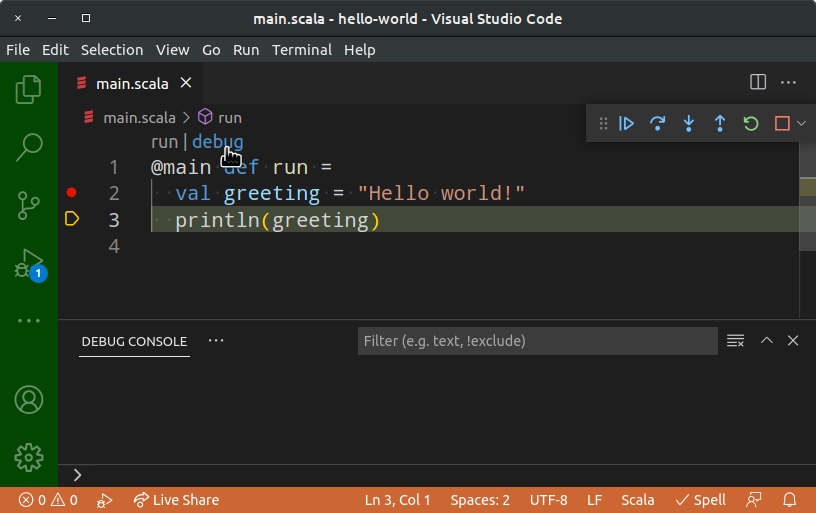
\includegraphics[width=\textwidth]{../img/vscode-debug.png}
% \end{Slide}
  

% \begin{Slide}{IntelliJ IDEA med Scala-plugin}
% 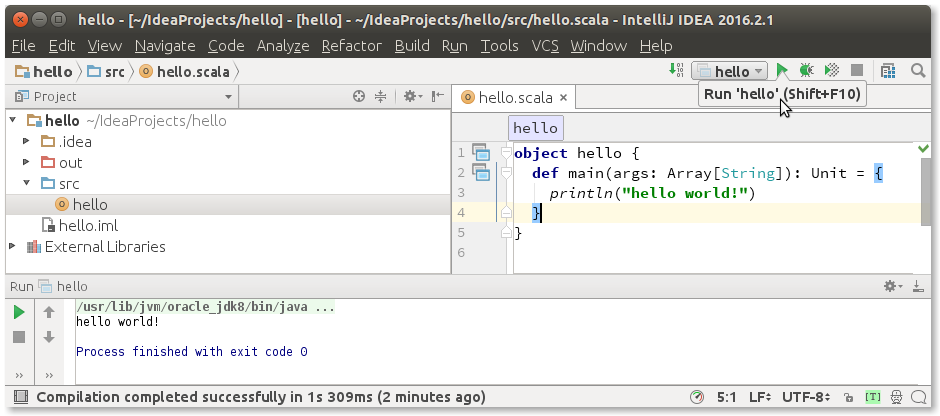
\includegraphics[width=\textwidth]{../img/intellij/idea-hello.png}
% \end{Slide}

% \begin{Slide}{Eclipse med ScalaIDE}
% 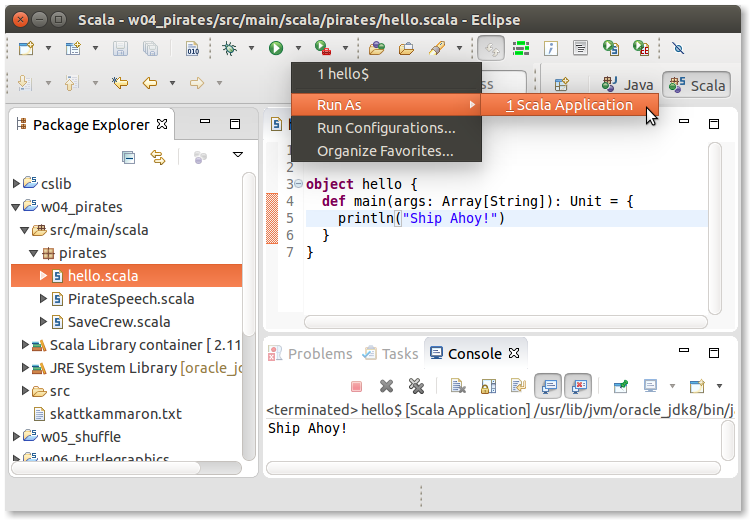
\includegraphics[width=\textwidth]{../img/eclipse/eclipse-pirates-hello.png}
% \end{Slide}



%!TEX encoding = UTF-8 Unicode

%!TEX root = ../compendium2.tex

\chapter{Arv, Gränssnitt}
\begin{itemize}[nosep]
\item klasser
\item arv
\item polymorfism
\item likhet
\item equals
\item accessregler
\item private
\item public
\item protected
\item private[this]
\item trait
\item inmixning
\item Any
\item AnyVal
\item AnyRef
\item Nothing\end{itemize}
\newpage

%!TEX encoding = UTF-8 Unicode

%!TEX root = ../compendium1.tex

\chapter{Sökning, Sortering}\label{chapter:W10}
\begin{itemize}[nosep]
\item algoritm: LINEAR-SEARCH
\item algortim: BINARY-SEARCH
\item algoritmisk komplexitet
\item sortering till ny vektor
\item sortering på plats
\item algoritm: INSERTION-SORT
\item algoritm: SELECTION-SORT
\end{itemize}
\clearpage
%!TEX encoding = UTF-8 Unicode
%!TEX root = ../lect-w10.tex

%%%


%\begin{Slide}{TODO: Begrepp att förklara}
%  Tänk igenom ordningen:
%  \begin{itemize}
%    \item java switch, scala match ... 
%  \end{itemize}
%\end{Slide}
%
%
%\begin{Slide}{Javas switch-sats}
%A switch in Java works with the byte, short, char, and int primitive data types. It also works with enumerated types (discussed in Enum Types), the String class, and a few special classes that wrap certain primitive types: Character, Byte, Short, and Integer
%\end{Slide}


\Subsection{Veckans lab: \texttt{chords-team}}
\begin{Slide}{Veckans lab: \texttt{chords-team}}\SlideFontSmall
Övergripande syfte:
\begin{itemize}
\item Träna på case-klasser, matchning, undantag
\item Jobba med ett större program med flera delar i olika filer
\item Jobba flera personer på samma program
\end{itemize}
Innehåll:
\begin{itemize}
\item Skapa och spara ackord på gitarr (6 strängar) och ukulele (4 strängar) 
\item Spela upp ackord med Javas inbyggda musikspelare inkapslad i \code{SimpleNotePlayer}
\item Rita ackord med \code{SimpleWindow} 
\end{itemize}
Hur mycket ni gör beror på hur många ni är i gruppen och hur stora ambitioner ni har. Diskutera detta med handledare på resurstid.
\end{Slide}

\begin{Slide}{Toner, oktaver och ackord}\SlideFontSmall
\begin{itemize}
\item Det finns 12 toner som har speciella namn: \\ C, C\#, D, D\#, etc. (uttalas: c, ciss, d, diss, etc.)
\item Jämför vita och svarta tangenter på ett piano: \\ avståndet mellan varje tangent är ett s.k. \emph{halvt tonsteg}. 
\item Toner återkommer i oktaver, modulo 12.
\item Tonen som representeras av strängen \code{"D2"} är tonen D i andra oktaven.
\item Tonen \code{"D2"} motsvarar heltalet \code{26} på labben.
\item Ett ackord består av flera toner.
\end{itemize}
\begin{REPL}[basicstyle=\color{white}\ttfamily\SlideFontSize{6}{7}\selectfont]
scala> val notes = Vector("C", "C#", "D", "D#", "E", "F", "F#", "G", "G#", "A", "A#", "B")

scala> notes.size
res0: Int = 12

scala> notes(26 % 12)
res1: String = D

\end{REPL}
\end{Slide}

\begin{Slide}{Toner på ett stränginstrument}
\begin{minipage}{0.5\textwidth}
\begin{itemize}\SlideFontSmall
\item Gitarr och ukulele har 6 resp. 4 strängar och en greppbräda med s.k. band.

\item Om man trycker ned ett finger på (egentligen bakom) första bandet höjs tonen ett halvt tonsteg. 

\item Exempel: om en sträng är stämd i D3 blir tonen om man trycker ned fingret på fjärde bandet F\#3.

\item \href{http://www.gitarr.org}{www.gitarr.org}

\item \href{http://www.stefansukulele.com}{www.stefansukulele.com}

\end{itemize}
\end{minipage}
\begin{minipage}{0.45\textwidth}
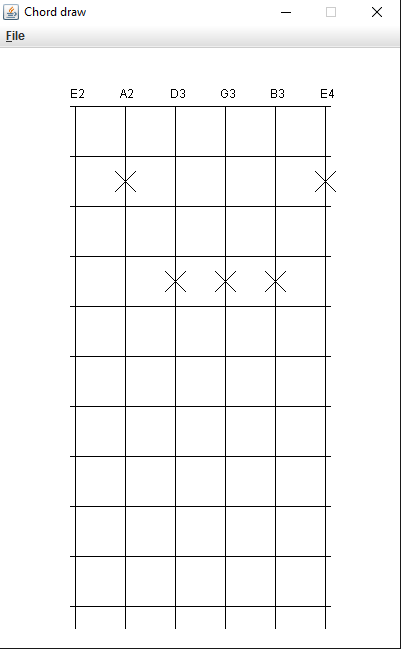
\includegraphics[width=1.0\textwidth]{../img/chords/ChordDraw}
\end{minipage}

\end{Slide}

\begin{Slide}{Modell av gitarr och ukulele}
\begin{Code}
object model {

  type Tuning = Vector[String]
  type Grip = Vector[Int]

  trait Chord {
    def name: String
    def tuning: Tuning
    def grip: Grip
  }
  
  case class Guitar(name: String, grip: Grip) extends Chord {
    val tuning = Vector("E2", "A2", "D3", "G3", "B3", "E4")
  }
  
  case class Ukulele(name: String, grip: Grip) extends Chord {
    val tuning = Vector("G4", "C4", "E4", "A4")
  }

}
\end{Code}
\end{Slide}

\begin{Slide}{En gemensam bastyp för olika ackord}\SlideFontSmall
\vspace{-0.5em}\begin{center}
\newcommand{\TextBox}[1]{\raisebox{0pt}[1em][0.5em]{#1}}
\tikzstyle{umlclass}=[rectangle, draw=black,  thick, anchor=north, text width=3cm, rectangle split, rectangle split parts = 3]
\begin{tikzpicture}[inner sep=0.5em]
\node [umlclass, rectangle split parts = 2, xshift=0cm, text width=5cm] (BaseType)  {
            \textit{\textbf{\centerline{\TextBox{\code{Chord}}}}}
            \nodepart[]{second}
            \TextBox{\code{def name: String}}\vspace{-0.25em}\newline
            \TextBox{\code{def tuning: Vector[String]}}\vspace{-0.25em}\newline
            \TextBox{\code{def grip: Vector[Int]}}\vspace{-0.25em}\newline

        };
        
\node [umlclass, rectangle split parts = 1]  at (2.5cm,-3.7cm) (SubType1) {
            \textbf{\centerline{\TextBox{\code{Guitar}}}}
            %\nodepart[]{second} \TextBox{~}
        };  
                
\node [umlclass, rectangle split parts = 1] at (-2.5cm,-3.7cm) (SubType2)  {
            \textbf{\centerline{\TextBox{\code{Ukulele}}}}
            %\nodepart[]{second} \TextBox{talk(): void}
        };        
\draw[umlarrow] (SubType1.north) -- ++(0,0.5) -| (BaseType.south);    
\draw[umlarrow] (SubType2.north) -- ++(0,0.5) -| (BaseType.south);            
\end{tikzpicture}
\end{center}
\pause\vspace{-0.7em}
\begin{REPL}
scala> import model._

scala> val uc = Ukulele("C", Vector(0, 0, 0, 3))
uc: model.Ukulele = Ukulele(C,Vector(0, 0, 0, 3))

scala> val ge = Guitar("E", Vector(0, 2, 2, 1, 0, 0))
ge: model.Guitar = Guitar(E,Vector(0, 2, 2, 1, 0, 0))
\end{REPL}
\end{Slide}


\begin{Slide}{Grupparbete}\SlideFontSmall
\begin{itemize}
\item Förslag på arbetssätt:
\begin{itemize}\SlideFontSmall
\item Träffas nu på rasten och boka nästa gruppmöte
\item Förberedelser inför första gruppmötet: individuella studier av labbinstruktioner och koden som är given i workspace \\
\href{https://github.com/lunduniversity/introprog/tree/master/workspace/w08_chords_team/src}{.../workspace/w08\_chords\_team/src} \\
OBS! numrering av labbarna enl. ''gamla'' veckor
\item Träffas gärna i ett studierum med whiteboard
\item På mötet: gå igenom uppgift och given kod så att alla fattar vad det går ut på; bestäm omfattning och ansvarsuppdelning
\item När ni träffas, skissa upp den kod som just du håller på med på whiteboard och få feedback och ge feedback till andra
\item På varje gruppmöte, bestäm tid för nästa möte och vad var och en ska försöka hinna tills dess
\end{itemize}


\item Ni får \Emph{lov att ändra på omfattningen} efter antalet gruppmedlemmar, ambition och förmåga: diskutera detta med handledare på resurstid

\item \Alert{Minimikrav}: att med textkommando kunna skapa/spara/ladda gitarr- och ukulele-ackord och att ni tränar på matchning

\end{itemize}
\end{Slide}


\Subsection{Matchning}

\begin{Slide}{Vad är matchning?}
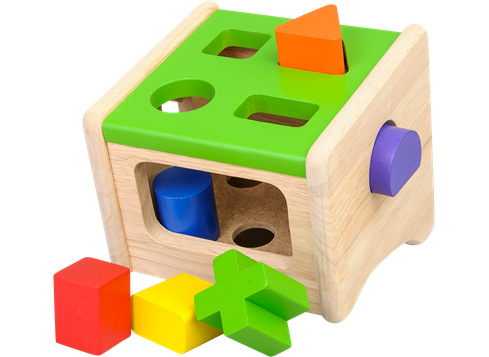
\includegraphics[width=0.8\textwidth]{../img/plocklada.png}
\end{Slide}


\begin{Slide}{Vad är matchning?}
Matchning gör man då man vill jämföra ett värde mot andra värden och hitta överensstämmelse \Eng{match}.

\pause

\vspace{1em}Detta kan man t.ex. göra med nästlade if-else-satser/uttryck:

\begin{Code}
val g = scala.io.StdIn.readLine("grönsak:")
val smak = 
  if (g == "gurka") "gott!"
  else if (g == "tomat") "jättegott!"
  else if (g == "broccoli") "ganska gott..."
  else "inte gott :("

println(g + " är " + smak)
\end{Code}
\end{Slide}




\begin{Slide}{Javas switch-sats}\SlideFontSmall
De flesta C-liknande språk (men inte Scala) har en \jcode{switch}-sats som man kan använda istället för (vissa) nästlade if-else-satser: 
\javainputlisting[basicstyle=\ttfamily\SlideFontSize{5.5}{6.8}\selectfont]{../compendium/examples/match/Switch.java}

\vspace{-0.5em}Funkar bara för primitiva typer och några till (t.ex. String).
\end{Slide}




\begin{Slide}{Javas switch-sats utan break}\SlideFontSmall
Saknad \jcode{break}-sats ''faller igenom'' till efterföljande gren: 

\javainputlisting[basicstyle=\ttfamily\SlideFontSize{6}{7}\selectfont]{../compendium/examples/match/SwitchNoBreak.java}
En glömd \jcode{break} kan ge svårhittad bugg... 
\end{Slide}

\begin{Slide}{Javas switch-sats med glömd break}\SlideFontSmall

\vspace{-0.5em}\javainputlisting[basicstyle=\ttfamily\SlideFontSize{5.5}{6.8}\selectfont]{../compendium/examples/match/SwitchForgotBreak.java}

\vspace{-0.7em}\pause
\begin{REPL}
$ java SwitchForgotBreak 
Skriv grönsak:
gurka
gott!
gott!
\end{REPL}

\end{Slide}


\begin{Slide}{Scalas \texttt{match}-uttryck}\SlideFontSmall
Scala har ingen \code{switch}-sats men erbjuder i stället ett \code{match}-\Emph{uttryck} som är kraftfullare och ger ett värde.

\begin{Code}
val g = scala.io.StdIn.readLine("grönsak:")
val smak = g match {
  case "gurka" => "gott!"
  case "tomat" => "jättegott!"
  case "broccoli" => "ganska gott..."
  case _ => "mindre gott..."
}
println(g + " är " + smak)
\end{Code}
Och den ''faller inte igenom'' som Javas \code{switch}-sats! 
\begin{itemize}
\pause\item Varje \code{case}-gren testas var för sig i tur och ordning uppifrån och ned.
\pause\item Det som står mellan \code{case} och \code{=>} kallas ett \Emph{mönster} \Eng{pattern}
\pause\item Sista default-grenen ovan kallas \Emph{wildcard-mönster}: \code{case _ => } 
\pause\item Ovan är exempel på matchning mot \Emph{konstant-mönster}, \\ i detta fallet tre stycken strängkonstantmönster.
\pause\item Det finns många andra sätt att skriva mönster.
\end{itemize}
\end{Slide}



\begin{Slide}{Matchning med gard}
Man kan stoppa in en s.k \Emph{gard} \Eng{guard} innan pilen \code{=>} för att villkora matchningen: (notera \code{if}, parenteser behövs ej)
\begin{Code}
val g = scala.io.StdIn.readLine("grönsak:")
def f = g match {
  case "gurka" if math.random > 0.5 => "gott ibland!"
  case "tomat" => "jättegott!"
  case "broccoli" => "ganska gott..."
  case _ => "mindre gott..."
}
\end{Code}
\code{case}-grenen med gard ger bara en lyckad matchning \\ om uttrycket efter \code{if} är sant; annars provas nästa gren, etc.
\end{Slide}

\begin{Slide}{Matchning med variabelmönster}\SlideFontSmall
Om det finns ett namn efter \code{case} som börjar med liten begynnelsebokstav, blir detta namn en variabel som automatiskt binds till uttrycket före \code{match}:

\begin{Code}
val g = scala.io.StdIn.readLine("grönsak:")
def f = g match {
  case "gurka" if math.random > 0.5 => "gott ibland!"
  case "tomat" => "jättegott!"
  case "broccoli" => "ganska gott..."
  case other => "smakar bakvänt: " + other.reverse
}
\end{Code}

Ett enkelt variabelmönster, så som \\ \code{case other => ...} \\ i exemplet ovan, matchar \Emph{allt}! \\\code{other} får alltså värdet av \code{g} om \code{g} \Alert{inte} är \code{"gurka"}, \code{"tomat"}, \code{"broccoli"}.  

\end{Slide}





\begin{Slide}{Matchning med typade mönster}\SlideFontSmall
Med en typannotering efter en variabel får man ett \Emph{typat mönster} \Eng{typed pattern}. Om matchningen lyckas blir värdet \Alert{omvandlat} till den specifika typen och binds till variabeln.
\begin{Code}
def f = if (math.random < 0.5) 42 + math.random else "gurka" + math.random
def g = f match {
  case x: Double => x.round.toInt
  case s: String => s.length
}
\end{Code}
Vad har funktionen \code{f} för returtyp? \\ \pause
Matchning mot specifika typer enl. ovan används i idiomatisk Scala hellre än \code{isInstanceOf} men man kan göra motsvarande ovan med if-uttryck:
\begin{Code}
def g2 = {
  val x = f
  if (x.isInstanceOf[Double]) x.asInstanceOf[Double].round.toInt
  else if (x.isInstanceOf[String]) x.asInstanceOf[String].length
}.asInstanceOf[Int]
\end{Code}
\end{Slide}


\begin{Slide}{Konstruktormönster med case-klasser}\SlideFontSmall
En basklass med gemensamma delar och två subtyper:
\begin{Code}
trait Grönsak {
  def vikt: Int
  def ärRutten: Boolean
}
case class Gurka(vikt: Int, ärRutten: Boolean) extends Grönsak
case class Tomat(vikt: Int, ärRutten: Boolean) extends Grönsak
\end{Code}
\pause
Tack vare case-klasserna kan man använda \Emph{konstruktormönster} \Eng{constructor pattern} för att kolla vad som finns \Alert{inuti} en instans:
\begin{Code}
def testa(g: Grönsak): String = g match {
  case Gurka(v, false) => "gott, väger " + v
  case Gurka(_, true)  => "inte gott"
  case Tomat(v, r)     => (if (r) "inte " else "") + "gott, väger " + v 
  case _ => "okänd grönsak: " + g
}
\end{Code}

Konstruktormönster ''\Emph{plockar isär}'' det som matchas och binder variabler till de attribut som finns i case-klassens konstruktor.
\end{Slide}


\begin{Slide}{Plocka isär samlingar med djupa mönster}
Man kan plocka isär innehållet i en samling så här:
\begin{Code}
def visa(xs: Vector[Grönsak]): String = xs match {
  case Vector()               => "tom grönsaksvektor"
  case Vector(Gurka(v, true)) => "en rutten gurka som väger " + v
  case Vector(g)              => "exakt en grönsak: " + g
  case Vector(g1, g2)         => s"exakt två grönsaker: $g1, $g2"
  case g +: gs                => s"först en $g och sedan svansen: $gs" 
}
\end{Code}
Övning: prova ovan i REPL. Vad händer om du byter ordning på andra och tredje mönstret ovan?
\end{Slide}

\begin{Slide}{Mönstermatchning och case-objekt}
En bastyp och specifika singelobjekt av gemensam typ:
\begin{Code}
trait Färg
case object Spader  extends Färg
case object Hjärter extends Färg
case object Ruter   extends Färg
case object Klöver  extends Färg

def parallellFärg(f: Färg): Färg = f match {
  case Spader  => Klöver
  case Klöver  => Spader
  case Hjärter => Ruter
}
\end{Code}
Vilken case-gren har vi glömt? Kan kompilatorn hjälpa oss?
\pause
\begin{REPL}
scala> parallellFärg(Ruter)
scala.MatchError: Ruter (of class Ruter$)
  at .parallellFärg(<console>:18)

\end{REPL}
Runtime exception \code{:(} ~~och en bugg som kan vara svårhittad...
\end{Slide}

\begin{Slide}{Mönstermatchning och förseglade typer}
Med nyckelordet \code{sealed} får vi en kompileringsvarning \code{:)}
\begin{Code}
sealed trait Färg
case object Spader  extends Färg
case object Hjärter extends Färg
case object Ruter   extends Färg
case object Klöver  extends Färg

def parallellFärg(f: Färg): Färg = f match {
  case Spader  => Klöver
  case Klöver  => Spader
  case Hjärter => Ruter
}
\end{Code}
\begin{REPL}
// Exiting paste mode, now interpreting.

<console>:23: warning: match may not be exhaustive.
It would fail on the following input: Ruter
       def parallellFärg(f: Färg): Färg = f match {
\end{REPL}
\end{Slide}

\begin{Slide}{Stora/små begynnelsebokstäver vid matchning}
Fallgrop: att försöka matcha på värdet av en variabel som börjar med liten bokstav.
\begin{REPL}
scala> val livetsMening = 42

scala> def ärLivetsMeningBuggig(svar: Int) = svar match {
         case livetsMening => true    // lokalt namn som matchar allt!
         case _ => false
       }

scala> ärLivetsMeningBuggig(43)
res0: Boolean = true

scala> val LivetsMening = 42   // stor begynnelsebokstav

scala> def ärLivetsMening(svar: Int) = svar match {
         case LivetsMening => true    // funkar fint!
         case _ => false
       }

scala> ärLivetsMening(43)
res1: Boolean = false
\end{REPL}
\end{Slide}


\begin{Slide}{Stora/små begynnelsebokstäver vid matchning}
Ett sätt att komma runt problemet med liten begynnelsebokstav: \\
\Emph{backticks} to the rescue!
\begin{REPL}
scala> val livetsMening = 42

scala> def ärLivetsMeningBackTicks(svar: Int) = svar match {
         case `livetsMening` => true    // nu funkar det!
         case _ => false
       }

scala> ärLivetsMeningBackTicks(43)
res2: Boolean = false
\end{REPL}
\end{Slide}


\begin{Slide}{Mönster på andra ställen än i \texttt{match}}\SlideFontSmall
Mönster i \Emph{deklarationer}:
\vspace{-0.25em}\begin{REPL}
scala> case class Point(x: Int, y: Int)

scala> val p = Point(0, 1)

scala> val Point(x, y) = p          // konstruktormönster med case-klass
x: ???
y: ???

scala> val (x, y, z) = (0, 1, 2)    // konstruktormönster med tupel
x: ???
y: ???
z: ???

\end{REPL}
Mönster i \Emph{for-satser}:
\vspace{-0.25em}\begin{REPL}
scala> val xs = for ((x, y) <- Vector((1,2), (3,4))) yield x
xs: ???
\end{REPL}

\end{Slide}

\begin{Slide}{Mönster på andra ställen än i \texttt{match}}\SlideFontSmall
Mönster i \Emph{deklarationer}:
\vspace{-0.25em}\begin{REPL}
scala> case class Point(x: Int, y: Int)

scala> val p = Point(0, 1)

scala> val Point(x, y) = p          // konstruktormönster med case-klass
x: Int = 0
y: Int = 1

scala> val (x, y, z) = (0, 1, 2)    // konstruktormönster med tupel
x: Int = 0
y: Int = 1
z: Int = 2

\end{REPL}
Mönster i \Emph{for-satser}:
\vspace{-0.25em}\begin{REPL}
scala> val xs = for ((x, y) <- Vector((1,2), (3,4))) yield x
xs: scala.collection.immutable.Vector[Int] = Vector(1, 3)
\end{REPL}
\end{Slide}

\begin{Slide}{Fördjupning om mönster}
Avancerade saker för den intresserade (ingår ej): 
\begin{itemize}
\item binda variabler till mönsterdelar med \code{@}
\item partiella funktioner
\item att skapa extraherare med \code{unapply} och \code{unapplySeq}
\end{itemize}
Fördjupning:
\begin{itemize}
\item Läs mer om mönster här:  \href{http://www.artima.com/pins1ed/case-classes-and-pattern-matching.html}{\SlideFontTiny www.artima.com/pins1ed/case-classes-and-pattern-matching.html}

\item För djupare förståelse av hur \code{case} fungerar, läs speciellt om \Emph{partiella funktioner} här: \href{http://www.artima.com/pins1ed/case-classes-and-pattern-matching.html\#15.7}{\SlideFontTiny www.artima.com/pins1ed/case-classes-and-pattern-matching.html\#15.7}

\item Läs om extractors här: \href{http://www.artima.com/pins1ed/extractors.html}{\SlideFontTiny www.artima.com/pins1ed/extractors.html}

\end{itemize} 
\end{Slide}


\begin{Slide}{Fördjupning: metoden \texttt{unapply}}\SlideFontSmall
När du deklarerar en case-klass kommer kompilatorn att \Alert{automatiskt generera en metod} med namnet \Emph{\texttt{unapply}} som kan plocka isär instansen.
\begin{REPL}
scala> case class Gurka(vikt: Int, ärRutten: Boolean)

scala> Gurka.unapply // tryck TAB två gånger för att se metodhuvudet
 case def unapply(x$0: Gurka): Option[(Int, Boolean)]
 
scala> val g = Gurka(100, false)

scala> Gurka.unapply(g)
res0: Option[(Int, Boolean)] = Some((100,false))
\end{REPL}
Vi ska snart se hur \code{Option} kan hantera värden som \Emph{eventuellt} \Alert{saknas}. \\
\pause

{\SlideFontTiny\vspace{1em}\emph{Fördjupning:} Ett anrop av metoden \code{unapply} genereras av kompilatorn vid matchning och det är det som gör att case-klasser kan användas i konstruktormönster. Man kan skapa en egna s.k. extraktorer \Eng{extractors} som funkar i matchningar (se övn. 22).}
\end{Slide}







%!TEX encoding = UTF-8 Unicode
%!TEX root = ../lect-w10.tex

%%%

\Subsection{Option}


\begin{Slide}{Hur hantera saknade värden?}\SlideFontSmall
Olika sätt att hantera saknade värden:
\begin{itemize}
\item Hitta på ett specialvärde: exempel -1 för icke nedtryckt sträng
\item \code{null} om \code{AnyRef}/\code{Object} (vanligt i Java, mkt ovanligt i Scala) 
\item Använd en samling och låt tom samling representera saknat värde: \\
\code{val grip = Vector(Vector(2), Vector(7), Vector(), Vector(3))}

\item \code{Option[T]} gemensam bastyp för: \\
  \code{None} som representerar \Alert{saknat värde}, och \\ \code{Some[T]} som representerar att \Emph{värde finns}
\end{itemize}
\end{Slide}

\begin{Slide}{En gemensam bastyp för ett värde som kanske saknas}\SlideFontSmall
\vspace{-0.0em}\begin{center}
\newcommand{\TextBox}[1]{\raisebox{0pt}[1em][0.5em]{#1}}
\tikzstyle{umlclass}=[rectangle, draw=black,  thick, anchor=north, text width=3cm, rectangle split, rectangle split parts = 3]
\begin{tikzpicture}[inner sep=0.5em]
\node [umlclass, rectangle split parts = 2, xshift=0cm, text width=3.5cm] (BaseType)  {
            \textit{\textbf{\centerline{\TextBox{\code{Option[A]}}}}}
            \nodepart[]{second}
            \TextBox{\code{def get: A}}\newline
            \TextBox{\code{def isEmpty: Boolean}}

        };
        
\node [umlclass, rectangle split parts = 1]  at (-2.5cm,-3.0cm) (SubType1) {
            \textbf{\centerline{\TextBox{\code{Some[A]}}}}
            % \nodepart[]{second} \TextBox{\code{val x: A}}
        };  
                
\node [umlclass, rectangle split parts = 1] at (2.5cm,-3.0cm) (SubType2)  {
            \textbf{\centerline{\TextBox{\code{None}}}}
        };        
\draw[umlarrow] (SubType1.north) -- ++(0,0.5) -| (BaseType.south);    
\draw[umlarrow] (SubType2.north) -- ++(0,0.5) -| (BaseType.south);            
\end{tikzpicture}
\end{center}
\pause
\vspace{-0.5em}\begin{REPL}
scala> var x: Option[Int] = Some(42)

scala> x.isEmpty
res0: Boolean = false

scala> x = None

scala> x.isEmpty
res1: Boolean = true
\end{REPL}
\end{Slide}


\begin{Slide}{Option för hantering av ev. saknade värden}\SlideFontSmall
Alla vill inte berätta för Facebook vad de har för kön. \\ Förbättra Facebooks kod med ett litet Scala-program:
\begin{Code}
trait Gender
case object Male   extends Gender
case object Female extends Gender

case class Person(name: String, gender: Option[Gender])
\end{Code}
\pause
\begin{REPL}
scala> val p1 = Person("Björn",  Some(Male))
scala> val p2 = Person("Sandra", Some(Female))
scala> val p3 = Person("Andro",  None)
scala> val g2 = p2.gender
scala> def show(g: Option[Gender]): String = g match {
         case Some(x) => x.toString
         case None    => "unknown"
       }
scala> show(g2)
scala> show(p3.gender)
scala> val ps = Vector(p1,p2,p3)
scala> ps.map(_.gender).map(show)
\end{REPL}
\end{Slide}

\begin{Slide}{Några smidiga metoder på \code{Option}}\SlideFontSmall
Metoden \code{getOrElse} gör att man ofta kan undvika matchning.
\begin{Code}
var opt: Option[Int] = None

val x = opt.getOrElse(42)      // get the value or give a default if missing
\end{Code}

Flera av de vanliga samlingsmetoderna funkar, t.ex. \code{foreach} och \code{map}.
\begin{Code}
opt.foreach{x => println(x)}    // only done if value exists

opt.map{x => x + 1}             // only done if value exists

opt = Some(42)                  // change opt to now have some value

opt.foreach{x => println(x)}    // done as value now exists

opt.map{x => x + 1}             // done as value now exists

\end{Code}
\end{Slide}


\begin{Slide}{Några samlingsmetoder som ger en \code{Option}}
\begin{REPL}
scala> val (xs, ys) = (Vector(1,2,3), Vector())

scala> xs.headOption
res0: ???

scala> ys.headOption
res1: ???

scala> xs.find(_ > 1)
res2: ???

scala> xs.find(_ > 5)
res3: ???

scala> val huvudstad = Map("Sverige" -> "Sthlm", "Skåne" -> "Malmö")

scala> huvudstad.get("Skåne")
res4: ???

scala> huvudstad.get("Danmark")
res5: ???
\end{REPL}
\end{Slide}

\begin{Slide}{Några samlingsmetoder som ger en \code{Option}}
\begin{REPL}
scala> val (xs, ys) = (Vector(1,2,3), Vector())

scala> xs.headOption
res0: Option[Int] = Some(1)

scala> ys.headOption
res1: Option[Nothing] = None

scala> xs.find(_ > 1)
res2: Option[Int] = Some(2)

scala> xs.find(_ > 5)
res3: Option[Int] = None

scala> val huvudstad = Map("Sverige" -> "Sthlm", "Skåne" -> "Malmö")

scala> huvudstad.get("Skåne")
res4: Option[String] = Some(Malmö)

scala> huvudstad.get("Danmark")
res5: Option[String] = None
\end{REPL}
\end{Slide}





%!TEX encoding = UTF-8 Unicode
%!TEX root = ../lect-w10.tex

%%%



\Subsection{Undantag}
\begin{Slide}{Vad är ett undantag \Eng{exception}?}
Undantag representerar ett fel eller ett onormalt tillstånd som upptäcks under exekvering och som  behöver hanteras på särskilt sätt vid sidan av det normala exekveringsflödet. 

\vspace{1em}\href{https://sv.wikipedia.org/wiki/Undantagshantering}{sv.wikipedia.org/wiki/Undantagshantering}


\vspace{1em} Exempel på undantag:

\pause

\begin{itemize}
\item Indexering utanför vektorns indexgränser.

\item Läsning bortom filens slut.

\item Försök att öppna en fil som inte finns.

\item Minnet är slut.

\item Division med noll.

\item \code{"hej".toInt} resulterar i \\\code{java.lang.NumberFormatException}

\end{itemize}

\end{Slide}

\begin{Slide}{''Kasta'' dina egna undantag med \texttt{throw}}\SlideFontSmall
Man kan själv generera ett undantag med \code{throw}, vilket kallas att \Emph{kasta} ett undantag som (om det inte \Emph{fångas}), gör att exekveringen \Alert{avbryts}.


\begin{REPL}
scala> def pang = throw new Exception("PANG!")
pang: Nothing

scala> pang
java.lang.Exception: PANG!
  at .pang(<console>:11)
  ...
  
\end{REPL}
\pause
Olika sätt att hantera undantag: 
\begin{itemize}
\item Scala: Man kan använda ett \code{try ... catch}-uttryck och ge ett \Emph{värde} i händelse av undantag.
\item Java: Man kan använda en \code{try ... catch}-sats och \Alert{göra något} i händelse av undantag.
 
\item Scala: Man kan \Emph{kapsla in} ett undantag med \Emph{\texttt{scala.util.Try}} och förhindra att exekveringen avbryts. (Finns ej i Java; att föredra i Scala.)
\end{itemize}
\end{Slide}


\Subsection{\texttt{scala.util.Try}}

\begin{Slide}{En gemensam bastyp för något som kan misslyckas}\SlideFontSmall
\begin{Code}
import scala.util.{Try, Success, Failure}
\end{Code}

\vspace{-0.5em}\begin{center}
\newcommand{\TextBox}[1]{\raisebox{0pt}[1em][0.5em]{#1}}
\tikzstyle{umlclass}=[rectangle, draw=black,  thick, anchor=north, text width=3.0cm, rectangle split, rectangle split parts = 3]
\begin{tikzpicture}[inner sep=0.5em]
\node [umlclass, rectangle split parts = 2, xshift=0cm, text width=3.8cm] (BaseType)  {
            \textit{\textbf{\centerline{\TextBox{\code{Try[T]}}}}}
            \nodepart[]{second}
            \TextBox{\code{def get: T}}\newline
            \TextBox{\code{def isFailure: Boolean}}\newline
            \TextBox{\code{def isSuccess: Boolean}}
        };
        
\node [umlclass, rectangle split parts = 2, text width=2.2cm]  at (-2.5cm,-3.7cm) (SubType1) {
            \textbf{\centerline{\TextBox{\code{Success[T]}}}}
            \nodepart[]{second} \TextBox{\code{val value: T}}
        };  
                
\node [umlclass, rectangle split parts = 2, text width=4.2cm] at (2.5cm,-3.7cm) (SubType2)  {
            \textbf{\centerline{\TextBox{\code{Failure[T]}}}}
            \nodepart[]{second} \TextBox{\code{val exception: Throwable}}
        };        
\draw[umlarrow] (SubType1.north) -- ++(0,0.5) -| (BaseType.south);    
\draw[umlarrow] (SubType2.north) -- ++(0,0.5) -| (BaseType.south);            
\end{tikzpicture}
\end{center}
\end{Slide}

\begin{Slide}{Hantera undantag med \texttt{Try}}
\vspace{-0.5em}\begin{REPL}
scala> def pang = throw new Exception("PANG!")

scala> def kanskePang = if (math.random < 0.5) 42 else pang

scala> import scala.util.{Try, Success, Failure}

scala> def försök = Try { kanskePang }

scala> val xs = Vector.fill(15){försök}

scala> val trettonde = xs(13) match {
         case Success(value) => value
         case Failure(e) => println(e); -1
       }

scala> (xs(13).isSuccess, xs(13).isFailure)

scala> försök.foreach(println)

scala> försök.map(_ + 1)

scala> for (Success(x) <- xs) yield x
\end{REPL}
\end{Slide}

\begin{Slide}{Fördjupning: \texttt{try}-\texttt{catch}-uttryck}\SlideFontSmall
Man kan fånga undantag med ett \code{try ... catch}-uttryck:
\begin{Code}
def carola = try {
  if (math.random > 0.5) throw new Exception("stormvind")
  42
} catch { 
  case e: Exception =>
    println("Fångad av en " + e.getMessage)
    -1
}  
\end{Code}
\pause
\begin{REPL}
scala> Vector.fill(5)(carola)
Fångad av en stormvind
Fångad av en stormvind
Fångad av en stormvind
res0: scala.collection.immutable.Vector[Int] = Vector(-1, 42, 42, -1, -1)
\end{REPL}
\pause
\emph{Fördjupning:} \\ Gör övning 9-10 som visar hur man fångar undantag i Scala och Java. \\Mer om undantag i fortsättningskursen.
\end{Slide}







%!TEX encoding = UTF-8 Unicode
%!TEX root = ../lect-w10.tex

%%%

\Subsection{\texttt{equals}}
\begin{Slide}{Fördjupning: Implementera \texttt{equals} med \texttt{match}}
Det visar sig att \Emph{innehållslikhet} är \Alert{förvånansvärt komplicerat} att implementera, speciellt  i samband med arv.
\begin{itemize}
\item Det enklare fallet: Gör övningsuppgift \code{patterns:14} och implementera \code{equals} för innehållslikhet utan arv. \\ En bra träning på att använda \code{match}!

\item Svårare: Gör fördjupningsövning \code{matching:21--22} om du vill se hur en \emph{komplett} \code{equals} ska se ut som funkar i alla lägen.

\end{itemize}

Det ingår inte på tentan att själv kunna implementera en generellt fungerande \code{equals}. Men du ska förstå skillnaden mellan referenslikhet och innehållslikhet. Mer om \code{equals} i fortsättningkursen, men en liten inblick i problemet nu...
\end{Slide}

\begin{Slide}{Fördjupning: \texttt{equals} som fungerar för finala klasser}
Recept för implementation av \code{equals} som fungerar för typer som \Alert{inte} har några subtyper:
\begin{Code}
final class Gurka(val vikt: Int, ärÄtbar: Boolean) {
  override def equals(other: Any): Boolean = other match {
    case that: Gurka => vikt == that.vikt && ärÄtbar == that.ärÄtbar
    case _ => false
  }
  override def hashCode: Int = (vikt, ärÄtbar).## // ger bra hashcode
}
\end{Code}
\begin{itemize}\SlideFontSmall
  \item
  Du \Alert{måste} alltid överskugga \code{hashCode} också om du överskuggar \code{equals} annars funkar inte gurksamlingar (lång story ...)
  \item
  Notera typen \code{Any} -- detta följer hur man valde att göra i Java (tyvärr?).
  \pause
  \item
  Ett \Alert{typsäkrare} innehållslikhetstest som \Emph{garanterat} bara jämför en gurka med en gurka och inget annat:
  \begin{Code}
    def ===(other: Gurka): Boolean =
      vikt == other.vikt && ärÄtbar == other.ärÄtbar
  \end{Code}
\end{itemize}
\end{Slide}


\begin{Slide}{Fördjupning: Recept i 8 steg för arvssäker \code{equals}}\SlideFontTiny
%fungerar även för klasser som inte är \code{final}:
\setlength{\leftmargini}{0pt}
\begin{enumerate}\SlideFontTiny
\item Inför denna metod: \code{ def canEqual(other: Any): Boolean}\\Observera att typen på parametern ska vara \code{Any}. Om subklass behövs \code{override}.

\item Metoden \code{canEqual} ska ge \code{true} om \code{other} är av samma typ som \code{this}, t.ex.: \code{override def canEqual(other: Any): Boolean = other.isInstanceOf[Gurka]}

\item Inför metoden \code{equals} och var noga med att parametern har typen \code{Any}: \\ \code{override def equals(other: Any): Boolean}

\item Implementera metoden \code{equals} med ett match-uttryck som börjar så här:
\code|other match { ... } |

\item Match-uttrycket ska ha två grenar. Den första grenen ska ha ett typat mönster för den klass som ska jämföras, t.ex.: \\ \code{  case that: Gurka =>}

\item Om du implementerar \code{equals} i den klass som inför \code{canEqual}, börja med: \\ \code{(that canEqual this) &&} \\
och skapa därefter en fortsättning som baseras på innehållet i klassen, t.ex.: \code{this.vikt == that.vikt && this.längd == that.längd} \\
Om du överskuggar equals vill du nog börja med
 \code{super.equals(that) && }

\item Den andra grenen i matchningen ska vara:
\code{case _ => false}

\item Överskugga \code{hashCode}, t.ex. med tupel av attributvärden och metoden \code{##}: \\
\code{override def hashCode: Int  = (vikt, längd).## }

\end{enumerate}
\url{http://www.artima.com/pins1ed/object-equality.html}

\end{Slide}

%!TEX encoding = UTF-8 Unicode

%!TEX root = ../compendium1.tex

%!TEX encoding = UTF-8 Unicode
\chapter{Scala och Java}\label{chapter:W11}
Koncept du ska lära dig denna vecka:
\begin{multicols}{2}\begin{itemize}[nosep,label={$\square$},leftmargin=*]
\item skillnader mellan Scala och Java
\item klasser i Scala vs Java
\item referensvariabler vs enkla värden i Java
\item referenstilldelning vs värdetilldelning i Java
\item alternativ konstruktor i Scala och Java
\item for-sats i Java
\item java for-each i Java
\item java.util.ArrayList
\item autoboxing i Java
\item primitiva typer i Java
\item wrapperklasser i Java
\item samlingar i Java vs Scala
\item scala.collection.JavaConverters
\item översiktligt om relationen mellan trait och interface
\item namnkonventioner för konstanter
\item enum i java ???\end{itemize}\end{multicols}


%!TEX encoding = UTF-8 Unicode

%!TEX root = ../compendium1.tex

\chapter{Trådar, Web, Android}
\begin{itemize}[nosep]
\item Thread
\item Future
\item HTML
\item Javascript
\item css
\item Scala.js
\item Android
\end{itemize}
\clearpage
%!TEX encoding = UTF-8 Unicode
%!TEX root = ../lect-week11.tex

%%%

\ifkompendium\else

\Subsection{Veckans labb: \texttt{survey2}}
\begin{Slide}{Veckans labb: \texttt{survey2}}\SlideFontTiny
\begin{minipage}{0.65\textwidth}
Nya version 2 av labben är enklare och kräver ej att du implementerar parsning av \code{args}. Välj själv vilken du gör.

\vspace{0.5em}
\Emph{Förberedelse:}
\begin{itemize}
\item Studera givna koden: {\SlideFontTiny \href{https://github.com/lunduniversity/introprog/tree/master/workspace/w10_survey2/src/main/scala/stats}{workspace/w10\_survey2}}
\item Fyll i denna enkät:
\\{\SlideFontTiny \url{https://goo.gl/forms/hC6JK2UQXVpbGECc2}} 
\end{itemize}

\Emph{Grunduppgift:}
\begin{itemize}
\item Implementera en klass \code{Table} för hantering av strängmatriser med rubrikrad från kolumnsepararade textfiler.
\item Öva på att kombinera matriser, sortering, registrering för att räkna statistik.
\item Använda inbyggda sorteringsfunktioner: \\\code{sortBy} och \code{sortWith}
\item Implementera din egen sortering ''från scratch''.
\end{itemize}
\Emph{Extrauppgift:}
\begin{itemize}
\item Implementera stapeldiagram.
\end{itemize}
\end{minipage}
\hfill\begin{minipage}{0.27\textwidth}
\centering
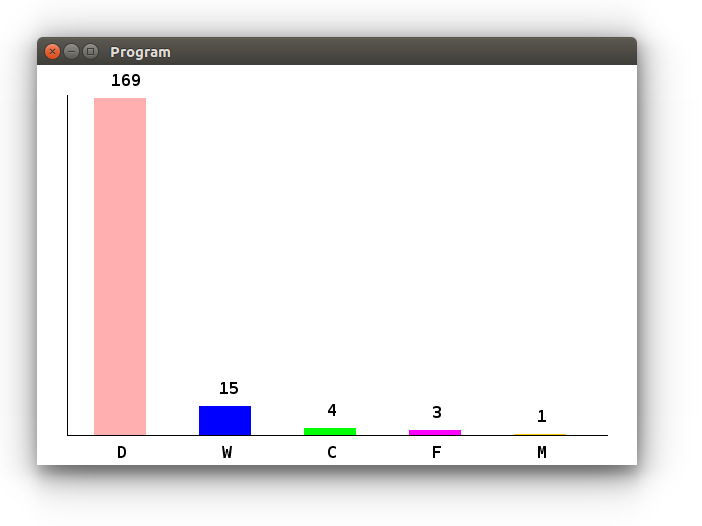
\includegraphics[width=0.9\textwidth]{../img/survey/bar}

\vspace{2em}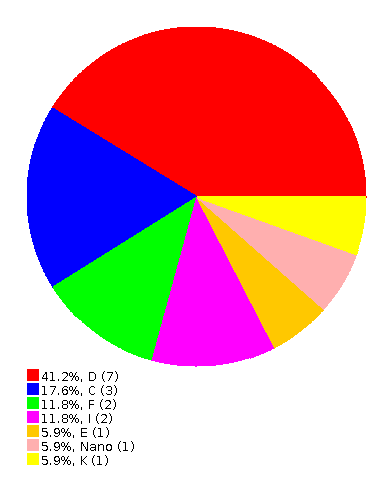
\includegraphics[width=0.7\textwidth]{../img/survey/pie}
\end{minipage}
\end{Slide}


\fi












%!TEX encoding = UTF-8 Unicode
%!TEX root = ../lect-w12.tex

%%%


\Subsection{Repetition: Vad är en algoritm?}
\begin{Slide}{Repetition: Vad är en algoritm? }\SlideFontTiny
\pause En \href{https://sv.wikipedia.org/wiki/Algoritm}{algoritm} är en stegvis beskrivning av hur man löser ett problem. \\ 
Exempel: SWAP, MIN, Registrering, Sökning, Sortering \\
\pause\vspace{0.5em}
Problemlösningsprocessens olika steg (inte nödvändigtvis i denna ordning): 
\begin{itemize}
\item Dela upp problemet i enklare delproblem och sätt samman.
\item Finns redan färdig lösning på (del)problem?
\item Formulera (del)\Emph{problemet} och ange tydligt indata och utdata: \\ exempel MIN: indata: sekvens av heltal; utdata: minsta talet
\item Kom på en \Emph{lösningsidé}: (kan  vara mycket klurigt och svårt) \\ exempel MIN: iterera över talen och håll reda på ''minst hittills''
\item Formulera en \Emph{stegvis beskrivning} som löser problemet: \\ exempel: pseudo-kod med sekvens av instruktioner
\item Implementera en \Emph{körbar lösning} i ''riktig'' kod: \\ exempel: en Scala-metod i en klass eller i ett singelobjekt
\item Har algoritmen acceptabel komplexitet i förhållande till tids- och minneskrav?
\end{itemize}
\pause Det krävs ofta \Emph{kreativitiet} i stegen ovan  -- även i att \Emph{känna igen} problemet!\\
Simpelt exempel: Du stöter på problemet MAX och ser likheten med MIN.\\
\pause\vspace{0.5em}\Emph{Övning}: Diskutera hur du löser detta problem i relation till stegen ovan: \\
\emph{Att räkna antalet förekomster av olika unika ord i en textsträng.} 
\end{Slide}













%!TEX encoding = UTF-8 Unicode
%!TEX root = ../lect-week11.tex

%%%

\ifkompendium\else

\Subsection{Jämföra strängar}

\begin{Slide}{Att jämföra strängar lexikografiskt}\SlideFontSmall
Teckenstandard \href{https://sv.wikipedia.org/wiki/UTF-16}{UTF-16}: Alla stora bokstäver är ''mindre'' än alla små:
\begin{REPLnonum}
scala> Array("hej","Hej","gurka").sorted
\end{REPLnonum}
\pause\vspace{-1.2em}
\begin{REPLnonum}
res0: Array[String] = Array(Hej, gurka, hej)\end{REPLnonum}
\pause
\begin{itemize}
\item Antag att vi vill lösa detta problem ''från scratch'': \\ \Emph{att sortera en sekvens med strängar} 
\item För att göra detta behöver vi lösa dessa delproblemen: 
\begin{itemize}
\item \Emph{att} \Alert{jämföra strängar}
\item \Emph{sökning i sekvenser}
\item \Emph{SWAP} (om på-plats-sortering i förändringsbar sekvens)
\end{itemize}
\item Vad betyder det att två strängar är ''lika''?

\item Vad betyder det att en sträng är ''mindre'' än en annan?
\end{itemize}
\pause {\SlideFontTiny Vi använder här strängjämförelse, sökning och sortering för att illustrera typiska \Emph{imperativa algoritmer}. \Alert{Normalt} använder man \Emph{färdiga lösningar} på dessa problem!}

\end{Slide}

\begin{Slide}{Jämföra strängar: likhet}\SlideFontSmall
Antag att vi inte kan göra \code{s1 == s2} utan bara kan jämföra strängar tecken för tecken, 
t.ex. så här: \code{s1(i) == s2(i)}. Antag också att vi inte har tillgång till annat än metoderna \code{length} och \code{apply} på strängar, samt  \code{while} och variabler av grundtyp. \Emph{Lös problemet att \emph{avgöra om två strängar är lika}.}

\pause
\begin{itemize}
\item Indata: två strängar
\item Utdata: \code{true} om lika annars \code{false}
\end{itemize}
\begin{enumerate}
\item Klura ut din lösningsidé
\item Formulera algoritmen i pseudokod
\item Implementera algoritmen i Scala: \code{def isEqual(s1: String, s2: String): Boolean} = ???
\end{enumerate}
\end{Slide}

\begin{Slide}{Algoritmexempel: stränglikhet, pseudokod}
\begin{Code}
def isEqual(s1: String, s2: String): Boolean = {
  if (/* lika längder */) {
    var foundDiff = false
    var i = /* första index */
    while (!foundDiff && /* i inom indexgräns */) {
      if (/* tecken på plats i är olika */) foundDiff = true
      else i = /* nästa index */
    }
    !foundDiff
  } else false
}
\end{Code}

\pause Detta är en variant av s.k. \Emph{linjärsökning} där vi söker från början i en sekvens till vi hittar det vi söker efter (här söker vi efter tecken som skiljer sig åt). 
\\\pause\vspace{2.5em} Hur ser implementationen i exekverbar Scala ut?
\end{Slide}

\begin{Slide}{Algoritmexempel: stränglikhet, implementation}\SlideFontSmall
\begin{Code}
def isEqual(s1: String, s2: String): Boolean = {
  if (s1.length == s2.length) {
    var foundDiff = false
    var i = 0
    while (!foundDiff && i < s1.length) {
      if (s1(i) != s2(i)) foundDiff = true
      else i += 1
    }
    !foundDiff
  } else false
}
\end{Code}
\pause 
{\SlideFontTiny Fördjupning: jämför ovan med implementationen av \code{String.equals} här:
\href{http://hg.openjdk.java.net/jdk8u/jdk8u60/jdk/file/935758609767/src/share/classes/java/lang/String.java#l976}{hg.openjdk.java.net/jdk8u/jdk8u60/jdk/file/935758609767/src/share/classes/java} \\ och använd \code{timed} nedan och jämför prestanda med \code{isEqual} ovan.\\
Obs! Mät många gånger så att JVM:en optimerar din kod.}
\vspace{-0.25em}\begin{Code}
def timed[T](block: => T): (Double, T) = { 
  val (t, res) = (System.nanoTime, block)
  ((System.nanoTime - t) / 1e9, res) 
}
\end{Code}

\end{Slide}

\begin{Slide}{Algoritmexempel: stränglikhet, prestanda}
\begin{REPL}
scala> val enMiljon = 1000000

scala> val s = Array.fill(enMiljon)('x').mkString

scala> val t = s.updated(enMiljon - 1, 'y')

scala> timed { s == t }
res42: (Double, Boolean) = (3.76459E-4,false)

scala> timed { isEqual(s,t) } 
res43: (Double, Boolean) = (3.31597E-4,false)
\end{REPL}
Ovan är kört efter ''uppvärmning'' på i7-4790K CPU @ 4.00GHz \\
Skillnaden inom mätfelmarginalen!
\end{Slide}



\begin{Slide}{Jämföra strängar: ''mindre än''}\SlideFontSmall
Med \code{s1 < s2} menar vi att strängen s1 ska sorteras före strängen s2 enligt hur de enskilda tecknen är ordnade med uttrycket \code{s1(i) < s2(i)}. \\
Antag också att vi inte har tillgång till annat än metoderna \code{length} och \code{apply} på strängar, samt  \code{while} och variabler av grundtyp, samt \code{math.min}
\\\Emph{Lös problemet att \emph{avgöra om en sträng är ''mindre'' än en annan}.}\\
\begin{itemize}
\item Indata: två strängar, s1, s2
\item Utdata: \code{true} om s1 ska sorteras före s2 annars \code{false}
\end{itemize}
\begin{enumerate}
\item Klura ut din lösningsidé
\item Formulera algoritmen i pseudokod
\item Implementera algoritmen i Scala: \code{def isLessThan(s1: String, s2: String): Boolean} = ???
\end{enumerate}
\end{Slide}

\begin{Slide}{Jämföra strängar: ''mindre än''}\SlideFontSmall
Pseudokod:
\begin{Code}
def isLessThan(s1: String, s2: String): Boolean = {
  
  val minLength = /* minimum av längderna på s1 och s2 */
  
  def firstDiff(s1: String, s2: String): Int = 
    /* index för första skillnaden (om de börjar lika: minLength) */

  val diffIndex = firstDiff(s1, s2)
  if (diffIndex == minLength) /* s1 är kortare än s2 */
  else /* tecknet s1(diffIndex) är mindre än tecknet s2(diffIndex) */ 
}
\end{Code}
\end{Slide}

\begin{Slide}{Jämföra strängar: ''mindre än''}\SlideFontSmall
\begin{Code}
def isLessThan(s1: String, s2: String): Boolean = {

  val minLength = math.min(s1.length, s2.length)

  def firstDiff(s1: String, s2: String): Int = {
    var foundDiff = false
    var i = 0
    while (!foundDiff && i < minLength) 
      if (s1(i) != s2(i)) foundDiff = true 
      else i += 1
    i
  }

  val diffIndex = firstDiff(s1, s2)
  if (diffIndex == minLength) s1.length < s2.length
  else s1(diffIndex) < s2(diffIndex)
}
\end{Code}
\end{Slide}

\begin{Slide}{Jämföra strängar i Java}\SlideFontTiny
\begin{itemize}
\item I Java kan man \Alert{inte} jämföra strängar med operatorerna \code{<}, \code{<=}, \code{>}, och \code{>=}

\item Dessutom ger operatorerna \code{==} och \code{!=} \emph{inte} innehålls(o)likhet utan \Alert{referens(o)likhet} \code{:(}

\item Istället \Alert{måste} man i Java använda metoderna \code{equals} och \code{compareTo} 
\\Dessa fungerar även i Scala eftersom strängar i Scala och Java är av samma typ, nämligen \code{java.lang.String}.
\pause
\item \code{s1.compareTo(s2)} ger ett heltal som är:
\begin{itemize}\SlideFontTiny
\item \code{0} om s1 och s2 har samma innehåll
\item \Alert{negativt} om s1 < s2 i lexikografisk mening, alltså s1 ska sorteras \Alert{före}
\item \Emph{positivt} om s1 > s2 i lexikografisk mening, alltså s1 ska sorteras \Emph{efter}
\end{itemize}

\pause
\item Undersök följande:
\begin{REPL}
scala> new String("hej") eq new String("hej") // motsvarar == i Java
scala> "hej".equals("hej")                    // samma som == i Scala
scala> "hej".compareTo("hej")
scala> "hej".compareTo("HEJ")         // alla stora är 'före' alla små
scala> "HEJ".compareTo("hej")
\end{REPL}
\end{itemize}

\href{http://docs.oracle.com/javase/8/docs/api/java/lang/String.html#compareTo-java.lang.String-}{docs.oracle.com/javase/8/docs/api/java/lang/String.html\#compareTo-java.lang.String-}
\end{Slide}


\begin{Slide}{Jämföra strängar i Java: exempel}\SlideFontSmall
Vad skriver detta Java-program ut?
\javainputlisting{../compendium/examples/StringEqTest.java}
\pause
\begin{REPL}
$ javac StringEqTest.java 
$ java StringEqTest 
false
true
0
\end{REPL}
\end{Slide}


\fi












%!TEX encoding = UTF-8 Unicode
%!TEX root = ../lect-week11.tex

%%%

\ifkompendium\else

\Subsection{Jämförelse Scala och Java}
\begin{Slide}{Grundläggande likheter och skillnader}\SlideFontSmall

\begin{itemize}
\item \Emph{Sökning} återkommer i många skepnader: \\ i en datastruktur, vilken det än må vara, vill man ofta kunna \\ \Emph{hitta ett element med en viss egenskap}. 

\pause
Några färdiga linjärsökningar i Scalas standardbibliotek:

\begin{REPL}
scala> Vector("gurka","tomat","broccoli").indexOf("tomat")
res0: Int = 1

scala> Vector("gurka","tomat","broccoli").indexWhere(_.contains("o"))
res1: Int = 1

scala> Vector("gurka","tomat","broccoli").find(_.contains("o"))
res2: Option[String] = Some(tomat)
\end{REPL}

\pause
\item Sökning efter ett visst index i en sekvens:

\begin{itemize}\SlideFontTiny
\item Indata: en sekvens och ett \Emph{sökkriterium}
\item Utdata: index för första eftersökta element, annars -1 
\end{itemize}

\pause
\item Två typiska varianter av sökning i en sekvens:
\begin{itemize}\SlideFontTiny
\item Linjärsökning: börja från början och sök tills ett eftersökt element är funnet
\item Binärsökning: antag sorterad sekvensen; börja i mitten, välj rätt halva ...
\end{itemize}
\end{itemize}
\end{Slide}

\Subsection{Linjärsökning}

\begin{Slide}{Linjärsökning: hitta index för elementet 42}
Skriv pseudokod för:\\ \code{def indexOf42(xs: Vector[Int]): Int = ???}
\pause
\begin{Code}
def indexOf42(xs: Vector[Int]): Int = {
  var i = /* index för första elementet */
  var found = false
  while (!found && /* index inom indexgräns */) {
    if (/* element på plats i är 42 */) found = true 
    else i = /* nästa index */
  }
  if (/* hittat */) i else -1
} 
\end{Code}
\end{Slide}

\begin{Slide}{Linjärsökning: hitta index för elementet 42}
Implementera:\\ \code{def indexOf42(xs: Vector[Int]): Int = ???}
\pause
\begin{Code}
def indexOf42(xs: Vector[Int]): Int = {
  var i = 0
  var found = false
  while (!found && i < xs.length) {
    if (xs(i) == 42) found = true 
    else i += 1
  }
  if (found) i else -1
} 
\end{Code}
\end{Slide}

\begin{Slide}{Linjärsökning: hitta index för elementet x}
Implementera:\\ \code{def indexOf(xs: Vector[Int], x: Int): Int = ???}
\pause
\begin{Code}
def indexOf(xs: Vector[Int], x: Int): Int = {
  var i = 0
  var found = false
  while (!found && i < xs.length) {
    if (xs(i) == x) found = true 
    else i += 1
  }
  if (found) i else -1
} 
\end{Code}
\end{Slide}

\begin{Slide}{Linjärsökning: hitta index för elementet p(x)}\SlideFontSmall
Implementera:\\ \code{def indexWhere(xs: Vector[Int], p: Int => Boolean): Int = ???}
\pause
\begin{Code}
def indexWhere(xs: Vector[Int], p: Int => Boolean): Int = {
  var i = 0
  var found = false
  while (!found && i < xs.length) {
    if (p(xs(i))) found = true 
    else i += 1
  }
  if (found) i else -1
} 
\end{Code}
\end{Slide}

\begin{Slide}{Linjärsökning: generalisera till godtycklig typ}\SlideFontSmall
Implementera:\\ \code{def indexWhere[T](xs: Vector[T], p: T => Boolean): Int = ???}
\pause
\begin{Code}
def indexWhere[T](xs: Vector[T], p: T => Boolean): Int = {
  var i = 0
  var found = false
  while (!found && i < xs.length) {
    if (p(xs(i))) found = true 
    else i += 1
  }
  if (found) i else -1
} 
\end{Code}
\end{Slide}

\begin{Slide}{Linjärsökning: generalisera till godtycklig typ}\SlideFontSmall
Typinferensen fungerar bättre om stegad funktion:\\ 
\code{def indexWhere[T](xs: Vector[T])(p: T => Boolean): Int}
\begin{Code}
def indexWhere[T](xs: Vector[T])(p: T => Boolean): Int = {
  var i = 0
  var found = false
  while (!found && i < xs.length) {
    if (p(xs(i))) found = true 
    else i += 1
  }
  if (found) i else -1
} 
\end{Code}
\end{Slide}


\begin{Slide}{Linjärsökning: generalisera till godtycklig sekvens}\SlideFontSmall
Implementera:\\ \code{def indexWhere[T](xs: Seq[T])(p: T => Boolean): Int = ???}
\pause
\begin{Code}
def indexWhere[T](xs: Seq[T])(p: T => Boolean): Int = {
  var i = 0
  var found = false
  while (!found && i < xs.length) {
    if (p(xs(i))) found = true 
    else i += 1
  }
  if (found) i else -1
} 
\end{Code}
\end{Slide}

\begin{Slide}{Linjärsökning: generalisera till godtycklig sekvens}\SlideFontSmall
Implementera:\\ \code{def find[T](xs: Seq[T])(p: T => Boolean): Option[T] = ???}
\pause
\begin{Code}
def find[T](xs: Seq[T])(p: T => Boolean): Option[T] = {
  var i = 0
  var found = false
  while (!found && i < xs.length) {
    if (p(xs(i))) found = true 
    else i += 1
  }
  if (found) Some(xs(i)) else None
} 
\end{Code}
\end{Slide}

\Subsection{Binärsökning}

\begin{Slide}{Binärsökning: snabbare men kräver sorterad sekvens}
\begin{REPL}[basicstyle=\color{white}\ttfamily\SlideFontSize{6.5}{8}]
scala> val enMiljon = 1000000

scala> val xs = Array.tabulate(enMiljon)(i => i + 1)   // sorterad

scala> xs(enMiljon - 1)
res0: Int = 1000000

scala> timed { xs.indexOf(enMiljon) }        // linjärsökning
res42: (Double, Int) = (0.016622994,999999)

scala> import scala.collection.Searching._  // ger tillgång till metoden search
import scala.collection.Searching._

scala> timed { xs.search(enMiljon) }        // binärsökning
res54: (Double, collection.Searching.SearchResult) = (2.45691E-4,Found(999999))

\end{REPL}
\pause
Citat från scaladoc för \code{search}:\\
''The sequence \Alert{should be sorted} before calling; otherwise, the results are \Alert{undefined.}''
\end{Slide}

\begin{Slide}{Binärsökning: lösningsidé}
\Emph{Problemlösningsidé}: Om sekvensen är sorterad kan vi utnyttja detta för en mer effektiv sökning, genom att jämföra med mittersta värdet och se om det vi söker finns före eller efter detta, och upprepa med ''halverad'' sekvens tills funnet.
\pause
\begin{itemize}\SlideFontSmall
\item \Emph{Indata}: sorterad sekvens av heltal och det eftersökta elementet
\item \Emph{Utdata}: \code{Found(index)} för det eftersökta elementet
\\ om saknas: \code{InsertionPoint(index)}
\pause
\begin{Code}
sealed trait SearchResult {
  def insertionPoint: Int
}

case class Found(foundIndex: Int) extends SearchResult {
  override def insertionPoint = foundIndex
}
  
case class InsertionPoint(insertionPoint: Int) extends SearchResult
\end{Code}
\end{itemize} 
\end{Slide}

\begin{Slide}{Binärsökning: pseudokod, iterativ lösning}
\Emph{Pseudo-kod}: iterativ lösning
\begin{Code}
def binarySearch(xs: Vector[Int])(elem: Int): SearchResult = {
  var found = false
  var (low, high) = (/* lägsta index */, /* högsta index */)
  var mid = /* något startvärde */ 
  while (!found && /* finns fler element kvar */) {
    mid = /* mittpunkten i intervallet (low, high) */
    if (xs(mid) == elem) found = true
    else if (xs(mid) < elem) /* flytta intervallets undre gräns */
    else /* flytta intervallets övre gräns" */
  }
  if (found) Found(mid)
  else InsertionPoint(low)
}
\end{Code}
\end{Slide}



\begin{Slide}{Binärsökning: implementation, iterativ lösning}
\Emph{Implementation}: iterativ lösning
\begin{Code}
def binarySearch(xs: Vector[Int])(elem: Int): SearchResult = {
  var found = false
  var (low, high) = (0, xs.length - 1)
  var mid = -1 
  while (!found && low <= high) {
    mid = (low + high) / 2
    if (xs(mid) == elem) found = true
    else if (xs(mid) < elem) low = mid + 1
    else high = mid - 1 
  }
  if (found) Found(mid) 
  else InsertionPoint(low)
}
\end{Code}
\end{Slide}

\begin{Slide}{Binärsökning: instrumentering av iterativ lösning}
\vspace{-0.5em}
\begin{CodeSmall}
def waitForEnter: Unit = scala.io.StdIn.readLine("")
def show(msg: String): Unit = {println(msg); waitForEnter}

def binarySearch(xs: Vector[Int])(elem: Int): SearchResult = {
  var found = false                         ; show(s"found = $found")
  var (low, high) = (0, xs.length - 1)      ; show(s"(low, high) = ($low, $high)")
  var mid = -1                              ; show(s"mid = $mid")
  while (!found && low <= high) {           ; show(s"while ${!found && low <= high}")
    mid = (low + high) / 2                  ; show(s"mid = $mid")
    if (xs(mid) == elem) {found = true      ; show(s"found = $found")}
    else if (xs(mid) < elem) {low = mid + 1 ; show(s"low = $low")}
    else {high = mid - 1                    ; show(s"high = $high")}
  }
  if (found) Found(mid) 
  else InsertionPoint(low)
}
\end{CodeSmall}
\vspace{-0.5em}
\begin{REPL}[basicstyle=\color{white}\ttfamily\SlideFontSize{6}{7}]
scala> binarySearch(Vector(0,1,2,3,42,5))(42)
found = false
(low, high) = (0, 5)
mid = -1
while true
mid = 2
low = 3
while true
mid = 4
found = true
res0: collection.Searching.SearchResult = Found(4)
\end{REPL}
\end{Slide}

\begin{Slide}{Binärsökning: rekursiv lösning}
\Emph{Fördjupning}: rekursiv lösning
\begin{Code}
def binarySearch(xs: Vector[Int])(elem: Int): SearchResult = {
  def loop(low: Int, high: Int): SearchResult = 
    if (low > high) InsertionPoint(low) 
    else (low + high) / 2 match {
      case mid if xs(mid) == elem => Found(mid)
      case mid if xs(mid) < elem  => loop(mid + 1, high)
      case mid                    => loop(low, mid - 1)
    }
    
  loop(0, xs.length - 1) 
}
\end{Code}
\end{Slide}


\begin{Slide}{Binärsökning: generisk rekursiv lösning}
\Emph{Fördjupning}: iterativ generisk lösning med implicit ordning
\begin{CodeSmall}
def binarySearch[T](xs: Seq[T])(elem: T)(implicit ord: Ordering[T]): SearchResult = {
  import ord._
  def loop(low: Int, high: Int): SearchResult = 
    if (low > high) InsertionPoint(low) 
    else (low + high) / 2 match {
      case mid if xs(mid) == elem => Found(mid)
      case mid if xs(mid) < elem  => loop(mid + 1, high)
      case mid                    => loop(low, mid - 1)
    }
    
  loop(0, xs.length - 1) 
}
\end{CodeSmall}
{\SlideFontSmall För den intresserade:\\Se fördjupningsuppgifter om implicita ordningar i veckans övning.}
\end{Slide}

\begin{Slide}{Tidskomplexitet, sökning}\SlideFontSmall

\Emph{Fördjupning:}\\Algoritmteoretisk analys av sökalgoritmerna ger:
\begin{itemize}
\item Linjärsökning: tiden är proportionell mot $n$, skrivs: $O(n)$ 
\item Binärsökning:  tiden är proportionell mot $\log_2 n$, skrivs: $O(\log n)$
\end{itemize}
\vspace{1em}\pause
Empirisk analys: Vi har en vektor med 1000 element. Vi har mätt tiden för att söka upp ett element många gånger och funnit att det tar ungefär 1 $\mu$s både med linjärsökning och binärsökning. 
\\\vspace{1em}Hur lång tid tar det om vi har fler element i vektorn?\\
\vspace{1em}
\begin{tabular}{rccccc}
       & 1000 & 10 000 & 100000 & 1 000 000 & 10 000 000 \\ \hline
linjärsökning & 1     & 10     & 100     & 1000     & 10 000 \\
binärsökning  & 1     & 1.33   & 1.67    & 2.00     & 2.33
\end{tabular}
\vspace{1em} 

{\SlideFontTiny 

Kurserna: \\
''\Emph{Utvärdering av programvarusystem}'', obl. för D1, studerar detta \Alert{empiriskt}\\
''\Emph{Algoritmer, datastrukturer och komplexitet}'', obl. för D2, studerar detta \Alert{analytiskt}
}
\end{Slide} 


\fi











%!TEX encoding = UTF-8 Unicode
%!TEX root = ../lect-w12.tex

%%%

\Subsection{Sortering}


\begin{Slide}{Sorteringsproblemet}
\Emph{Problem}: Vi har en osorterad sekvens med heltal. Vi vill ordna denna osorterade sekvens i en sorterad sekvens från minst till störst.
\pause

\vspace{2em}
En \emph{generalisering} av problement: \\ \vspace{1em} Vi har många element av godtycklig typ och en \Emph{ordningsrelation} som säger vad vi menar med att ett element är \emph{mindre än} eller \emph{större än eller lika med} ett annat element. \\ \vspace{1em}
Vi vill lösa problemet att ordna elementen i sekvens så att för varje element på plats $i$ så är efterföljande element på plats $i + 1$ större eller lika med elementet på plats $i$.

\end{Slide}

\begin{Slide}{Två enkla sporteringsalgoritmer: \\ Insättningssortering \& Urvalssortering}
\begin{itemize}
\item Insättningssortering \Emph{lösningsidé}: Ta ett element i taget från den osorterade listan och \Alert{sätt in} det på \Alert{rätt plats} i den sorterade listan och upprepa till det inte finns fler osorterade element.
\pause
\item Urvalsssortering \Emph{lösningsidé}: \Alert{Välj ut} det minsta kvarvarande elementet i den osorterade listan och placera det \Alert{sist} i den sorterade listan och upprepa till det inte finns fler osorterade element.
\end{itemize}
\end{Slide}



\begin{Slide}{Tidskomplexitet, sortering, medeltal}
\begin{tabular}{ll}
Urvalssortering, insättningssortering: & $O(n^2)$ \\
''Bra'' metoder, tex Quicksort, Timsort:  & $O(n\log n)$
\end{tabular}

\vspace{1em}\footnotesize
Vi har en vektor med 1000 element. Vi har mätt tiden för att sortera elementen många gånger och funnit att det tar ungefär 1 ms både med urvalssortering (eller någon annan ''dålig'' metod) och en ''bra'' metod. Hur lång tid tar det om vi har fler element i vektorn?

\vspace{1em}
\begin{tabular}{rccccc}
       & 1,000 & 10,000 & 100,000 & 1,000,000 & 10,000,000 \\ \hline
dålig  & 1     & 100    & $10^4$  & $10^6$   & $10^8$ \\
bra    & 1     & 13.3   & 167     & 2000     & 23000
\end{tabular}
\end{Slide}

\begin{Slide}{Bogo sort}
\begin{Code}
def bogoSort(xs: Vector[Int]) = {
  var result = xs
  while(result != result.sorted) {
    result = scala.util.Random.shuffle(result)
  }
  result
}
\end{Code}
När blir denna färdig? \pause \\
\url{https://en.wikipedia.org/wiki/Bogosort}\\
Antal jämförelser i medeltal vid många mätningar: $ O(n \cdot n!) $
\end{Slide}





\begin{Slide}{Det finns många olika sorteringsalgoritmer}
\begin{itemize}
\item Visualisering av 15 olika sorteringsalgoritmer på 6 min:\\{\SlideFontSmall\url{https://www.youtube.com/watch?v=kPRA0W1kECg}}
\item Olika sorteringsalgoritmer har olika tids- \& minneskomplexitet: i bästa fall, i värsta fall, i medeltal, för nästan sorterad, etc.
\\{\SlideFontSmall\url{https://en.wikipedia.org/wiki/Sorting_algorithm}}
\item Olika sorteringsalgoritmer lämpar sig olika väl för parallellisering på många kärnor.
\end{itemize}
\end{Slide}




\begin{Slide}{Insättnings- och urvalssortering}
\Emph{Insertion sort}
\begin{itemize}
\item Wikipedia:\\
{\SlideFontSmall\url{https://sv.wikipedia.org/wiki/Insättningssortering}}
{\SlideFontSmall\url{https://en.wikipedia.org/wiki/Insertion_sort}}

\item AlgoRythmics: Insert-sort with Romanian folk dance\\
{\SlideFontSmall\url{https://www.youtube.com/watch?v=ROalU379l3U}}
\end{itemize}

\vspace{2em}
\Emph{Selection sort}

\begin{itemize}
\item Wikipedia:\\ 
{\SlideFontSmall\url{https://sv.wikipedia.org/wiki/Urvalssortering}}\\
{\SlideFontSmall\url{https://en.wikipedia.org/wiki/Selection_sort}}

\item AlgoRythmics: Select-sort with Gypsy folk dance \\ 
{\SlideFontSmall\url{https://www.youtube.com/watch?v=Ns4TPTC8whw}}
\end{itemize}
\end{Slide}




\begin{Slide}{Sortera till ny vektor med insättningssortering: pseudo-kod}

{\SlideFontSmall Det är nog lättare att förstå \Emph{insertion sort} om man sorterar till en ny vektor. \\ Vi ska sedan se hur man sorterar ''på plats'' \Eng{in place} i en  array.\\} \vspace{1em}
\Emph{Indata}: en osorterad vektor med heltal \\
\Emph{Utdata}: en ny, sorterad vektor med heltal
\begin{Code}
def insertionSort(xs: Vector[Int]): Vector[Int] = {
  val sorted = /* tom ArrayBuffer */
  for (/* alla element i xs */) {
     /* linjärsök rätt position i sorted */
     /* sätt in element på rätt plats i sorted */
  }
  sorted.toVector
}
\end{Code}
\end{Slide}


\begin{Slide}{Sortera till ny vektor med insättningssortering: implementation i Scala}
\begin{Code}
def insertionSort(xs: Vector[Int]): Vector[Int] = {
  val sorted = scala.collection.mutable.ArrayBuffer.empty[Int]
  for (elem <- xs) {
     // linjärsök rätt position i sorted:
     var pos = 0
     while (pos < sorted.length && sorted(pos) < elem) {
       pos += 1
     }
     // sätt in element på rätt plats i sorted:
     sorted.insert(pos, elem)
  }
  sorted.toVector
}
\end{Code}
\end{Slide}

\begin{Slide}{Sortera till ny vektor med insättningssortering: implementation i Java med foreach-sats}
\SlideFontTiny\vspace{-0.5em}
\begin{Code}[language=Java]
import java.util.ArrayList;

public class JSort {
    public static ArrayList<Integer> insertionSort(ArrayList<Integer> xs) {
        ArrayList<Integer> sorted = new ArrayList<Integer>();
        for (int elem : xs) {
            // linjärsök rätt position i sorted:
            int pos = 0;
            while (pos < sorted.size() && sorted.get(pos) < elem) {
                pos++;
            }
            // sätt in element på rätt plats i sorted:
            sorted.add(pos, elem);
        }
        return sorted;
    }
}
\end{Code}
\vspace{-0.3em}
\href{http://stackoverflow.com/questions/85190/how-does-the-java-for-each-loop-work}{ stackoverflow.com/questions/85190/how-does-the-java-for-each-loop-work}

Javasamlingar måste ''wrappa'' primitiva \jcode{int} i klassen \code{Integer} (mer om detta senare)
\end{Slide}

\begin{Slide}{Sortera till ny vektor med urvalssortering: pseudo-kod}

{\SlideFontSmall Det är nog lättare att förstå \Emph{selection sort} om man sorterar till en ny vektor. \\ Vi ska sedan se hur man sorterar ''på plats'' \Eng{in place} i en  array.\\} \vspace{1em}
\Emph{Indata}: en osorterad vektor med heltal \\
\Emph{Utdata}: en sorterad vektor med heltal
\begin{Code}
def selectionSort(xs: Vector[Int]): Vector[Int] = {
  val unsorted = xs.toBuffer
  val sorted = scala.collection.mutable.ArrayBuffer.empty[Int]
  while (/* unsorted inte är tom */) {
    var indexOfMin = /* index för minsta element i unsorted */
    /* flytta elementet unsorted(indexOfMin) till sist i sorted */
  }
}
\end{Code}
\end{Slide}

\begin{Slide}{Sortera till ny vektor med urvalssortering: implementation i Scala}
\SlideFontTiny\vspace{-0.5em}
\begin{Code}
def selectionSort(xs: Vector[Int]): Vector[Int] = {
  val unsorted = xs.toBuffer
  val sorted = scala.collection.mutable.ArrayBuffer.empty[Int]
  while (unsorted.nonEmpty) {
    var indexOfMin = 0
    // index för minsta element i unsorted:
    for (i <- 1 until unsorted.length) {
      if (unsorted(i) < unsorted(indexOfMin)) indexOfMin = i
    }
    val elem = unsorted.remove(indexOfMin)  // ta bort ur unsorted
    sorted.append(elem)  // lägg sist i sekvensen med sorterade
  }
  sorted.toVector
}
\end{Code}
\pause
\begin{itemize}
\item Funkar tom sekvens?
\item Funkar en sekvens med ett element?
\item Funkar det för osorterad sekvens med (minst) två element?
\item Vad händer om sekvensen är sorterad?
\end{itemize}
\end{Slide}

\begin{Slide}{Sortera till ny vektor med urvalssortering: implementation i Java}
\begin{Code}[language=Java]
public static ArrayList<Integer> selectionSort(ArrayList<Integer> unsorted) {
    ArrayList<Integer> sorted = new ArrayList<Integer>();
    while (unsorted.size() > 0) {
        int indexOfMin = 0;
        // index för minsta element i unsorted:
        for (int i = 1; i < unsorted.size(); i++) {
            if (unsorted.get(i) < unsorted.get(indexOfMin)) {
                indexOfMin = i;
            }
        }
        int elem = unsorted.remove(indexOfMin);  // ta bort ur unsorted
        sorted.add(elem);  // lägg sist i sekvensen med sorterade
    }
    return sorted;
}
\end{Code}
OBS! Ovan algoritm ''\Alert{förstör}'' innehållet i inparametern! \\ Hur förhindra det?
\end{Slide}

\begin{Slide}{Sortera till ny vektor med urvalssortering: implementation i Java}
\begin{Code}[language=Java]
public static ArrayList<Integer> selectionSort(ArrayList<Integer> xs) {
    ArrayList<Integer> unsorted = new ArrayList<Integer>(xs); //ref copy
    ArrayList<Integer> sorted = new ArrayList<Integer>();
    while (unsorted.size() > 0) {
        int indexOfMin = 0;
        // index för minsta element i unsorted:
        for (int i = 1; i < unsorted.size(); i++) {
            if (unsorted.get(i) < unsorted.get(indexOfMin)) {
                indexOfMin = i;
            }
        }
        int x = unsorted.remove(indexOfMin);  // ta bort ur unsorted
        sorted.add(x);  // lägg sist i sekvensen med sorterade
    }
    return sorted;
}
\end{Code}
\end{Slide}

\begin{Slide}{Urvalssortering på plats: pseudo-kod}
\Emph{Indata:} en array med heltal\\
\Emph{Utdata:} samma array, men nu sorterad\\

\begin{Code}
def selectionSortInPlace(xs: Array[Int]): Unit = {
  def minIndex(fromIndex: Int): Int = {
    /* index för minsta element från fromIndex  */
  }

  for (i <- /* från första till NÄST sista index */) {
    /* byt plats mellan xs[i] och xs[minIndex(i)] */
  }
}
\end{Code}
\pause
Se animering här: \href{https://sv.wikipedia.org/wiki/Urvalssortering}{Urvalssortering på Wikipedia}
\end{Slide}

\begin{Slide}{Urvalssortering på plats: implementation i Scala}\SlideFontSmall
\vspace{-0.25em}
\Emph{Indata:} en array med heltal\\
\Emph{Utdata:} samma array, men nu sorterad\\

\begin{Code}[numberstyle=\ttfamily\SlideFontSize{6}{7.5},numbers=left]
def selectionSortInPlace(xs: Array[Int]): Unit = {
  def minIndex(fromIndex: Int): Int = {
    var result = fromIndex
    for (i <- fromIndex + 1 until xs.length) {
      if (xs(i) < xs(result)) result = i
    }
    result
  }

  def swap(i: Int, j: Int): Unit = {
    val temp = xs(i)
    xs(i) = xs(j)
    xs(j) = temp
  }

  for (i <- 0 until xs.length - 1) { // till NÄST sista
    swap(i, minIndex(i))
  }
}
\end{Code}
\end{Slide}

\begin{Slide}{Selection sort, in place, Java}\SlideFontTiny
Om man ''slår ihop'' del-lösningarna minIndex och swap så kan man skriva detta lite kortare och utnyttja att variablen min nedan kan användas i stället för temp.  \\
OBS! Det är viktigare att koden är lättläst än att den är kort och koden optimeras åt oss av kompilatorn och/eller JVM så extra variabler och funktionsanrop är sällan problem.
\begin{Code}[language=Java,basicstyle=\ttfamily\SlideFontSize{6}{7.5},numberstyle=\ttfamily\SlideFontSize{6}{8}, numbers=left]
public static void selectionSortInPlace(int[] xs) {
    for (int i = 0; i < xs.length - 1; i++) {
        int min = Integer.MAX_VALUE;
        int minIndex = -1;
        for (int k = i; k < xs.length; k++) {
            if (xs[k] < min) {
                min = xs[k];
                minIndex = k;
            }
        }
        xs[minIndex] = xs[i];
        xs[i] = min;
    }
}
\end{Code}


\pause Det finns ett specialfall som kommer krascha denna implementation. Vilket?
\pause\\\jcode|new int[]{Integer.MAX_VALUE, Integer.MAX_VALUE}|
\end{Slide}

\begin{Slide}{Insättningssortering på plats -- pseudo-kod}
\Emph{Indata:} en array med heltal\\
\Emph{Utdata:} samma array, men nu sorterad\\
\begin{Code}
def insertionSortInPlace(xs: Array[Int]): Unit = {
  for (i <- 1 until xs.length) {  //från ANDRA till sista
    var j = i
    while (j > 0 && xs(j - 1) > xs(j)) {
      /* byt plats på xs(j) och xs(j - 1) */
      j -= 1;  // stega bakåt
    }
  }
}
\end{Code}
\pause
Se animering här: \href{https://sv.wikipedia.org/wiki/Ins\%C3\%A4ttningssortering}{Insättningssortering på wikipedia}\\
Gå igenom alla specialfall och kolla så att detta fungerar!
\end{Slide}

\begin{Slide}{Insertion sort, in place, Scala}
\begin{Code}
def insertionSortInPlaceSwap(xs: Array[Int]): Unit = {
  def swap(i: Int, j: Int): Unit = {
    val temp = xs(i)
    xs(i) = xs(j)
    xs(j) = temp
  }
  for (i <- 1 until xs.length) {  //från ANDRA till sista
    var j = i
    while (j > 0 && xs(j - 1) > xs(j)) {
      swap(j, j - 1)
      j -= 1;  // stega bakåt
    }
  }
}
\end{Code}
\end{Slide}


\begin{Slide}{Insertion sort, in place, with swap, Java}
Vi kan tyvärr inte ha lokala funktioner i Java.
\begin{Code}[language=Java]
private void swap(int[] xs, int a, int b) {
    int temp = xs[a];
    xs[a] = xs[b];
    xs[b] = temp;
}

public void insertionSortInPlaceSwap(int[] xs) {
    for (int i = 1; i < xs.length; i++) {
        int j = i;
        while (j > 0 && xs[j - 1] > xs[j]) {
            swap(xs, j, j - 1);
            j = j - 1;
        }
    }
}
\end{Code}
\end{Slide}

\begin{Slide}{Insertion sort, in place, kortare implementation}
Kortare! Men kanske inte mer lättläst?
\begin{Code}[language=Java]
    public void insertionSortInPlace(int[] xs) {
        for (int i = 1; i < xs.length; i++) {
            int current = xs[i];
            int j = i;
            while (j > 0 && xs[j - 1] > current) {
                xs[j] = xs[j - 1];
                j--;
            }
            xs[j] = current;
        }
    }
\end{Code}

\end{Slide}




\begin{Slide}{Sortera samlingar med godtyckligt ordningspredikat}
\begin{Code}
def sortWith(xs: Vector[Int])(lt: (Int, Int) => Boolean ): Vector[Int] = {
  val sorted = scala.collection.mutable.ArrayBuffer.empty[Int]
  for (elem <- xs) {  // insertion sort using lt as "less than"
     var pos = 0
     while (pos < sorted.length && lt(sorted(pos), elem)) {
       pos += 1
     }
     sorted.insert(pos, elem)
  }
  sorted.toVector
}
\end{Code}
\pause
\begin{REPL}
scala> val xs = Vector(1,2,1,2,12,42,1)
xs: scala.collection.immutable.Vector[Int] = Vector(1, 2, 1, 2, 12, 42, 1)

scala> sortWith(xs)(_ < _)
res0: Vector[Int] = Vector(1, 1, 1, 2, 2, 12, 42)

scala> sortWith(xs)(_ > _)
res1: Vector[Int] = Vector(42, 12, 2, 2, 1, 1, 1)
\end{REPL}
\end{Slide}


\begin{Slide}{Fördjupning: Sortera samlingar av godtycklig typ}
\vspace{-0.25em}
\begin{Code}
def sortWith[T](xs: Vector[T])(lt: (T, T) => Boolean ): Vector[T] = {
  val sorted = scala.collection.mutable.ArrayBuffer.empty[T]
  for (elem <- xs) {
     var pos = 0
     while (pos < sorted.length && lt(sorted(pos), elem)) {
       pos += 1
     }
     sorted.insert(pos, elem)
  }
  sorted.toVector
}
\end{Code}
\pause\vspace{-0.25em}
\begin{REPL}
scala> case class Gurka(namn: String, vikt: Int)

scala> val xs = Vector(Gurka("a", 100), Gurka("b", 50), Gurka("c", 100))

scala> sortWith(xs)(_.vikt > _.vikt)
res0: Vector[Gurka] = Vector(Gurka(c,100), Gurka(a,100), Gurka(b,50))

scala> sortWith(xs)(_.vikt >= _.vikt)
res1: Vector[Gurka] = Vector(Gurka(a,100), Gurka(c,100), Gurka(b,50))
\end{REPL}
\end{Slide}


\begin{Slide}{Vad menas med att en sorteringsalgoritm är stabil?}
En sorteringsalgoritm är \Emph{stabil} om \Alert{ordningen} mellan element som anses \Emph{lika} enligt sorteringsordningsrelationen \Alert{bevaras}.\\\vspace{1em}
Fördjupning:
\href{https://en.wikipedia.org/wiki/Sorting_algorithm#Stability}
{en.wikipedia.org/wiki/Sorting\_algorithm\#Stability}
\end{Slide}

\begin{Slide}{Sortera samlingar med inbyggda sortBy och sortWith}
\begin{REPL}
scala> case class Gurka(namn: String, vikt: Int)
defined class Gurka

scala> val xs = Vector(Gurka("a", 100), Gurka("b", 50), Gurka("c", 100))

scala> xs.sortBy(_.vikt)
res0: scala.collection.immutable.Vector[Gurka] =
        Vector(Gurka(b,50), Gurka(a,100), Gurka(c,100))

scala> xs sortWith (_.vikt > _.vikt)
res1: scala.collection.immutable.Vector[Gurka] =
        Vector(Gurka(a,100), Gurka(c,100), Gurka(b,50))

\end{REPL}
\end{Slide}



\begin{Slide}{Fördjupning: sortera samlingar implicit ordning}
\begin{REPL}
scala> case class Gurka(namn: String, vikt: Int)
defined class Gurka

scala> val xs = Vector(Gurka("a", 100), Gurka("b", 50), Gurka("c", 100))

scala> xs.sorted
<console>:15: error: No implicit Ordering defined for Gurka.
       xs.sorted
          ^
\end{REPL}
\pause
Detta kan fixas genom att tillhandahålla en \Emph{implicit} ordning för \code{Gurka}:
\begin{Code}
implicit object minGurkOrdning extends Ordering[Gurka] {
  def compare(x: Gurka, y: Gurka): Int =
    if (x == y) 0
    else if (x.vikt < y.vikt) -1
    else 1
}
\end{Code}
\end{Slide}


\begin{Slide}{Fördjupning: sortera samlingar implicit ordning}
\begin{REPL}
scala> case class Gurka(namn: String, vikt: Int)
defined class Gurka

scala> val xs = Vector(Gurka("a", 100), Gurka("b", 50), Gurka("c", 100))

scala> implicit object minGurkOrdning extends Ordering[Gurka] {
         def compare(x: Gurka, y: Gurka): Int =
           if (x == y) 0
           else if (x.vikt < y.vikt) -1
           else 1
       }

scala> xs.sorted
res0: scala.collection.immutable.Vector[Gurka] =
        Vector(Gurka(b,50), Gurka(a,100), Gurka(c,100))
\end{REPL}
{\SlideFontTiny Se exempel på olika bekvämare sätt att definiera en ordning för dina egna typer: 
\url{https://stackoverflow.com/questions/19345030/easy-idiomatic-way-to-define-ordering-for-a-simple-case-class}}
\end{Slide}


\begin{Slide}{Vad kommer (inte) på tentan?}
Detta \Emph{kan} komma på tentan:
\begin{itemize}
\item Använda färdiga söknings- och sorteringsfunktioner på samlingar av specifik typ
\item Implementera egen linjärsökning i samlingar av specifik typ
\item Implementera egen binärsökning i samlingar av specifik typ
\item Implementera egen sortering till ny samling av specifik typ (du får själv välja algoritm, lämpligen insättnings- eller urvalssortering)

\end{itemize}
Detta kommer \Alert{inte} på tentan:
\begin{itemize}
\item Implementera generisk sökning
\item Implementera generisk sortering
\item Implementera sortering ''på plats''
\item Bogo sort
\end{itemize}
\end{Slide}


%!TEX encoding = UTF-8 Unicode

%!TEX root = ../compendium2.tex

%!TEX encoding = UTF-8 Unicode
\chapter{Repetition}\label{chapter:W13}
Begrepp som ingår i denna veckas studier:
\begin{itemize}[noitemsep,label={$\square$},leftmargin=*]
\item göra extenta
\item förbereda projektredovisning
\item skapa dokumentation med scaladoc och javadoc\end{itemize}

\clearpage\section{Tips}
%!TEX encoding = UTF-8 Unicode
%!TEX root = ../lect-w13.tex
%%%

% \ifkompendium\else
% \begin{Slide}{Denna läsvecka nr 13}
%     \begin{itemize}
%         \item Föreläsningar: Tentatips, repetition.
%         \item Resurstider: Projektarbete, uppsamling.
%         \item Labbtider: Projektredovisning.
%     \end{itemize}
% \end{Slide}


% \begin{Slide}{Nästa läsvecka nr 14: sista ordinarie veckan innan jul}
%     \begin{itemize}
%         \item Föreläsningar: 
%         \begin{itemize}
%             \item På begäran: grumligt + nyfiken. 
%             \item Repetition.
%             \item Utblick: Scala 3, kommande kurser.
%         \end{itemize}
%         \item Resurstider: \Alert{Uppsamling!}
%         \item Ingen labb på schemat.
%     \end{itemize}
% \end{Slide}

% \begin{Slide}{Nästa läsvecka nr 14: sista ordinarie veckan innan jul}

%   \begin{itemize}
%     \item Du \Alert{måste} ha alla obl. moment klara för att få påbörja fördjupningskursen.
%     \item Fördjupningskursen är förkunskaper till många kurser.
%     \item Du \Alert{måste} ha alla obl. moment klara för att få tentera. 
%     \item \Alert{Uppsamling} på \Emph{resurstider} för att redovisa rest-moment. \\ VIKTIGT: gör klart och redovisa \Alert{alla} labbar + projektet

%     \item Erfarenhet visar att det är på \Emph{första} \Alert{ordinarie} tentan du har din bästa chans! Gör ditt bästa den 13/1 kl 8-13 i MA:9!
    

%     \item Undantag: Du behöver inte klara tentan för att få påbörja fördjupningskursen \Alert{direkt efter jul} (men om du måste vänta till nästa år pga restlabb måste du först klara tentan)


%     \item Föreläsningarna fortsätter med repetition, ''grumligt'', ämnen på begäran, utblick, m.m.
%     \item Dubbelkolla snapshot dina registreringar: cs.lth.se/pgk/sam
%   \end{itemize}

% \end{Slide}

% \Subsection{Grumligt + Nyfiken}
% \begin{Slide}{Grumligt + Nyfiken}
%     \begin{itemize}
%         \item \Alert{Grumligt}-lådan: om du tycker något viktigt begrepp i kursen är svårt så skriv en lapp och lägg i denna låda.
%         \item \Emph{Nyfiken-på}-lådan: om du vill veta mer om något begrepp som är relaterat till kursen så skriv en lapp och lägg i denna låda.
%     \end{itemize}
%     OBS! Endast ETT begrepp per lapp.
% \end{Slide}


% \Subsection{Gruppbonus från kontrollskrivning 2019}

% \begin{Slide}{Gruppbonus från kontrollskrivning 2019} 
%     \SlideFontSize{6.5}{8.2}
% \begin{tabular}{l c l}
%     Grupp & bonus & poäng \\\hline
% D1.01a: & 3 & 1,2,2,3,4,4  \\
% D1.01b: & 3 & 0,1,3,3,4,5  \\
% D1.02a: & 3 & 1,2,2,3,4,5  \\
% D1.02b: & 2 & 0,2,2,4      \\
% D1.03a: & 2 & 1,1,2,3,4    \\
% D1.03b: & 2 & 1,1,2,2,3    \\
% D1.04a: & 2 & 1,2,2,3,4    \\
% D1.04b: & 3 & 2,2,3,3,4    \\
% D1.05a: & 3 & 2,2,2,3,5    \\
% D1.05b: & 3 & 1,2,2,3,5    \\
% D1.06a: & 3 & 1,1,3,4,5    \\
% D1.06b: & 3 & 1,2,2,5,5    \\
% D1.07a: & 2 & 1,1,2,3,4    \\
% D1.07b: & 2 & 2,2,2,3,3    \\
% D1.08a: & 2 & 2,2,2,2,2    \\
% D1.08b: & 3 & 3,3,3,4,4    \\
% D1.09a: & 3 & 1,2,3,5      \\
% D1.09b: & 2 & 0,2,2,3,4    \\
% D1.10a: & 2 & 1,1,2,4,4    \\
% D1.10b: & 2 & 1,1,3,3,4    \\
% D1.11a: & 2 & 1,1,1,2,3,4  \\
% D1.11b: & 2 & 1,2,2,2,3    \\
% D1.12a: & 3 & 2,2,3,3,3,4,4\\
% D1.12b: & 2 & 1,1,2,3,5    \\
% \end{tabular}
% \end{Slide} 
% \fi


\Subsection{Repetition på begäran}

\newcommand{\Vecka}[1]{\hfill\href{https://fileadmin.cs.lth.se/pgk/lect-w#1.pdf}{w#1}}

\begin{Slide}{Förslag på repetitionsämnen}
\begin{itemize}\SlideFontSmall
  \item \code{enum}: när och hur? eller case-klass? \Vecka{07}
  \item Skillnad på objekt och singelobjekt? \Vecka{04}
  \item Mönstermatchning. \Vecka{06}
  \item Typhärledning. \Vecka{08}
  \item När använda vilken sekvenstyp? \Vecka{07}
  \item \code{unapply} \Vecka{06}
  \item \code{Try} med stort T  \Vecka{06}
  \item \code{Option}  \Vecka{06}
  \item komposition eller arv?  \Vecka{10}
  \item extensionsmetoder \Vecka{11}
  \item rekursion\Vecka{03}
  \item closure (''fångad variabelrymd'') \Vecka{03}
\end{itemize}  
\end{Slide}

\begin{Slide}{Några tumregler/tips vid val av abstraktion}\SlideFontSmall
Om du skulle behöva samla både attribut och metoder:
Extensionsmetod, singelobjekt, case-klass, klass, trait eller abstrakt klass, eller enum?
\begin{itemize}\SlideFontTiny
\item Om du vill lägga till en metod på befintlig typ utan att ha nya attribut, använd \code{extension}.
\item Använd \code{object} om du behöver samla metoder (och variabler) i en modul som bara finns i en upplaga. Du får lokal namnrymd och punktnotation på köpet.
\item Behöver du modellera \Emph{oföränderlig data}, använd en \code{case class} eller \code{enum}.  
\item Om du vill ha uppräknade värden som du vill kunna iterera över och matcha på i förseglad struktur, med värden i egen namnrymd, använd \code{enum}.
\item Med \code{case class} och \code{enum} Du får då även innehållslikhet och en massa annat godis på köpet!
\item Behöver du \Alert{förändringsbart tillstånd} \Eng{mutable state} använd en vanlig \code{class}. Det normala är att det föränderliga tillståndet (de attribut som är föränderliga) är \code{private} eller \code{protected} och att all uppdatering och avläsning av tillståndet sker indirekt genom metoder (getters/setters/...).
\item Behöver du en abstrakt bastyp använd en \code{trait}, speciellt om du vill ha möjlighet till inmixning.  Om du vill förhindra inmixning eller underlätta användning från Java, använd \code{abstract class}. 
\end{itemize}
\end{Slide}


% \begin{Slide}{Tips om hur man läser en specifikation}\SlideFontSmall
% När du läser en specifikation av en klass, en trait, eller ett singelobjekt:
% \begin{itemize}
% \item Tänk igenom vilket ansvar olika delar av koden har
% \item Vad håller klassen reda på? \\$\rightarrow$ Ledtrådar till attribut
% \item Vad ska klassen göra/räkna ut? \\$\rightarrow$ Ledtrådar till metoder och deras algoritm
% \item Vilka andra klasser har nytta av denna metod? \\$\rightarrow$ Ledtrådar till hur klasserna samverkar för att lösa uppgiften
% \end{itemize}
% Rita gärna en bild med ett specifikt exempel på vilken data som olika instanser håller reda på och fundera på hur data skapas/beräknas/förändras
% \end{Slide}


\begin{Slide}{Tips om val av samling}\SlideFontSmall

Det är ofta enklare med oföränderliga samlingar med oföränderliga element och skapa nya samlingar vid förändring. Men för vissa algoritmer blir det enklare eller effektivare om du ändrar på plats i förändringsbar samling.

\begin{itemize}
\item Behöver du hantera värden i sekvens?
\begin{itemize}\SlideFontTiny
\item Om du klarar dig utan förändring av innehållet efter konstruktion:\\
\code{val}-referens till \code{Vector}
\item Om du behöver ändra innehåll men \Alert{inte} antal element:\\
\code{val}-referens till \code{Array}
\item Om du behöver ändra innehåll \Alert{och} antal element:
\\ \code{var}-referens till \code{Vector} och t.ex. metoden \code{patch}, eller \\
\code{val}-referens till \code{ArrayBuffer} och t.ex. metoden \code{insert}
\end{itemize}

\item Behöver du hantera värden \code{x} som ska vara unika?
\begin{itemize}\SlideFontTiny
\item Oföränderlig: \code{  Set}
\item Förändringsbar: \code{val}-referens till \code{scala.collection.mutable.Set}
\end{itemize}

\item Behöver du leta upp värden \code{x:Int} utifrån en nyckel av t.ex. String?
\begin{itemize}\SlideFontTiny
\item Oföränderlig: \code{Map[String, Int] }
\item Förändringsbar: \code{val}-referens till \code{scala.collection.mutable.Map[String, Int]}
\end{itemize}


\end{itemize}
\end{Slide}

\begin{Slide}{ArrayBuffer}
Ändra på plats: update, insert, remove, append
{\SlideFontTiny

\vspace{2.5em}\begin{tabular}{@{}p{4.2cm}  p{6.5cm}}
\texttt{xs(i) = x \newline xs.update(i, x)} & Replace element at index i with x. \newline Return type Unit.\\   \cline{1-2}

\texttt{xs.insert(i, x)\newline xs.remove(i)} & Insert x at index \texttt{i}. Remove element at i. \newline Return type Unit.\\   \cline{1-2}

\texttt{xs.append(x)~~~xs~+=~x} & Insert x at end.  Return type Unit.\\   \cline{1-2}

\texttt{xs.prepend(x)~~x~+=:~xs} & Insert x in front.  Return type Unit.\\   \cline{1-2}

\texttt{xs -= x} & Remove first occurance of x (if exists). \newline Returns xs itself. \\\cline{1-2}

\texttt{xs ++= ys} & Appends all elements in ys to xs and returns xs itself. \\

\end{tabular}
}

\end{Slide}


\Subsection{Tentatips}

\begin{Slide}{Före tentan:}\SlideFontSmall
\begin{enumerate}
\item Repetera övningar och labbar i kompendiet.
\item Läs igenom föreläsningsanteckningar.
\item Studera \Emph{snabbref} \Alert{mycket noga} så att du vet vad som är givet och var det står, så att du kan hitta det du behöver snabbt.
\item Skapa och \Emph{memorera} en personlig \Emph{checklista} med programmeringsfel du brukar göra, som även inkluderar småfel, så som glömda parenteser och semikolon, och annat som en kompilator/IDE normalt hittar.
\item Tänk igenom hur du ska disponera dina 5 timmar på tentan.
\item Gör minst en extenta som om det vore \Alert{skarpt läge}:
\begin{enumerate}\SlideFontTiny
\item Avsätt 5 ostörda timmar (stäng av telefon, dator etc).
\item Inga hjälpmedel. Bara snabbref.
\item Förbered dryck och tilltugg.
\end{enumerate}
\end{enumerate}
\end{Slide}

\begin{Slide}{På tentan:} \SlideFontTiny
\begin{enumerate}
\item Läs igenom \Alert{hela} tentan först. \\ \Emph{Varför?} Förstå helheten. Delarna hänger ihop.
\item Notera och begrunda specifika begrepp och definitioner. \\ \Emph{Varför?} Begreppen är avgörande för förståelsen av uppgiften.
\item Notera förenklingar, antaganden och specialfall. \\ \Emph{Varför?} Uppgiften blir mkt enklare om du inte behöver hantera dessa.
\item \Alert{Fråga} tentamensansvarig om du inte förstår uppgiften -- speciellt om det finns misstänkta felaktigheter eller förmodat oavsiktliga oklarheter. \\ \Emph{Varför?} Det är inte lätt att konstruera en ''perfekt'' tenta. \\ Du får fråga vad du vill, men det är inte säkert du får svar :)
\item Läs specifikationskommentarerna och metodsignaturerna i alla givna klass-specifikationer \Alert{mycket noga}. \\ \Emph{Varför?} Det är ett vanligt misstag att förbise de ledtrådar som ges där.
\item Återskapa din memorerade personliga checklista för vanliga fel som du brukar göra och avsätt tid till att gå igenom den på tentan. Varje fix plockar poäng!
\item Lämna in ett försök även om du vet att lösningen inte är fullständig. Det gäller att ''plocka poäng'' på så mycket som möjligt. En dålig lösning kan ändå ge poäng.

\item Om du har svårigheter kan det bli kamp mot klockan. Försök hålla huvudet kallt och prioritera utifrån var du kan plocka flest poäng. Ge inte upp! Ta en kort äta-dricka-paus för att få mer energi!

\end{enumerate}
\end{Slide}

\ifkompendium\else

\begin{Slide}{Planeringstips}\SlideFontTiny
Exempel på saker som du kan lägga in tid för i din julpluggkalender:
\begin{enumerate}
\item Ta reda på vad just \Alert{du} behöver träna på!
\item Välja ut övningar att repetera.
\item Repetera övning X, Y, Z, ... Både läsa och skriva kod. Fundera på typ och värde.
\item Välja ut labbar att repetera.
\item Repetera labb X, Y, Z, ... Lär dig ''trick'' och ''mönster''.
\item Träna på att skriva program med papper och penna.
\item Gör en checklista med vanliga fel och misstag som du brukar göra.
%\item Det finns inte så många Scala-extentor, men du kan också göra Java-extentor och lösa vissa delar i Scala och vissa delar i Java beroende på vad du behöver träna på.

\item Läsa igenom de extentor i Scala och Java som du väljer att inte göra ''i fiktivt skarpt läge'' och studera generella mönster och typiska trick.
\end{enumerate}
\end{Slide}

\begin{Slide}{Tentans struktur}
\begin{itemize}\SlideFontSmall
\item Del A 20\%:\\\Emph{Evaluera uttryck} där du ska \Alert{ange typ och värde}
\begin{itemize}\SlideFontTiny
\item Testar förståelse av variabler, uttryck, samlingar, algoritmer, arv, etc.
\item Det är bra/nödvändigt att skriva ner delsteg och variablers värden, då det kan vara svårt att tänka ut svaren direkt i huvudet.
\item Ev. ''rättningströskel'': \textit{Om du på del A erhåller färre poäng än vad som krävs för att nå upp till en bestämd ''rättningströskel'', kan din tentamen komma att underkännas utan att del B bedöms.}
\end{itemize}


\item Del B 80\%:\\\Emph{Skriva kod} som uppfyller \Alert{krav och design}
\begin{itemize}\SlideFontTiny
\item Testar att du själv kan skapa kod med delar som samverkar
\item Testar förmåga att gå från indata-utdata till algoritm \\
 givet: ledtrådar, design, ev. skiss på lösning, ev. pseudokod etc.
\item En av uppgifterna ska besvaras i Java, men den testar mer än bara Java-kompetens. Det är bättre att svara i Scala-liknande Java om du är osäker på Java än att inte lämna in alls.
\end{itemize}
\item Blanka inlämningar ger 0 poäng; det är alltid bättre att försöka än att lämna in blankt. Lämna inte in kladdpapper eller dubbla lösningar.
\end{itemize}
\end{Slide}


\begin{Slide}{Vad kommer på tentan?}
\begin{itemize}
\item Grundläggande begrepp och det som tränas på grundövningar och labbar är basen för att bli godkänd.
\item Begrepp, föreläsningsbilder och övningar som är markerade \Emph{''fördjupning''} krävs ej för att klara tentan men ökar förståelsen och hjälper dig att nå högre betyg.
\item Det är helt ok på tentan om du väljer en \Emph{enkel lösning med basala begrepp} \Alert{som fungerar bra}, i stället för en kortare/elegantare/mer avancerad lösning.
\item Extra-övningarna i läsvecka 14 ingår ej på tentan.
\end{itemize}
\end{Slide}



% \begin{Slide}{Vad kommer på tentan? (Bild 2 av 4)}\SlideFontTiny
% \hspace{-1em}\begin{minipage}{1.0\textwidth}
% \vspace{1em}\begin{tabular}{l | l | l}
% \textbf{Modul} & \textit{Ingår t.ex.}& \textit{Avgränsning} (ej krav)\\\hline
% \hline
% Introduktion & sekv., alt., rep., abstraktion, & De Morgans lagar \\
%              & uttryck, aritmetik, slumptal, &    stränginterpolatorerna s, f\\
%              & strängar, grundtyper, Unit, ()  & Float, Byte, Short \\
%              & skillnad mellan heltal och flyttal \\
%              & variabler, for, while, if & \\ %hex-literaler, backticks\\
% \hline
% Program      & main, args, utdata, println, indata & io.StdIn.readLine\\
%              & Vector, Array, indexering,  &     \\
%              & iterera över samling, for-uttryck, yield, \\
%              & Range, map, foreach, sats vs uttryck & \\
%              & SWAP, SUM, MIN-MAX, MIN-INDEX & \\
% \hline
% Funktioner    & definiera, anropa, parameter, argument  & skapa kontrollstruktur \\
%               & returtyp, namngivna arg., defaultarg  & namnanrop\\
%               & apply,  scala.util.Random & slumptalsfrö\\
%               & anonyma funktioner (lambda)  & stegad funktion, rekursion\\
%               & map/foreach med anonym funktion & \\

% \end{tabular}
% \end{minipage}
% \end{Slide}


% \begin{Slide}{Vad kommer på tentan? (Nild 3 av 4)}\SlideFontTiny
% \hspace{-2em}\begin{minipage}{1.0\textwidth}
% \begin{tabular}{l | l | l}
% \textbf{Modul} & \textit{Ingår t.ex.}& \textit{Avgränsning} (ej krav)\\\hline
% Objekt      & singelobjekt, attribut, medlem, metod, & isInstanceOf (anv. match istället) \\
%             & tillstånd, synlighet, skuggning, block, & scaladoc, javadoc, jar \\
%             & punktnotation, namnrymd,  & paket, import, PixelWindow \\
%             & lazy val, io.Source.fromFile  &  \\
%             & tupler, multipla returvärden &  \\
% \hline

% Klasser     &  klass, case-klass, instans, new, konstruktor, & null, alternativ kontruktor, \\
%             &  this, inkapsling, accessregler, kompanjon, & private[this] \\
%             &  klassparameter, fabriksmetod, getter, setter, & \\
%             &  referenslikhet och innehållslikhet,    & \\
%             &  förändringsbara och oföränderliga instanser & \\
% \hline

% Sekvenser  &  skapa ny samling, samlingsmetoder, &   List (ofta bra med Vector istället), \\
%             & skapa ny variant av oföränderlig samling, & tids- och minneskomplexitet, \\
%             &  heltalsregistrering i Array, linjärsökning, & Scanner, StringBuilder,\\
%             &  förändringsbar sekvens, ArrayBuffer & deklarera repeterade parametrar\\
% \hline

% Mängder, & förändrinsbar och oföränderlig mängd,  & spara/läsa till/från fil \\%serialisering, \\
% tabeller & förändrinsbar och oföränderlig tabell, & \\%java.nio.file\\
%          & registrering av godtyckliga värden i tabell  & \\
% \hline

% \end{tabular}
% \end{minipage}
% \end{Slide}


% \begin{Slide}{Vad kommer på tentan? (Bild 4 av 4)}\SlideFontTiny
% \hspace{-2em}\begin{minipage}{1.0\textwidth}
% \begin{tabular}{l | l | l}
% \textbf{Modul} & \textit{Ingår t.ex.}& \textit{Avgränsning} (ej krav)\\\hline

% Matriser,     & indexering i nästlade strukturer & \\
% typparametrar & nästlad for-sats, matriser i Java  & \\
%               & använda generiska strukturer & skapa generiska strukturer\\
% \hline

% Arv         &  bastyp, subtyp, trait, abstrakt,   & inmixning, \\
%             &  Any, AnyVal, AnyRef, Object     & Null, Nothing\\
%             &  accessregler vid arv, protected & final\\
%             &  överskuggning, case-objekt,     & gränssnitt\\
% \hline

% Mönster,     & match, Option, Try       & try, catch, throw, unapply,\\
% undantag     & flatten, sealed          & flatMap, partiella funktioner,\\
%              & enkel equals utan arv    & hashcode, fullständig equals,   \\
%              & wildcard-mönster         & variabelbindn. i mönster, sekvensmönster\\
% \hline


% % Scala/Java & implementera Java-klass   & try catch i Java \\
% %            & grundläggande skillnader &  arv i Java med super vid konstr.\\
% %            & ArrayList, autoboxing    & java.util.\{List, Set\}\\
% %\multicolumn{3}{c}{OBS! Java-övningar finns även här och där i andra moduler}\\
% \hline

% Sortering & binärsökning, strängjämförelse & Ordering, Ordered, implicit ordning, \\
%              & compareTo, insättningssortering & urvalssortering, sortera på plats,\\
%              & till ny samling, sortBy, sortWith & räcker kunna en valfri sorteringsalgoritm \\
% \hline

% \end{tabular}
% \end{minipage}
% \end{Slide}





% \Subsection{Repetition: Enkel klass i Scala och Java}

% %%% gamla grumligtlådan 2017
% % \begin{Slide}{Översikt av innehållet i Grumligt-lådan}\SlideFontSmall
% %
% % \begin{multicols}{2}
% %
% % \begin{tabular}{l l}
% % \Alert{Grumligt} & Antal \\\hline
% % undantag   & 9 \\
% % arv        & 7 \\
% % objekt     & 5 \\
% % nästla     & 4 \\
% % java       & 4 \\
% % ide        & 4 \\
% % filer      & 4 \\
% % mönster    & 3 \\
% % funktioner & 3 \\
% % algoritm   & 3 \\
% % option     & 2 \\
% % typparam   & 1 \\
% % lambda     & 1 \\
% % Java       & 1 \\
% % index      & 1 \\
% % implicit   & 1 \\
% % getter     & 1 \\
% % \end{tabular}
% %
% % \columnbreak
% %
% % \begin{tabular}{l l}
% % \Emph{Nyfiken-på} & Antal \\\hline
% % app              & 2 \\
% % grafik           & 2 \\
% % java             & 2 \\
% % undantag         & 1 \\
% % stora program    & 1 \\
% % scala.collection & 1 \\
% % rekursion        & 1 \\
% % option           & 1 \\
% % lambda           & 1 \\
% % ide              & 1 \\
% % funktionsprog.   & 1 \\
% % filhantering     & 1 \\
% % \end{tabular}
% %
% % \end{multicols}

% % %%%%%%%%%%%%%%%%%%%%%% gamla grumligtlådan 2016
% % Ämnen (antal)
% % \begin{multicols}{2}
% % \begin{itemize}\SlideFontTiny
% % \item arv (4)
% % \item getter, setter (4)
% % \item kompanjonsobjekt (4)
% % \item case-objekt (4)
% % \item try (4)
% % \item java (3)
% % \item matriser (3)
% % \item sortering (3)
% % \item ArrayBuffer (2)
% % \item loopar (2)
% % \item Map och map (2)
% % \item option (2)
% % \item problemlösning (2)
% % \item (1) \\
% % funktionsvärden;
% % generiska funktioner;
% % groupBy;
% % in-mixning;
% % klasser och case-klasser;
% % konstanter;
% % konstruktor;
% % läsa från textfil;
% % läsa kod;
% % match case;
% % objektfabriksmetod;
% % pirateslabben;
% % private[this];
% % sortBy;
% % static;
% % type;
% % typparameter;
% %
% % \end{itemize}
% % \end{multicols}
% % \end{Slide}

% % \begin{Slide}{Översikt av innehållet i Nyfiken-på-lådan}\SlideFontSmall
% % Ämnen (antal)
% % \begin{multicols}{2}
% % \begin{itemize}\SlideFontTiny
% % \item gränssnitt (3)
% % \item Java (3)
% % \item rekursion (3)
% % \item funktionsprogrammering (2)
% % \item generiska typer (2)
% % \item implicit (2)
% % \item trådar, Future (2)
% % \item webb, html (2)
% % \item (1) \\
% % bilder, ljud och spara filer;
% % enkel AI;
% % minneshantering i olika språk (GC eller manuell);
% % gå igenom och förklara QuickRef mer noggrant;
% % hacka andras kod i låsta applikationer;
% % hashcode;
% % kryptering;
% % prestanda och minnesåtgång Scala vs Java;
% % Stream[T];
% % teorin bakom neurala nätverk;
% % \end{itemize}
% % \end{multicols}
% % \end{Slide}


% \begin{Slide}{Oföränderlig punkt  i Scala och Java}\SlideFontSmall
% I Scala: 
% \begin{Code}
% case class Point(x: Int, y: Int)
% \end{Code}

% \pause
% I Java:
% \begin{Code}[language=Java,basicstyle=\ttfamily\SlideFontSize{5.8}{7}]
% public class JPoint {
%     private int x;
%     private int y;

%     public JPoint(int x, int y){
%         this.x = x;
%         this.y = y;
%     }

%     public int getX(){
%         return x;
%     }

%     public int getY(){
%         return y;
%     }
%     /* saknat case-klass-godis, bl.a. najs toString, fabriksmetod, equals, hashcode, ...  */
% }
% \end{Code}
% \end{Slide}

% \begin{Slide}{Föränderlig punkt  i Scala och Java}\SlideFontSmall
% I Scala: här som ''vanlig'' klass, utan case-klass-godis
% \begin{Code}
% class Point(var x: Int, var y: Int)
% \end{Code}
% \pause
% I Java:
% \begin{Code}[language=Java,basicstyle=\ttfamily\SlideFontSize{5.2}{6}]
% public class JPoint {
%     private int x;
%     private int y;

%     public JPoint(int x, int y){
%         this.x = x;
%         this.y = y;
%     }

%     public int getX(){
%         return x;
%     }

%     public int getY(){
%         return y;
%     }

%     public void setX(int x){
%         this.x = x;
%     }

%     public void setY(int y){
%         this.y = y;
%     }
% }
% \end{Code}
% \end{Slide}

% \begin{Slide}{Punkt med räknare och setter i Scala}
% Övning: lägg till getter och setter för y-koordinaten.
% \begin{Code}
% class Point(private var myX: Int, private var myY: Int){
%   import Point._
%   def x = myX
%   def x_=(value: Int): Unit = {
%     myX = value
%   }
%   myCount += 1   // kod i klasskroppen körs vid konstruktion
% }

% object Point {
%   private var myCount = 0
%   def count = myCount
% }
% \end{Code}
% \SlideFontSmall
% Man brukar kalla privata attribut som har getter (och ev. setter) för något i stil med \code{myX} eller vanligare \code{_x} för att namnet inte ska krocka med getter/setter.
% \end{Slide}



% \begin{Slide}{Punkt med räknare i Java}

% \begin{Code}[language=Java,basicstyle=\ttfamily\SlideFontSize{5.2}{6}]
% public class JPoint {
%     private int x;
%     private int y;

%     static private int count = 0;  // static: finns bara en upplaga av detta attribut

%     public JPoint(int x, int y){
%         this.x = x;
%         this.y = y;
%         count++;
%     }

%     public int getX(){
%         return x;
%     }

%     public int getY(){
%         return y;
%     }

%     public void setX(int x){
%         this.x = x;
%     }

%     public void setY(int y){
%         this.y = y;
%     }

%     static public int getCount(){
%        return count;
%     }
% }
% \end{Code}


% \end{Slide}


% \Subsection{Genomgång av extenta}

% \begin{Slide}{Genomgång av extenta}
% \url{http://cs.lth.se/pgk/examination/}

% \vspace{1em}
% \begin{itemize}
% \item \Alert{Omtenta 2017-08-23}:
% \begin{itemize}
%   \item mängder (Keno)
%   \item tabeller (Quiz)
%   \item linjärsökning i Java (UberSquare)
% \end{itemize}
% \item tentamen:\\ \url{http://fileadmin.cs.lth.se/pgk/EDAA45-exam-2017aug23.pdf}
% \item lösning:\\ \url{http://fileadmin.cs.lth.se/pgk/EDAA45-exam-2017aug23-solution.pdf}
% \end{itemize}
% \end{Slide}


% \begin{Slide}{Gamla Java-kursen}
% Du hittar genomgång av olika Java-begrepp i gamla Java-kursen som finns här: \\\vspace{1em}
% \url{http://cs.lth.se/eda016/}
% \\\vspace{2em}

% Övning: träna på att översätta Java-exempel till scala

% \end{Slide}

\Subsection{Utblick och avslutning}

\begin{Slide}{Scala då, nu och i framtiden}\SlideFontSmall

% {\SlideFontSize{7}{10}\url{
% https://en.wikipedia.org/wiki/Scala_(programming_language)#Versions
% }}

\begin{itemize}
\item Scala 1.0 (2003) första pre-release
\item Scala 2.0-2.9 (2006-2011) pionjärer: Twitter, LinkedIn, The Guardian, ...
\item Scala 2.10 (2013) brett genombrott, viktiga språkutvidgningar
\item Scala 2.11 (2014) allmän industriell spridning, stabilitet, prestanda, \\
% {\SlideFontSize{7}{10}\url{
% https://en.wikipedia.org/wiki/Scala_(programming_language)#Companies
% }}
\item Scala 2.12 (2016) fokus på prestanda, snabbare bytekod med lambda i JVM Java 8
\item Scala 2.13 (2019) fokus på standardbiblioteket och \code{scala.collection}, migreringsverktyg för Scala 3
\item Scala 3 (2021): \Alert{stort} \Emph{tekniksprång} med många nya språkkonstruktioner %:\\enum, top-level defs, @main, trait params, given, export, creator applications, ...,\\ "uppstädning" + förenklingar baserat på lärdomar från Scala 2.
\end{itemize}

Läs mer om historik här: \url{https://en.wikipedia.org/wiki/Scala_(programming_language)}
\end{Slide}

\begin{Slide}{Scala 3}\SlideFontSmall
\begin{itemize}
  \item Scala 3 släpptes i början av 2021.
  \item Nya språkkonstruktioner, t.ex.  optional braces, if then else, while do, enum, top-level defs, @main, trait params, extension methods, given, using, export, creator applications, union types, intersection types,  ...,
  \item \Emph{Tasty}: nytt format för kodträd som kompletterar bytekod och möjliggör omkompilering i efterhand och korsvis användning Scala 2 \& 3. \\
  \item Formell bas för Scala: DOT (en algebra för dependent object types)
\item Några viktiga Scala-ramverk för stordata, massiv parallellism, AI:
\begin{itemize}\SlideFontTiny
  \item \href{https://akka.io/}{Akka} ramverk för skalbara parallella arkitekturer
  \item \href{https://spark.apache.org/}{Apache Spark} för parallell behandling av stordata i molnet, för AI, ML ...
  \item \href{https://en.wikipedia.org/wiki/Apache_Kafka}{Apache Kafka} för hantering av strömmande data (initierad av LinkedIn)
  \item \href{https://www.playframework.com/}{Play framework} för moderna, skalbara webbappar
\end{itemize}
\item Flera ''backends'' som breddar Scalas användningsområde:
\begin{itemize}\SlideFontTiny
  \item \href{http://www.scala-js.org/}{scala-js.org}: dela kod+kompetens mellan backend och frontend
  \item \href{http://scala-native.org}{scala-native.org}: kör Scala kompilerat direkt ''på metallen''
\end{itemize}
\end{itemize}
\end{Slide}


\begin{Slide}{Scala på JVM, Scala JS, Scala Native}
\begin{multicols}{3}

\begin{tikzpicture}[node distance=1.4cm]
\node (input) [startstop] {Scala-kod};
\node (compile) [process, below of=input] {\texttt{scalac}};
\node (output) [startstop, below of=compile] {byte-kod};
\node (interp) [process, below of=output] {JVM};
%\node (output2) [startstop, below of=interp] {maskinkod};
\draw [arrow] (input) -- (compile);
\draw [arrow] (compile) -- (output);
\draw [arrow] (output) -- (interp);
%\draw [arrow] (interp) -- (output2);
\end{tikzpicture}


\columnbreak %---------

%https://www.sharelatex.com/blog/2013/08/29/tikz-series-pt3.html
\begin{tikzpicture}[node distance=1.4cm]
\node (input) [startstop] {Scala-kod};
\node (compile) [process, below of=input] {\texttt{Scala JS}};
\node (output) [startstop, below of=compile] {Javascript-kod};
\node (interp) [process, below of=output] {Browser | NodeJS};
%\node (output2) [process, right of=interp, minimum size=6mm] {NodeJS};
\draw [arrow] (input) -- (compile);
\draw [arrow] (compile) -- (output);
\draw [arrow] (output) -- (interp);
%\draw [arrow] (interp) -- (output2);
\end{tikzpicture}

\columnbreak

\begin{tikzpicture}[node distance=1.4cm]
\node (input) [startstop] {Scala-kod};
\node (compile) [process, below of=input] {\texttt{Scala Native}};
\node (output) [startstop, below of=compile] {Mellankod (IR)};
\node (interp) [process, below of=output] {LLVM \& clang};
\node (output2) [startstop, below of=interp] {maskinkod};
\draw [arrow] (input) -- (compile);
\draw [arrow] (compile) -- (output);
\draw [arrow] (output) -- (interp);
\draw [arrow] (interp) -- (output2);
\end{tikzpicture}

\end{multicols} 
\end{Slide}



\begin{Slide}{Hur håller jag mig uppdaterad om Scalas utveckling?}
\begin{itemize}%\SlideFontTiny
  \item Nya versioner: \url{https://www.scala-lang.org/blog/}
  \item Scala-nyheter: \url{http://scalatimes.com/}
%  \item Open online courses: \\\url{https://www.coursera.org/courses?query=scala}
  \item Scala Center: \url{https://scala.epfl.ch/}
  \item Scala-bibliotek: \url{https://index.scala-lang.org/}
  % \item Scala Improvement Process: \\
  % \url{http://docs.scala-lang.org/sips/all.html}
\end{itemize}
\end{Slide}




% \Subsection{Överraskning}
%
% \begin{Slide}{LUFOSS: Lund University Fund for Open Source Software}
% \begin{itemize}
%   \item Prisutdelning
%   \begin{itemize}
%     \item Studentpris
%     \item Doktorandpris
%     \item Hederspris
%   \end{itemize}
%   \item Gästföreläsning hederspristagare
% \end{itemize}
% \end{Slide}
%


%\begin{Slide}{Uppsamling: obligatoriska moment}\SlideFontSmall
%\begin{itemize}
%\item Kolla vilka obligatoriska moment du har kvar här:
%\url{http://cs.lth.se/pgk/sam}
%\item Sök på din födelsemånad/dag, tex 0102 för andra januari.
%\item Du måste ha gjort \Emph{kontrollskrivning} och vara godkänd på alla \Emph{laborationer} (utom rekommenderade men valfria w12\_survey) och vara godkänd på \Emph{projektet} för att få tentera \code{pgk}!
%\item Din ev. \Emph{samarbetsbonus} (max 5p) från kontrollskrivningen gäller endast första ordinarie tentamenstillfälle.
%\item Läs \Alert{alla} instruktioner \Alert{noga} och \Alert{anmäl dig} här: \\
%\href{http://www.student.lth.se/studieinformation/anonyma-tentor/}{www.student.lth.se/studieinformation/anonyma-tentor}
%\item Du måste vara \Emph{godkänd} på alla obligatoriska labbar och projektet \Alert{innan du får påbörja pfk} \href{http://cs.lth.se/edaa01vt}{EDAA01}
%\item Använd återstående \Emph{resurstider} för \Alert{redovisning av labbar/projekt}.
%\end{itemize}
%\end{Slide}

\begin{Slide}{CEQ -- Course Experience Questionnaire}\SlideFontSmall
\begin{itemize}
\item Görs på hela LTH på samma sätt. Alla får länkar via mejl.
\item Snälla fyll i CEQ! Jag är \Alert{mycket tacksam} för all konstruktiv feedback! \\ Hög svarsfrekvens är viktigt för att kunna dra slutsatser om variationen i svaren och signifikansen i sammanställningen.
\item Del 1: Generella påståenden, alla med 5-gradig skala: \\ tar helt avstånd ... instämmer helt
\item Del 2: \Emph{Fritextfrågor}: \\
''Vad  tycker  du  var  det  bästa  med  den här  kursen?'' \\
''Vad  tycker  du  främst  behöver  förbättras?''
\item Mer om CEQ här: \url{https://www.ceq.lth.se/}
\item \Emph{Fördel} med CEQ: Samma alla kurser alla år medger jämförelse över tid.
\item \Alert{Begränsning}: Saknar frågor kopplat till specifika kursmoment.
\end{itemize}
\end{Slide}

\begin{Slide}{Kursspecifik utvärdering om specifika kursmoment}\SlideFontSmall
\begin{itemize}
\item Jag vill gärna att \Alert{alla} gör den LTH-gemensamma, anonyma kursutvärderingsenkäten \href{https://www.ceq.lth.se/}{CEQ}. Dina fritext-kommentarer om vad som är det bästa med kursen och vad som främst behöver förbättra emottages mycket tacksamt i CEQ-utvärderingen!
\item Jag kommer att komplettera CEQ med en \Emph{kursspecifik utvärdering} av specifika kursmoment i denna kurs och jag är därför \Alert{mycket tacksam} om alla fyller enkäten när länk kommer via mejl.
\item Jag behandlar dina svar \Alert{konfidentiellt}, men sparar din email så att jag kan återkomma om jag mot förmodan undrar något mer.
\item Din input är \Emph{mycket värdefull} vid framtida kursutveckling!
\end{itemize}
\end{Slide}

\begin{Slide}{Intresserad av att arbeta som handledare?}
\begin{itemize}
\item Vi har ständigt behov av nya handledare i våra kurser
\item Det är lärorikt att jobba som timanställd handledare
\item Kontakta \verb|bjorn.regnell@cs.lth.se| eller annan kursansvarig i den kurs du vill jobba
\end{itemize}
\end{Slide}


\begin{Slide}{Ett stort TACK...}
\begin{itemize}
  \item
... till alla \Emph{handledare} som jobbat hårt för att ni ska lära er så mycket som möjligt!
\item ... till alla \Alert{studenter} som gått kursen för:
\begin{itemize}
\item ... att ni kämpat så hårt!
\item ... att ni ställt massor med frågor!
\item ... att det har varit så hög närvaro på föreläsningarna!
\item ... att ni hjälp till med värdefull återkoppling!
\item ... att ni är så konstruktiva och verkligen vill lära er!
\end{itemize}
\vspace{2em} \pause

\end{itemize}
\Alert{Ett stort LYCKA TILL på vägen till att bli en \\ kompetent och innovativ systemutvecklare!}
\end{Slide}

\begin{Slide}{Hoppas att pgk-kursen varit givande!}

\includegraphics[width=5cm]{../img/gurka.jpg}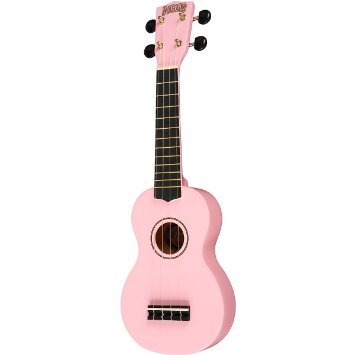
\includegraphics[width=5cm]{../img/ukulele.jpg}
\end{Slide}


% subjekt och predikat -> public static void: https://www.youtube.com/watch?v=1ZPaR_wH-R8


% \begin{Slide}{Koda i Scala}

%   {\footnotesize\it Melodi: McDonalds-låten}

% \begin{verbatim}

%           G         C             G          D
% Det finns stunder i livet som man alltid har kvar

%           G           C               D
% Det finns villkor och uttryck som man spar 

%         A           D             A           E
% Och där dörren står öppen finns gemenskap för fler 

% A      D      E       A
% Koda i Scala; det ger meeeeeeer! 
% \end{verbatim}

% \end{Slide}




\fi

%!TEX encoding = UTF-8 Unicode

%!TEX root = ../compendium1.tex

%!TEX encoding = UTF-8 Unicode
\chapter{Muntlig examen}\label{chapter:W14}



\part{Appendix}
\appendix
%!TEX encoding = UTF-8 Unicode
%!TEX root = ../compendium2.tex

\chapter{Terminalfönster}\label{appendix:terminal}

\section{Vad är ett terminalfönster?}

I ett terminalfönster kan man skriva kommandon som kör program och hanterar filer. När man programmerar använder man ofta terminalkommando för att kompilera och exekvera sina program.  
 
\subsubsection{Terminal i Linux}

    \begin{figure}[!b]
    \centering
    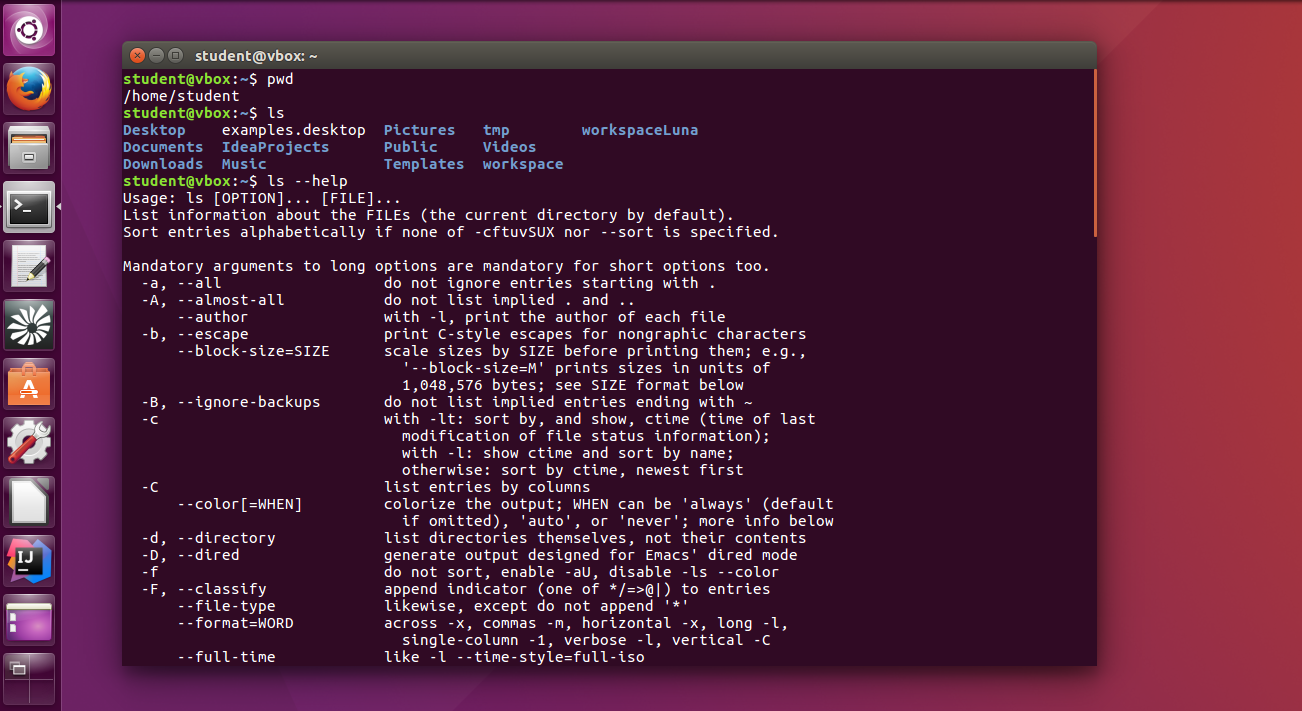
\includegraphics[width=1.0\textwidth]{../img/linux-terminal.png}
    \caption{Terminalfönster i Ubuntu öppnas med Ctrl+Alt+T.}
    \label{fig:terminal:linux}
    \end{figure}

I Ubuntu trycker du lättast \textbf{Ctrl+Alt+T} eller sök efter ''terminal'' i app-menyn.  Då öppnas ett fönster med en blinkande markör som visar att det är redo att ta emot dina textkommando. Ett exempel på kommando är \texttt{ls} som skriver ut en lista med filer i det aktuella biblioteket, så som visas i fig. \ref{fig:terminal:linux}.

Det som visas i ett terminalfönster sköts av ett \textbf{kommandoskal} \Eng{command shell}, som är redo att ta emot kommando efter en prompt som slutar med ett \texttt{\$}-tecken. När du skriver ett kommando och trycker Enter anropar kommandoskalet en kommandotolk som tolkar och utför dina kommandon. Om ett kommando inte kan tolkas, skrivs ett felmeddelande. 

Det finns många användbara kortkommando, varav de viktigaste visas i tabell \ref{fig:terminal:shortcuts}. Det är bra om du lär dig dessa kortkommandon utantill så att ditt arbete i terminalen går snabbt och smidigt.

\begin{table}[H]
\renewcommand{\arraystretch}{1.15}
\begin{tabular}{@{}r | l}
pil upp/ner & bläddra i kommandohistoriken \\
Tab & ''auto-complete'', fyll i resten baserat på vad du skrivit hittills \\
Tab Tab & två tryck på Tab listar flera alternativ, om så finnes \\
Ctrl+A & ''ahead'', flytta markören till början av raden \\
Ctrl+E & ''end'', flytta markören till slutet av raden \\
Ctrl+K & ''kill'', ta bort tecken från markören till radens slut\\
Ctrl+U & ''undo'', ta bort tecken från markören till början av raden \\
Ctrl+Y & ''yank'', sätt in det som senast togs bort\\
Ctrl+Z & ''zleep'', stoppa pågående process, skriv sedan \texttt{bg} för bakgrundskörning\\
Ctrl+L & rensa terminalfönstret\\
Ctrl+D & avsluta kommandoskalet \\
\end{tabular}
    \caption{Viktiga kortkommandon i Linux terminalfönster.}
    \label{fig:terminal:shortcuts}
\end{table}

\noindent Ctrl+C orsakar normalt ett avbrott av pågående process, men om du vill att Ctrl+C ska vara ''Copy'' som vanligt för att kopiera markerad text, kan du ställa om detta med terminalförnstrets  meny ''Edit $\rightarrow$ Keyboard Shortcuts'', eller liknande.




 
\subsubsection{PowerShell, Cmd och Linux i Microsoft Windows}
Microsoft Windows är inte Linux-baserat, men i kommandotolken \textbf{Powershell} finns alias definierade för några vanliga Linux-kommandon, inkluderat \texttt{ls}, \texttt{cd} och \texttt{pwd}. 
Du startar Powershell t.ex. genom att trycka på Windows-knappen och skriva \texttt{powershell}. 
Du kan också, medan du bläddrar bland filer, klicka på filnamnsraden överst i filbläddraren och skriva \texttt{powershell} och tryck Enter; då startas Powershell i aktuellt bibliotek. Ändra gärna typsnitt och bakgrundsfärg med hjälp av fönstrets menyer, så att det blir lättare för dig att läsa vad som skrivs.

Det finns även i Windows den ursprungliga kommandotolken \textbf{Cmd} med helt andra kommandon. Till exempel skriver man i Cmd kommandot \texttt{dir} i stället för \texttt{ls} för att lista filer. 

I Windows 10 kan du (numera, om du installerad senaste uppdateringarna av Windows) även köra Ubuntu-terminalen med hjälp av Windows Linux Subsystem (WSL). Se vidare här om hur du kan installera WSL under Windows 10: 

\url{https://ubuntu.com/wsl} 

Läs mer här: \href{https://www.omgubuntu.co.uk/2020/03/windows-10-linux-kernel-update}{www.omgubuntu.co.uk/2020/03/windows-10-linux-kernel-update}



\subsubsection{Terminal i Apple macOS/OS X}


Apple OS X och macOS är Unix-baserade operativsystem. De flesta vanliga terminalkommandon som fungerar i Linux fungerar också under Apple OS X och macOS. Du startar ett terminalfönster i Apples operativsystem genom att klicka på förstoringsglaset uppe till höger, skriva \texttt{terminal}, och trycka Enter.

\section{Vad är en path/sökväg?}\label{terminal:path}

När du skriver ett kommando i terminalen, eller kör vilket program som helst på din dator, behöver operativsystemet identifera i vilken fil programmets maskinkod ligger innan programmet kan köras. 

Lokaliseringen av filer sker med hjälp av en \textbf{sökväg} \Eng{path}, som anger en position i filsystemet. Ofta betraktas filsystemet som ett upp-och-ned-vänt träd, och kallas därför även ''filträdet''. Den ''översta'' positionen kallas ''rot'' \Eng{root} och betecknas med ett enkelt snedstreck \texttt{/}. Kataloger som ligger i kataloger utgör förgreningar i trädet. En sökväg pekar ut vägar genom trädet som behövs för att nå ''löven'', som utgörs av själva filerna.

Du kan se var ett program ligger i Linux med hjälp av kommandot \texttt{which} enligt nedan.\footnote{Skriv \texttt{ gcm ls } i Windows Powershell för motsvarighet till \texttt{ which ls } \\ Eller skriv \texttt{ New-Alias which get-command } för tillgång till kommandot \texttt{which} i Powershell. \\ \href{http://stackoverflow.com/questions/63805/equivalent-of-nix-which-command-in-powershell}{stackoverflow.com/questions/63805/equivalent-of-nix-which-command-in-powershell}} Listan med bibliotek i sökvägen avskiljs med snedstreck.
\begin{REPLnonum}
$ which java
/usr/lib/jvm/oracle_jdk8/bin/java
$ which ls
/bin/ls
\end{REPLnonum}

En sökväg kan vara \textbf{absolut} eller \textbf{relativ}. En absolut sökväg utgår från roten och visar hela vägen från rot till destination, t.ex. \texttt{/usr/bin/firefox}, medan en relativ sökväg utgår från aktuellt bibliotek (där du ''står'') och börjar \textit{inte} med ett snedstreck.

Alla operativsystem håller reda på en mängd olika sökvägar för att kunna hitta speciella filer i filträdet. Dessa sökvägar lagras i s.k. \textbf{miljövariabler} \Eng{environment variables}. Det finns en \textit{speciell} miljövariabel som heter kort och gott \textbf{PATH}, i vilken alla sökvägar till de program finns, som ska vara tillgängliga för din användaridentitet direkt för exekvering genom sina filnamn, \textit{utan} att man behöver ange absoluta sökvägar. 

Du kan i Linux se vad som ligger i din PATH med kommandot \code{ echo $PATH } medan man i Windows Powershell skriver \code{$env.Path} där det bara är första bokstaven som ska vara en versal. I Linux separeras biblioteken i sökvägen med kolon, medan Windows använder semikolon.

Ibland kan du behöva uppdatera din PATH för att program som du installerat och ska bli allmänt tillgängliga. Detta görs på lite olika sätt i olika operativsystem, för Linux se t.ex. här:
\href{http://stackoverflow.com/questions/14637979/how-to-permanently-set-path-on-linux}{stackoverflow.com/questions/14637979/how-to-permanently-set-path-on-linux}

När man anger sökvägar finns några tecken med speciell betydelse:

\begin{tabular}{r  p{0.8\textwidth}}
\code|~| & ''tilde'', din hemkatalog \\
\code|/| & ''slash'', snedstreck anger filträdets rot om det finns i början av sökvägen, men utgör biblioteksavskiljare inuti sökvägen \\
\code|.| & en punkt anger aktuellt bibliotek, där du ''står'' \\
\code|..| & två punkter anger ett steg ''upp'' i filträdet \\
\code|"| & omgärda en sökväg med citationstecken, först och sist, om den innehåller annat än engelska bokstäver, t.ex. blanktecken\\
\code|\ | & \textit{backslash+blanktecken} används för att beteckna mellanslag i sökvägar som \textit{inte} omgärdas av citationstecken\\
\end{tabular}

\section{Några viktiga terminalkommando}

I tabell \ref{fig:terminal:commands} finns en lista med några viktiga terminalkommando som är bra att lära sig utantill.

En introduktion till LTH:s datorer med exempel på hur du använder vanliga Linux-kommandon finns i denna skrift \url{http://www.ddg.lth.se/perf/unix/} som används i introduktionsveckan för nybörjare på datateknikprogrammet vid LTH.

På sajten \url{http://ss64.com/} finns en mer omfattande lista med användbara terminalkommando och tillhörande förklaringarför för Linux (Bash), Windows (Powershell, Cmd) och Apple OS X (Bash).  

\begin{table}[H]
\renewcommand{\arraystretch}{1.25}
   
\begin{tabular}{@{}r | l}
\texttt{ls} & lista filer i aktuellt bibliotek (alltså där du ''står'')\\
\texttt{ls} \textit{p}  & lista filer i biblioteket  \textit{p} \\
\texttt{ls -A} & lista alla filer i aktuellt bibliotek, även gömda \\
\texttt{man ls} & manual för kommandot \texttt{ls}; testa även \texttt{man} för andra kommandon! \\
\texttt{cd} \textit{p} & ''change directory'', ändra aktuellt bibliotek till \textit{p}\\
\texttt{pwd} & ''print working directory'', skriv ut sökväg för aktuellt bibliotek \\
\texttt{cp} \textit{p1 p2} & ''copy'', kopiera filen med path \textit{p1} till en ny fil kallad \textit{p2} \\
\texttt{mv} \textit{p1 p2} & ''move'', byt namn på filen \textit{p1} till \textit{p2}  \\
\texttt{rm} \textit{p} & ''remove'', ta bort filen \textit{p}\\
\texttt{rm -r} \textit{p} & ''remove recursive'', ta bort biblioteket \textit{p} med allt innehåll; var försiktig!\\
\texttt{mkdir} \textit{p} & ''make dir'', skapa ett nytt bibliotek \textit{p}\\
\texttt{cat} \textit{p1 p2}& ''concatenate'', skriv ut hela innehållet i en eller flera filer \textit{p1 p2 etc.}\\
\texttt{less} \textit{p}& skriv ut innehållet i filen \textit{p}, en skärm i taget\\
\texttt{wget} \textit{url}&ladda ner \textit{url}, t.ex. \texttt{ wget http://cs.lth.se/pgk/ws -o ws.zip}\\
\texttt{unzip} \textit{p}& packa upp \textit{p}, t.ex. \texttt{ unzip ws.zip}\\
\end{tabular}

    \caption{Några viktiga terminalkommando i Linux. Med \textit{p}, \textit{p1}, \textit{p2}, etc.  avses en absolut eller relativ sökväg \Eng{path}, se avsnitt \ref{terminal:path}.}
    \label{fig:terminal:commands}

\end{table}


%!TEX encoding = UTF-8 Unicode
%!TEX root = ../compendium.tex

\chapter{Editera}\label{appendix:edit}
\section{Vad är en editor?}

En editor används för att redigera programkod. Det finns många olika editorer att välja på. Erfarna utvecklare lägger ofta mycket energi på att lära sig att använda favoriteditorns kortkommandon och specialfunktioner, eftersom detta påverkar stort hur snabbt kodredigeringen kan göras. 

En bra editor har \textbf{syntaxfärgning} för språket du använder, så att olika delar av koden visas i olika färger. Då går det lättare att läsa och hitta i koden. 

I en integrerad utvecklingsmiljö (se appendix \ref{appendix:ide}) finns en inbyggd editor som, förutom syntaxfärgning, har fler avancerade funktioner. 

\section{Välj editor}

I tabell \ref{editor:popular-editors} visas en lista med några populära editorer. Det är en stor fördel om en editor finns på flera plattformar så att du har nytta av dina inövade färdigheter när du behöver växla mellan olika operativsystem. 

Om du inte vet vilken du ska välja, börja med \textit{gedit}, som inte är så avancerad, men därför lätt att kommna igång med. När du sedan är redo att investera din lärtid i en mer avancerad editor rekommenderas \textit{Atom}, eftersom den är öppen, gratis och finns för Linux, Windows och macOS. 

Det är är också bra att lära sig åtminståne de mest basala kommandona i editorn \textit{vim} eftersom denna  editor kan köras direkt i terminalen, även vid fjärrinloggning, och finns förinstallerad i de flesta Linux-system.
%!TEX encoding = UTF-8 Unicode
%!TEX root = ../compendium.tex

\chapter{Kompilera och exekvera}\label{appendix:compile}

\section{Vad är en kompilator?}

En \textbf{kompilator} \Eng{compiler} är ett program som läser programtext och översätter den till exekverbar maskinkod, så som visas i figur \ref{fig:appendix:compiler}. Programtexten som kompileras kallas källkod och utgörs av text som följer reglerna för ett programmeringsspråk, till exempel Scala eller Java. 

\begin{figure}[H]
\centering
\begin{tikzpicture}[node distance=1.8cm, scale=1.5]
\node (input) [startstop] {\bf\sffamily Källkod};
\node(inptext) [right of=input, text width=2cm, xshift=1.5cm]{För\\människor};
\node (compile) [process, below of=input] {\bf\sffamily Kompilator};
%\node(explain) [right of=compile, text width=5cm, xshift=3.0cm]{Översätter från källkod till maskinkod};
\node (output) [startstop, below of=compile] {\bf\sffamily Maskinkod};
\node(outtext) [right of=output, text width=2cm, xshift=1.5cm]{För\\maskiner};
\draw [arrow] (input) -- (compile);
\draw [arrow] (compile) -- (output);
\end{tikzpicture}
    \caption{En kompilator översätter från källkod till maskinkod.}
    \label{fig:appendix:compiler}
\end{figure}




Vissa kompilatorer genererar kod som kan köras av en processor direkt, medan andra kompilatorer genererar ett mellanformat som tolkas under exekveringen. Det senare är fallet med Java och Scala, vilket möjliggör att programmet kan kompileras en gång för alla plattformar och sedan kan programmet köras på all de processorer till vilka en s.k. virtuell maskin för Java finns \Eng{Java Virtual Machine, JVM}. Den kod som genereras av en kompilator som kodgenererar för JVM kallas \textbf{bytekod}.

Om kompileringen inte lyckas skriver kompilatorn ut ett felmeddelande och ingen maskinkod genereras. Det är inte lätt att bygga en kompilator som ger bra felmeddelanden i alla lägen, men felmeddelandet ger oftast goda ledtrådar till felorsaken efter att man lärt sig tolka det programmeringsspråksspecifika vokabulär som kompilatorn använder.

Även om programmet kompilerar utan felmeddelande och genererar exekverbar maskinkod, är det vanligt att programmet ändå inte fungerar som det är tänkt. Ibland är det mucket svårt att lista ut vad problemet beror på och man kan behöver göra omfattande undersökningar av vad som händer under körningen, genom att t.ex. skriva ut olika variablers värden eller på annat sätt ändra koden och se vad som händer. Denna process kallas felsökning eller avlusning \Eng{debugging}, och är en väsentlig del av all systemutveckling. 

En uttömmande testning av ett större program, som kör programmets \textit{alla} möjliga exekveringsvägar, är i praktiken omöjlig att genomföra inom rimlig tid, då antalet kombinationsmöjligheter växer mycket snabbt med storleken på programmet. 
Därför är kompilatorn ett mycket viktigt hjälpmedel. Med hjälp av den analys och de kontroller som görs av kompilatorn kan många buggar, som annars vore mycket svåra att hitta, undvikas och åtgärdas i kompileringsfasen, redan \textit{innan} man exekverar programmet. 


\section{Java JDK}

Scala, Java och flera andra språk använder Java-plattformen som exekveringsmiljö. Om man inte bara vill köra program som andra har utvecklat, utan även utveckla egna program som fungerar i denna miljö, behöver man installera Java Develpment Kit (JDK). Detta utvecklingspaket innehåller flera delar, bland annat:

\begin{itemize}

\item Kompilatorn \texttt{javac} kompilerar Java-program till bytekod som lagras i klassfiler med filnamnsändelsen \texttt{.class}.

\item Exekveringsmiljön Java Runtime Enviroment (JRE) med kommandot \texttt{java} som drar igång den virtuella javamaskinen (Java Virtual Machine) som kan ladda och exekvera bytekod lagrade i klassfiler.

\item Programmet \texttt{jar} som packar ihop många sammanhörande klassfiler till en enda jar-fil som lätt kan distribueras via nätet och sedan köras med \texttt{java}-kommandot på alla maskiner med JRE. 

\item Programmet \texttt{javap} som läser klassfiler och skriver ut vad de innehåller i ett format som kan läsas av människor (ett sådant program kallas disassembler).

\item I JDK ingår också en mycket stor mängd färdiga programbibliotek med stöd för nätverkskommunikation, filhantering, grafik, kryptering och en massa annat som behövs när man bygger moderna system. 

\end{itemize}  

\noindent Du kan läsa mer om Java och dess historik här: \\
\href{https://en.wikipedia.org/wiki/Java_(programming_language)}{https://en.wikipedia.org/wiki/Java\_(programming\_language)}

\subsection{Kontrollera om du har JDK installerat}\label{appendix:compile:check-jdk}

Öppna ett terminalfönster (se appendix \ref{appendix:terminal}) och skriv (observera det avslutande c:et i \texttt{javac}):
\begin{REPLnonum}
javac -version
\end{REPLnonum}
Då ska ungefär följande skrivas ut (där siffran 101 kan vara något annat):
\begin{REPLnonum}
javac 1.8.0_101
\end{REPLnonum}
Om utskriften säger att javac saknas, installera JDK8 enl. nedan.

Du kanske redan har enbart Java Runtime Environment (JRE) installerad, men inte JDK. Då saknar du javakompilatorn javac m.m. och behöver installera JDK, se nedan. Du kan kolla om du har JRE genom att skriva \texttt{java -version} (alltså utan c efter java). Eller så har du redan JDK installerad men inte rätt bibliotek i din PATH; se vidare nedan ang. uppdatering av PATH.



\subsection{Installera JDK}\label{appendix:compile:install-jdk}

Det finns flera JDK-distributioner att välja mellan, varav Oracle JDK och Azul Zulu OpenJDK är två exempel. Oracle JDK har störst spridning och är förinstallerad på LTH:s datorer. För att installera JDK på din egen dator behöver du gå igen flera steg, som behöver anpassas efter det operativsystem du kör, enligt nedan. 
På kurshemsidan under ''Verktyg'' finns kompletterande instruktioner:  \url{http://cs.lth.se/pgk/verktyg} 


Din användaridentitet behöver ha administratörsrättigheter för att du ska kunna genomföra installationen.



\subsubsection{Linux} 
För Ubuntu: läs först noga igenom och följ sedan dessa instruktioner till punkt och pricka: \\ \href{http://www.webupd8.org/2012/09/install-oracle-java-8-in-ubuntu-via-ppa.html}{www.webupd8.org/2012/09/install-oracle-java-8-in-ubuntu-via-ppa.html}

För andra Linux-distributioner, kör detta i terminalen (funkar även i Ubuntu men du får med detta kommando inte Oracles aningen snabbare JVM): \\ \texttt{sudo apt-get install openjdk-8-jdk}

\subsubsection{Windows/macOS}

\begin{enumerate}
\item Installera senaste JDK från Oracle. Om du inte har installerat JDK förr på din dator så be gärna någon kurskamrat med erfarenhet av detta att assistera dig medan du följer stegen nedan. 

\begin{enumerate}
\item Surfa till Oracles hemsida för Java SE här: \\ \url{http://www.oracle.com/technetwork/java/javase/downloads/}

\item Klicka på rubriken ''Java SE 8u101 / 8u102'' och på nästa sida klicka på knappen ''Accept License Agreement'' i listan under rubriken ''Java SE Development Kit 8u101''. (Siffrorna 101 eller 102 kan vara annorlunda om senare versioner tillkommit.)

\item Välj rätt version av operativsystem (Windows x64 eller Mac OS X). Det är viktigt att du väljer x64, d.v.s 64-bitarsvarianten som gäller för alla moderna datorer.

\item Klicka på länken och en stor fil kommer laddas ner till din dator.

\item Installera när filen laddats färdigt. 

\end{enumerate}

\item Uppdatera PATH, så att du får tillgång till alla kommando i terminalen:
\begin{itemize}
\item För Windows görs detta enklast genom att ladda ner och sedan köra denna fil genom att dubbelklicka på den: \\ \url{https://github.com/lunduniversity/introprog/raw/master/tools/windows-jdk-set-path.bat}
\item För macOS, läs här: \\ \href{https://docs.oracle.com/javase/8/docs/technotes/guides/install/mac_jdk.html}{docs.oracle.com/javase/8/docs/technotes/guides/install/mac\_jdk.html}

\item Om något krånglar, be om hjälp. Om du vill veta mer om PATH-uppdatering för java, läs här:\\ \url{https://java.com/sv/download/help/path.xml} \\
Om du kör engelska menyer byt \texttt{sv} mot \texttt{en} i adressen ovan.  Du kan ta reda på vilken katalog som ska läggas in sist i din PATH efter ett semikolon genom att bläddra bland dina systemfiler och undersöka var JDK har installerats; i Windows antagligen något liknande detta (kolla exakt vilket versionsnummer du har): \code|C:\Program Files\Java\jdk1.8.0_101\bin|
\end{itemize}

\item Starta om datorn. Det är först efter att en ny användarinloggning initierats, som PATH-tilldelningen får effekt.

\item Kontrollera att \texttt{javac} fungerar enligt avsnitt \ref{appendix:compile:check-jdk}.
\end{enumerate}


\section{Scala}

Scala använder JDK som exekveringsmiljö, men erbjuder ytterligare verktyg specifika för Scala. I utvecklingspaketet för Scala ingår bl.a. kompilatorn \texttt{scalac} och även ett interaktivt kommandoskal kallat Scala REPL där du kan testa din Scala-kod rad för rad och se vad som händer direkt. 

De flesta av kursens övningar görs i Scala REPL, medan laborationerna kräver kompilering av lite större program.

Du hittar mer om Scalas historik och annan bakgrundsinformation här: \mbox{%
 \href{https://en.wikipedia.org/wiki/Scala_(programming_language)}{en.wikipedia.org/wiki/Scala\_(programming\_language)}
}

\subsection{Installera Scala}

Scala finns förinstallerat på LTH:s datorer. Du installerar Scala-kompilatorn och den interaktiva kodexperimentmiljön Scala REPL på din egen dator enligt nedan. 

\begin{enumerate}
\item Kontrollera att du har JDK installerad enligt avsnitt \ref{appendix:compile:check-jdk} och installera vid behov enligt avsnitt \ref{appendix:compile:install-jdk}.
\item Surfa till denna hemsida för nedladdning av Scala 2.11.8: \\ \url{http://scala-lang.org/download/2.11.8.html}
\item Klicka på ''Download'' av den variant som är relevant för ditt operativsystem och spara filen:

\begin{enumerate}
\item \textbf{Linux Ubuntu}: Filen heter \texttt{scala-2.11.8.deb} och installeras genom att dubbelklicka på filen eller via terminalkommandot:\\ \code{sudo apt install ~/Downloads/scala-2.11.8.deb} \\ anpassa sökvägen ovan efter var du sparade filen 
\item \textbf{Windows}: Filen heter \texttt{scala-2.11.8.msi} och installationen startas med ett dubbelklick. Följ instruktionerna. Installationsprogrammet uppdaterar även din PATH åt dig och allt bör fungera efter omstart.
\item \textbf{macOS}: Filen heter \texttt{scala-2.11.8.tgz} och kan packas upp på lämpligt ställe med terminalkommandot \texttt{tar -xvzf scala-2.11.8.tgz} och sedan är det underkatalogen \texttt{bin} som ska inkluderas i din PATH. \TODO klura ut säkraste rådet för path-uppdatering på mac.
\end{enumerate}
Kontrollera att terminalkommandot \texttt{scala} fungerar för att starta Scala REPL:
\end{enumerate}
\begin{REPLnonum}
$ scala
Welcome to Scala 2.11.8 (Java HotSpot(TM) 64-Bit Server VM, Java 1.8.0_101).
Type in expressions for evaluation. Or try :help.

scala> println("hej")
hej

scala>
\end{REPLnonum}
 

\subsection{Scala Read-Evaluate-Print-Loop (REPL)}\label{appendix:compile:REPL}

För många språk, t.ex. Scala och Python, finns det en interaktiv tolk som gör det möjligt att exekvera enstaka programrader och direkt se effekten. En sådan tolk kallas Read-Evaluate-Print-Loop eftersom den läser en rad i taget och översätter till maskinkod som körs direkt.    

\TODO Kortkommandon: Ctrl+K etc.

\TODO :paste








%!TEX encoding = UTF-8 Unicode
%!TEX root = ../compendium.tex

\chapter{Integrerad utvecklingsmiljö}\label{appendix:ide}

\section{Vad är en integrerad utvecklingsmiljö?}

En integrerad utvecklingsmiljö \Eng{integrated development environment, IDE} samlar ett flertal verktyg, inklusive en avancerad \textbf{editor} (se appendix \ref{appendix:edit}), för att skapa, köra och testa program. Det finns flera utvecklingsmiljöer att välja mellan, som kan användas för både Scala och Java.

En IDE ger stöd för \textbf{kodkomplettering} \Eng{code completion} där tillgängliga metoder visas i en lista och resten av ett namn kan fyllas efter att du skrivit de första bokstäverna i namnet. En IDE kan hjälpa dig med formattering och även skapa skelettkod utifrån \textbf{kodmallar} \Eng{code templates}. Med \textbf{felindikering} \Eng{error highlighting} får du understrykning av vissa fel direkt i koden och ibland kan du även få hjälp med förslag på åtgärder för att rätta till enkla fel. Funktioner för \textbf{avlusning} \Eng{debugging} hjälper dig att felsöka medan du kör din kod. Med funktioner för \textbf{omstrukturering} \Eng{refactoring} av kod får du hjälp av editorn i samarbete med kompilatorn att göra omfattande strukturförändringar i många kodfiler samtidigt, t.ex. namnbyten med hänsyn taget till språkets synlighetsregler.  

Alla dessa avancerade funktioner kan öka produktiviteten avsevärt, men samtidigt tar de tid att lära sig och en IDE kan kräva mycket datorkraft och viss väntetid jämfört med en vanlig, fristående editor. I början kan all funktionalitet upplevas som överväldigande och det kan vara svårt att hitta i alla menyer och inställningar. Ska man bara skriva ett litet, enkelt program, eller göra några mindre ändringar, är det många som föredrar en fristående, snabbstartad kodeditor före en fullfjädrad, tungrodd IDE. Å andra sidan kan en IDE med kodkomplettering vara till stor hjälp när man ska lära sig ett nytt api och experimentera med en okänd kodmassa.

I kursen använder vi flera utvecklingsmiljöer. På första labben använder vi Kojo (avsnitt \ref{appendix:ide:kojo}) som är en IDE speciellt anpassad på nybörjare. I laborationerna senare i kursen kan du välja att använda någon av de professionella utvecklingsmiljöerna Eclipse (avsnitt \ref{appendix:ide:eclipse}) eller IntelliJ (avsnitt \ref{appendix:ide:intellij}). Om du inte vet vilken du ska välja, börja med att prova Eclipse.


\newpage

\section{Kojo}\label{appendix:ide:kojo}

Kojo%
\footnote{\href{https://en.wikipedia.org/wiki/Kojo_(programming_language)}{en.wikipedia.org/wiki/Kojo\_(programming\_language)}}
 är en integrerad utvecklingsmiljö för Scala som är speciellt anpassad för nybörjare i programmering. Kojo används i LTH:s Science Center Vattenhallen för utbildning av grundskolelärare i programmering och vid skolbesök och annan besöksverksamhet, i vilken lärare och studenter vid LTH arbetar som handledare. Kojo är fri öppenkällkod och utvecklingen leds av Lalit Pant.

Kursens första laboration genomförs med hjälp av Kojo, men Kojo kan med fördel användas som komplement till Scala REPL och annan IDE under hela kursens gång. Medan Scala REPL lämpar sig för korta kodsnuttar, och en fullfjädrad, professionell IDE har funktioner för att hantera riktigt stora programmeringsprojekt, passar Kojo bra för mellanstora program. I Kojo finns även lätttillgängliga bibliotek som gör tröskeln lägre att programmera rörlig grafik och enkla spel.   


\begin{figure}[H]
\centering
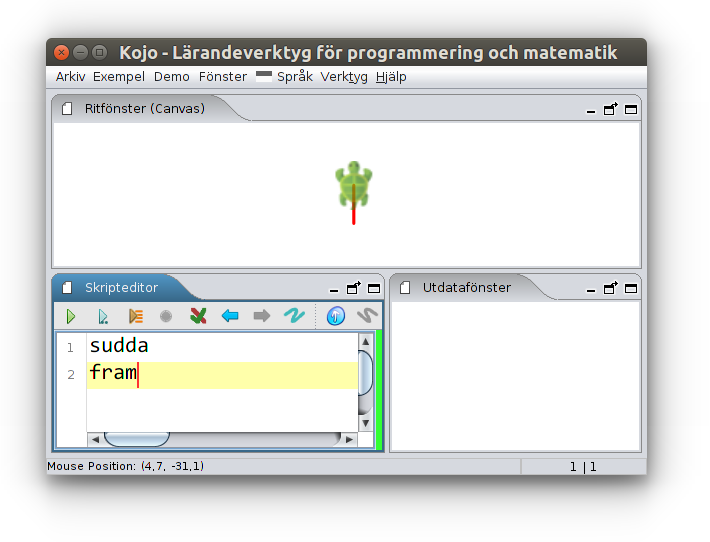
\includegraphics[width=0.8\textwidth]{../img/kojo/kojo.png}
\caption{Den nybörjarvänliga utvecklingsmiljön Kojo för Scala på svenska.}
\label{fig:appendix:ide:kojo}
\end{figure} 

\subsection{Installera Kojo}

Kojo är förinstallerat på LTH:s datorer och körs igång med kommandot \texttt{kojo}. För instruktioner om hur du installerar Kojo på din egen dator se här:\\
\href{http://www.lth.se/programmera/installera/}{lth.se/programmera/installera}

Kojo kräver att \texttt{java} finns på din dator. Eftersom du behöver tillgång till JDK i kursen, är det lika bra att installera hela JDK direkt (och inte bara JRE, så som beskrivs å länken ovan); se vidare hur du gör detta i avsnitt \ref{appendix:compile:install-jdk}. 
%\href{http://www.kogics.net/kojo-download}{www.kogics.net/kojo-download}


\subsection{Använda Kojo}

När du startar Kojo första gången, välj ''Svenska'' i språkmenyn och starta om Kojo. Därefter fungerar grafikfunktionerna på svenska enligt tabell \ref{table:kojo:functions}. När du startat om Kojo inställt på Svenska ser programmet ut ungeför som i figur \ref{fig:appendix:ide:kojo} på sidan \pageref{fig:appendix:ide:kojo}.


Det finns ett antal användbara kortkommando som du hittar i menyerna i Kojo. Undersök speciellt Ctrl+Alt+Mellanslag som ger autokomplettering baserat på det du börjat skriva.


{\small\renewcommand{\arraystretch}{1.45}
\begin{longtable}{@{}p{0.42\textwidth} p{0.55\textwidth}}

\caption{Några av sköldpaddans funktioner. Se även \href{http://lth.se/programmera}{lth.se/programmera}}\label{table:kojo:functions}\\

\emph{Svenska/Engelska} & \emph{Vad händer?}  \\ \hline
%!TEX encoding = UTF-8 Unicode
%!TEX root = ../compendium2.tex

\chapter{Kojo}\label{appendix:kojo}

\section{Vad är Kojo?}

Kojo%
\footnote{\href{https://en.wikipedia.org/wiki/Kojo_(programming_language)}{en.wikipedia.org/wiki/Kojo\_(programming\_language)}}
 är en integrerad utvecklingsmiljö för Scala som är speciellt anpassad för programmeringsundervisning i grundskolan. Kojo används i LTH:s Science Center Vattenhallen för utbildning av grundskolelärare i programmering och vid skolbesök och annan besöksverksamhet, i vilken lärare och studenter vid LTH arbetar som handledare. 
 
 Kojo är öppen källkod och utvecklingsgemenskapen leds av Lalit Pant från Indien. I Kojo finns även lättillgängliga bibliotek som gör tröskeln lägre att programmera rörlig grafik och enkla spel.

Under kursens första laboration använder vi grafikbiblioteket i Kojo för att illustrera grundläggande begrepp, så som sekvens, alternativ, repetition och abstraktion.  


\begin{figure}[H]
\centering
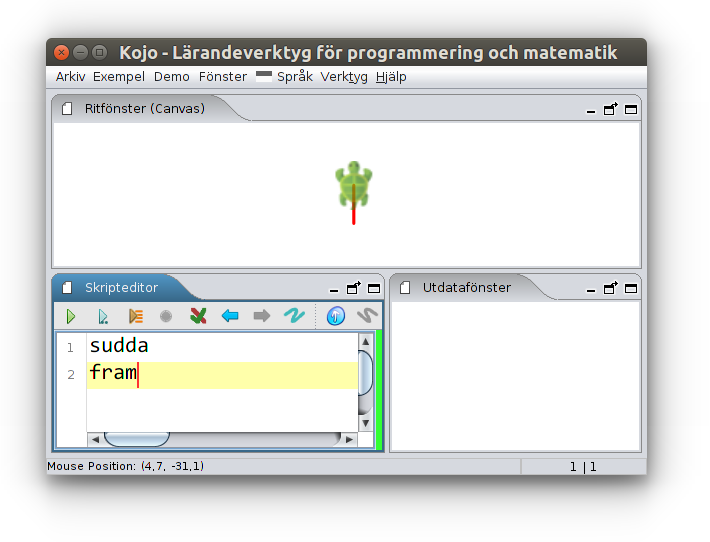
\includegraphics[width=0.8\textwidth]{../img/kojo/kojo.png}
\caption{Den nybörjarvänliga utvecklingsmiljön Kojo för Scala på svenska.}
\label{fig:appendix:ide:kojo}
\end{figure}

\section{Använda grafikbiblioteket i Kojo}\label{appendix:ide:kojo:install}

Kojo bygger på den beprövade pedagogiska idén med sköldpaddsgrafik \Eng{turtle graphics}\footnote{\url{https://en.wikipedia.org/wiki/Turtle_graphics}}, där du skriver program som styr en sköldpadda med en penna under magen. När sköldpaddan rör sig bildas ett streck av valfri färg på skärmen. Beroende på hur du bestämmer att sköldpaddan ska röra sig och vilken färg du bestämmer att pennan ska ha, kan du skapa olika intressanta bilder och samtidigt lära dig om programmeringens grunder.

Under kursens första laboration ska du använda grafikbiblioteket i Kojo tillsammans med editorn VS \code{code} och \code{scala-cli} i terminalen (se appendix \ref{appendix:terminal} och \ref{appendix:compile}). Ladda ner filen \texttt{kojo.scala} från \url{https://cs.lth.se/pgk/kojolib} och spara i en ny katalog med hjälp av din webbläsare, eller via dessa kommandon:

\begin{REPLnonum}
> mkdir w01-kojo
> cd w01-kojo
> curl -o kojolib.scala -sL https://cs.lth.se/pgk/kojolib
\end{REPLnonum}

Nu kan du starta Scala REPL och rita med Kojo så här:

\begin{REPLnonum}
> scala-cli repl .
Welcome to Scala 3.1.2 (17.0.2, Java OpenJDK 64-Bit Server VM).
Type in expressions for evaluation. Or try :help.
                                                                                                                               
scala> fram; höger; fram; vänster

\end{REPLnonum}

Du kan starta VS \code{code} i aktuellt bibliotek så här:
\begin{REPLnonum}
> code .
\end{REPLnonum}

Skriv nedan progam i VS \code{code} och spara det i samma katalog som den tidigare nedladdade filen, under ett nytt valfritt filnamn, t.ex. \code{rita.scala}:

\begin{Code}
@main def rita =
  fram; höger
  fram; vänster
\end{Code}

Kör ditt fristående program med:
\begin{REPLnonum}
> scala-cli run .
\end{REPLnonum}

Du ska nu få upp ett fönster som heter Kojo Canvas med en sköldpadda som ritat två streck. När du stänger fönstret så avslutas programmet. Prova fler sköldpaddsfunktioner enligt tabell \ref{table:kojo:functions}.

I stället för att ladda ned filen \code{kojolib.scala} så kan du placera dess innehåll på lämpligt ställe i ditt program enligt nedan. Observera att raden som börjar med \code{//> using lib} ska vara en enda lång rad utan radbrytningar. Raden med \code{export} gör Kojos kommandon tillgängliga utan prefix:
\begin{CodeSmall}[breaklines=true]
//> using scala "3"
//> using lib "net.kogics:kojo-lib:0.1.1,url=https://github.com/lunduniversity/introprog/releases/download/kojo-lib-0.1.1/kojo-lib-0.1.1.jar"

export net.kogics.kojo.Swedish.*, padda.*, CanvasAPI.*, TurtleAPI.*
\end{CodeSmall}


\noindent Scala-koden för den svenska paddans api finns här: \\
%\href{https://github.com/litan/kojo/blob/master/src/main/scala/net/kogics/kojo/lite/i18n/svInit.scala}{github.com/litan/kojo/blob/master/src/main/scala/net/kogics/kojo/lite/i18n/svInit.scala} \\
\href{https://github.com/litan/kojo-lib/blob/main/src/main/scala/net/kogics/kojo/i18n/Swedish.scala}{github.com/litan/kojo-lib/blob/main/src/main/scala/net/kogics/kojo/i18n/Swedish.scala}


%Kojo kräver (numera) \emph{inte} att \texttt{java} finns på din dator utan kommer med en egen JVM. 
%Eftersom du behöver tillgång till JDK i kursen, är det lika bra att installera hela JDK direkt (och inte bara JRE, så som beskrivs å länken ovan); se vidare hur du gör detta i avsnitt \ref{appendix:compile:install-jdk}.
%\href{http://www.kogics.net/kojo-download}{www.kogics.net/kojo-download}


{\small\renewcommand{\arraystretch}{1.4}
\begin{longtable}{@{}p{0.42\textwidth} p{0.55\textwidth}}

\caption{Ett urval av funktioner i Kojo. Se även \href{http://lth.se/programmera}{lth.se/programmera}}\label{table:kojo:functions}\\

\emph{Svenska/Engelska} & \emph{Vad händer?}  \\ \hline
\code|sudda| \newline \code|clear| & Ritfönstret suddas \\
\code|fram| \newline \code|forward()| & Paddan går framåt 25 steg. \\
\code|fram(100)| \newline \code|forward(100)| & Paddan går framåt 100 steg. \\
\code|höger| \newline \code|right(90)| & Paddan vrider sig 90 grader åt höger. \\
\code|höger(45)| \newline \code|right(45)| & Paddan vrider sig 45 grader åt höger. \\
\code|vänster| \newline \code|left(90)| & Paddan vrider sig 90 grader åt vänster. \\
\code|vänster(45)| \newline \code|left(45)| & Paddan vrider sig 45 grader åt vänster. \\
\code|hoppa| \newline \code|hop| & Paddan hoppar 25 steg utan att rita. \\
\code|hoppa(100)| \newline \code|hop(100)| & Paddan hoppar 100 steg utan att rita. \\
\code|hoppaTill(100, 200)| \newline \code|jumpTo(100, 200)| & Paddan hoppar till läget (100, 200) utan att rita. \\
\code|gåTill(100, 200)| \newline \code|moveTo(100, 200)| & Paddan vrider sig och går till läget (100, 200). \\
\code|hem| \newline \code|home| & Paddan går tillbaka till utgångsläget (0, 0). \\
\code|öster| \newline \code|setHeading(0)| & Paddan vrider sig så att nosen pekar åt höger. \\
\code|väster| \newline \code|setHeading(180)| & Paddan vrider sig så att nosen pekar åt vänster. \\
\code|norr| \newline \code|setHeading(90)| & Paddan vrider sig så att nosen pekar uppåt. \\
\code|söder| \newline \code|setHeading(-90)  | & Paddan vrider sig så att nosen pekar neråt. \\
\code|mot(100,200)| \newline \code|towards(100, 200)| & Paddan vrider sig så att nosen pekar mot läget (100, 200) \\
\code|sättVinkel(90)| \newline \code|setHeading(90)| & Paddan vrider nosen till vinkeln 90 grader. \\
\code|vinkel| \newline \code|heading| & Ger vinkelvärdet dit paddans nos pekar. \\
\code|sakta(5000)| \newline \code|setAnimationDelay(5000) | & Gör så att paddan ritar jättesakta. \\
\code|suddaUtdata| \newline \code|clearOutput| & Utdatafönstret suddas. \\
\code|utdata("hej")| \newline \code|println("hej")| & Skriver texten \texttt{hej} i utdatafönstret. \\
\code|val t = indata("Skriv")| \newline \code|val t = readln("Skriv:")| & Väntar på inmatning efter ledtexten \texttt{Skriv} och sparar den inmatade texten i t.  \\
\code|textstorlek(100)| \newline \code|setPenFontSize(100)| & Paddan skriver med jättestor text nästa gång du gör skriv. \\
\code|båge(100, 90)| \newline \code|arc(100, 90)| & Paddan ritar en båge med radie 100 och vinkel 90. \\
\code|cirkel(100)| \newline \code|circle(radie)| & Paddan ritar en cirkel med radie 100. \\
\code|synlig| \newline \code|visible| & Paddan blir synlig. \\
\code|osynlig| \newline \code|invisible| & Paddan blir osynlig. \\
\code|läge.x| \newline \code|position.x| & Ger paddans x-läge \\
\code|läge.y| \newline \code|position.y| & Ger paddans y-läge \\
\code|pennaNer| \newline \code|penDown| & Sätter ner paddans penna så att den ritar när den går. \\
\code|pennaUpp| \newline \code|penUp| & Lyfter upp paddans penna så att den INTE ritar när den går. \\
\code|pennanÄrNere| \newline \code|penIsDown| & Kollar om pennan är nere eller inte. \\
\code|färg(rosa)| \newline \code|setPenColor(pink)| & Sätter pennans färg till rosa. \\
\code|fyll(lila)| \newline \code|setFillColor(purple)| & Sätter ifyllnadsfärgen till lila. \\
\code|fyll(genomskinlig)| \newline \code|setFillColor(noColor)| & Gör så att paddan inte fyller i något när den ritar. \\
\code|bredd(20)| \newline \code|setPenThickness(20)| & Gör så att pennan får bredden 20. \\
\code|sparaStil| \newline \code|saveStyle| & Sparar pennans färg, bredd och fyllfärg. \\
\code|laddaStil| \newline \code|restoreStyle| & Laddar tidigare sparad färg, bredd och fyllfärg. \\
\code|sparaLägeRiktning| \newline \code|savePosHe| & Sparar pennans läge och riktning \\
\code|laddaLägeRiktning| \newline \code|restorePosHe| & Laddar tidigare sparad riktning och läge \\
\code|siktePå| \newline \code|beamsOn| & Sätter på siktet. \\
\code|sikteAv| \newline \code|beamsOff| & Stänger av siktet. \\
\code|bakgrund(svart)| \newline \code|setBackground(black)| & Bakgrundsfärgen blir svart. \\
\code|bakgrund2(grön,gul)| \newline \code|setBackgroundV(green, yellow)| & Bakgrund med övergång från grönt till gult. \\
\code|upprepa(4){fram; höger}| \newline \code|repeat(4){forward; right}| & Paddan går fram och svänger höger 4 gånger. \\
\code|avrunda(3.99)| & Avrundar 3.99 till 4.0 \\
\code|slumptal(100)| & Ger ett slumptal mellan 0 och 99. \\
\code|slumptalMedDecimaler(100)| & Ger ett slumptal mellan 0 och 99.99999999 \\
\code|systemtid| & Ger nuvarande systemklocka i sekunder. \\
\code|räknaTill(5000)| & Kollar hur lång tid det tar för din dator att räkna till 5000. \\


\end{longtable}
}%end small


\section{Kojo Desktop}

Kojo finns som fristående skrivbordsapplikation, kallad Kojo Desktop. Kojo Desktop innehåller en egen editor med syntaxfärgning för Scala, men fungerar ännu så länge bara för Scala 2. En av de synligaste skillnaderna mellan Scala 2 och Scala 3 är att klammerparenteser vid flerradiga funktioner är nödvändiga i Scala 2, medan Scala 3 har valfria klammerparenteser. Så om du använder Kojo Desktop behöver du komma ihåg att omgärda sekvenser av rader som hör ihop med \code|{| och \code|}|. 

Kojo Desktop är förinstallerat på LTH:s datorer och körs igång med terminalkommandot \texttt{kojo} eller via applikationsmenyn.  För instruktioner om hur du installerar Kojo Desktop på din egen dator se här: \href{http://www.lth.se/programmera/installera/}{lth.se/programmera/installera}

När du startar Kojo första gången, välj ''Svenska'' i språkmenyn och starta om Kojo. Därefter fungerar grafikfunktionerna på svenska enligt tabell \ref{table:kojo:functions}. När du startat om Kojo inställt på svenska ser programmet ut ungefär som i figur \ref{fig:appendix:ide:kojo} på sidan \pageref{fig:appendix:ide:kojo}.

Det finns ett antal användbara kortkommando som du hittar i menyerna i Kojo Desktop. Undersök speciellt Ctrl+Alt+Mellanslag som ger autokomplettering baserat på det du börjat skriva.

\section{Kojo i Webbläsaren}

En begränsad variant av Kojo finns tillgänglig för programmering direkt i din webbläsare här: \url{http://kojo.lu.se/}

När du trycker på play-knappen så kompileras din kod på en server till Javascript via ScalaJS och därefter körs Javascript-koden i din webbläsare. 
Kojo på webben är också ännu så länge begränsad till Scala 2 och kräver att du omgärdar sekvenser av rader som hör ihop med \code|{| och \code|}|.


\section{Mer om Kojo}

I detta dokument finns en enkel introduktion till Kojo: \\ ''Introduction to Kojo'' \url{http://www.kogics.net/kojo-ebooks#intro}


\hline
\end{longtable}
}%end small

\noindent Scala-koden för den svenska paddans api finns här: \\
\href{https://bitbucket.org/lalit_pant/kojo/src/tip/src/main/scala/net/kogics/kojo/lite/i18n/svInit.scala}{bitbucket.org/lalit\_pant/kojo/src/tip/src/main/scala/net/kogics/\\kojo/lite/i18n/svInit.scala}




\newpage

\section{Eclipse och ScalaIDE}\label{appendix:ide:eclipse}

Eclipse%
\footnote{\href{https://en.wikipedia.org/wiki/Eclipse_(software)}{en.wikipedia.org/wiki/Eclipse\_(software)}}
är en professionell IDE som stödjer många olika programmeringsspråk. Eclipse är skriven i Java och bygger vidare på ett utvecklingsprojekt som initierades av IBM. Eclipse är ett fritt och öppet projekt som numera kontrolleras av en oberoende stiftelse.

Till Eclipse finns en insticksmodul \Eng{plug-in} som kallas ScalaIDE och erbjuder stöd för Scala med tillhörande standardbibliotek.

Eclipse är en omfattande och avancerad programmeringsmiljö med många funktioner och inställningar. Det finns även en omfattande uppsättning insticksmoduler och tilläggsprogram som underlättar utveckling av t.ex. webbprogram, databaser och mycket annat. 

I detta avsnitt ges länkar till installation samt tips om hur du kommer igång med att använda Eclipse och ScalaIDE. Det går ganska snabbt att lära sig grunderna, men det kräven en viss ansträngning att lära sig de mer avancerade funktionerna. Det finns omfattande resurser på nätet som hjälper dig vidare. 


\subsection{Installera Eclipse Mars och ScalaIDE}\label{appendix:ide:eclipse:install}

Eclipse med ScalaIDE är förinstallerat på LTH:s datorer och startas med kommandot \texttt{scalaide} i ett terminalfönster.

ScalaIDE fungerar med Eclipse-versionerna \textit{Luna} och \textit{Mars} (men i skrivande stund fungerar ScalaIDE ännu \textit{inte} med den allra senaste versionen kallad \textit{Neon}). 

För att installera ScalaIDE på din egen dator, följ nedan instruktioner: 

\begin{enumerate}
\item Kontrollera enligt avsnitt \ref{appendix:compile:check-jdk} att du har \texttt{java} installerat och installera vid behov JDK enligt avsnitt \ref{appendix:compile:install-jdk}.

\item Installera Eclipse version \textbf{Mars}, varianten för \textbf{Java Developers} som återfinns på denna sida: \\ \url{https://www.eclipse.org/downloads/packages/release/Mars/2} \\ som är den \textit{andra} varianten i listan (alltså inte Java EE). Följ dessa steg:
\begin{enumerate}
\item Klicka på den \textbf{64-bit}-variant som passar ditt operativsystem.
\item Filen som laddas ner heter något som liknar (beroende på OS): \\ \texttt{eclipse-java-mars-2-win32-x86\_64.zip} 
\\ Det kan ta lång tid att ladda ner filen som är på ca 170MB. Om du klickar på \textit{''select a mirror''} kan du välja en svensk sajt för att ladda ner snabbare. 

\item Dubbelklicka på filen för att packa upp den, vilket kan ta många minuter. Du får, när upppackningen är klar, ett bibliotek med en fungerande Eclipse-installation som du kan placera var du vill. Kör du Windows, lägg den förslagsvis här:\\ 
\code|C:\eclipse\eclipse-java-mars-2-win32-x86_64|

\item för Ubuntu Linux finns kompletterande installationsanvisningar här, som ger dig en ikon i app-menyn m.m.: 
\\ \url{http://askubuntu.com/questions/26632/how-to-install-eclipse}
\end{enumerate}

\item Installera Scala IDE inifrån%
\footnote{Det finns på ScalaIDE-hemsidan möjlighet att ladda ner en Eclipse-variant med färdiginstallerad ScalaIDE-plugin, men då får du i skrivande stund den gamla versionen Eclipse \textit{Luna}, varför du rekommenderas att, enligt instruktionerna här, själv installera ScalaIDE inifrån Eclipse \textit{Mars}, som är den senaste Eclipse-versionen för vilken ScalaIDE fungerar.}
 Eclipse enligt nedan steg:
\begin{enumerate}
\item Starta Eclipse, t.ex. genom att köra igång den exekverbara filen som ligger i underbiblioteket \texttt{eclipse}, i Windows heter den \texttt{eclipse.exe} medan den exekverbara filen i Linux heter \texttt{eclipse} utan filändelse.

\item Välj i frågerutan som dyker upp, någon plats för \textit{workspace} (kvittar vilken just nu, kan ändras senare).

\item Klicka på menyn \textit{Help} $\rightarrow$ \textit{Install new software}.

\item Klicka på \textit{Add}-knappen till höger och skriv: \\ \textit{''ScalaIDE for Scala 2.11''} i \textit{Name}-fältet och ange denna adress i \textit{Location}-fältet: \\
  {\small\mbox{\url{http://download.scala-ide.org/sdk/lithium/e44/scala211/stable/site}}} \\
  och klicka \textit{OK}.
  
\item Du får nu upp en lista med alternativ. Kryssa för alternativet
\\ {\frame{\checkmark}}~~\textit{Scala IDE for Eclipse} \\ och klicka \textit{Next} och sedan \textit{Next} igen och acceptera licensvillkoren och klicka \textit{Finish}.

\item Låt installationen ta sin tid och starta sedan om Eclipse när installationen är färdig. 

\item När Eclipse är igång igen visas en dialog som föreslår att du ska köra \textit{Setup Diagnostics}. Gör detta och välj \textit{Use recommended default settings}. Ändra även i filen \textbf{eclipse.ini} för höja den övre minnesgränsen. Det gör du genom att ändra på den rad i filen som börjar med \texttt{-Xmx}. Hur mycket du ska tillåta som max beror på hur mycket minne du har, men ge minst 1 gigabyte för smidig körning, genom att skriva så här på relevant rad i filen \textbf{eclipse.ini}: \\
\texttt{-Xmx1G } \\


\item Kompletterande information finns här, inklusive en video som visar installationsproceduren och hur man kommer igång med ett ''hello world''-program: \\ \url{http://scala-ide.org/download/current.html}


\end{enumerate}


\end{enumerate}

\noindent I nästa avsnitt beskrivs några rekommenderade anpassningar som du kan göra bland de omfattande inställningsmöjligheterna för Eclipse.

\newpage

\subsection{Anpassa Eclipse och ScalaIDE}\label{subsection:appendix:ide:eclipse:tweaks}

\newcommand\Menu[1]{\textit{#1}}
\newcommand\MenuArrow[1]{\Menu{#1}~$\rightarrow$~}
\newcommand\FramedCheckmark[1]{~\frame{\checkmark}~~\textbf{#1}}
\newcommand\FramedUnchecked[1]{$\Box$~\textbf{#1}}
\newcommand\Button[1]{\fbox{\textbf{#1}}}
\newcommand\EclipsePrefs{\MenuArrow{Window}\MenuArrow{Preferences}}
\newcommand\EclipsePrefsGeneral{\EclipsePrefs\MenuArrow{General}}


Förutom maxminneshöjningen i filen \texttt{eclipse.ini}, som finns i installationskatalogen för Eclipse, till minst \texttt{-Xmx1G } (se föregående avsnitt), är det bra att göra några ytterligare anpassningar av Eclipse och ScalaIDE för att få en snabbare och smidigare utvecklingsmiljö. Du hittar inställningarna i menyn \EclipsePrefs ... uppe till höger i Eclipse-fönstret.



\begin{enumerate}
\item \EclipsePrefsGeneral 
\\ Markera \FramedCheckmark{Show Heap Status} så får du se minnesanvändningen i en liten ruta i nederdelen av fönstret, vilket hjälper dig att upptäcka om minnesbegränsningen i filen \texttt{eclipse.ini} är en flaskhals vid stora projekt och många öppna fönster. Klicka sedan \Button{Apply} längst ner.

\item \label{item:scala-perspective} \EclipsePrefsGeneral\MenuArrow{Editors}\MenuArrow{Perspective}  
\\ Markera \textit{Scala} i listan med perspektiv och klicka på knappen 
 \\ \Button{Make default} till höger och sedan på knappen \Button{Apply} längst ner.

\item \EclipsePrefsGeneral\MenuArrow{Editors}\MenuArrow{TextEditors}
\\ Markera \FramedCheckmark{Insert spaces for tabs} så att du slipper specialtecken som kan tolkas olika av olika editorer. Klicka sedan \Button{Apply} längst ner.

\item \EclipsePrefsGeneral\MenuArrow{Editors}\MenuArrow{TextEditors}
\\ \MenuArrow{Spelling} Avmarkera \FramedUnchecked{Enable spell checking} för att slippa att svenska namn och svenska kommentarer markeras som felstavade. Om du senare jobbar med ett projekt helt på engelska, kan du med fördel markera denna kryssruta igen. Klicka sedan \Button{Apply} längst ner.

\item \EclipsePrefsGeneral\MenuArrow{Editors}\MenuArrow{Webbrowser}
\\ Markera \FramedCheckmark{Use external web browser} för att köra din vanliga webbläsare när du klickar på länkar. Klicka sedan \Button{Apply} längst ner.
  
\item  \EclipsePrefs\MenuArrow{Scala}\MenuArrow{Compile}
\\ I fliken \textbf{Standard} markera dessa kryssrutor för att få extra varningar: \\
\begin{tabular}{l @{}l @{}l}
\textit{deprecation} & \FramedCheckmark{} & varnar vid användning av föråldrad kod som snart utgår \\
\textit{feature}     & \FramedCheckmark{} & påminner om import vid användning av avancerad kod  \\
\textit{unchecked}   & \FramedCheckmark{} & ger tips vid speciella problem med generiska typer \\
\end{tabular}\\
och klicka sedan på knappen \Button{Apply} längst ner.

\item \EclipsePrefs\MenuArrow{Java}\MenuArrow{Compiler}\MenuArrow{Errors/Warnings}
\\ Veckla ut listan \textbf{Potential programming problems} och sätt \textbf{Resource leak} till alternativet \textbf{Ignore}, så slipper du varningar vid användning \jcode{Scanner} i Java. Klicka sedan \Button{Apply} längst ner.

\end{enumerate}

\noindent Ovan anpassningar är rekommenderade men inte nödvändiga och du kan gärna välja att göra andra anpassningar som passar just dig. Skriv då gärna ner vilken inställning du ändrat, så att du hittar tillbaka om du ångrar dig. 

Du hittar tips om fler inställningar för att anpassa ScalaIDE här: \\
\url{http://scala-ide.org/docs/current-user-doc/advancedsetup}



\subsection{Använda Eclipse och ScalaIDE}\label{appendix:ide:eclipse:use}

Ett grundläggande koncept i Eclipse är \textbf{workspace}. Ett workspace utgör ett arbetsområde kopplat till en katalog i ditt filsystem där du kan arbeta med ett eller flera \textbf{projekt}. Ett projekt innehåller i sin tur dina källkodsfiler och klassfiler etc. i en specifik katalogstruktur som Eclipse skapar när du editerar, kompilerar och kör dina projekt. 

\subsubsection{Starta och välja workspace}\label{subsubsection:start:eclipse}

När du startar Eclipse måste du välja vilket workspace du vill använda innan du kommer vidare. När du kör igång Eclipse första gången, klicka OK enligt det förslag som ges. Du kan senare växla workspace genom menyn \MenuArrow{File}\Menu{Switch Workspace}. Om katalogen du anger inte redan finns, kommer den att skapas och initieras med de filer Eclipse behöver.

I figur \ref{fig:appendix:eclipse:welcome} visas välkomstfliken i Eclipse med sina länkar till funktionsöversikt och olika handledningar. Stäng välkomstfliken genom att klicka på flikens kryss eller på ikonen \textit{Workbench}. Då kommer du vidare till den normala arbetsytan i Eclipse. Du kan få tillbaka välkomstfliken igen via menyn \MenuArrow{Help}\Menu{Welcome}. 

\begin{figure}[H]
\centering
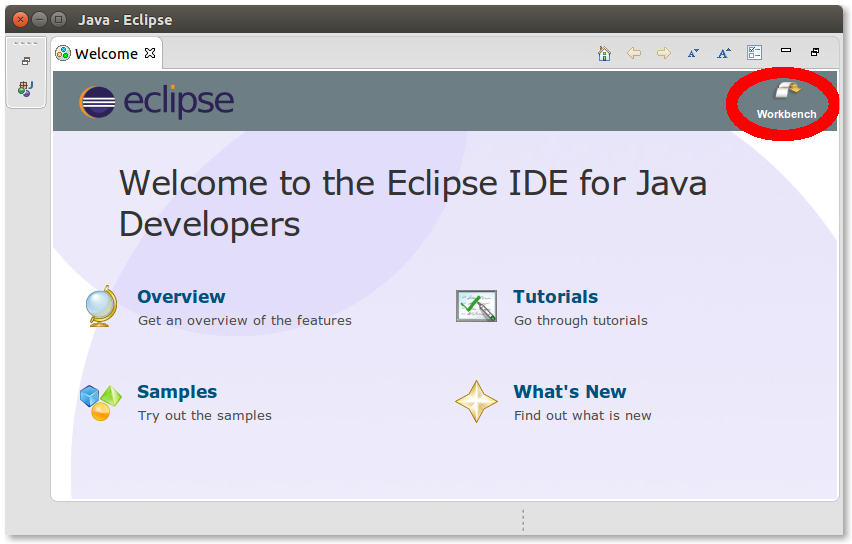
\includegraphics[width=1.0\textwidth]{../img/eclipse/eclipse-welcome.png}
\caption{Välkomstfliken för Eclipse, som nås via menyn \MenuArrow{Help}\Menu{Welcome}. Gå vidare genom att klicka på \textit{Workbench}.}
\label{fig:appendix:eclipse:welcome}
\end{figure}

\subsubsection{Välja perspektiv och visa olika vyer}

Eclipse-fönstret kan innehålla många underfönster i olika flikar, så kallade \textbf{views} eller vyer, som kan arrangeras på olika vis efter hur du vill ha dem. Vilka vyer som syns och hur de placeras beror på vilket s.k. \textbf{perspective} som är aktivt.  Figur \ref{fig:appendix:eclipse:open-perspective} visar arbetsytan med olika vyer i Java-perspektivet. 

Du kan byta till Scala-perspektivet genom att trycka på 
\includegraphics[scale=0.75]{../img/eclipse/eclipse-perspective-button.png} eller genom menyn \MenuArrow{Window}\MenuArrow{Perspective}\MenuArrow{Open Perspective}\MenuArrow{Other...}\Menu{Scala}.
Du kan anpassa inställningarna så att Scala blir \textit{default perspective}, se steg \ref{item:scala-perspective} i avsnitt \ref{subsection:appendix:ide:eclipse:tweaks} på sidan \pageref{subsection:appendix:ide:eclipse:tweaks}.

Stäng vyerna \textit{Task List} och \textit{Outline} om du vill ha mer plats till de övriga vyerna för paketnavigering, editering och utdata. Du kan öppna stängda vyer igen genom menyn \MenuArrow{Window}\Menu{Show View}. 

\begin{figure}
\centering
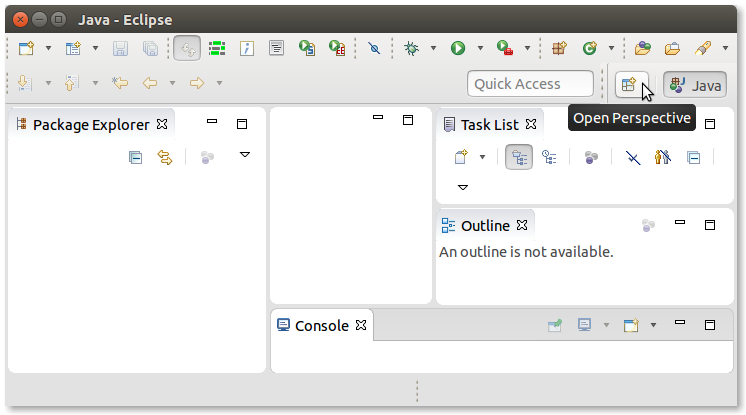
\includegraphics[width=1.0\textwidth]{../img/eclipse/eclipse-open-perspective.png}
\caption{Arbetsytan i Eclipse. Du kan växla mellan Scala- och Java-perspektivet genom att klicka på perspektivvalsknappen.}
\label{fig:appendix:eclipse:open-perspective}
\end{figure}

\subsubsection{Hello World}\label{subsubsection:eclipse:hello-world}

Efter att du öppnat Eclipse med ScalaIDE i ett tomt workspace och valt Scala-perspektivet enligt föregående avsnitt, kan du skapa ditt första projekt med ett \textit{''Hello World''}-program enligt stegen nedan.

\begin{enumerate}
\item Högerklicka i \Menu{Package Explorer} och välj \MenuArrow{New}\Menu{Scala Project}, varefter en dialogruta visas. 

\item Fyll i namnet \texttt{hello} i fältet \Menu{Project Name} och klicka \Button{Finish}.

\item Högerklicka igen i \Menu{Package Explorer} och välj \MenuArrow{New}\Menu{Scala Object}, varefter en ny dialogruta visas. 

\item Fyll i namnet \texttt{hi} i fältet \Menu{Project Name} och klicka \Button{Finish}.

\item Du får nu i editorvyn ett kodskellet med \code{object hi}.

\item Börja skriv \code{main} som visas i figur \ref{fig:appendix:eclipse:complete-main} och tryck Ctrl+Mellanslag för att aktivera kodkomplettering \Eng{code completion}. Då får du upp en lista med alternativ. Välj det översta alternativet \texttt{main} varefter ett kodskellet med en main-metod klistras in automatiskt i din kod.

\begin{figure}
\centering
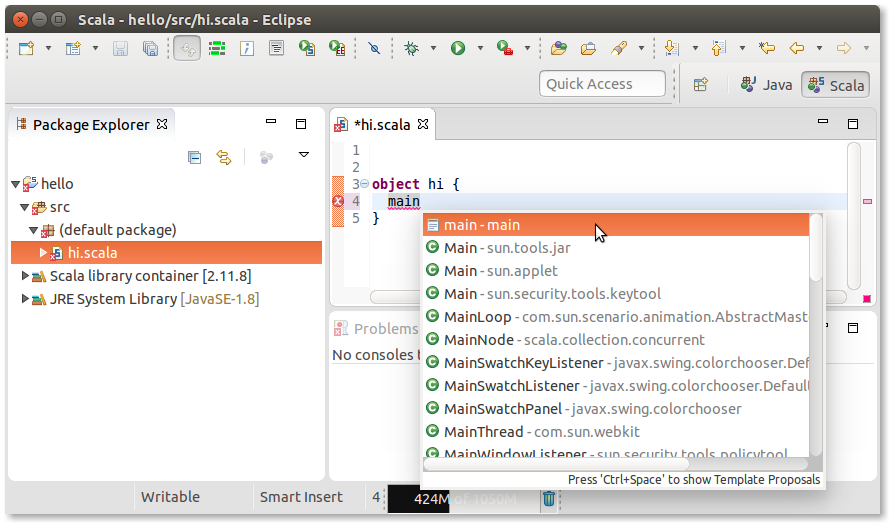
\includegraphics[width=1.0\textwidth]{../img/eclipse/eclipse-complete-main.png}
\caption{Aktivera kodkomplettering med Ctrl+Mellanslag efter ordet \code{main}.}
\label{fig:appendix:eclipse:complete-main}
\end{figure}

\item Fyll i lämplig utskriftstext i ett \code{println}-anrop så att din \code{main}-metod blir så som visas i editorfliken i figur \ref{fig:appendix:eclipse:hello-world}.

\begin{figure}[H]
\centering
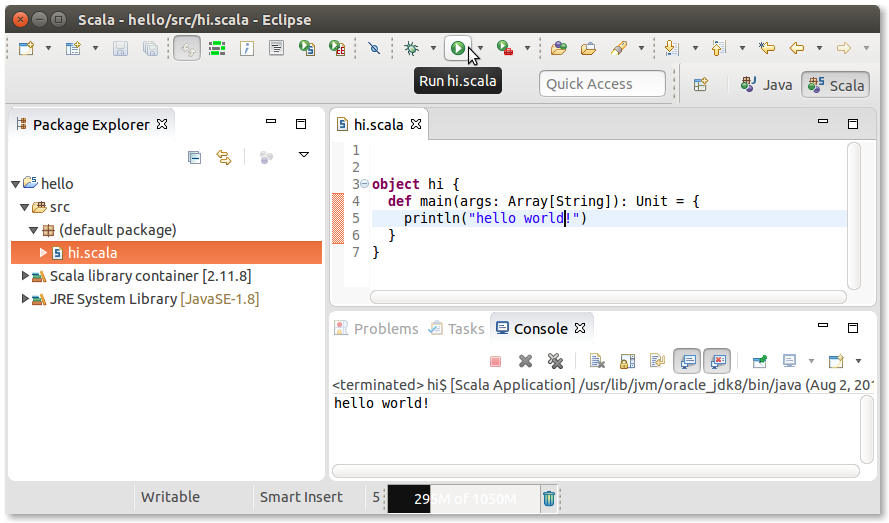
\includegraphics[width=1.0\textwidth]{../img/eclipse/eclipse-hello-world.png}
\caption{Skriv klart \code{main}-metoden och kör ditt program med play-knappen.}
\label{fig:appendix:eclipse:hello-world}
\end{figure}

\item Kör ditt program genom att trycka på den gröna play-knappen, som muspekaren i figur \ref{fig:appendix:eclipse:hello-world} pekar på. Du kan också trycka F11 för att köra igång din app, efter att du vid första körningen i dialogen \textit{Select Preferred Launcher} markerat  \FramedCheckmark{Use configuration specific settings} och valt alternativet \textit{Scala Application (new debugger) Launcher}. 

\end{enumerate}




\subsubsection{Ladda ner kursens workspace och importera projekt till labbarna}

Det finns en zip-fil med ett workspace med projekt för flera av kursens laborationer som du kan ladda ner och importera i Eclipse. Följ stegen nedan.

\begin{enumerate}
\item Ladda ner kursens workspace här: \url{http://cs.lth.se/pgk/ws}

\item Packa upp filen på lämpligt ställe.

\item Starta Eclipse med ScalaIDE-plugin (se startinstruktioner på sidan \pageref{subsubsection:start:eclipse}). 

\item Växla workspace till biblioteket du nyss packade upp, ungefär som i figur \ref{fig:eclipse:ide:open} och klicka \Button{OK}.
\begin{figure}[H]
\centering
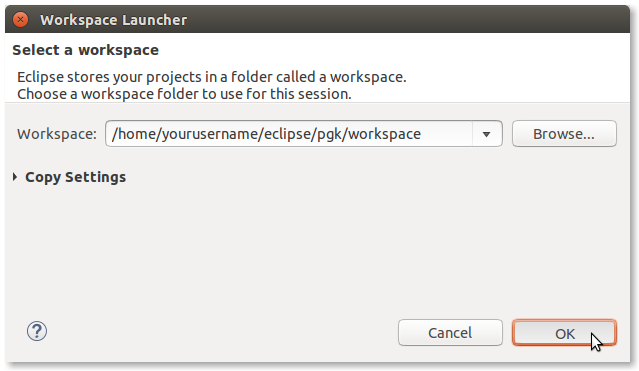
\includegraphics[width=1.0\textwidth]{../img/eclipse/eclipse-select-workspace.png}
\caption {Öppna kursens workspace genom att bläddra till biblioteket där du packade upp filen som du laddat ned från: \url{http://cs.lth.se/pgk/ws} }
\label{fig:eclipse:ide:open}
\end{figure}

\item Stäng välkomstfliken för att komma vidare till workbench (se figur \ref{fig:appendix:eclipse:welcome} på sidan \pageref{fig:appendix:eclipse:welcome}). Det ser då ut ungefär som i figur~\ref{fig:appendix:eclipse:open-perspective} på sidan \pageref{fig:appendix:eclipse:open-perspective}. Det syns ännu inget i \textit{Package Explorer} då vi ännu inte importerat något projekt. 

\item Innan du går vidare, säkerställ att du har Scala-perspektivet aktiverast. Du kan växla till Scala-perspektivet genom att trycka på 
\includegraphics[scale=0.75]{../img/eclipse/eclipse-perspective-button.png} eller genom menyn \MenuArrow{Window}\MenuArrow{Perspective}\MenuArrow{Open Perspective}\MenuArrow{Other...}\Menu{Scala}.
Du kan anpassa inställningarna så att Scala blir \textit{default perspective}, se steg \ref{item:scala-perspective} i avsnitt \ref{subsection:appendix:ide:eclipse:tweaks} på sidan \pageref{subsection:appendix:ide:eclipse:tweaks}.


\item Högerklicka i \textit{Package Explorer} och välj \Menu{Import...}, se Fig.~\ref{fig:eclipse:import}, eller välj menyn \MenuArrow{File}\Menu{Import...}. 

\begin{figure}[H]
\centering
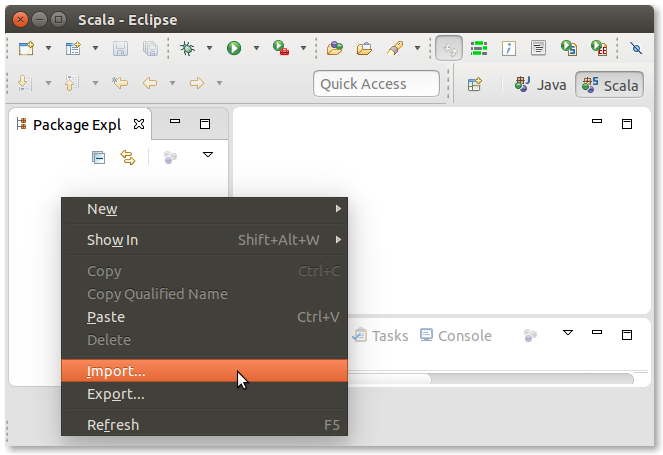
\includegraphics[width=1.0\textwidth]{../img/eclipse/eclipse-import.png} 

\caption {Välj \Menu{Import}-menyn för att importera existerande projekt.}
\label{fig:eclipse:import}
\end{figure}

\item Nu öppnas \Menu{Import}-dialogen som visas i figur \ref{fig:eclipse:import-existing}. Öppna mappen \Menu{General}, markera \textbf{Existing Projects into Workspace} och klicka \Button{Next}.



\begin{figure}[H]
\centering
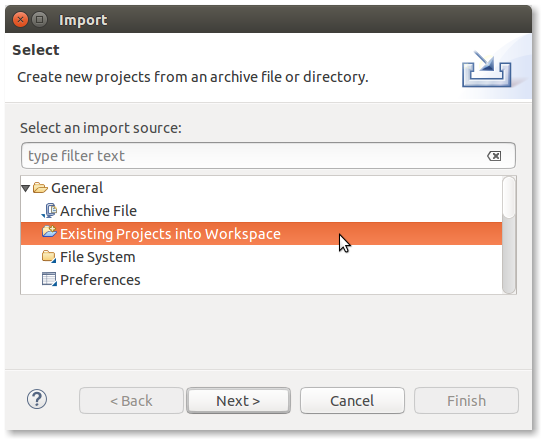
\includegraphics[width=0.75\textwidth]{../img/eclipse/eclipse-import-existing.png} 

\caption {Välj att importera existerande projekt under \Menu{General}.}
\label{fig:eclipse:import-existing}
\end{figure}


\begin{figure}[H]
\centering
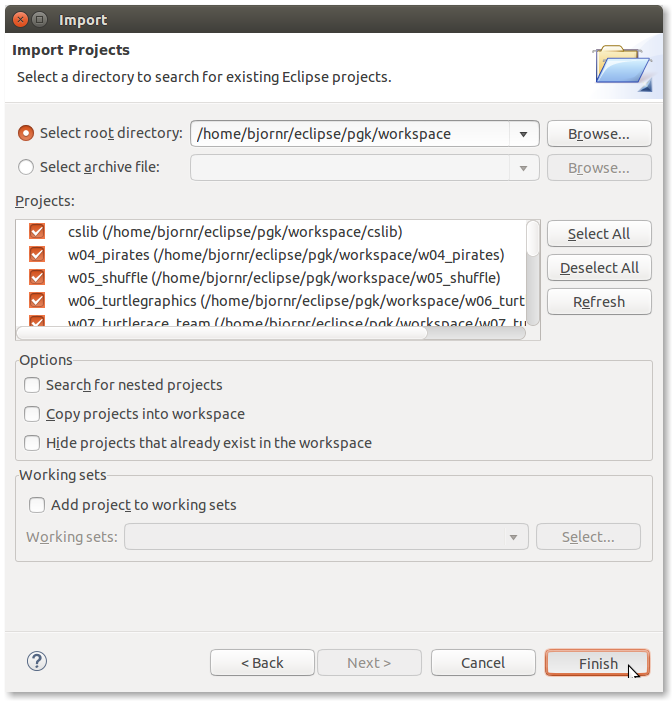
\includegraphics[width=1.0\textwidth]{../img/eclipse/eclipse-import-projects.png} 

\caption {Välj \FramedCheckmark{Select Root Directory} och klicka \Button{Browse}.}
\label{fig:eclipse:import-projects}
\end{figure}


\item Nu kommer ytterligare ett dialogfönster som visas i figure \ref{fig:eclipse:import-projects}. Med \FramedCheckmark{Select Root Directory} markerad kan du klicka \Button{Browse} för att ange workspace-mappen i ännu en dialog där du bara ska trycka \Button{Ok} utan att välja underbibliotek till workspace. När det är klart ska det se ut som i figur \ref{fig:eclipse:import-projects} där alla Eclipse-projekt \FramedCheckmark{cslib}, \FramedCheckmark{w04\_pirates}, etc. är markerade. Klicka sedan \Button{Finish}.

\item Följ ''Hello World''-instruktionerna på sidan \pageref{subsubsection:eclipse:hello-world} och skapa programmet som visas i figure \ref{fig:eclipse:pirates-hi}, genom att veckla ut projektet \textbf{w04\_pirates}, markera och högerklicka på paketet \textbf{priates}, och välja \MenuArrow{New}\Menu{Scala Object}.

\begin{figure}[H]
\centering
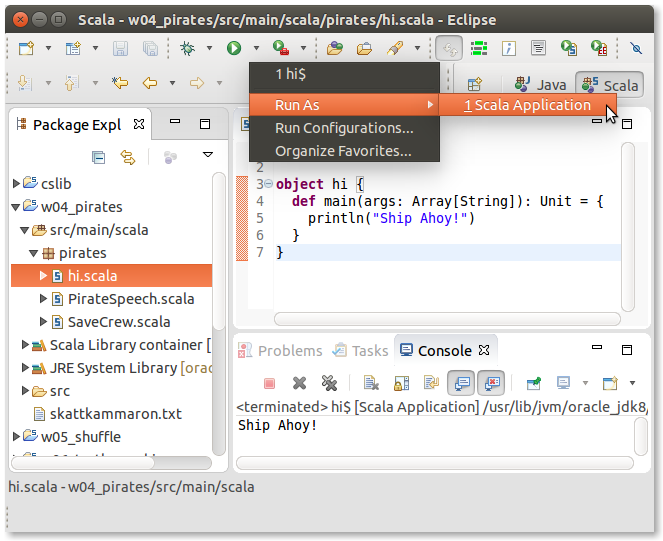
\includegraphics[width=1.0\textwidth]{../img/eclipse/eclipse-pirates-hi.png} 

\caption {Skapa ett \MenuArrow{New}\Menu{Scala Object} med kod enligt bilden.}
\label{fig:eclipse:pirates-hi}
\end{figure}


\end{enumerate}



\newpage

\section{IntelliJ IDEA}\label{appendix:ide:intellij}

IntelliJ IDEA%
\footnote{\href{https://en.wikipedia.org/wiki/IntelliJ_IDEA}{en.wikipedia.org/wiki/IntelliJ\_IDEA}}
 är en professionell IDE som stödjer många olika programmeringsspråk. IntelliJ är skriven i Java och utvecklas av det tjeckiska företaget JetBrains. 

IntelliJ IDEA finns i två varianter: en gratis gemenskapsvariant med öppenkällkodslicens \Eng{Community edition}, samt en betalvariant med stängd källkod och support-tjänster.


Till IntelliJ IDEA finns en insticksmodul \Eng{plug-in} som erbjuder stöd för Scala med tillhörande standardbibliotek..

IntelliJ IDEA är en omfattande och avancerad programmeringsmiljö med många funktioner och inställningar. Det finns även en omfattande uppsättning insticksmoduler och tilläggsprogram som underlättar utveckling av t.ex. webbprogram, databaser och mycket annat. 

I detta avsnitt ges länkar till installation samt tips om hur du kommer igång med att använda IntelliJ IDEA med Scala. Det går ganska snabbt att lära sig grunderna, men det kräven en viss ansträngning att lära sig de mer avancerade funktionerna. Det finns omfattande resurser på nätet som hjälper dig vidare. 

Google tillkännagav 2013 att företaget övergår från Eclipse till IntelliJ som den officiellt understödda utvecklingsmiljön för Android och 2014 lanserades utvecklingsmiljön AndroidStudio%
\footnote {\href{https://en.wikipedia.org/wiki/Android_Studio}{en.wikipedia.org/wiki/Android\_Studio}}
 som bygger vidare på IntelliJ. 

\subsection{Installera IntelliJ med Scala}\label{appendix:ide:intellij:install}

IntelliJ med Scala-plug-in är förinstallerat på LTH:s datorer och startas med kommandot \texttt{intellij} i ett terminalfönster.

\TODO Beskriv hur man installerar IntelliJ med Scala

\subsection{Använda IntelliJ}\label{appendix:ide:intellij:use}

\TODO 

%!TEX encoding = UTF-8 Unicode
%!TEX root = ../compendium1.tex

\chapter{Fixa buggar}\label{appendix:debug}

\begin{figure}[H]
\centering\includegraphics[width=0.85\textwidth]{../img/bug}

\caption{Den första dokumenterade buggen hittades 9 september 1947 i en Mark II Aiken Relay Calculator av Grace Hopper.\protect\footnotemark}

\end{figure}\footnotetext{\href{https://commons.wikimedia.org/w/index.php?curid=165211}{commons.wikimedia.org/w/index.php?curid=165211} Courtesy of the Naval Surface Warfare Center, Dahlgren, VA., 1988. - U.S. Naval Historical Center Online Library Photograph NH 96566-KN, Public Domain.   }


\section{Vad är en bugg?}

En bugg, även kallad lus \Eng{bug}, är en felaktighet som kan göra så att ett program inte beter sig som det är tänkt, och kan innebära oönskad utdata, att programmet kraschar, eller till och med ond bråd död.\footnote{\href{https://www.theguardian.com/technology/2016/jul/01/tesla-driver-killed-autopilot-self-driving-car-harry-potter}{www.theguardian.com/technology/2016/jul/01/tesla-driver-killed-autopilot-self-driving-car-harry-potter}}

Ursprunget till ordets användning i programmeringssammanhang är något oklar, men kan härledas till engelskans \emph{bug} som betyder insekt eller småkryp. 
Man brukar berätta att vid en felsökning av ett program som körde i en tidig dator byggd med  elektromekaniska reläer, uppdagades en död nattfjäril ihjälklämd mellan drivankaret och spolen i ett relä, som orsakade att programmet inte kunde exekveras korrekt. 



\subsection{Olika sorters fel}

När man ska lära sig mer om fel i programvarubaserade system, och hur de kan åtgärdas, är det viktigt att noga skilja på \textbf{misstag} \Eng{mistake}, \textbf{felorsak} \Eng{fault} och \textbf{felyttring} \Eng{failure}. 
Med ''misstag'' menar vi här ett fel som begås av människor (utvecklare, systemadministratörer, operatörer, användare, etc.) medan de skapar och använder ett programvarusystem. 

Det kan bli fel i olika delar av processen: 
\begin{itemize}
\item \textbf{Kravfel} uppstår medan man tänker ut vad systemet ska göra och då misstar sig angående  användarnas behov och önskemål.
\item \textbf{Designfel} uppkommer när man utformar systemets struktur på ett dåligt sätt.
\item \textbf{Implementeringsfel} begås när man programmerar och skriver felaktiga kodrader. 
\item \textbf{Testfel} förekommer vid provkörning av systemet då testkoden är felaktig och därför ger falskt alarm om ''fel'', trots att beteendet egentligen är korrekt.  
\item \textbf{Operatörsfel} sker när systemet lämnas över till de, som ska installera och köra systemet i skarp produktion, och där systemdriften \Eng{operations, ''ops''} sköts på ett sätt som får problematiska konsekvenser.
\item \textbf{Användarfel} händer då användarna ger felaktig indata, eventuellt i strid med riktlinjerna för hur systemet ska användas, som systemet inte klarar att hantera korrekt, varpå mer eller mindre allvarliga felbeteenden hos systemet följer.
\end{itemize} 
I olika delar av utvecklingsprocessen kan alltså misstag begås som, antingen omedelbart, eller någon gång i framtiden, kan orsaka fel. Men det är inte säkert att ett fel någonsin kommer att märkas. Kanske kommer de felaktiga kodraderna, som \emph{skulle} kunna orsaka ett fel, aldrig att exekveras. Eller så kommer ingen användare att någonsin vilja använda systemet så som stipuleras av (onödiga) krav. Det är alltså först när fel \emph{yttrar} sig vid exekvering som misstag märks.

Fel kan också kategoriseras utifrån \emph{hur} de upptäcks i utvecklingsprocessen. Man brukar skilja på fel upptäckta vid granskning, kompileringsfel och exekveringsfel, som diskuteras nedan:
\begin{itemize}
\item Fel upptäckta vid \textbf{granskning}. Ett effektivt sätt att upptäcka fel är att människor noga läser igenom sin egen, och andras kod och försöker leta efter möjliga problem och brister. Man blir ofta ''hemmablind'' när det gäller ens egen kod. Därför kan någon annans, oberoende granskning med ''nya, friska'' ögon vara mycket fruktbar.  I samband med kodgranskning kan man med fördel försöka bedöma  huruvida koden är lätt att läsa, lätt att ändra i eller om koden har andra viktiga kvaliteter som har betydelse för den framtida utvecklingen av koden. Ofta hittar man vid granskning även enkla programmeringsmisstag, så som felaktiga villkor och loop-räknare som inte räknas upp på rätt sätt etc.
  
\item \textbf{Kompileringsfel} uppkommer under kompilering och upptäcks tack vare kontroller som sker av  kompilatorn. 

Vid kompileringsfel får man också ofta av kompilatorn reda på \emph{var} i koden det är fel och \emph{varför} det är fel, så att sökandet efter felorsaken och åtgärdandet av misstaget underlättas. Men ibland är felmeddelandet från kompilatorn missvisande och pekar på helt fel ställe i koden, så det gäller att inte alltid lita blint på det kompilatorn skriver. Dessutom är felmeddelanden från kompilatorn ofta uttryckta i termer av språkets syntaktiska och semantiska regler och det tar tid att lära sig tolka kompilatorers felmeddelanden. Att skapa kompilatorer som ger bra felmeddelande är ett svårt problem som studeras inom den datavetenskapliga disciplinen \textit{kompilatorteknik}, vilken du kan lära mer om i kurser på avancerad nivå.

Olika programmeringsspråk erbjuder olika stora möjligheter att göra kontroller vid kompileringstid. En kompilator för ett språk med ett avancerat typsystem, som till exempel Scala, ger förhållandevis stora möjligheter att identifiera fel redan under kompileringen, medan man med ett språk med ett svagare typsystem, till exempel Javascript, får förlita sig på prestandahämmande kontroller som kompilatorn genererar i maskinkoden eller som du själv väljer att lägga in i källkoden för säkerhets skull. 
  
\item \textbf{Exekveringsfel}, även kallat körtidsfel \Eng{runtime error}, sker medan programmet körs. Det kan krävas viss, specifik indata under specifika exekveringsomständigheter (en viss processor, en viss minnesstorlek, en viss nätverkskapacitet etc.) för att ett exekveringsfel ska yttra sig. När ett exekveringsfel väl yttrar sig, kan olika saker hända:

\begin{itemize}

\item \textbf{Exekveringen ger oönskat resultat.} Det är inte säkert att ett exekveringsfel avbryter exekveringen; det är vanligt att felet ''bara'' resulterar i inkorrekt utdata eller på annat sätt ger dålig kvalitet. För att upptäcka detta innan systemet sätts i drift, är det allmän praxis att man skriver noga uttänkta \textbf{testfall} och analyserar \textbf{testresultat} från exekveringen av  testfallen i detalj genom att undersöka utdata i jämförelse med önskat resultat eller med vad som anses vara en tillräckligt hög kvalitetsnivå.

\item \textbf{Exekveringen hänger sig} \Eng{hang}. Ibland yttrar sig fel genom att inget alls ser ut att hända under exekveringen, vilket kan beror på t.ex.:  
\begin{itemize}[nolistsep]
\item en \textbf{oändlig loop}, som aldrig blir färdig, 
\item att det går \textbf{väldigt långsamt} eftersom bearbetningen av indata tar orimligt lång tid,
\item att programmet \textbf{väntar på indata} som aldrig kommer,
\item att olika jämlöpande delar av programmet väntar på varandra så att ett \textbf{dödläge} \Eng{deadlock} uppstår. 
\end{itemize}

När exekveringen hänger sig och man inte orkar vänta längre på att något ska hända, är det bara att brutalt avbryta exekveringen genom något lämpligt kommando som erbjuds i din körmiljö.\footnote{\texttt{kill -9} $<$pid$>$, Ctrl+C, Ctrl+Shift+C, Ctrl+Z eller något annat beroende på körmiljö.} I värsta fall får man stänga av strömmen.

\item \textbf{Exekveringen kraschar} \Eng{crash}. Ibland blir det ett plötsligt tvärstopp och exekveringen avbryts med ett körtidsfelmeddelande. Detta kan bero på t.ex.:
\begin{itemize}[nolistsep]
\item att \textbf{minnet är slut}, antingen är det parameterminnet för funktionsanrop \Eng{stack memory} som tagit slut eller så är minnet för allokering av objekt som skapas under programmets gång \Eng{heap memory} fullt,
 
\item misstaget att försöka referera en \textbf{null-referens} som inte refererar till något objekt, utan har värdet \code{null}, vilket resulterar i  \textit{null pointer exceeption},

\item att ett s.k. \textbf{undantag} har ''kastats'' \Eng{throw exception} genom att den som skrivit programmet medvetet kodat så att ett oönskat feltillstånd \emph{ska} orsaka en krasch, om inte undantaget ''fångas'' \Eng{catch} och hanteras av omgivande kod. 
\end{itemize}

När systemet kraschar får man en lista med den aktuella kedjan av funktionsanrop i en \textbf{stackspårning} \Eng{stack trace}. Man kan också begära en utskrift av hela innehållet i minnet vid kraschen \Eng{memory dump}, men en sådan kan vara svår att tolka.

\end{itemize}

\end{itemize}

När systemet ger oönskade resultat, hänger sig eller kraschar, får man försöka återskapa exekveringsfelet i en omkörning och, med hjälp av instrumentering eller en debugger, försöka lista ut vad som händer precis \emph{innan} exekveringsfelet uppstår, se  avsnitt \ref{section:debugging}.

I kursen \textit{Programvarutestning} \Eng{Software Testing} lär du dig mer om systematiska metoder för att testa system så att fel kan förebyggas, identifieras och åtgärdas.

\subsubsection{Bugg eller feature?} 

När ett (eventuellt) fel upptäcks, kan det vara på sin plats att först ställa sig några grundläggande  frågor:

\begin{itemize}
\item Är detta verkligen ett ''fel'' eller är det egentligen ett avsett beteende? Det är inte alltid självklart om det är en bugg eller en medvetet skapad systemegenskap/funktion \Eng{feature}.

\item Är det kanske testfallet som har felaktig testkod, medan koden som testas egentligen fungerar alldeles utmärkt? Sådan problem kan vara speciellt svåra att lösa, då man ofta letar på fel ställe efter orsaken.

\item Om buggen rör någon kvalitetsegenskap hos systemet kan man fråga sig: Var går egentligen gränsen för ''fel''? Är detta bra nog givet vad det kostar att förbättra kvaliteten? Kvalitetskrav berör egenskaper hos ett program som kan uttryckas på en glidande skala, där något kan vara mer eller mindre \emph{bra} eller \emph{dåligt} ur olika synvinklar. Sådana krav leder ofta till viktiga men svåra avvägningsbeslut under design och implementation. Dessutom kan testresultat bli svårbedömda och det kan finnas olika åsikter om huruvida ett eventuellt fel är en bugg eller inte.

Här är några exempel på kvalitetskrav:
\begin{itemize}
\item \textbf{Prestandakrav} \Eng{performance requirements} avser hur snabbt och effektivt programmet ska arbeta under olika omständigheter.
 
\item \textbf{Kapacitetskrav} \Eng{capacity requirements} avser hur mycket data systemet ska klara av under olika omständigheter.

\item \textbf{Användbarhetskrav}\footnote{\href{https://sv.wikipedia.org/wiki/Anv\%C3\%A4ndbarhet}{sv.wikipedia.org/wiki/Användbarhet}} \Eng{usability requirements} avser krav på hur lättanvänt systemet ska vara för en given användarkategori. 
\end{itemize} 

\end{itemize}

I kursen \textit{Kravhantering} \Eng{Sofware Requirements Engineering} lär du dig mer om att identifiera, specificera och följa upp kvalitetskrav.

\subsubsection{Felärendehanteringsverktyg} 

Det är allmän praxis i industriell systemutveckling att använda sig av ett felärendehanteringsverktyg \Eng{issue tracker} så att samarbetande utvecklare får stöd i att hålla reda på alla uppkomna fel och problem \Eng{issue}. Många av de populära kodlagringsplatserna som finns på nätet, så som GitLab, GitHub och BitBucket (se avsnitt \ref{section:code-hosting}), erbjuder felärendehanteringsfunktioner. Dessa kan till exempel vara:
\begin{itemize}
\item hantering och sammanställning av alla olika ärendetillstånd, så att man kan se vilka issues som är i tillstånden \textit{Open} eller \textit{Closed},
\item tillording av ärende till specifika personer som ska åtgärda problemet,
\item gradering av ärende i olika allvarlighetsgrader,
\item meddelandegenerering till inblandade personer när ett ärende kommenteras eller ändrar tillstånd.
\end{itemize}


\section{Att förebygga fel}

Även om det nästan är oundvikligt att inte låta buggar slinka in i koden allteftersom den blir mer och mer komplex, är det ändå viktigt att lägga stor möda vid att försöka undvika att så sker. Det är ofta mycket bättre investerad tid att jobba med buggförebyggande åtgärder medan du skapar koden, än att jaga buggar som skulle kunna ha undvikts med allmän noggrannhet och stramare disciplin i kodningen. Nedan sammanfattas några åtgärder som kan hjälpa till att minska mängden fel.

\begin{itemize}
\item \textbf{Skapa begriplig kod}. Grunden för att undvika buggar är anstränga sig att skriva begriplig kod som är lätt att läsa. Detta är en ständig kamp; kodens komplexitet växer för varje tillägg och med jämna mellanrum behövs omstruktureringar \Eng{refactoring} för att bibehålla en god struktur som underlättar begripligheten och gör utvidgningar lättare. 
%En integrerad utvecklingsmijlö erbjuder stöd för att omstrukturera kod  med bibehållen korrekthet. 

\item \textbf{Tänk ut bra namn}. En viktig pusselbit för att skapa begriplig kod är att tänka ut bra namn. Detta kan vara förvånansvärt svårt och kan kräva mycket diskussioner och tankemöda. 
%I själva namnet ligger ofta en stor del av möjligheten för en abstraktion du skapat att nå ut till dina medutvecklare med rätt associationer, som genom sitt namn antingen kan skapa härligt läsbar programtext, eller oerhört svårigenomtränglig gröt där namnen snarast upplevs som desinformation. 
Om du inser att ett namn är illa valt är det förmodligen värt jobbet att omstrukturera koden och införa ett bättre namn, speciellt om andra ännu inte vant sig alltför mycket vid begreppet. 
%Ibland när ett namn ''kliar'' beror det på att själva abstraktionen är feltänkt och behöver tänkas om. 
%En integrerad utvecklingsmiljö erbjuder stöd för att byta namn på precis rätt ställe, med hänsyn till synlighet och blockstruktur. 

\item \textbf{Kontrollera parametrar och variabler}. Ofta vet känner man till vilka villkor som måste gälla för olika variablers värden. Till exempel vet man ofta att en viss funktionsparameter av heltalstyp inte får vara negativ. Då kan man säkerställa detta genom att lägga in kontroller av att villkoret är uppfyllt. Vid villkor som gäller parametrar, brukar man i Scala anropa \code{require}, till exempel: \code{require(x >= 0, "x must be positive")}. Det finns också en metod \code{assert} som fungerar på samma vis\footnote{\href{http://stackoverflow.com/questions/26140757/what-to-choose-between-require-and-assert-in-scala}{stackoverflow.com/questions/26140757/what-to-choose-between-require-and-assert-in-scala}}; medan \code{require} används för att kontrollerar parametrar, brukar \code{assert} användas för att kontrollera generella villkor som ska gälla, till exempel \code{assert(x + y > n, "overflow")}.  Fördelen med att lägga in kontroller av villkor är att villkorsbrott upptäcks direkt och felsökningen blir lättare. 

\item \textbf{Kontrollera typer}. Med \textit{typannoteringar} får du hjälp av kompilatorn att kontrollera dina hypoteser om vilka typer olika värden har. I Scala kan du nästan var du vill i ett uttryck lägga till ett kolon och en typ för att begära att kompilatorn kontrollerar typen. Till exempel kan du skriva \code{(xs + f(42)) : Set[Int]} för att säkerställa att uttrycket \code{xs + f(42)} verkligen ger en mängd med heltal. Även om du sällan i Scala behöver ange typer explicit, tack vare kompilatorns typinferens, bidrar det till läsbarheten och skapar säkrare kod om du på lämpliga ställen ändå anger de typer som du förväntar dig, speciellt vid i komplicerade uttryck eller långa kedjor av metodanrop, och när metoders returtyper inte är uppenbara. Dessutom kan kompilatorn ibland undvika att gå vilse i speciellt svåra typhärledningar, om du hjälper den på traven med explicita typannoteringar.

\item \textbf{Hantera saknade värden}. Det är mycket vanligt att man måste hantera situationer där ett värde saknas, inte kan beräknas, eller inte finns tillgängligt av andra orsaker. Man kan hålla reda på att ett värde saknas genom att representera detta med speciella värden, t.ex. \code{-1} eller \code{null}. Men den strategin leder mycket lätt till buggar, då man lätt glömmer att på andra ställen i koden kontrollera dessa speciella värden. Med sådana speciella värden får man heller ingen hjälp av kompilatorn att upptäcka att man missat att ta hand om dem. Om man istället hanterar eventuellt saknade värden med \code{Option} (se kapitel \ref{chapter:W08}), så får man hjälp vid kompileringstid och slipper exekveringsfel och besvärlig felsökning. Det blir dessutom väldigt tydligt för alla som läser din kod, inklusive du själv, att ett värde kan saknas.
 
\item \textbf{Hantera undantag}. När undantag uppstår, t.ex. att en fil inte kan läsas eller det blir division med noll, avbryts exekveringen och programmets användare kan inte använda programmet längre, vilket i värsta fall kan få ödesdigra konsekvenser. Därför vill man hantera undantagssituationer på ett sådant sätt att programmet blir robust och inte kraschar. Detta kan man med fördel göra genom att kapsla in undantaget i ett värde av typen \code{Try}, se kapitel \ref{chapter:W08}. I likhet med \code{Option} för saknade värden, blir det tydligt i koden att ett värde av typen \code{Try} kan innebära ett lyckat resultat (\code{Success}), eller så fallerar beräkningen (\code{Failure}) med en inkapslad, förhindrad krasch. 

\item \textbf{Granska kod}. Det är allmän praxis i industriell programvaruutveckling att göra kodgranskningar, vid vilka en grupp människor noga studerar någon annans kod och ger kommentarer och identifierar potentiella problem. Ofta har man en checklista att utgå ifrån medan man läser koden, som innehåller punkter man vill kontrollera speciellt, t.ex. begriplighet, namngivning, kontroller av parametrar, hantering av saknade värden och undantag, etc. Många organisationer har en överenskommen kodningsstandard med riktlinjer för kodens utseende och stil som alla ska följa om inte speciella skäl finns. Att sådana stilriktlinjer följs kan kontrolleras genom granskningar. Det finns också verktygsstöd för att göra sådana kontroller. Ett exempel på kodningsriktlinjer för Scala finns på den officiella dokumentationssajten\footnote{\url{http://docs.scala-lang.org/style/scaladoc.html}}. 

\item \textbf{Testa kod}. Det är allmän praxis i industriell programvaruutveckling att genomföra tester på flera olika nivåer. Man kombinerar ofta \textbf{enhetstest} \Eng{unit test} av enskilda delar av koden, med \textbf{funktionstest} \Eng{feature test} för att se så att indata i en tänkt användningssituation ger önskat resultat, och \textbf{systemtest} \Eng{system test} för att se att alla delar fungerar tillsammans under realistiska omständigheter. 

\item \textbf{Lär av användarnas upplevelser}. När koden sätts i produktion finns möjlighet att lära sig genom återkoppling från användare. Hur systemet används och hur användarna upplever det att använda systemet är mycket viktig information när man ska besluta om hu koden bäst ska utveckla vidare. Från användarna kan man få reda på både okända buggar och få briljanta idéer till nya värdefulla funktioner. En mjukvaruutvecklande organisations innovationsförmåga beror i stor utsträckning på dess förmåga att kontinuerligt leverera kod som får allt fler funktioner som användarna gillar, utan att för många irriterande eller ödesdigra buggar.

\end{itemize}



\section{Vad är debugging?}

När en felyttring identifierats, t.ex. genom testning eller slutanvändare rapporterar om problem, vidtar sökandet efter den bakomliggande felorsaken, så att vi förstår \emph{varför} det blev fel och sedan kan \emph{åtgärda} misstaget. Denna process kallas \textbf{avlusning} \Eng{debugging}.




\subsection{Hur hitta felorsaken?}

Första steget i avlusningsprocessen är att hitta den bakomliggande felorsaken. Detta kan vara mycket svårt, speciellt om systemet är stort och komplicerat.

När du stirrar dig blind på koden utan att hitta felorsaken, kan det bero på att du har en felaktig hypotes om vad koden egentligen gör. Du är övertygad om att en viss sak händer, men \emph{egentligen} är det \emph{inte} det du \emph{tror} händer som \emph{verkligen} händer. Exempelvis kanske du antar att en räknare räknas upp i en loop, men i själva verket saknas uppräkningen. Om du oreflekterat accepterar ditt felaktiga antagande, är det stor risk att du letar på fel ställe i koden.

Följande åtgärder är ofta lämpliga när man jagar buggar:


\begin{itemize}

\item \textbf{Återskapa buggen med ett minimalt testfall}. 
När du upptäckt en felyttring är det viktigt att kunna återskapa felet, så att koden som körs precis \emph{innan} buggen uppstår kan felsökas. Allra bäst är det om du kan skapa ett \textbf{minimalt testfall} där precis den minimala indata och de enskilda förutsättningar nedtecknas, som ska gälla för att buggen ska uppstå. Beskrivningen av det minimala testfallet är första pusselbiten i det detektivarbete som vidtar under felsökningen.

\item \textbf{Formulera och verifiera hypoteser om buggen}. En grundläggande princip vid felsökning är att uttryckligen formulera hypoteser som du har om vad som sker i systemet medan buggen uppstår och sedan \emph{verifiera} att de verkligen stämmer, genom olika undersökningar av det exekverande systemet. Du ska alltså tydligt beskriva hur du tror att koden fungerar och sedan med olika former av instrumentering, t.ex. genom utskrifter i terminalen av variablers värden, kontrollera att så verkligen är fallet. Detta kan göras med instrumentering enligt nedan.

\item \textbf{Instrumentering med utskrifter, ''print-debugging''}.

För att verifiera din hypotes om vad som leder fram till buggen, behöver du kontrollera vad som händer. Det kan du göra genom att på väl valda ställen ligga in \code{println}-utskrifter i koden där värden på intressanta variabler skrivs ut. Det kan behövas lite klurighet för att hitta precis rätt utskrifter; om man skriver ut allt som händer i alla loopar drunknar man i all information, men skriver man ut för lite förbiser man kanske den falsifierade hypotesen och får ingen hjälp att knäcka bugg-gåtan.  

Du kan även använda en avlusare \Eng{debugger}, som normalt ingår i en integrerad utvecklingsmiljö, för att instrumentera din kod. Se vidare i avsnitt \ref{section:debugging} om hur du använder avlusarna i Eclipse och IntelliJ IDEA.

\end{itemize}



\section{Åtgärda fel}

Ofta är det det svåraste att \emph{hitta} buggen, medan själva buggrättningen visar sig trivial. Har du, till exempel, väl hittat den saknade uppräkningen av din loop-variabel är det uppenbart vad du ska göra.

Men ibland är det riktigt knepigt att åtgärda felet. Nedan sammanfattas några av de situationer som kan uppkomma, som gör att felrättningen blir extra svår. 

\begin{itemize}
\item Kanske är själva algoritmen i grunden feltänkt och en helt ny algoritm behöver konstrueras. Att skapa nya algoritmer från grunden kan visa sig mycket svårt i en del fall. I fortsättningskurser får du lära dig mer om algoritmkonstruktionens ädla konst.

\item Kanske algoritmen fungerar för olika normalfall, medan ovanliga undantagsfall inte hanteras korrekt. Att på ett bra sätt hantera alla upptänkliga fall kan visa sig väldigt knepigt. Tyvärr är det ofta undantagsfall i kombination med buggar som öppnar för säkerhetsluckor redo att utnyttjas av elaka hackare för att krascha systemet eller smitta ner det med virus.

\item Kanske är problemet i sig väldigt svårt att lösa på ett korrekt sätt. Algoritmen kan vara riktigt knepig med många villkor, loopar och nästlade datastrukturer. Blir det fel i en sådan algoritm kan det ta lång tid att få ändringar att fungera och alla villkor, loopar och nästlade datastrukturer att passa ihop igen efter felrättningen. 

\item Medan man rättar en bug kan man råka att, av misstag, skapa nya buggar. Risken för detta är speciellt stor om koden är komplex. Ibland låter man till och med bli att åtgärda ett fel om systemet ändå fungerar hjälpligt i andra avseenden och risken är för stor att nya buggar skapas. Då behöver systemet strukturerats om så att det blir lättare att ändra i.

\item Kanske växer exekveringstiden exponentiellt med datamängden. Det kan då i praktiken vara omöjligt att skriva ett program som i alla lägen blir färdigt inom rimlig tid. Då får man försöka tänka ut kluriga genvägar till suboptimala lösningar som ändå duger, vilket ibland kräver mycket avancerad programmeringsteknik.
 
\end{itemize}

Det finns ingen allenarådande snabbfix att ta till när man stöter på svåra fel. Att bli en produktiv  systemutvecklare, som framgångsrikt reder ut allehanda buggar, handlar i stor utsträckning om att kombinera en bred allmänbildning inom datavetenskap med ett livslångt lärande, där varje bugg du hittar och åtgärdar ger dig nya kunskaper och erfarenheter inför framtiden.
Även om din bugg är irriterande, försök se den som en ny chans till ökad lärdom!



\section{Använda en debugger}\label{section:debugging}

Med en professionell integrerad utvecklingsmiljö kommer ofta en avancerad debugger, som kan hjälpa dig att följa exekveringen och se vad som händer medan koden kör. Normalt ingår dessa funktioner i en debugger: 

\begin{itemize}
\item \textbf{Sätta brytpunkter}. Med hjälp av debuggern kan du sätta så kallade \textit{brytpunkter} på speciella ställen i koden. Detta görs ofta genom att du markerar en kodrad i marginalen varpå en brytpunktssymbol placeras där. När exekveringen når brytpunkten avbryts exekveringen och du kan stega dig vidare eller inspektera variablers värden vid brytpunkten.  
\item \textbf{Stegad exekvering}. När du nått en brytpunkt kan du med hjälp av debuggern stega dig fram genom koden rad för rad och se vad som händer. Om du kommer till ett funktionsanrop kan du välja att stega in i koden som implementerar funktionen eller bara köra funktionen i ett svep och stega till nästa rad som kommer efter funktionsanropet. Det kan kräva många omkörningar från en viss brytpunkt, innan man hittar vilka funktioner som inte verkar relevanta alls för buggen och bara kan stegas över, eller vilka funktioner som utgör gåtans lösning och som du vill stega in i och undersöka närmare. Stegar man djupt ner i funktionsanropskedjan, går man lätt vilse och får börja om. (Det går inte att stega bakåt...)
 
\item \textbf{Inspektera variabler}. Medan du stegar dig fram i koden kan du inspektera variablers värden. I ett område på skärmen presenterar debuggern både enkla värden så som heltal och strängar, men även datastrukturer, så som vektorer och listor, kan inspekteras genom att debuggern låter dig bläddra bland arrayer och objektreferenser. Ett program kan ha väldigt många variabler och djupa strukturer av objekt som refererar till nya objekt. Det är ofta ett knepigt detektivarbete att försöka lista ut hur olika variabelvärden relaterar till orsaken bakom buggen som du letar efter. Du behöver ofta växla mellan att läsa koden, stega dig fram, sätta nya brytpunkter och inspektera variabler för att förstå vad som händer. 

\end{itemize}

\noindent I Kojo (se appendix \ref{appendix:kojo}) finns enkla debug-funktioner. Man kan till exempel följa stegen i exekveringen med hjälp av den brandgula play-knappen ''Kör och spåra programmet'' (kortkommando: Alt+Enter). Då öppnas ett nytt fönster som visar exekveringsstegen. Man kan klicka på ett steg och få  information om parametrar vid funktionsanrop etc.

Du kan läsa mer om hur man använder en avancerad debugger i en professionell integrerad utvecklingsmiljö i appendix \ref{appendix:ide}.


%!TEX root = ../compendium.tex

\chapter{Dokumentation}

\section{Vad gör ett dokumentationsverktyg?}

\section{scaladoc}

\section{javadoc}
%!TEX encoding = UTF-8 Unicode
%!TEX root = ../compendium2.tex

\newcommand{\sbt}{\texttt{sbt}}

\chapter{Byggverktyg}\label{appendix:build}

\section{Vad gör ett byggverktyg?}

Ett \textbf{byggverktyg} \Eng{build tool} används för att
\begin{itemize}
\item ladda ner,
\item kompilera,
\item testköra,
\item paketera och
\item distribuera
\end{itemize}
programvara. Ett stort utvecklingsprojekt kan innehålla många hundra kodfiler och under utvecklingens gång vill man kontinuerligt testköra systemet för att kontrollera att allt fortfarande fungerar; även den kod som inte ändrats, men som kanske ändå påverkas av ändringen. Ett byggverktyg används för att \textit{automatisera} denna process.

Ett viktigt begrepp i byggsammanhang är \textbf{beroende} \Eng{dependency}. Om koden X behöver annan kod Y för att fungera, sägs kod X ha ett beroende till kod Y.

I konfigurationsfiler, som är skrivna i ett format som byggverktyget kan läsa, specificeras de beroenden som finns mellan olika koddelar. Byggverktyget analyserar dessa beroenden och, baserat på ändringstidsmarkeringar för kodfilerna, avgör byggverktyget vilken delmängd av kodfilerna som behöver \textbf{omkompileras} efter en ändring. Detta snabbar upp kompileringen avsevärt jämfört med en total omkompilering från grunden, som för ett stort projekt kan ta många minuter eller till och med timmar. Efter omkompilering av det som ändrats, kan byggverktyget instrueras att köra igenom testprogram och rapportera om testernas utfall, men även ladda upp körbara programpaket till t.ex. en webbserver.


En vanlig typ av beroende är färdiga programbibliotek som utnyttjas av systemet under utveckling, vilket i praktiken ofta innebär att en sökväg till den kompilerade koden för programbiblioteket behöver göras tillgänglig. I JVM-sammanhang innebär detta att sökvägen till alla nödvändiga jar-filer behöver finnas på sökvägslistan kallad \textbf{classpath}.

Många byggverktyg kan utföra så kallad \textbf{beroendeupplösning} \Eng{dependency resolution}, vilket innebär att nätverket av beroenden analyseras och rätt uppsättning programpaket görs tillgänglig under bygget. Detta kan även innebära att programpaket som är tillgängliga via nätet automatiskt laddas ned inför bygget, t.ex. via lagringsplatser för öppen källkod.

Även om man bara har ett litet kodprojekt med några få kodfiler, är det ändå smidigt att använda ett byggverktyg. Man kan nämligen göra så att byggverktyget är aktivt i bakgrunden och, så fort man sparar en ändring av koden, gör omkompilering och rapporterar eventuella kompileringsfel.

Det är klokt att kompilera om ofta, helst vid varje liten ändring, och rätta eventuella fel \textit{innan} nya ändringar görs, eftersom det är mycket lättare att klura ut ett enskilt problem efter en mindre ändring, än att åtgärda en massa svåra följdfel, som beror på en sekvens av omfattande ändringar, där misstaget begicks någon gång långt tidigare.

En integrerad utvecklingsmiljö, så som VS Code eller IntelliJ IDEA, bygger om koden kontinuerligt och kan ofta konfigureras att kommunicera med flera olika byggverktyg. Exempelvis kan du med VS Code välja om du vill att Scala CLI eller \sbt~ ska användas för att bygga ditt projekt.

Det finns många olika byggverktyg. Några allmänt kända byggverktyg listas nedan så att du ska känna igen vilket byggverktyg som används i öppen-källkods-projekt som du stöter på, t.ex. på GitHub.

\begin{itemize}

\item \texttt{Scala CLI}. Verktyget Scala CLI (Command Line Interface) är öppen källkod utvecklad av VirtusLab\footnote{\url{https://scala-cli.virtuslab.org/}} för att kompilera och köra Scala- och Java-program och innehåller också grundläggande byggverktygsfunktioner, så som att köra testfall, paketera jar-filer och skapa dokumentation. Kommandot \code{scala-cli} övertog år 2023 rollen som det officiella \code{scala}-kommandot. Detta är det enklaste och rekommenderade sättet att bygga system med Scala-kod. Grundläggande användning av Scala CLI beskrivs i Appendix \ref{appendix:compile:scala-cli}, medan en mer utförlig beskrivning återfinns nedan i avsnitt \ref{appendix:build:scala-cli}.

\item \sbt. Även kallad \textit{Scala Build Tool}. Används för att bygga Java- och Scala-program i samexistens, men även för att automatisera en mängd andra saker. \sbt~är utvecklat i Scala och konfigurationsfilerna, som heter \texttt{build.sbt}, innehåller Scala-kod som styr byggprocessen. \sbt~är avancerat och klarar bygga system som består av många projekt \Eng{multi-project build}. \sbt~är det i särklass vanligaste byggverktyget för Scala och många öppen-källkodsprojekt använder \sbt. Läs mer om \sbt~i avsnitt \ref{appendix:build:sbt} nedan.

Efter kritik om att \sbt~är komplicerat så har flera alternativa byggverktyg för Scala utvecklats, däribland \code{bleep}\footnote{\url{https://bleep.build/docs/}} och \code{mill}\footnote{\url{https://mill-build.com/mill/Intro_to_Mill.html}}. 


\item Apache Maven, \texttt{mvn} är också skriven i Java och är en efterföljare till \texttt{ant}. Maven används av många Java-utvecklare. Konfigurationsfilerna heter \texttt{pom.xml} och innehåller en s.k. projektobjektmodell specificerad i XML enligt  speciella regler.

\item \texttt{gradle} bygger vidare på idéerna från \texttt{ant} och \texttt{maven} och är skrivet i Java och Groovy.  Konfigurationsfilerna skrivs i Groovy och heter \texttt{build.gradle}.

\item Apache \texttt{ant}. Detta byggverktyg är utvecklat i Java som ett alternativ till \texttt{make} och används fortfarande i många Java-projekt, även om Maven och Gradle är vanligare numera. Konfigurationsfilerna heter \texttt{build.xml} och skrivs i det standardiserade språket XML enligt  speciella regler.

\item \texttt{make}. Detta anrika byggverktyg har varit med ända sedan 1970-talet och används fortfarande för att bygga många system under Linux, och är populärt vid utveckling med programspråken C och C++. En konfigurationsfil för \texttt{make} heter \texttt{Makefile} och har en egen, speciell syntax.
\end{itemize}

\section{Scala Command Line Interface \texttt{scala-cli}}\label{appendix:build:scala-cli}

Utvecklingen av \href{https://scala-cli.virtuslab.org/}{Scala CLI} påbörjades 2022 av \href{https://virtuslab.com/}{Virtuslab}. Scala CLI blev 2023 det officiella byggverktyget för enkla Scala-projekt och medföljer \href{https://www.scala-lang.org/download/}{installationen av Scala}. Scala CLI kan även installeras separat och köras med kommandot \code{scala-cli}, men blir under 2023 liktydigt med kommandot \code{scala} i terminalen.\footnote{I skrivande stund har gamla \code{scala}-kommandot ännu inte uppgraderats, men det förväntas ske innan höstterminen startar. När så väl sker kan alla förekomster av \code{scala-cli} i detta stycke ersättas med det kortare kommandot \code{scala}.}

Efter nyinstallation av Scala CLI kan du ange följande kommando för att, en gång för alla, få tillgång till kompletteringar av optioner med Tab-tangenten i terminalen:
\begin{REPLsmall}
scala-cli install-completions 
\end{REPLsmall}

Innan du börjar skriva källkod i en ny katalog i VS Code kan du konfigurera VS Code att vara redo för att använda Scala CLI som byggverktyg i aktuell katalog med följande kommando (vänta med att öppna VS Code till efter att du kört kommandot): 
\begin{REPLsmall}
mkdir minNyaKatalog
cd minNyaKatalog
scala-cli setup-ide . 
code .
\end{REPLsmall}
	

\subsection{Grundläggande byggfunktioner i Scala CLI}

De grundläggande funktionerna sammanfattas nedan (se även Appendix \ref{appendix:compile:scala-cli}):

\begin{table}[H]
\begin{tabular}{l p{6.5cm}}
\texttt{scala-cli repl} & Starta Scala REPL.  Det går även bra med enbart \texttt{scala-cli}\\
\texttt{scala-cli repl hello.scala} & Starta Scala REPL med kompilerade koden i \texttt{hello.scala} på classpath.  \\
\texttt{scala-cli repl .} & Starta repl med kodfiler i aktuell katalog tillgängliga på classpath. \\
\texttt{scala-cli compile hello.scala} & Kompilera koden i filen \texttt{hello.scala}  \\
\texttt{scala-cli compile .} & Kompilera alla kodfiler i aktuell katalog. \\
\texttt{scala-cli run hello.scala} & Kompilera koden i filen \texttt{hello.scala} och kör igång eventuellt huvudprogram om kompileringen gick bra. \\
\texttt{scala-cli run .} & Kompilera och kör alla kodfiler i aktuell katalog. \\
\texttt{scala-cli run . -{}-list-main-class} & Lista alla huvudprogram. \\
\texttt{scala-cli run . -M mypkg.myMain} & Kör ett specifikt huvudprogram. Förk. \texttt{-M} kan även skrivas \texttt{-{}-main-class}\\
\texttt{scala-cli package .} & Paketera all kompilerade kodfiler i en körbar fil. \\
\\
\end{tabular}
\end{table}

\subsection{Använda optioner för att styra Scala CLI}

\noindent Det finns en mängd olika optioner som du kan lägga till för att styra vad Scala CLI ska göra. Se exempel nedan och förklaringar i efterföljande tabell:
\begin{REPLsmall}
scala-cli run . -S 3.3 -O -unchecked --dep se.lth.cs::introprog::1.3.1 -w
\end{REPLsmall}

\noindent Här förklaras några vanliga optioner som kan användas vid både kompilering och exekvering: 
\begin{table}[H]
\begin{tabular}{l p{6.5cm}}
\texttt{-{}-scala 3.3} & Använd version 3.3 av Scala. Optionen \texttt{-{}-scala} kan förkortas med \texttt{-S} \\
\texttt{-{}-watch} & Upprepa kommando vid sparad ändring. Optionen \texttt{-{}-watch} förkortas med \texttt{-w} \\
\texttt{-{}-jar introprog.jar} & Lägg till en jar-fil på classpath. \\
\texttt{-{}-dep se.lth.cs::introprog::1.3.1} & Lägg till ett beroende på classpath. \\
\texttt{-{}-scalac-option -unchecked} & Lägg till en kompilator-option som ger extra varningar vid osäker kod.  Optionen \texttt{-{}-scalac-option} kan förkortas med \texttt{-O}\\
\end{tabular}
\end{table}

\noindent Fördelen med att explicit ange en viss Scala-version är att byggprocessen blir \emph{upprepningsbar} även på en annan dator som kanske råkar har en annan Scala-version installerad. Det går att ''spika fast'' Scala-versionen till en ännu mer precis version, t.ex. \code{3.2.2}. Om inte den versionen av kompilatorn finns installerad på datorn så kommer Scala CLI att automatiskt ladda ner och använda den explicit efterfrågade versionen under byggandet.

Det går också att be om den absolut mest rykande färska kompilatorversionen om man vill använda det allra senaste i Scala-språkets utveckling med \code{3.nigthly}. Speciellt kräver s.k. experimentella funktioner att du använder \code{nightly}-versionen\footnote{\url{https://stackoverflow.com/questions/40622878/how-do-i-use-a-nightly-build-of-scala}}. 

\subsection{Generera dokumentation med Scala CLI}

Scala CLI kan också skapa dokumentation baserat på dokumentationskommentarer (se vidare Appendix \ref{appendix:doc}), enligt nedan. Med optionen \code{--ouput} kan du ange destinationskatalog och med \code{--force} så skrivs ev. gammal dokumentation över.
\begin{REPLsmall}
scala-cli doc . --output apidoc --force
\end{REPLsmall}

\subsection{Paketering av exekverbar fil med Scala CLI}

\noindent Scala CLI kan paketera din kod i en exekverbar fil så här:
\begin{REPLsmall}
scala-cli package . --force --standalone --output myapp
\end{REPLsmall}

\noindent Här förklaras några vanliga optioner som kan användas vid paketering: 
\begin{table}[H]
\begin{tabular}{l p{8.5cm}}
\texttt{-{}-output} & Ange namn på utfilen med paketerad kod. Optionen \texttt{-{}-output} kan förkortas med \texttt{-o}\\
\texttt{-{}-force} & Skriv över utfilen om den redan finns. Optionen \texttt{-{}-force} kan förkortas med \texttt{-f} \\
\texttt{-{}-standalone} & Skapa en självständig, exekverbar jar-fil med din kod och dess beroenden.\\
\texttt{-{}-library} & Skapa en jar-fil med din kod för användning av andra program.\\
\texttt{-{}-assembly} & Skapa en fet jar-fil med din kod och alla dess beroenden för användning av andra program.\\
\end{tabular}
\end{table}

\subsection{Optioner som användningsdirektiv i ''magiska'' kommentarer}

\noindent I stället för att använda optioner i terminalen så kan du ge dessa som s.k. användningsdirektiv \Eng{using directives} i ''magiska'' kommentarer som börjar med \code{//> using} i början av valfri kod-fil. 

Om du har flera kodfiler i samma katalog brukar man skapa en speciell fil som vanligtvis kallas \code{project.scala} och i den samla alla användningsdirektiv som styr byggandet. Här visas ett exempel hur det kan se ut:
\begin{Code}
//> using scala 3.3
//> using option -unchecked -deprecation 
//> using option -Wunused:all -Wvalue-discard -Ysafe-init
//> using dep se.lth.cs::introprog::1.3.1
\end{Code}

\noindent De kompilatoroptioner som föreslås för att få extra varningar ovan har följande betydelser:
\begin{table}[H]
\begin{tabular}{l p{8.5cm}}
\texttt{-unchecked} & Extra varningar vid flera fall av osäker kod. \\
\texttt{-deprecation} & Förklaring vid användning av utgående funktioner. \\
\texttt{-Wunused:all} & Varning om deklarationer ej används. \\
\texttt{-Wvalue-discard} & Varning vid förlorat värde. \\
\texttt{-Ysafe-init} & Varna vid risk för ej initialiserade värden. \\
\end{tabular}
\end{table}

\noindent Du hittar mer information om Scala CLI här: \url{https://scala-cli.virtuslab.org/}



\section{Scala Build Tool \texttt{sbt}}\label{appendix:build:sbt}

Byggverktyget \sbt\ är skrivet i Scala och är det mest använda byggverktyget bland Scala-utvecklare. Med \sbt\ kan du skriva byggkonfigurationsfiler i Scala och även styra byggprocessen via ett interaktivt kommandoskal i terminalfönstret. Med inkrementell (stegvis) kompilering och parallellkörning av byggprocessens olika delar, kan den snabbas upp avsevärt.


\subsection{Installera sbt}

\sbt\ finns förinstallerat på LTH:s datorer och körs igång med kommandot \sbt\ i terminalen.

Om du vill installera \sbt\ på din egen dator,
säkerställ först att du har \code{java} på din dator med terminalkommandot \code{java -version}. Om \code{java} saknas, följ instruktionerna i avsnitt \ref{appendix:compile:install-jdk} på sidan \pageref{appendix:compile:install-jdk}.
Följ sedan instruktionerna här för att installera \sbt: \url{http://www.scala-sbt.org/download.html}

\begin{itemize}

\item \textbf{Linux}. Om du surfar till ovan sida från en Linux-dator syns några terminalkommando som du använder för att installera \sbt\ i terminalen.

\item \textbf{Windows}. Om du surfar till ovan sida från en Windows-dator visas en länk till en \code{.msi}-fil. Ladda ner och dubbelklicka på den. Innan du kör igång med sbt i en Windowsterminal är det bra att skriva \code{chcp 65001} för att särskilda tecken (t.ex. ÅÄÖ) ska fungera som de ska.

\item \textbf{macOS}. Följ instruktionerna under rubriken \textit{Manual Installation}.

\end{itemize}

\noindent När du kör sbt första gången kommer ytterligare filer att laddas ner och installeras och delar av denna process kan ta lång tid. Ha tålamod och avbryt inte körningen, även om inget speciellt ser ut att hända på ett bra tag.

%% Below is problematic for some libs noty compiled for 2.11.x as it causes dependency problems...
%\subsection{Anpassa sbt}
%För att följa de versioner av \sbt\ och Scala som vi använder i kursen, skapa med hjälp av editor en textfil med namnet \code{global.sbt} i katalogen \code{.sbt} som ligger i din hemkatalog efter att du installerat klart \sbt. Fråga vid behov någon om hjälp om hur man hittar dolda filer i ditt operativsystem, då filer som börjar med punkt ibland inte syns i filbläddraren. Filen ska ha följande innehåll:
%\begin{Code}
%scalaVersion := "2.11.8"
%
%sbtVersion := "0.13.12"
%\end{Code}
%
%\noindent När du kör igång \sbt\ igen kommer ovan inställningar eventuellt medföra vissa nedladdningar, men när det är gjort har du rätt versioner tillgängliga och \sbt\ kommer att starta snabbt nästa gång.


\subsection{Använda sbt}
\sbt\ är konstruerat för att klara mycket stora projekt, men det är enkelt att använda \sbt\ även om du bara har ett litet projekt med någon enstaka kodfil. Med \sbt\ installerat, är det bara att köra igång \sbt och skriva \texttt{run} enligt nedan
\begin{REPLnonum}
> sbt
sbt> run
\end{REPLnonum}
i terminalen i den katalog där dina kodfiler ligger. \sbt\ letar då upp och kompilerar alla de \code{.scala}-filer som ligger i katalogen och, om det bara finns ett objekt med main-metod, kör \sbt\ igång denna main-metod direkt, förutsatt att kompileringen kan avlutas utan fel. Även \code{.java}-filer kompileras automatiskt om de ligger i samma katalog.

Om du enbart skriver \sbt\ körs det interaktiva kommandoskalet igång, där du kan köra kommando så som \code{compile} och \code{run}. Om du skriver ett \code{~} före kommandot \code{run}, enligt nedan kommer \sbt\ vara aktivt i bakgrunden medan du editerar och så fort du sparar en ändring kommer omkompilering av ändrade kodfiler ske, varefter main-metoden exekveras om kompileringen lyckades.

\begin{REPLnonum}
> sbt
[info] Set current project to hello (in build file:/home/bjornr/hello/)
> ~run
[info] Running hello
Hello, World!
[success] Total time: 0 s, completed Aug 9, 2016 9:50:16 PM
1. Waiting for source changes... (press enter to interrupt)
[info] Compiling 1 Scala source to /home/bjornr/hello/target/scala-2.10/classes...
[info] Running hello
Hello again, World!
[success] Total time: 1 s, completed Aug 9, 2016 9:50:45 PM
2. Waiting for source changes... (press enter to interrupt)
\end{REPLnonum}

\noindent I ovan körning gör \sbt\ en omkompilering, efter att en ändring av utskriftssträngen sparats.
\begin{figure}[H]
\begin{Code}
// in file hello.scala

@main def run = println("Hello again, World!") // add 'again'; Ctrl+S
\end{Code}
\end{figure}

\subsubsection{Katalogstruktur}

Om man har kod i underkataloger förutsätter \sbt\ att du följer en viss, specifik katalogstruktur. Denna katalogstruktur används även av andra byggverktyg, så som Maven, och fungerar även i många utvecklingsmiljöer så som Eclipse och IntelliJ.

Det blir också mindre rörigt och lättare för alla att hitta i projektets kataloger om dina kodfiler placeras i en given struktur som är allmänt accepterad.
Placera därför gärna dina kodfiler i underkataloger enligt strukturen som visas i figur \ref{fig:sbt:dir-structure}.

\begin{figure}[H]
\centering

\begin{lstlisting}[frame=none, backgroundcolor=]
					src/
					  main/
					    resources/
					       <files to include in main jar here>
					    scala/
					       <main Scala sources>
					    java/
					       <main Java sources>
					  test/
					    resources
					       <files to include in test jar here>
					    scala/
					       <test Scala sources>
					    java/
					       <test Java sources>
\end{lstlisting}

\caption{Katalogstrukturen i ett \sbt-projekt. Bara de kataloger som har något innehåll behöver finnas.}
\label{fig:sbt:dir-structure}
\end{figure}

\noindent Lägg enligt denna struktur dina \code{.scala}-filer i underkatalogen \code{src/main/scala/} och dina \code{.java}-filer i underkatalogen \code{src/main/java/}. Om du lägger kod i någon av katalogerna \code{src/test/scala/} respektive \code{src/test/java/} kommer denna kod köras när du skriver \sbt-kommandot \code{test}. Om du lägger filer i underkatalogen \code{src/main/resources/} kommer dessa att paketeras med i jar-filen som skapas när du kör \sbt-kommandot \texttt{package}.

Om du använder t.ex. \code{package x.y.z;} i din Java-kod, måste även strukturer på underkataloger matcha och kodfilen alltså ligga i  \code{src/main/java/x/y/z/}.

I Scala är det egentligen inte nödvändigt att koden ligger i samma katalog som de kompilerade \texttt{.class}-filerna, men det kan vara bra att följa paketstrukturen även för Scala-källkoden; speciellt om du senare vill kunna köra din kod med Eclipse, som kräver denna överensstämmelse mellan paket och källkodskataloger, inte bara för Java, utan även för Scala.

\subsubsection{Konfigurera dina byggen i filen \code{build.sbt}}

Om du vill göra inställningar och även hjälpa andra att kunna återskapa dina byggen, så skapa en konfigurationsfil med namnet \code{build.sbt} och placera den i projektets baskatalog. Figur \ref{fig:sbt:build-file} visar en byggkonfigurationsfil som specificerar vilken version av Scala-kompilatorn du använder, så att andra ska kunna bygga din kod under samma förutsättningar som du.

\begin{figure}[H]
\centering
\begin{Code}
scalaVersion := "3.2.2"
\end{Code}
\caption{Exempel på konfigurationsfil för \sbt. Filen ska ha namnet \code{build.sbt} och vara placerad i projektets baskatalog.}
\label{fig:sbt:build-file}
\end{figure}

\noindent Här är ett exempel på en mer omfattande \code{build.sbt}:
\begin{CodeSmall}
scalaVersion   := "3.2.2"
scalacOptions  := Seq("-unchecked", "-deprecation") //mer info vid kompilering

fork           := true   // kör i en egen JVM, bra om ljud och grafik används 
connectInput   := true   // koppla indata till rätt JVM vid fork
outputStrategy := Some(StdoutOutput)  // koppla utdata till rätt JVM vid fork

ThisBuild / useSuperShell := false // stänger av rör(l)ig progressinformation
\end{CodeSmall}

\noindent Du kan läsa mer om alla möjligheter med \sbt\ och hur man skapar mer avancerade byggkonfigurationsfiler här: \url{http://www.scala-sbt.org}

% Du hittar ett exempel på en avancerad byggdefinition i kursens repo, som har många aggregerade underprojekt, bl.a. för att bygga detta kompedium med \code{pdflatex}. I byggdefinitionen instrueras även \sbt\ att bygga kursens workspace, samt att generera de speciella projektfiler som Eclipse+ScalaIDE kräver med en \sbt-plugin. Filen finns här: \\
% \url{https://github.com/lunduniversity/introprog/blob/master/build.sbt}

\subsubsection{Fixera versionen för sbt i \code{project/build.properties}}
Om du skapar en katalog \code{project} (om den inte redan finns) kan du i en fil med namnet \code{build.properties} fixera versionen av sbt genom att låta filen ha detta innehåll (notera punkten och avsaknaden av citationstecken):
\begin{Code}
sbt.version=1.8.2
\end{Code}
På så sätt riskerar du inga inkonsekvenser mellan en gammal \code{build.sbt} vid framtida uppdatering av sbt, ovan inställning garanterar att ditt bygge alltid kommer att byggas med denna version av sbt, och andra kan bygga din kod under samma förutsättningar som du.

\subsubsection{Lägga till kursbiblioteket \texttt{introprog} som ett beroende}

Med följande text i \code{build.sbt} får du automatisk nedladdning och tillgång till kursens Scala-bibliotek \texttt{introprog} med bl.a. klassen \code{PixelWindow} för grafiska fönster:

\begin{Code}
scalaVersion := "3.2.2"
libraryDependencies += "se.lth.cs" %% "introprog" % "1.3.1"
\end{Code}
Ändra ev. versionsnummer till senaste versionen. Notera de dubbla procent-tecknen före biblioteksnamnet, som används för Scala-bibliotek som kors-publicerats för olika versioner av Scala, t.ex. 3, 2.12 och 2.13, vilket gör att rätt biblioteksversion för rätt kompilatorversion laddas ned.

Du kan läsa mer om \code{introprog} här: 
\begin{itemize}
  \item Kod: \url{https://github.com/lunduniversity/introprog-scalalib}
	\item Dokumentation: \url{http://cs.lth.se/pgk/api}
\end{itemize}


\subsubsection{Lägga till andra beroenden}

I filen \texttt{build.sbt} kan man lägga till många beroenden till flera olika kodbibliotek. Det finns på nätplatsen \textit{Maven Central} en mycket omfattande koddatabas, som är sökbar här \url{http://search.maven.org}, med en massa användbara öppenkällkodsprojekt. Du kan be \sbt\ att ladda ner den färdigkompilerade koden till vilket som helst av projekten på \textit{Maven Central} och automatiskt lägga till jar-filen till \code{classpath} så att koden blir tillgänglig direkt i ditt program.

Till exempel kan du lägga till Java-biblioteket \code{jline} som gör det möjligt att göra terminalinläsning från tangentbordet med många bra finesser, t.ex. kommandohistorik med pil-upp, bara genom att lägga till denna rad i din \code{build.sbt} och den specifika version du önskar (notera enkla procent-tecken för Java-bibliotek):

\begin{Code}
libraryDependencies += "org.jline" % "jline" % "3.20.0"
\end{Code}
Du kan läsa mer om \code{jline} här: \url{https://jline.github.io/}


%!TEX encoding = UTF-8 Unicode
%!TEX root = ../compendium.tex


\chapter{Versionshantering och kodlagring}

\section{Vad är versionshantering?}

\textbf{Versionshantering}\footnote{\href{https://en.wikipedia.org/wiki/Version_control}{en.wikipedia.org/wiki/Version\_control}} \Eng{version control \textup{eller} revision control} av mjukvara innebär att hålla koll på olika versioner av koden i ett utvecklingsprojekt allteftersom koden ändras. Versionshantering är en deldisciplin inom \textbf{konfigurationshantering} \Eng{software configuration management} som inbegriper allt i processen för att identifiera, besluta, genomföra och följa upp ändringar.

En viktig del av versionshantering är att \textit{lagra} olika versioner av koden allt eftersom den utvecklas, så att tidigare versioner kan \textit{återskapas} vid behov. Ett bra verktygsstöd och en väldefinierad arbetsprocess för versionshanteringen, som alla i utvecklingsprojektet följer, möjliggör att flera utvecklare kan \textit{arbeta parallellt} med att sammanfoga \Eng{merge} varandras tillägg och ändringar i den gemensamma kodbasen utan att det blir kaos och förvirring.

God versionshantering är helt avgörande för utvecklarnas produktivitet, speciellt för stora projekt med många utvecklare som jobbar parallellt mot en omfattande kodbas med många olika interna och externa komponenter. 
Men även ett litet projekt med en enda utvecklare kan ha god nytta av ett versionshanteringsverktyg och ett disciplinerat förfarande för att namnge versioner, t.ex. för att kunna återskapa tidigare versioner av projektets olika kodfiler när en ändring visar sig mindre lyckad.   

Det finns flera olika modeller för hur kodlagringen sker:
\begin{itemize}
\item \textbf{lokal}; alla utvecklare jobbar i samma, lokala filsystem där alla olika versioner lagras.
\item \textbf{centraliserad}; ett repositorium (förk. repo), alltså en databas med koden, finns centralt på en server som alla jobbar mot med hjälp av en versionshanteringsklient.
\item \textbf{distribuerad}; alla utvecklare har sitt eget lokala repo och varje utvecklare initierar enskilt delning av ändringar mellan olika repo. 
\end{itemize}


\section{Versionshanteringsverktyget Git}

Det finns många olika versionshanteringsverktyg\footnote{\href{https://en.wikipedia.org/wiki/List_of_version_control_software}{https://en.wikipedia.org/wiki/List\_of\_version\_control\_software}}
 som använder olika modeller för kodlagring; lokal, centraliserad, distribuerad eller kombinationer därav. 
På senare tid har verktyget \textbf{Git}\footnote{\href{https://en.wikipedia.org/wiki/Git_(software)}{https://en.wikipedia.org/wiki/Git\_(software)}} fått en stark ställning, speciellt i öppenkällkodsvärlden. Git utvecklades ursprungligen av Linus Torvalds för att versionshantera Linuxkärnan, men har växt till ett omfattande öppenkällkodsprojekt med stor spridning och många användare och bidragsgivare. 

Git är skapad för \textbf{distribuerad} versionshantering där var och en kan jobba snabbt och smidigt i sitt eget lokala repo, utan att behöva vänta på att en klient ska synkronisera koden med ett centralt repo på en server över nätverket. Ändringar delas mellan repo på begäran av enskilda utvecklare. 

Varje ny version av koden lagras som en avgränsad mängd ändringar sedan förra versionen, en s.k. \textbf{commit}%
\footnote{På svenska kan t.ex. ''inlämning'' användas, men låneordet commit är redan etablerat.}%
, och hanteras internt av Git i en lokal databas i katalogen \code{.git} som ligger överst i din projektkatalog. Genom olika kommandon i terminalen, eller via en klient med ett grafiskt användargränssnitt, kan din kod överföras till och från den lokala koddatabasen, alternativt delas med andra repon via nätet. 

Det finns en välskriven bok kallad \textit{''Pro Git''} som förklarar Git på djupet och är tillgänglig fritt här: 
\url{https://git-scm.com/book/en/v2}.
Läs kapitel 1 och 2 så får du en bra grund att stå på. 

Dessa termer är bra att kunna utantill innan du kör igång med Git:
\newcommand{\TermItem}[3]{\item \textbf{#1} (\textit{substantiv}: #2, \textit{verb}: #3).}
\begin{itemize}

\item \textbf{repo} (\textit{substantiv}: ett repositorium, \textit{eng. a repository}) En koddatabas med ändringshistorik. 

\TermItem{commit}{en inlämning}{att lämna in} 
  En avgränsad mängd nya ändringar lämnas in i det lokala repot. Repots ändringshistorik utgörs av sekvensen av alla inlämningar.

\TermItem{push}{en leverans}{att leverera, att trycka upp} En eller flera inlämningar trycks upp till ett annat repo.

\TermItem{pull}{en hämtning}{att hämta, att dra ner} En eller flera inlämningar dras ner från ett annat repo.

\TermItem{merge}{en ihopslagning}{att sammanfoga} En eller flera inlämningar slås samman till en ny inlämning. 

\item \textbf{merge conflict} (\textit{substantiv}: en sammanfogningskonflikt, \textit{eng. a merge conflict}) Problem vid sammanfogning; ändringar kan inte enkelt sammanfogas på ett entydigt sätt.

\item \textbf{pull request} (förk. PR, \textit{substantiv}: en hämtningsbegäran, \textit{verb}: att begära en hämtning). Utvecklare A ber en annan utvecklare B att hämta en eller flera inlämningar från A:s repo och sammanfoga med B:s repo.

\end{itemize}

\subsection{Installera git}\label{subsection:install-git}

Git finns förinstallerat på LTH:s Linuxdatorer. Du kan kolla om Git redan finns på din maskin genom att skriva \code{git help} i terminalen. 

Det finns bra instruktioner om hur du installerar Git på din egen maskin här: \url{https://git-scm.com/book/en/v2/Getting-Started-Installing-Git}

Om du vill ha en Git-klient med grafiskt användargränssnitt finns det många att välja på, se här:  \url{https://git-scm.com/downloads/guis} 

Om du inte vet vilken du ska välja, prova GitKraken som är gratis (men stängd) och finns för alla plattformar: \url{https://www.gitkraken.com/}.


\subsection{Anpassa Git}

Innan du börjar använda git, konfigurera ditt användarnamn och din email med nedan terminalkommando, där du anger ditt användarnamn i stället för \code{fornamnefternamn} och din mejladress i stället för \code{mejladr@plats.se}:
\begin{REPLnonum}
$ git config --global user.name fornamnefternamn
$ git config --global user.email mejladr@plats.se
\end{REPLnonum}
Det är bra att välja \textit{ett} användarnamn, för \textit{alla} repo, även kodlagringsplatser på nätet; förslagsvis \code{fornamnefternamn} utan svenska tecken,  så att du blir lätt att känna igen, speciellt om du jobbar med öppen källkod där ditt namn kommer associeras med alla de kodbidrag du gör under ditt yrkesliv.

Läs mer om hur du gör andra inställningar här, t.ex. hur du anger vilken editor som git startar när du ska skriva commit-beskrivningar: \\ \url{https://git-scm.com/book/en/v2/Getting-Started-First-Time-Git-Setup}
  
  
\subsection{Använda git}

Nedan listas några vanliga terminalkommandon i Git.

\begin{itemize}[leftmargin=*]

\item Skapa ett repo i en katalog:
\begin{REPLnonum}
$ cd myproject
$ git init
\end{REPLnonum} 

\item Se vilka filer som ändrats och ännu ej lämnats in:
\begin{REPLnonum}
$ git status
$ git status -s
\end{REPLnonum} 

\item Se vilka ändringar som gjorts i filer som ännu ej lämnats in:
\begin{REPLnonum}
$ git diff 
\end{REPLnonum} 

\item Se vilka inlämningar som finns i ändringshistoriken:
\begin{REPLnonum}
$ git log 
$ git log --oneline -5
\end{REPLnonum} 

\item Lägg till filer som ska ingå i nästa inlämning och gör sedan inlämningen; ge inlämningen en bra beskrivning som förklarar vad inlämningen omfattar:
\begin{REPLnonum}
$ git add *.scala
$ git commit -m 'initial project version'
\end{REPLnonum} 

\item Ångra alla tillägg inför inlämning (ändringarna finns kvar och kan läggas till igen om du vill):
\begin{REPLnonum}
$ git reset 
\end{REPLnonum} 

\item Du kan skippa de senaste, ännu ej commitade, ändringar i filen \code{filename}, och göra ''\textit{undo}'', med kommandot \code{git checkout} på filen enligt nedan. Gör bara detta om du är helt säker på att du vill ångra dina senaste ändringar.
\\ \mbox{\colorbox{red!30}{VARNING!} Dina senaste ändringar i filen förloras för alltid; kan ej ångras!}   
\begin{REPLnonum}
$ git checkout filename 
\end{REPLnonum} 

\item Man vill förhindra versionshantering av vissa filer, t.ex. binärkodsfiler så som \code{.class}-filer och andra genererade filer. Detta gör du genom att skapa en fil med namnet \code{.gitignore} och lägga in filändelser enligt nedan syntax, där \code{**/} avser alla kataloger och underkataloger och \code{*} kan vara vilken början på ett filnamn som helst. Symbolen \code{#} föregår en kommentarsrad.
\begin{Code}[language=]
# this is my .gitignore

# Java / Scala
**/*.class

# Sbt
**/target

\end{Code} 


\end{itemize}
 

\clearpage 
  
\section{Kodlagringsplatser på nätet}\label{section:code-hosting}

Många utvecklare använder kodlagringsplatser på nätet (''i molnet'') \Eng{code hosting} för att underlätta samarbete kring kod och för att dela med sig av öppen källkod. Det finns många olika kodlagringsplatser som kan användas gratis under vissa förutsättningar eller mot betalning med tillhörande extratjänster. 

Nedan beskrivs några vanliga nätplatser för öppen och sluten kodlagring, som alla är Git-baserade:

\begin{itemize}
\item  \textbf{GitHub}, \url{https://github.com}, är en av de mest populära kodlagringsplatserna för öppen källkod, men har även blivit en populär plats för jobbsökande utvecklare att visa upp sina  kodarbetsprover för framtida arbetsgivare. GitHub är gratis att använda för dig som privatperson om du låter ditt repo vara öppet att läsa för alla. Det kostar pengar om du vill ha ett slutet repo. Många företag betalar GitHub för att lagra sin stängda kod med tilläggstjänster för att testa, bygga och driftsätta kod etc. Koden som styr själva kodlagringsplatsen GitHub är stängd, till skillnad från GitLab.

\item \textbf{BitBucket}, \url{https://bitbucket.org}, är en populär kodlagringsplats både för öppen och stängd källkod och drivs av det australiensiska företaget Atlassian. Det är gratis för privatpersoner och små team att ha både öppna och slutna repon, men bara om det är få bidragsgivare. Kostnader tillkommer om antalet bidragsgivare kommer över en viss nivå. Universitetsanställda och studenter kan få mer gynnsamma villkor efter ansökan. Atlassian erbjuder en hel verktygssvit för att hantera buggar och samarbeta över nätet. BitBucket stödjer, förutom Git, även andra versionshanteringsverktyg.

\item \textbf{GitLab}, \url{https://gitlab.com}, erbjuder gratis kodlagring för öppen källkod, men det är även gratis för privatpersoner och gemenskapsprojekt att ha stängda repo. Företag kan betala för stängd kodlagring med extratjänster för att testa, bygga och driftsätta kod etc. GitLab är i sig ett öppenkällkodsprojekt och koden som styr kodlagringsplatsen är öppen och fri. Detta innebär att du själv kan ladda ner koden och starta en kodlagringsplats. LTH har en GitLab-baserad kodlagringsplats här: \url{https://git.cs.lth.se}

\end{itemize}

\subsubsection{Använda kodlagringsplatser}

Det är bra att registrera ditt användarnamn, förslagsvis \code{fornamnefternamn} som ett ord utan svenska tecken, på någon eller alla av ovan sajter, dels för att paxa ditt namn och dels för börja samarbeta med utvecklarvänner världen över. Om du inte vet vilken du ska välja, börja med \url{https://github.com}. Om du vill ha både öppna och slutna repon gratis, testa \url{https://gitlab.com}. 

Med en Git-baserad kodlagringsplats för du möjlighet att synka ditt lokala repo mot en server på nätet med hjälp av \code{git}-kommandon i terminalen eller via en Git-klient med grafiskt användargränssnitt, se avsnitt \ref{subsection:install-git}. 

Innan du börjar använda en kodlagringsplats är det bra att sätta sig in i begreppen nedan.

\begin{itemize}
\TermItem{clone}{en klon är kopia av ett (nätlagrat) repo}{att klona, att skapa en kopia} Genom att klona ett repo som ligger på en nätlagringsplats kan du bygga, undersöka och vidareutveckla koden lokalt på din dator. Om du har rättigheter att lämna in kod till det centrala originalet kan du pusha dina commits direkt via terminalkommando eller Git-klient.

\TermItem{fork}{en förgrening av ett helt repo}{att förgrena ett repo, att ''forka''} Genom att förgrena ett repo skapar du en kopia, normalt även den nätlagrad på en kodlagringsplats, som du kan utveckla separat från originalet. Det blir då möjligt för dig att lämna in ändringar och trycka upp dem, även om du inte har rättigheter att leverera (''pusha'') till originalet. Gör en ändringsbegäran (Pull Request, PR) om du vill bidra med dina ändringar, så kan ägaren av originalet sedan välja att sammanfoga (''merga'') dina ändringar med originalet. Många nätlagringsplatser, så som GitHub, har en speciell knapp som du trycker på för att enkelt skapa en fork av ett repo under din användare. 

\item \textbf{upstream} (\textit{preposition}: uppströms, \textit{substantiv}: uppströmsrepo) Ett uppströmsrepo utgör original till ett förgrenat repo (en ''fork''). 
\begin{itemize}[noitemsep,nolistsep]

\item Här beskrivs hur du länkar en förgrening uppströms: \\ 
{\small\url{https://help.github.com/articles/configuring-a-remote-for-a-fork/}}

\item Här beskrivs hur du synkar en förgrening uppströms:\\
{\small\url{https://help.github.com/articles/syncing-a-fork/}}

\end{itemize}

\end{itemize}

Om du vill bidra till ett öppenkällkodsprojekt, börja med att forka repot på kodlagringsplatsen och sedan klona repot till din lokala dator. Därefter kan du commita ändringar och pusha till din fork och slutligen göra en pull request från din fork till upstream. Läs om hur ett bidrag kan gå till i avsnitt \ref{section:OSS-contribution-example}.

Här följer några användbara kommandon:

\begin{itemize}
\item Skapa en lokal kopia av ett fjärran \Eng{remote} repo; här visas hur du klonar kursens repo från GitHub:
\begin{REPLnonum}
$ git clone --depth 1 https://github.com/lunduniversity/introprog
\end{REPLnonum} 

\item Dra ner nya inlämningar från ett fjärran repo:
\begin{REPLnonum}
$ git pull 
\end{REPLnonum} 

\item Trycka upp nya lokala inlämning till ett fjärran repo:
\begin{REPLnonum}
$ git push 
\end{REPLnonum} 

\end{itemize}



%!TEX encoding = UTF-8 Unicode
%!TEX root = ../compendium.tex

\chapter{Virtuell maskin}\label{appendix:vbox}

\section{Vad är en virtuell maskin?}

Du kan köra alla kursens verktyg i en så kallad virtuell maskin (vm). Det är ett enkelt och säkert sätt att installera ett nytt operativsystem i en ''sandlåda'' som inte påverkar din dators ursprungliga operativsystem. 

\section{Installera kursens vm}
Det finns en virtuell maskin förberedd med alla verktyg som du behöver förinstallerade. Gör så här:
\begin{enumerate}
\item     Installera VirtualBox v5 här: \\ \url{https://www.virtualbox.org/wiki/Downloads}
\item     Ladda ner filen vbox.zip här: \\ \url{http://fileadmin.cs.lth.se/pgk/vbox.zip} \\ OBS! Då filen är på nästan 4GB kan nedladdningen ta mycket lång tid.
\item     Packa upp filen vbox.zip i biblioteket "VirtualBox VMs" som du fick i din hemkatalog när du installerade VirtualBox. Du får då 3 filer som heter något med "introprog-ubuntu-64bit".
\item     Kolla med hjälp av denna sida: \\ \url{https://md5file.com/calculator} \\ så att filen "introprog-ubuntu-64bit.vdi" har denna sha256-cheksumma: \\ --- ska-stå-checksumma-här-sen ---
\item     Öppna VirtualBox och lägg till maskinen introprog-ubuntu-64bit genom menyn ''add''.
\item     Starta maskinen.
\item     Öppna ett terminalfönster och skriv scala och du är igång och kan göra första övningen!
\end{enumerate}

\section{Vad innehåller kursens vm?}

Den virtuella maskinen kör Xubuntu 14.04 med fönstermiljön XFCE, vilket är samma miljö som E-husets linuxdatorer kör. 

I den virtuella maskinen finns detta förinstallerat:

\begin{itemize}
\item Java JDK 8
\item Scala 2.11.8
\item Kojo 2.4.08
\item Eclipse Mars.2 med ScalaIDE 4.3
\item gedit med syntaxfärgning för Scala och Java
\item git
\item sbt
\item Ammonite REPL
\end{itemize}
%!TEX encoding = UTF-8 Unicode
%!TEX root = ../compendium.tex


\ChapterUnnum{Hur bidra till kursmaterialet?}

%\chapter{Ordlista}

%\chapter{Lösningar till övningarna}\label{chapter:solutions}
%\foreach \n in {1,...,9}{%
%  \input{modules/w0\n-solutions.tex}
%}
%\foreach \n in {10,...,14}{%
%  \input{modules/w\n-solutions.tex}
%}
%
%\chapter{Snabbreferens}\label{chapter:quickref}
%
%Detta appendix innehåller en snabbreferens för Scala och Java. Snabbreferensen är enda tillåtna hjälpmedel under kursens skriftliga tentamen.
%
%Lär dig vad som finns i snabbreferensen så att du snabbt hittar det du behöver och träna på hur du  effektivt kan dra nytta av den när du skriver program med papper och penna utan datorhjälpmedel.
%
%\clearpage
%~
%\clearpage
%
%\includepdf[pages={1-12}, scale=0.77, frame]{../quickref/quickref.pdf}


\end{document}
